%==============================================================================
% tento soubor pouzijte jako zaklad
% this file should be used as a base for the thesis
% Autoři / Authors: 2008 Michal Bidlo, 2018 Jaroslav Dytrych
% Kontakt pro dotazy a připomínky: dytrych@fit.vutbr.cz
% Contact for questions and comments: dytrych@fit.vutbr.cz
%==============================================================================
% kodovani: UTF-8 (zmena prikazem iconv, recode nebo cstocs)
% encoding: UTF-8 (you can change it by command iconv, recode or cstocs)
%------------------------------------------------------------------------------
% zpracování / processing: make, make pdf, make clean
%==============================================================================
% Soubory, které je nutné upravit: / Files which have to be edited:
%   xchleb07-20-literatura-bibliography.bib - literatura / bibliography
%   xchleb07-01-kapitoly-chapters.tex - obsah práce / the thesis content
%   xchleb07-30-prilohy-appendices.tex - přílohy / appendices
%==============================================================================
\documentclass[zadani]{fitthesis} % bez zadání - pro začátek práce, aby nebyl problém s překladem
%\documentclass[english]{fitthesis} % without assignment - for the work start to avoid compilation problem
%\documentclass[zadani]{fitthesis} % odevzdani do wisu a/nebo tisk s barevnými odkazy - odkazy jsou barevné
%\documentclass[english,zadani]{fitthesis} % for submission to the IS FIT and/or print with color links - links are color
%\documentclass[zadani,print]{fitthesis} % pro černobílý tisk - odkazy jsou černé
%\documentclass[english,zadani,print]{fitthesis} % for the black and white print - links are black
%\documentclass[zadani,cprint]{fitthesis} % pro barevný tisk - odkazy jsou černé, znak VUT barevný
%\documentclass[english,zadani,cprint]{fitthesis} % for the print - links are black, logo is color
% * Je-li práce psaná v anglickém jazyce, je zapotřebí u třídy použít 
%   parametr english následovně:
%   If thesis is written in english, it is necessary to use 
%   parameter english as follows:
%      \documentclass[english]{fitthesis}
% * Je-li práce psaná ve slovenském jazyce, je zapotřebí u třídy použít 
%   parametr slovak následovně:
%   If the work is written in the Slovak language, it is necessary 
%   to use parameter slovak as follows:
%      \documentclass[slovak]{fitthesis}
% * Je-li práce psaná v anglickém jazyce se slovenským abstraktem apod., 
%   je zapotřebí u třídy použít parametry english a enslovak následovně:
%   If the work is written in English with the Slovak abstract, etc., 
%   it is necessary to use parameters english and enslovak as follows:
%      \documentclass[english,enslovak]{fitthesis}

% Základní balíčky jsou dole v souboru šablony fitthesis.cls
% Basic packages are at the bottom of template file fitthesis.cls
% zde můžeme vložit vlastní balíčky / you can place own packages here

% Kompilace po částech (rychlejší, ale v náhledu nemusí být vše aktuální)
% Compilation piecewise (faster, but not all parts in preview will be up-to-date)
% \usepackage{subfiles}

% Nastavení cesty k obrázkům
% Setting of a path to the pictures
%\graphicspath{{obrazky-figures/}{./obrazky-figures/}}
%\graphicspath{{obrazky-figures/}{../obrazky-figures/}}

%---rm---------------
\renewcommand{\rmdefault}{lmr}%zavede Latin Modern Roman jako rm / set Latin Modern Roman as rm
%---sf---------------
\renewcommand{\sfdefault}{qhv}%zavede TeX Gyre Heros jako sf
%---tt------------
\renewcommand{\ttdefault}{lmtt}% zavede Latin Modern tt jako tt

% vypne funkci šablony, která automaticky nahrazuje uvozovky,
% aby nebyly prováděny nevhodné náhrady v popisech API apod.
% disables function of the template which replaces quotation marks
% to avoid unnecessary replacements in the API descriptions etc.
\csdoublequotesoff

% =======================================================================
% balíček "hyperref" vytváří klikací odkazy v pdf, pokud tedy použijeme pdflatex
% problém je, že balíček hyperref musí být uveden jako poslední, takže nemůže
% být v šabloně
% "hyperref" package create clickable links in pdf if you are using pdflatex.
% Problem is that this package have to be introduced as the last one so it 
% can not be placed in the template file.
\ifWis
\ifx\pdfoutput\undefined % nejedeme pod pdflatexem / we are not using pdflatex
\else
  \usepackage{color}
  \usepackage[unicode,colorlinks,hyperindex,plainpages=false,pdftex]{hyperref}
  \definecolor{hrcolor-ref}{RGB}{223,52,30}
  \definecolor{hrcolor-cite}{HTML}{2F8F00}
  \definecolor{hrcolor-urls}{HTML}{092EAB}
  \hypersetup{
	linkcolor=hrcolor-ref,
	citecolor=hrcolor-cite,
	filecolor=magenta,
	urlcolor=hrcolor-urls
  }
  \def\pdfBorderAttrs{/Border [0 0 0] }  % bez okrajů kolem odkazů / without margins around links
  \pdfcompresslevel=9
\fi
\else % pro tisk budou odkazy, na které se dá klikat, černé / for the print clickable links will be black
\ifx\pdfoutput\undefined % nejedeme pod pdflatexem / we are not using pdflatex
\else
  \usepackage{color}
  \usepackage[unicode,colorlinks,hyperindex,plainpages=false,pdftex,urlcolor=black,linkcolor=black,citecolor=black]{hyperref}
  \definecolor{links}{rgb}{0,0,0}
  \definecolor{anchors}{rgb}{0,0,0}
  \def\AnchorColor{anchors}
  \def\LinkColor{links}
  \def\pdfBorderAttrs{/Border [0 0 0] } % bez okrajů kolem odkazů / without margins around links
  \pdfcompresslevel=9
\fi
\fi
% Řešení problému, kdy klikací odkazy na obrázky vedou za obrázek
% This solves the problems with links which leads after the picture
\usepackage[all]{hypcap}

% Informace o práci/projektu / Information about the thesis
%---------------------------------------------------------------------------
\projectinfo{
  %Prace / Thesis
  project={DP},            %typ práce BP/SP/DP/DR  / thesis type (SP = term project)
  year={2020},             % rok odevzdání / year of submission
  date=\today,             % datum odevzdání / submission date
  %Nazev prace / thesis title
  title.cs={Evoluční návrh ultrazvukových operačních plánů},  % název práce v češtině či slovenštině (dle zadání) / thesis title in czech language (according to assignment)
  title.en={Evolutionary Desing of Ultrasound Operational Plans}, % název práce v angličtině / thesis title in english
  %title.length={14.5cm}, % nastavení délky bloku s titulkem pro úpravu zalomení řádku (lze definovat zde nebo níže) / setting the length of a block with a thesis title for adjusting a line break (can be defined here or below)
  %Autor / Author
  author.name={Jakub},   % jméno autora / author name
  author.surname={Chlebík},   % příjmení autora / author surname 
  author.title.p={Bc.}, % titul před jménem (nepovinné) / title before the name (optional)
  %author.title.a={Ph.D.}, % titul za jménem (nepovinné) / title after the name (optional)
  %Ustav / Department
  department={UPSY}, % doplňte příslušnou zkratku dle ústavu na zadání: UPSY/UIFS/UITS/UPGM / fill in appropriate abbreviation of the department according to assignment: UPSY/UIFS/UITS/UPGM
  % Školitel / supervisor
  supervisor.name={Jiří},   % jméno školitele / supervisor name 
  supervisor.surname={Jaroš},   % příjmení školitele / supervisor surname
  supervisor.title.p={Doc. Ing.},   %titul před jménem (nepovinné) / title before the name (optional)
  supervisor.title.a={Ph.D.},    %titul za jménem (nepovinné) / title after the name (optional)
  % Klíčová slova / keywords
  keywords.cs={optimalizace, evoluční algoritmy, genetický algoritmus, tabu prohledávání, simulované žíhání, diferenciální evoluce, optimalizace rojem částic, CMA-ES, optimalizace HIFU operací}, % klíčová slova v českém či slovenském jazyce / keywords in czech or slovak language
  keywords.en={optimization, evolutionary algorithms, genetic algorithm, tabu search, simulated annealing, differential evolution, partile swarm optimization, CMA-ES, HIFU surgery optimization}, % klíčová slova v anglickém jazyce / keywords in english
  %keywords.en={Here, individual keywords separated by commas will be written in English.},
  % Abstrakt / Abstract
  abstract.cs={Tato práce se zabývá studiem vybraných evolučních systémů pro jejich použití při návrhu plánu pro ultrazvukové operace. Tyto algoritmy statisticky analyzuje a dle vhodných kritérií je experimentálně srovnává a diskutuje přínos pro klinickou praxi.}, % abstrakt v českém či slovenském jazyce / abstract in czech or slovak language
  abstract.en={The thesis studies selected evolution systems to use in planning of high intensity focused ultrasound sonications. Considered algorithms are statistically analysed and compared by appropriate criteria to find the one that adds the most value to the potential real world medical problems.}, % abstrakt v anglickém jazyce / abstract in english
  %abstract.en={An abstract of the work in English will be written in this paragraph.},
  % Prohlášení (u anglicky psané práce anglicky, u slovensky psané práce slovensky) / Declaration (for thesis in english should be in english)
  declaration={Prohlašuji, že jsem tuto diplomovou práci vypracoval samostatně pod vedením Doc.~Ing.~Jiřího~Jaroše,~Ph.D. Uvedl jsem všechny literární prameny a publikace, ze kterých jsem čerpal.},
  %declaration={Hereby I declare that this bachelor's thesis was prepared as an original author’s work under the supervision of Mr. X
% The supplementary information was provided by Mr. Y
% All the relevant information sources, which were used during preparation of this thesis, are properly cited and included in the list of references.},
  % Poděkování (nepovinné, nejlépe v jazyce práce) / Acknowledgement (optional, ideally in the language of the thesis)
  acknowledgment={Tímto bych chtěl poděkovat Doc. Ing. Jiřímu Jarošovi, Ph.D. za pomoc a rady, které mi poskytl při psaní této práce a v průběhu konzultací. Tato práce byla podpořena Ministerstvem školství, mládeže a tělovýchovy z Národního programu udržitelnosti II (NPU II) v rámci projektu IT4Innovations excellence in science - LQ1602. Výsledky byly získány s využitím výzkumné infrastruktury podpořené z programu Velkých infrastruktur pro výzkum, experimentální vývoj a inovace v rámci projektu IT4Innovations národní superpočítačové centrum - LM2015070.},
  %acknowledgment={Here it is possible to express thanks to the supervisor and to the people which provided professional help
%(external submitter, consultant, etc.).},
  % Rozšířený abstrakt (cca 3 normostrany) - lze definovat zde nebo níže / Extended abstract (approximately 3 standard pages) - can be defined here or below
  %extendedabstract={Do tohoto odstavce bude zapsán rozšířený výtah (abstrakt) práce v českém (slovenském) jazyce.},
  %faculty={FIT}, % FIT/FEKT/FSI/FA/FCH/FP/FAST/FAVU/USI/DEF
  faculty.cs={Fakulta informačních technologií}, % Fakulta v češtině - pro využití této položky výše zvolte fakultu DEF / Faculty in Czech - for use of this entry select DEF above
  faculty.en={Faculty of Information Technology}, % Fakulta v angličtině - pro využití této položky výše zvolte fakultu DEF / Faculty in English - for use of this entry select DEF above
  department.cs={Ústav počítačových systémů}, % Ústav v češtině - pro využití této položky výše zvolte ústav DEF nebo jej zakomentujte / Department in Czech - for use of this entry select DEF above or comment it out
  department.en={Department of computer systems} % Ústav v angličtině - pro využití této položky výše zvolte ústav DEF nebo jej zakomentujte / Department in English - for use of this entry select DEF above or comment it out
}

% Rozšířený abstrakt (cca 3 normostrany) - lze definovat zde nebo výše / Extended abstract (approximately 3 standard pages) - can be defined here or above
%\extendedabstract{Do tohoto odstavce bude zapsán výtah (abstrakt) práce v českém (slovenském) jazyce.}

% nastavení délky bloku s titulkem pro úpravu zalomení řádku - lze definovat zde nebo výše / setting the length of a block with a thesis title for adjusting a line break - can be defined here or above
%\titlelength{14.5cm}


% řeší první/poslední řádek odstavce na předchozí/následující stránce
% solves first/last row of the paragraph on the previous/next page
\clubpenalty=10000
\widowpenalty=10000

% checklist
\newlist{checklist}{itemize}{1}
\setlist[checklist]{label=$\square$}

\begin{document}
  % Vysazeni titulnich stran / Typesetting of the title pages
  % ----------------------------------------------
  \maketitle
  % Obsah
  % ----------------------------------------------
  \setlength{\parskip}{0pt}

  {\hypersetup{hidelinks}\tableofcontents}
  
  % Seznam obrazku a tabulek (pokud prace obsahuje velke mnozstvi obrazku, tak se to hodi)
  % List of figures and list of tables (if the thesis contains a lot of pictures, it is good)
  \ifczech
    \renewcommand\listfigurename{Seznam obrázků}
  \fi
  \ifslovak
    \renewcommand\listfigurename{Zoznam obrázkov}
  \fi
  % {\hypersetup{hidelinks}\listoffigures}
  
  \ifczech
    \renewcommand\listtablename{Seznam tabulek}
  \fi
  \ifslovak
    \renewcommand\listtablename{Zoznam tabuliek}
  \fi
  % {\hypersetup{hidelinks}\listoftables}

  \ifODSAZ
    \setlength{\parskip}{0.5\bigskipamount}
  \else
    \setlength{\parskip}{0pt}
  \fi

  % vynechani stranky v oboustrannem rezimu
  % Skip the page in the two-sided mode
  \iftwoside
    \cleardoublepage
  \fi

  % Text prace / Thesis text
  % ----------------------------------------------
  \ifenglish
    %=========================================================================
% (c) Michal Bidlo, Bohuslav Křena, Jaroslav Dytrych 2015

\chapter{Introduction}

This text serves as example content of this template and as a recap of the most important information from regulations, it also provides additional useful information, that you will need when you write a technical report for your academic work. Check out appendix \ref{jak} before you use this template as it contains vital information on how to use it.

Even though some students only need to know and comply with the official formal requirements stated in regulations as well as typographical principles to write a good diploma thesis (bachelor's thesis is a diploma thesis too -- you get a diploma for it), it is never a~bad idea to familiarize yourself with some of the well-established procedures for writing a~technical text and make things easier for yourself. Some supervisors had prepared breakdowns of proven procedures that have lead to tens of successfully presented academic works. A~selection of the most interesting procedures available to the authors of this work at the time of writing can be found in chaptes below. If your supervisor has their own web page with recommended procedures, you can skip these chapters and follow their instructions instead. If that is not the case, you should read the respective chapters proir to consulting your supervisor about the structure and contents of your academic work.

Diploma thesis is an extensive work and the technical report should reflect it. It is not easy for everyone to sit down and simply write it. You need to know where to begin and how to progress. One of many viable approaches is to start with keywords and abstract, this helps you establish what the most important part of your work is. More on that in~chapter~\ref{abstrakt}.

Once the abstract is finished, you can start with the text of the technical report. The first thing you should do is create a structure for your work, that you'll later fill with text. Chapter \ref{struktura} provides basic information and hints on writing a technical text, that can help you avoid mistakes beginners make, create chapter titles and figure out what the approximate length of individual chapters should be. The chapter concludes with an approach that should make writing a thesis much easier.

Diploma theses in the field of information technology have a specific  structure. The introduction is followed by a chapter or chapters dealing with the summary of the current state. The next chapter should evaluate the current state and provide a solution, that will be implemented and tested. The conclusion should contain evaluated results and ideas for future development. Even though the chapter titles and their length may differ from other theses, you can always find chapters that correspond with this structure. Chapter \ref{kapitoly} deals with the contents of chapters that commonly occur in dimploma theses in the field of information technology. Most students will only use a subset of all the described chapters as not everything will be relevant for their thesis. The descriptions and hints provided help students with the inner structure and the contents of chapters as well as decide whether or they should even include given chapter. 

The final chapter of a thesis is always followed by a list of references. Citations that this list is comprised of and their respective links is the subject of chapter \ref{citace}. An inexperienced student may not perceive it that way, but the list of references is a vital part of a thesis. One of the important aspects of your reviewer's evaluation is how you work with literature. A single missing entry can lead to an F for your grade, disciplinary proceedings for plagiarism and ultimately to being expelled. There are other consequences to this as two czech ministers resigned over allegations of plagiarism in 2018. Be as thorough as possible in creating your list of references.

When you're done with the text, it is necessary to figure out what the requirements for a thesis at BUT FIT are and work the kinks out. Formal requirements that are stated in~regulations and at faculty web pages can be found in chapter \ref{formality}. This chapter also contains information about the required length of different types of academic works and other helpful information. The chapter concludes with an overview of the most common mistakes that the reviewers have to deal with and that you should avoid. The review of the formal aspect of thesis is just another important part of the reviewer's assessment.

Once you deal with the formal deficiencies, you can sumbit your thesis. Before you do so, go through the checklist in appendix \ref{checklist}. The submission of paper and electronic versions of a thesis is described in chapter \ref{odevzdani}.

Chapter \ref{zaver} contains a summary of what you can learn by reading this text, and most importantly things to keep in mind before you submit your thesis.

\chapter{Abstract}
\label{abstrakt}

Ther should be a summary of work at most 10 lines long under the Abstract heading. Despite how short it is, a good abstract provides enough information to know what the problem is, what was the chosen solution as well as the results achieved. The purpose of abstract is to let the reader know whether or not they can find the answer to their question here. The rest of this chapter was taken from professor Herout's blog \cite{Herout}.
\bigskip

\noindent First and foremost - abstract matters. Second - It's not that hard to write one. Without further ado, let's dive into it.

\subsection*{What is the purpose of an abstract}
An abstract is used for \bf searching \rm purposes, together with the title of thesis and a list of keywords. These parts (perhaps except for the title) are not directly part of the text and it's not expected that anyone who will read your thesis actually reads them. The fact that they're reading your thesis means they're past the abstract stage. Abstract serves them well to decide \bf whether or not \rm they want to read your thesis.

When someone looks for an answer to their problem, they give the librarian or a search engine (these days) keywords that directly relate to their problem. They then receive list of theses, that could possibly offer a solution based on the match between the keywords used and keywords in the theses. A good thesis title can help the person guess which texts could have a direct relation with their problem and can get them to read your thesis.

This is where abstract is crucial. The reader reads abstracts of the theses and decides, whether or not they want to read them. It also informs the them that their filter based on a title alone is wrong.

At this point, they don't have a PDF with full text or a printed version of the thesis available. Abstracts are \bf not \rm supposed to be in the text itself, but to be available on servers aggregating scientific texts. Therefore the first rule is: an abstract needs to work on it's own -- if it contains references to literature or text (``The efficiency of a method is summarized on page 51.''), it only makes a reader less interested in the author, won't read their work or cite them.


\subsection*{When and how to write an abstract}
It makes the sense to write an abstract when the writing is done -- as a summary and real annotation of the thesis.
I however like the opposite approach -- write an abstract in the beginning. Whenever I write a scientific article, I start with a long list of keywords that are related to eachother. It's a lot more than end up as the final keywords used for indexing. It help me understand where the article is headed at all times -- what should I talk about, what needs to be in the text, what does it deal with. As soon as I'm done with keywords, I form a title and an abstract.

I consider the following four parts of an abstract especially useful -- Which problem does it solve? What solution does it offer? What are the results? What is the meaning of these results? Once all of this is clear, the text essentially writes itself. If this is unclear, how on earth can you form a coherent, meaningful sentence in the same text?


\subsection*{Recommended abstract structure}
An abstract of a scientific thesis can consist of four parts and be useful. Each individual part consists of two to three sentences, in some cases even a single sentence is enough.

The term ``elevator pitch'' manifested in this business. It is not a coincidence that it's structure is similar to the recommended structure of an abstract. Realistically, an abstract should contain anything the author would say about their scientific thesis if they had at most 2 minute and could not use slides, images or text. What should they talk about then?

\paragraph{Part one -- What is the problem? What is the topic? What's the goal of the text?}
\begin{itemize}
  \item{This thesis deals with.}
  \item{The goal of this thesis is.}
  \item{My aim was.}
\end{itemize}
There is no place for fairy tales specific to wrong scientific literature: ``Our last five years of work open new and promising goals for us'', ``With the evolution of computing technology and especially the display devices are more important \ldots'' do not belong anywhere near a good text, especially an abstract. If you can express the purpose of your text in one sentence, do it and forget about everything else. Less is always more when it comes to the abstract.

\paragraph{Part two -- How is the problem solved? Is the goal fulfilled?}
\begin{itemize}
  \item{I solved the problem using this and that.}
  \item{I used this method, this procedure and analysed this.}
  \item{The work represents an algorithm that.}
  \item{I used these tools to process data and evaluated results like this.}
  \item{The principle of our algorithm is.}
\end{itemize}

There is a new methodology in the nature of scientific text (= ``how to do something''), it needs to include a description. If the solution consists of three parts, it probably means that this part of an abstract will have three sentences, where each sentence deals is about a~different part of the solution. A good abstract is be honest and accurate in this section -- no ``revealing secrets'' in the text itself. Vague formulations of a solution principle in~an~abstract usually means that the authors can't write or don't have anything to write about -- neither one of them is worth reading.

\paragraph{Part three -- What are the results? How good is the solution?}
\begin{itemize}
  \item{It was 87,3\,\% successful.}
  \item{We created a system that.}
  \item{The solution offers these options.}
  \item{As a result, we found out that.}
\end{itemize}

Stating a specific number is not a bad habit in this part -- ``we made existing XY method five times faster''. If the contributon of your work cannot be summarized in two or three sentences, something is wrong and the entire text is probably not worth writing.

\paragraph{Part four -- Well then? What does it bring to science and the reader?}
\begin{itemize}
  \item{The contribution of this thesis is.}
  \item{The primary discovery is.}
  \item{The primary result is.}
  \item{Based on the data it is possible to.}
  \item{The results allow us to.}
\end{itemize}

When writing scientific articles, I myself struggle with the similarity of third and fourth part. Both of them speak about the results and contribution of the text. The goal of the third part is to be specific and name achieved results whereas the goal of the fourth part is to interpret their meaning and significance. I guess it's fine if these two statements merge to an extent and both parts not only don't have their own paragraph, but they sometimes even intertwine with their common sentences.

\paragraph{Part zero -- What is it about? Where are we?}
\begin{itemize}
  \item{The context is this and this.}
  \item{It deals with studies of this and that.}
  \item{We build on these recent advances in our field.}
\end{itemize}

Sometimes it is necessary to insert a short specification of context at the beginning of your abstract. It can be a great asset when it comes to obscure and esoteric field, that is off to the side of the main flow. Usually this part is not needed and sentences contained here are prime examples for pseudoscientific nonsense. It's not necessarily bad to forget that this part can even exist in an abstract. If an expert in the field shakes their head after reading an abstract: ``I have no idea what this is about.'' only then it makes sense to include this part to specify context.


\subsection*{Innovation is not ignorance}

In this text I describe a general model of a general thesis. I would like to state that this is my opinion and taste and I'm interested in alternate opinions and tastes (I really am!). Every graduate (Mgr. and Bc.) feels that their thesis is special and extraordinary. Therefore they won't follow some scheme meant for common and average theses -- i.e. the others. I see good reasons to divert from the outlined scheme and recommend some students to divert from the scheme myself every year. Indeed, every thesis is unique and extraordinary. If they weren't, there would be no reason to write them, just copy them instead. Before you divert from the standard and canonical way of organizing scientific text, put some effort into learning, understanding and tackling it. The way of scientific work, structuring scientific text or citing sources can look rigid and clumsy, but for now it is the best way mankind could come up with. If you learn it, understand it's advantages and disadvantages and innovate it, it's great and you're welcome to do so. If you choose to ignore it, you'll most likely end up with a very poor innovation.

\chapter{Drafting the basic thesis structure}
\label{struktura}

This chapter contains a selection of useful hints and procedures useful for writing a dissertation (bachelor's thesis is technically a dissertation -- you receive a diploma for it) from experienced supervisors. First a number of general princples are listed, followed by a more detailed description of the advised procedure of drafting a thesis structure.

Before you into it head first, ask your supervisor for any advices or if they have their own web page with hints and guidelines. Their area of expertise will probably coincide with that of your thesis and help you with the most appropriate structure that you should comply with. If the authors learn about a another collection of useful hints, you'll find it here in the future.

This text deals with the general recommendations and thesis structure, that always has to be modified and thought of based on the specification \cite{Cernocky}.


\section{Useful hints for writing a technical text}

The following instructions can also be found on faculty web pages\cite{fitWeb}. The overview of basic typography and the creation of documents using \LaTeX{} system can be found in Jiří Rybička's book\cite{Rybicka}.

One of the evaluated parts of a potential engineer is quality of language and literacy. Your goal is to create a clear and comprehensive text. You should express yourself accurately, use the appropriate level of Czech or Slovak grammar (or English if need be) and comply with the generally accepted customs. Slang words and phrases are not allowed. If you are uncertain of the translation or transcription of foreign terms, use literature available in FIT library.

The text should be a short path to understanding a problem, predict it's difficulties and preventing them. Good writing means perfect grammar, correct punctuation and use of appropriate words. You should strive for a good text, one that is not monotonous due to use of small selection of words, or overuse of some of your favorite words. If you use foreign words, it is expected that you know their exact meaning. Obviously, you need to use english words correctly as well. For example, there are certain rules when using the word {\it obvious}. Is {\it obvious} really obvious? And did you make sure, that the {\it obvious} is really valid? You should be careful about using the subject {\it it} with a passife voice too often. For example, you should never use the Czech {\it it has proved itself that...}, ever.

It is advised to think the use of symbols for {\it labelling} through thoroughly. By this we mean a well thought out choice of abbreviations and symbols used for distinguishing types of parts, labelling program's main functions, naming control keys on keyboard, naming variables in math formulas etc. Apt and consistent labelling can help reader a lot. It is advised to provide a list of labelling at the beginning of text. Not just in labelling, consistency is important in references and in typesetting in general.

There are numerous typographical principles that can be used to distinguish things. You can choose different styles for different purposes. As an example, keys can be placed in a rectangle, identifiers from source text can be written in {\tt typewriter font} etc.

Whenever you state facts, you should also state their origin and your attitude to them. If you claim something, you always have to explicitly state, which part of it was proven, what will be proven in your text and what you took from literature (including it's source). You should never let the reader doubt whose idea they're presented with, your own or someone else's.


If you want to write a clear and comprehensive academic text, you need follow these rules:
\begin{itemize}
\item You must have something to say,
\item you must know, who you want to say it to,
\item you must thoroughly think through the contents,
\item you must write in a structured way 
\end{itemize}

\subsection*{You must have something to say}
The most important prerequisite of a good academic text is to have an idea. If the idea is significant enough, it will last, even if it is not formulated in the best way. However, if you want to articulate your idea as precisely as possible and save the reader's time, you must comply with certain principles discussed further below.

\subsection*{You must know, who you want to say it to}
Another imporant prerequisite of a good academic text is the audience. If you write down notes for yourself, you usually write in a differently than when you write a scientific report, article, thesis, book or a letter. Depending on who the target audience is, you can decide the writing style, the amount of information and how detailed it is. 

\subsection*{You must thoroughly think through the contents}
You must thoroughly think through the contents of your thesis as well as the order in which you want to present the reader with your ideas. As soon as you know what you want to say and to whom, you need to create a structure. The ideal structure should be one that is logically accurate and psychologically digestible, where everything has it's place and it's individual parts fit into each other. All the conncetions between them are clear and it's apparently what belongs where.

To achieve this goal, you must precisely structure the contents of your text. Decide what the main chapters and subchapters are going to be, as well as the connection between them. A diagram of such structure would be a tree-like graph, not a chain. When structuring the contents, it is important to ask yourself what you want to include as well as what you want to exclude. Too much detail could discourage the reader, and so could lack of detail.

The result of this stage is an outline of the text consisting of the main ideas and all the details between connecting them to eachother.

\subsection*{You must write in a structured way}

You must write in a structured way and work the most comprehensible format simultaneously, good writing and perfect labelling included. If you have an idea, you know who your target audience is, you know your goal and outline of the text, then you're ready to start writing. When writing your initial draft, you should try to include all your ideas and opinions regarding the individual chapters and subchapters. You need to explain every single idea, describe and prove. The main idea should always be formulated in a main clause, rather than the dependant clause.

You should approach the writing itself in a structured way too. As you're working on the structure of your thesis, you're creating a framework that you are gradually completing. You should use a DPT\footnote{Desktop publishing (DTP) - creating printed document on a computer.} program that offers a structured layout of text (pre-defined types of headings and text blocks).

\subsection*{It will never be perfect}
Once you have written everything you thought about, you should take a day or two off, then read what you wrote again. Make last changes and move on. You should know that something will always remain unfinished, and that there is always a better way of explaining something, but every stage of the editing must come to an end.

\section{Who is the target audience of a thesis}

This subsection was taken from professor Herout's blog \cite{Herout}.

\bigskip
\noindent \bf Write your thesis for a student, that will build on your work. \rm
\bigskip

Imagine that another student will continue the work in your thesis, they're about as~smart as you are. You have four hours to show them your thesis, explain everything necessary for them to be able to continue your work. The student studies at the same school and knows about as much as an average student would, they're not an expert in the area of your thesis, but they're not stupid either. The student just found out that they'll continue your work, so they had no time to learn about the topic, just like you.

It's best to start by telling the student what the goal of this thesis is and what the results should look like.

Nobody in their right mind will spend an hour explaining things like this to the student: ``{\mbox{Interet} was invented by the american army in 1962, then www was invented in CERN in 1991, nowadays it is used for various purposes.''(all of this on six pages with countless references and figures).
The student usually doesn't need countless pages of details regarding colorful modules to represent figures, history and details of Hough transformation, complete description of the ISO/OSI reference model layers or a set of pie graphs representing individual mobile platforms on the market over the last decade.
The student needs to be shown the valuable sources that helped you and wants a brief description of tools and algorithms that were a vital part of the solution: ``{You need XY tool that does this and that, especially it's PQ module, that is used then and then. The most useful information can be found in~this documentation.''

Tell the student everything about what worked for you and what helped, but also make sure to tell them what seemed like a good idea, but ended up being useless.

Try to provide just the right amount of detail. Explain an optimization method one line of code at a time, a module in one paragraph enriched with description of input and output data, and a reference to the respective library.

Imagine this four hours long session with the student.
\begin{itemize}
  \item{What do you think you would talk about in the beginning, how long did it take for the student to understand?}
  \item{What are some things that should be mentioned?}
  \item{What kind of figures would you draw during the session?}
  \item{What would the student ask about, what is important but not clear?}
  \item{What restrictions and unfinished things would you need to inform the student about to prevent them from falling into a trap?}
  \item{How can the student continue? What is left unfinished and is worth trying? What could be improved?}
  \item{What would you say in the very first and very last minute of the session?}
\end{itemize}


\section{Thesis structure -- Five chapters}

This subsection was taken from the blog of professor Herout\cite{Herout} (partially inspired by a book from Jean-Luc Lebrun \cite{Lebrun2011}) and from a document on professor Zemčík's web page \cite{Zemcik}.
\bigskip

Thesis is something that students work on for 2 semesters of their studies and then write a small book about it. The misconception is that this little book is the master's thesis. The book is in fact a technical report about the year long work and master's thesis represents the result of student's work.

The year long work includes studies first and foremost: ``What already exists in the area of my thesis? How did the others do it?'' It is implied that a student tries to innovate and design some things: ``The problem has several solutions, I chose this approach, because it is the most efficient option for the given platform.''
The researcher should implement and evaluate their designs to validate them: ``I used these tools for implementation, the entire system is split into these modules. The result is this fast, it is this effective and user reviews are such and such.''

The basic structure of master's thesis according to professor Herout is as follows:
\begin{enumerate}
  \item{Introduction (1 page)}
  \item{What had to be studied (including assessment of the current state; 40\,\%)}
  \item{New ideas that this thesis explores (30\,\%)}
  \item{Implementation and evaluation (30\,\%)}
  \item{Conclusion (1 page)}
\end{enumerate}

If the text has these 5 chapters, it is not a mistake, neither is if one of them is split in two parts -- more on that later. A big mistake is when any of the parts are missing, or when it's content differs from the rest.

Names of chapters can vary from this structure, even though your thesis will have an introduction and a conclusion. The content of your thesis itself is what really matters and if it means you have to break the structure, then do so.

Many supervisors agree with this basic structure, even though some of the recommend different chapter titles and for example assessment of the current state can be used in second chapter, and even in third chapter according to professor Zemčík:
\begin{enumerate}
\item Introduction (1--2 pages)
\item Summary of the current state (40--50\,\%)
\item Assesment of the current state and solution draft (3-5 pages)
\item Your own work (roughly 40\,\%)
\item Conclusion (at most 1 page)
\end{enumerate}

Opinions of supervisors also differ in length depending on the specification of thesis, this can be seen for example in recommendations from assistant professor Beran \cite{Beran}:
\begin{enumerate}
\item Introduction (1 page)
\item Theory (1/3 of pages)
\item Solution draft (1/3 of pages)
\item Implementation, experiments and assessment (1/3 of pages)
\item Conclusion (1 page)
\end{enumerate}

When it comes to practice-oriented theses, where the most important things are data and user interface, associate professor Černocký \cite{Cernocky} recommends the following:
\begin{enumerate}
\item Introduction (single digit of pages)
\item Theoretical part (roughly 10 pages)
\item Data (single digit of pages)
\item Breakdown of Your algorithm and testing (roughly 10 pages)
\item Draft and implementation (several pages)
\item User interface (several pages)
\item Testing (roughly 10 pages)
\item Conclusion (single digit of pages)
\end{enumerate}

\section{Thesis -- comics edition}

This subsection was taken from professor Herout's blog. \cite{Herout}.

Thesis (including bachelor's) is a fairly complex work comprised of a large amount of letters. These letters follow a certain hierarchy, organised into chapters. The whole thing should follow a logical order -- reader should first learn one thing so that they can then learn and understand other things. It should contain figures, tables, formulas; these non-textual objects should fit in with the surrounding text and enrich it. Every single aspect of the specification of your thesis has to be explored, it has to be finished by a certain date, printed and bundled into a book. If you want your thesis to be good, you need to make it good. Whenever you bake a cake from ten ingredients and one of them is rotten, it doesn't matter how hard you try, the cake will not taste good.

\subsection*{How should you approach everything?}

Whenever we write an article (all the time lately), we create something called a ``Comics Edition'' in the early stage. We do it because I insist that we do it and because it helps us a lot. Perhaps it can help you with your thesis.

First, make sure you know answers to the following questions:
\begin{itemize}
  \item{How would you explain the principle of your solution in three to five short sentences?}
  \item{What are the strenghts of your solution?}
  \item{What arguments would you use to support the correctness of your solution?}
  \item{If someone wanted to criticize your thesis -- what would they criticize it for?}
  \item{What would your answer be?}
  \item{What keywords should one use in a search engine to find your thesis in the search results?}
\end{itemize}

If you are finished, let's get into it...

\subsection*{Create THE document}

I often see people write an ``initial'' version of a thesis somewhere in their notes. First of all, that's extra work and second it is entirely pointless. It's best to create a document where the fight begins and also ends.

\subsection*{Chapter titles}

Chapter titles are an important part of a comics edition, put them in your document.

Put them in for the sake of formatting -- no provisional bullet point lists: ``I'll just do it later''. You need to see how the automatically generated content looks now, before it's too late to change everything.

Put them in for the sake of wording. Chapter title says, what the chapter is about. Chapter titles represent a skeleton covered in flesh and skin of text and figures.

Of all the words in your thesis, words in the titles are the \textbf most important ones\rm. Put some time and effort in your titles.

\subsection*{Figures}

Picture is worth a thousand words. I went through the last 8 articles that I helped write. They're 80 pages total and contain 87 figures and 17 tables, that's 1,3 of visual information per page (including pages containing references, title pages with abstracts etc). Many figures (about a half) are comprised of multiple subfigures, especially referenced figures. I~counted 221 of subfigures in the mentioned articles, that's an average of 3 visuals per page. This is what I imagine the role of figures in a scientific text should be. I think a~thesis with ``too many figures'' does not exist.

You should think about what images you will use and where they'll be even in the early stage of comics edition.

Figures don't have to be finished. We don't know what exactly the figure will represent just yet. We don't know what the caption will be. We only know that there will be a figure and that it will be comprised of multiple subfigures. It takes roughly a minute (we already have a vector format of a ``TODO Image'') and it shows us how the text will look.

In some cases, we know what the images will look like on a conceptual level. Draw it on a paper or a blackboard, take a picture of it and insert it where the final figure will be (vector image made in Inkscape\footnote{\url{https://inkscape.org}} or generated using Gnuplot\footnote{\url{http://www.gnuplot.info/}}). 

As a side note: Picture is worth a thousand words. Stupid picture is woth a thousand stupid words.

Just one more thing on the side when it comes to figures: If instead of vector images (schemes, graphs, drafts, diagrams, esentially everything except photos and screenshots) you use bitmap images and you use screenshots with a lossy compression (usually JPEG), don't expect a positive feedback or assessment.

\subsection*{Quantity of text}

Just like with figures we don't have yet, we insert even text that we don't have yet.

LaTeX has a beautiful command \textbackslash Blindtext\footnote{Short tutorial: \url{https://texblog.org/2011/02/26/generating-dummy-textblindtext-with-latex-for-testing/}} just for that. If you don't want to use it or don't know how, use \url{http://lipsum.com}. It helps you estimate the length of your work, figure density in text and other characterstics. It takes roughly 5 minutes to create this sort of estimate. To make sure you don't get lost in your work-in-progress text, change it's color to grey (smart person creates a command to change the color of the text unanimously for the whole document). From experience, it's easy to get lost without colors -- what is finished, what isn't and what needs to be worked on. It is advised to spend a couple minutes getting a text coloring package to work. You can use command \verb|\todo| in this template, for example \todo{This needs to be finished}.

The genesis of each chapter begins with 3-5 TODO pieces and some Lorem ipsum. Each TODO is then transformed into a larger number of TODOs of a smaller scale or into text, figure, other subchapters, and pretty much anything. TODOs come and go, but they always move you closer to the final product.

\subsection*{How do you work with it}

When you sit down and LaTeX is having a good day, it takes you an hour to write a thesis (bachelor's thesis included), with the right number of pages and a pretty good idea about where everything will be. It is slowly forming the result that is yet to come, after some more work.

The document does not really grow in size anymore, but it transforms. There's a~big difference between sitting down in front of a blank page and ``write a thesis'' and transforming one TODO into a paragraph. The first one is difficult and sometimes you just can't make it work. The latter works: it has it's head and tail. At least you know what to do.

Still, the thesis won't write itself, but it gets a lot easier and the final result is that much better.


\section{Chapter titles}

To publish well does not mean to fill up as many pages with letters as possible. Scientist's achieve their renown when their work is useful enough to another scientist, that they end up citing them. Therefore it is important that one's article is well written: nobody will cite a thesis that is poorly written because it degrades them.

Though poorly written article won't be cited because \bf nobody can find it\rm. Long before the internet SEO even existed, scientiests used all kinds of methods to make sure that other scientists working on their recherche will include others' materials that they read, make notes and finally -- cite in their work.

There are a lot of articles in the world. Whenever a scientist searches for materials relevant to their work, they enter keywords (formerly on paper in library, nowadys electronically into a search engine) and they get a lot of results -- e.g. titles. First step to get someone to cite an article is to have a good title. Title so good that a scientist is interested in your article enough to actually read it and find out more. Title is the \bf first filter\rm.


The scientist then opens the articles that satisfy the requirements of first filter. That means they get to see the abstract of the article. Abstract is the \bf second filter \rm and quite important one. It's similar to getting to a second round of interview for your dream job. People tend to care at that point.

If the scientist is interested in the title and the abstract, they download the entire PDF and scroll through quickly to get an idea: print it, or close the window and look for other articles? That is the \bf third filter \rm and it's similar to being among the last few dream job applicants. What are the scientist's interests in the third round? Visuals, i.e. figures, tables, formulas, and chapter titles. Does your article make it through the third filter? Will the scientist use your article? We'll talk about figures another time, this chapter is about titles after all.

It can be slightly different when it comes to theses. Not every author wants people to read their thesis. We belive that there are people who wish for the opposite. Let's just work with the hypothesis that the author wants to write a good text, that mankind could find useful and worth reading. One that gets a decent grade.


\subsection*{Keywords -- half the success}

One of the best advices to write an article (scientific text in general) I heard is not entirely intuitive and obvious.
\bf Write a list of key words, that one should enter in search engine to find your work as a relevant search result. \rm

Let your fantasy roam free. Think about how your work can be utilized and concepts connected to it. Write down all the keywords, this will be a couple lines. Keyword can even be a phrase -- typically two or three words.

Choose the important ones. This step needs some intuition and experience. I don't really know where you get those, but you can ask someone for help. By the time you write your thirtieth article, it'll be easy.

\bf All the important keywords need to occur in the article title or in the title of chapters. \rm 

\subsection*{Title too general, title too specific}

So what's up with the keywords? Titles are essentially pointers, ponting you in a certain direction: ``The thing you're looking for is here!'' For someone to appreciate your text, they need to not get lost in it. They need to know that the text offers answers to some of their quesitons. Titles can tell them this is the article they're looking for or to not waste time.

If you're moving and you write ``stuff'' on all of your boxes, you have a truthful and formally correct labels, but you didn't really need to write anything. If they're too general, they're useless.

Chapter titles that contain one or two words are usually the primary suspect of a title too general -- except for the conclusion, where chapter titles are canonical and I would avoid experimenting with them. If there are more single word chapter titles than the two mentioned, they're probably wrong.

Chapter title that could be used in a different thesis of the same branch e.g. ``System implementation'', ``Image processing basics'', ``User interface principles'' is suspicious of being too general. Something like ``Fly movement monitoring system implementation'', ``Algorithms to detect objects and track thier trajectories'' or ``Principles of simple web systems user interfaces'' is much better.

Chapter title that could be used on a completely different faculty is essentially always wrong -- way too general. Title such as ``Theory'' could be used at a university of agriculture, IT, law, university of milk and cheese. It is wrong. Title such as ``A study of existing solutions'' is wrong. ``Exploration of available technologies'' is wrong.

I have never seen a title that is way too specific, and I don't believe anything like that even exists. It can be wrong -- not describe, what the chapter actually contains. And if it does, it's never too specific.

I don't want to see five lines long titles. Vast majority of good specific titles will be on a single line and they'll contain roughly five words. Every now and then a title won't fit in a single line and there will be a good reason for it. Good titles -- specific enough and not too long -- are not easy to put together, and it requires thinking. Much like anything that should be worth something.


\subsection*{Abbreviations in titles}

There is no place for abbreviations in titles, unless they're known worlwide (ČR, AIDS, IT).

You can explain a term in chapter one and say that it will further be referred to with an abbreviation. This abbreviation can then be used in the text of chapter without any further explanation. However, you can't use the abbreviation in the title of chapter two, because a scientist reads chapter titles in third filter when they decide whether or not to even read chapter one. If the scientist gets the feeling that the text is weird, not clear and that they don't really know what it is about (in case of abbreviation in title), they close the article and don't open it again.

Literature references and references to objects in articles (figures, titles, \ldots) do not belong in the title and I've never seen a case where they would be needed (and I've seen quite a few cases, where they occured).


\section{General advice from experienced supervisors}

This subchapter contains a selection of hints from other experienced supervisors, whose students have successfully presented hundreds of academic works. They even took the time to write comprehensive articles containing their recommendations and posted them online. To read the full texts, you can visit their web pages, the links can be found in references \cite{Beran}, \cite{BeranPDF}, \cite{Cernocky}, \cite{Zemcik}.

\subsection*{General advice from assistant professor Beran}

This subsection was taken from assistant professor Beran's web pages \cite{Beran}, \cite{BeranPDF}.

How to write/How not to write
\begin{itemize}
  \item{use chapter numbers up to second level, leave titles of a lower level without a number and don't include them in the table of contents, the final thesis and it's content is much less cluttered}
  \item{Logical structure -- each object -- whole thesis, each chapter, each subchapter has: introduction, treatise and conclusion:
  	\begin{itemize}
  		\item{introduction -- tells the readed what it is about, what are the contents, what can we find out, what the problem is and introduces the context}
  		\item{treatise -- deals with context, problem, details of a problem, solution, steps and the results}
  		\item{conclusion -- summary of the task, achieved results and their meaning, concludes the work}
  	\end{itemize}
  }
  \item{it's a scientific text, leave your emotions and opinions out of it}
  \item{don't use ``WE'' did, wanted, etc.
    \begin{itemize}
      \item{use passive voice, ``tests were carried out'' rather than ``we carried out tests'' -- especially in the theoretical part, where thoughs taken from elsewere occur,}
      \item{if you want to emphasize Your contribution, Your work, Your idea, etc. use ``I'' -- designed a solution, experients, realization}
      \item{because WE (me-you, you-reader, you-world) didn't do anything, YOU did}
      \item{(ignore the fact that you're using my idea, that is expected, it is your thesis on my topic)}
    \end{itemize}}
  \item{when you use figures/ideas/tables from elsewere, \bf cite the source \rm}
  \item{each \bf title \rm (of a chapter or subchapter) should be followed by a paragraph of text that informs the reader about what they can find in the following section}
  \item{don't underestimate introduction and conclusion}
\end{itemize}


\subsection*{General advice from associate professor Černocký}

This subchapter was taken from associate professor Černocký's web pages \cite{Cernocky}.

\begin{enumerate}
  \item{Read a handful of good theses and try to understand what makes a good thesis. Your supervisor will gladly give you some examples.}
  \item{\textbf{Czech/Slovak or English?}
  	\begin{itemize}
  	\item If your english level is decent and there's a chance that someone else outside of BUT FIT will read your thesis (part of international project, work for an~international company, SW description that you want to submit to GooglePlay etc.), I highly recommend you write everything in english. You can tell yourself that you'll translate it later, but there isn't really time for that. On the bright side, you don't have to worry about diacritics.
    \item If you work on a thesis of a local significance and know, that your english isn't that great, I suggest you save yourself, your supervisor and the reviewer the trouble and write in czech or slovak. More information as well as common mistakes students make can be found in appendix \ref{anglicky}
  	\end{itemize}
  }
  \item{Don't worry about the number of pages! Don't write about nonsense, don't copy needless things from wikipedia -- this only makes your supervisor and the reviewer angry. If you follow the advised structure and write about what you have actually accomplished, the final product will be worth it.}
  \item{Take your time -- you don't have to write the text of your thesis in it's final state, but keep some sort of README file to write down what you're working on, current results, what you read, what was it about, etc. I highly recommend you avoid the ``work first, write later'' approach -- in six months time, you won't know what you did and you'll have a hard time remembering or worse, you'll have to relive your past. Writing your thesis as you work helps you keep everything organized and structured.}
  \item{Use a spell checker. Save your supervisor and the reviewer the trouble of correcting stupid errors (typos, etc). MS Word has a pretty good spell checker, linux has a~decent ispall/aspell/hunspell utility (called from popular text editors such as Emacs). Some spell checkers are useless, e.g. the one in PSPad ignores a lot of errors.}
  \item{Give your supervisor a draft of your thesis -- in advance! -- one chapter at a time is probably the best approach or at least two weeks before you submit the final version (tables with results/conclusions don't have to be finished). Your supervisor will cross most of it out, you'll get mad at them, how dare they ruin your (nothing short of beautiful!) work. Once you cool off, you realize they're right, fix everything and the next version will be much better. If you instead opt to submitting a version that only you've read, it will severely affect the thesis review.}
\end{enumerate}

\subsection*{General advice from professor Zemčík}
This section of text is taken from a document on professor Zemčík's web page \cite{Zemcik}. Generally known and respected principles are written in normal font, whereas text in italics contains \uv{extra} personal recommendations from the dean.

Table of contents should not be longer than a single page and an entry should not be longer than one \uv{line}. The thesis should be split in subchapters equally (except for introduction and conclusion). This principle even has a higher priority than the \uv{Universal Decimal Classification} of a thesis\footnote{Decimal classification according to ČSN ISO 7144 and ČSN 01 6910 - for extracts, see \url{http://web.ftvs.cuni.cz/hendl/metodologie/doporuceniupravydizprace.pdf}}. When it comes to font, do not \uv{waste} font styles and typefaces. Less is most definitely more in this case. Other than basic font, headings, captions of images, tables and equations, you should use as little fonts as possible, e.g. use italics or bold font style only to highlight text (preferably not both at once) and an~appropriate \uv{monospace} font for snippets of source texts. It is important to comply with the pre-written thesis formal template, that can be found on the faculty web pages.

\it As for introduction and conclusion, I highly recommend you don't split the in subchapters and keep them as concise blocks of text. The text above also suggests that it is appropriate to only use first level subchapters. If you ever feel the need to use more headings than an~average of one per page (take a moment to think about if it is really necessary), you can use a \uv{secondary} heading without a number that won't be included in the table of contents. When you're coming up with headings, consider the possibility that they might not be a good enough guide for the reader and if that's the case, you should probably change the headings. It's also a good idea to include a short text after each heading (i.e. chapter heading should be followed by \uv{2.~Work status} and rather than following up with \uv{4.1 Initial status}), include a short text and then continue. Another thing you should try to avoid is ending text with an image or equation. It is advised to conclude a chapter with a brief summary.

Equations, images, charts, headings and others are significant typographical elements of a thesis. Their format, however, is for the most part \uv{strictly} set by the template, which means that you don't have to spend too much time with them. Nevertheless, a few things should be said about their integration in the thesis. First of all, make sure that these \uv{graphical} elements are well separeted from the text and that the result \uv{looks good}. Excuses like \uv{TeX did that} or \uv{Word did that} will be short-lived. As for images, make sure you use uniform style of inclusion in text and that the images are either aligned to center or (if they are not as wide as the page) aligned to the inner side of a page (with respect to the future binding, or strictly right side in case of a single-sided print).

Note: If you aren't happy with what this chapter says about table of contents and you want to \uv{guide} the reader better, make an index -- it is a different typographical element and unlike the table of contents, you can use as many keywords as you want. It is, however, very time consuming and for that reason it's not something I'd recommend.
\rm

The primary language of a thesis is either czech, or english. Thesis cannot be in slovak \uv{officially}, but a thesis written in slovak with czech title and type is tolerated. Please, don't take this as some czech chauvinism, it's a matter of laws and academic field accreditation.

When writing a thesis, use exclusively standard language and avoid colloquialism, or slang (technical slang included).

\it I highly recommend you pay extra attention to the following things, as they, unfortunately, are a common source of errors:
\begin{itemize}
  \item{Try to avoid using first person singular (\uv{I/me}) as much as possible. The use of first person plural, despite the fact that it's commonly used in belles-lettres, needs to be emilimated completely. There are some exceptions though:
    \begin{enumerate}
      \item{You can use first person singular in introductio and conclusion of the thesis as means of stating your \uv{personal opinion} (e.g. \uv{Usually this method is used... , but I chose a different approach...}), it can also be used in the assessment of the current state, but never in summary of current state.}
      \item{First person plural can be used in case you're highlighting a part of the thesis, that you did not do on your own, but in a group. Considering the fact that a~thesis should be primarily your work, you have to use it sparingly and it needs to be obvious, that at least 90\,\% of the thesis is your own work (e.g. \uv{I wrote the program myself, but I asked my peers to help me with testing and together we conducted experiment...}). Avoid questions like \uv{So you didn't work alone?}}
      \item{An exception to both rules stated above are mathematical texts, where first person plural is used often (e.g. \uv{We have a cube of side...}), here's where you can use first person without any limitations.}
      \item{Another possible exception are rhetorical questions, if you ever use them in your thesis. I  recommend using first person singular or first person plural at most ten times in the thesis (except for case 3, don't limit youself there), there is no floor, but using it once or twice is fine.}
    \end{enumerate}}
  \item{English expressions shouldn't really be used in a thesis. Considering the fact that our academic field is full of them, my recommendation would be to state both versions of a technical term (czech and english) if it is a first appearance and put the version that you will no longer use in brackets with a comment if you want (e.g. \uv{... octree (oktálový strom, only the english version will be used going forward, because even experts in field are accustomed to it)...})}
  \item{Abbreviations should be explain when they first appear in the text. Alternatively (better, but more time consuming method), you can create a list of abbreviations, where all the abbreviations are explained in detail.}
  \item{Past/present/future tense should should be utilized as follows, generally speaking a~thesis describes facts (use present tense) combined with a description of your work (that already happened, therefore use past tense). When it comes to future plans for the thesis, you obviously use future tense. However, more than anything else, use your \uv{sense} and adjust the language, so that the thesis is easy to read.}
\end{itemize}
\rm


\chapter{Individual thesis chapters}
\label{kapitoly}

In this chapter, We're going to talk about the meaning and recommended content of individual chapters a thesis. We have also included the recommendations from experienced supervisors. 

Structure of a thesis changes depending on it's aim, progress made over time and achieved results. It's likely that you won't put all the things mentioned in this chapter in your technical report or that you will add an extra chapter that is not mentioned here. It's never a bad idea to plan the structure of your text in advance and consult your supervisor about it.

Individual chapters should be in a logical order. \bf Use references. \rm \it In function XYZ, we implement mathematical formula, that we have derived in section 3.2, equation~7. \rm If you reference things further in the work, describe what you're referencing in roughly two sentences. The reader should not get lost in your work, don't make them flip pages. \bf Each chapter should (within reason) make sense on it's own. \rm If some important terms, abbreviations or thoughts are integral to the whole thesis and appear time and time again, always explain them (as soon as you use them in a chapter). If the reader opens your work in the middle (for example chapter 4), they should not immediately drown in abbreviations and technical terms.\cite{rady}

Unless specified otherwise, the rest of this chapter is taken from professor Zemčík's personal web pages \cite{Zemcik}, blogs of professor Herout \cite{Herout} and assistant professor Szöke \cite{rady}, and web pages of assistant professor Černocký \cite{Cernocky} and assistant professor Beran \cite{Beran}.

\section{Table of contents}
\label{obsah}

Long text -- such as a thesis -- comes with automatically created table of contents. It MUST fit a single page in a thesis. I can see how it could be difficult to fit table of contents in a~single page when it comes to a book seven hundred pages long, but not in a thesis.

In a thesis, table of contant should only have first and second level headings, third level headings are not present as they are a bit too specific. Fourth level -- although it wouldn't be included in table of contents and only used in some chapters -- is just wrong in itself.

If the chapter headings are good, just by looking at the table of contents (no further information, without reading the abstract) any reader that somewhat understands the field must be able to recognize what the thesis is about. They can gauge the goal of the thesis. They know what modules the solution consists of and what the purpose of each module is.
They can tell which and how many experiments were carried out during the research. They can also tell who the target reader of the thesis is -- who and what is it useful for. If they can't tell just by looking at the table of contents, the chapter headings are probably wrong and it's up to the author to fix that, or have a poorly written thesis. There is no third option.


\section{Introduction}
\label{uvod}

The first chapter is titled Introduction. It's purpose is to provide broader context of a~problem and define structure of the thesis in the form of an eptiome.

The length of an introduction should be roughly 1--2 pages of text. It is expected that the introduction is readable even by someone just ``passing by'', who is literate, lives in our time, on our earth and that's about it. They don't have to be an expert in the field. They should still be able to understand the introduction. It should be written in a way that makes it work as a standalone figure of literature and if anyone reads the it, they should understand what the thesis is about. It's also common that people only read the introduction.

\subsection*{Advice on thesis introduction from professor Zemčík}
It is not appropriate to split introduction in subchaptes or include references in it -- it should be a figure of literature that is readable and ``feasible'', and it should be easy to read. When it comes to the inner structure of an introduction, it should be as follows:
\begin{itemize}
  \item{Roughly 5 lines long general introduction for a topic, based on well known words without any scientific terminology if possible (example given ``computer, video'' yes, ``tree structure'' no),}
  \item{short text explaining why the thesis is important in the given field, the importance for world and for us, what the relationship with studied field is and other important facts,}
  \item{short text about the past advances in the field, about it's current state, and even about things to look forward to in the future,}
  \item{you should write about ``why I am interested in this'' too, what lead you to choosing this topic and do you find interesting about it -- truthfully and honestly if possible,}
  \item{it's also a pretty good idea to write about the goals of the thesis (in your own words, not word for word from the specification),}
  \item{and finally, it is important to describe the structure of your thesis to make sure the reader knows where to look for things (example given ``the following chapter contains..., described in chapter ``xxx'', in chapter 3 ...'' etc.) --- don't forget that the introduction should be a manual to your thesis.}
\end{itemize}

\begin{samepage}
\subsection*{Advice on thesis introduction from professor Herout}
It is not supposed to be ``an introduction to the problem'', but ``an introduction to a small book'' (technical report). After reading it, the reader should
\begin{enumerate}
  \item{have a pretty good idea what the book is about,}
  \item{look forward to reading it.}
\end{enumerate}
\end{samepage}

\subsection*{Advice on thesis introduction from associate professor Černocký}

Introduction is basically an ``extension of specification''. It contains:

\begin{itemize}
  \item{Why was it researched -- what is Your motivation?}
  \item{Project background -- is it a part of a research project? describe. Any industrial cooperation? describe.}
  \item{If a thesis is a collective effort, be clear about who is responsible for what}
  \item{What are the specific things you would like to share (``claims'').}
  \item{What can the reader read about and where. \texttt{\textbackslash subsection\{Table of contents\}} etc.}
\end{itemize}

\subsection*{Advice on thesis introduction from assistant professor Beran}

Introduction should be brief (1 page). It should contain:
\begin{itemize}
  \item{Introduction to the problem (we're in the IT field, for example: image processing and not chip manufacturing),}
  \item{goal of the thesis -- one clear goal of a thesis and steps leading to it (there is only one goal, but there are many steps to reaching it (e.g. function library, creating dataset))}
  \item{a brief summary of the entire thesis (an overview of existing solutions, introduce a~draft of my solution based on the existing ones, testing, evaluation, ...).}
\end{itemize}


\section{Summary of the current state}
\label{stav}

This should be about 40--50\,\% of the length of your thesis. The purpose of the part is to familiarize the reader with the current state of technological field that is the subject of your thesis and introduce the apparatus used in thesis (mathematical, electronic, IT etc.) to them. It's not expected that the summary of current state will contain everything directly related to the thesis, but it should contain all the necessary information to make sure that a reader who is at least somewhat familiar with the field of your thesis can understands it. This part should be split in chapters, especially if it is a ``multifield topic''. This part should also ``heavily'' reference literature. The length depends on the type of your thesis, if it's theoretical this part will be much longer than in a practice-oriented thesis.

\subsection*{Advice on summary of the current state from professor Zemčík}

It is appropriate to state at the beginning of this part what it contains and why, and that it is not ``encyclopedic dictionary'' of said field -- to make sure that reader doesn't get the impression that ``something is missing''. You should write the text in your own words, but you can essentially copy the cited literature. If you have to take a whole section of text longer than one sentence, it's necessary to distinguish it properly from the rest and cite the source. A thesis should only have as many of these as necessary and the maximum length of such text is (roughly) half a page.

It is best that you don't express your opinions about the technical content in this part -- the current state needs to be described, but not evaluated. Essentially, if someone wrote something in literature, you can use it in this section. The reason for this is that if an expert in field reads the thesis, they should have the option to skip this part (they're an expert, I'm sure they're familiar with it) and not lose out on anything important in the thesis itself. It is advised to write this part as you make progress, while the literature is still in your brain -- so you don't have to read it again. 


\subsection*{Advice on summary of the current state from professor Herout}

Chapter describing what needed to be studied should take about 45\,\% of the thesis.

I intentionally avoid the word ``theory'' that would fit this part of a thesis well. It's because the word theory has this magical property to trigger the urge to write purposeless text on various topics more or less relevant to the topic of a thesis, but also topics that are very distant.

You should ask yourself ``Is this information necessary to understand what I designed and implemented?'' whenever you're about to write a paragraph. If the answer is no, don't bother.

This part of the thesis text can often be comprised of two chapters. If you're developing a web-based accounting system, one chapter should be about accounting and the other one about safe web systems. Here's a typical example: lots and lots of IT solutions need to be studied as a field of work (where can the system help) and as a tool (process of developing such systems).


\subsection*{Advice on summary of the current state from assistant professor Szöke}

This chapter (there can be more of them) is where you show that you understand the problem. You've studied the usual solutions to your problem, state why your solution is different from the others and why is it better. Theory is a great source of entries for the bibliography. Your grandmother does not need to fully understand this chapter, but it's a good idea to leave the mathematics for a second and summarize what your calculations and derivatives actually mean. It is especially useful should the reader lose themselves in the text, this will help them find their way back.

\subsection*{Advice on summary of the current state from associate professor Černocký}

Theoretical part should be about 10 pages long, perhaps a bit longer when it comes to more theoretical theses. You should only write about the theory necessary for your thesis.
\begin{itemize}
  \item{Only describe what you actually need, we're not interested in contents of a script, book, wikipedia ...}
  \item{If you use formulas, you need to provide an explanation for every single symbol and it needs to be clear what the purpose of each formula in your thesis is. Don't use formulas ``just to illustrate'' or ``to make it look more scientific'' or ``just to try it in LaTeX...''. }
  \item{If a theoretical part is too complicated (for example HMM \& co.), don't write about all of it, write about the basics instead and cite a good source to ``pinpoint'' what is absolutely necessary for your thesis.}
\end{itemize}


\subsection*{Advice on summary of the current state from assistant professor Beran}

Theoretical part should contain:
\begin{itemize}
  \item{existing solutions from the perspective of your specification,}
  \item{what already exists in the field of my thesis, what other solutions of my specification exist,}
  \item{what existing tools and procedures could be used as a part of the solution,}
  \item{any and all theory should be \bf emphasized \rm (state why it is important that the reader is familizarized with it and how it relates to the solution your thesis offers).}
\end{itemize}
    
\section{Data}

Data is the key feature of any project that deals with recognition and this chapter should not be missing. Recommended length is single digit of pages. Describe:
\begin{itemize}
  \item{where did you get the data (producer, catalogue number, etc.),}
  \item{technical description -- e.g. Fs, bit width, number of speakers, audio length, etc.,}
  \item{dividing data in subsets -- training, development, testing, evaluation -- who did what (it's best to use existing subsets).}
\end{itemize}

This chapter will probably not be a part of your thesis, unless you work on for example sound processing for real-time play.

This chapter will be a part of theses, that work with data sets, that are processed daily on different workplaces and allow for comparison of results, or theses that were given data sets for testing purposes.


\section{Assessment of the current state and work plan (draft)}
\label{navrh}

The main goal of this part is to write an evaluation of the current state and draft of your innovative solution.

\subsection*{Advice on assessment of the current state and work plan from professor Zemčík}

It is advised to include this part of thesis. It's length should be ``as long as you need it to be''. The purpose of this part is to set a goal of your thesis based on the assessment of the current state and create your own ``detailed specification'', alternatively set the expected parameters of a solution, but not the the actual solution. This part should contain:
\begin{itemize}
  \item{Critical assessment of the current state (what is correct, what is wrong, what is not researched at all and possibly cost paramateres, availability of solution, necessary computing performance etc.),}
  \item{draft, what should be researched and solved based on the knowledge of the current state and personal preferences, specification, requirements etc.,}
  \item{given options even a specification of thesis, as in ``what should it do'', ``what should the parameters be'', ``what tools will be used'', ``how is it going to be evaluated'', ``how do you know that you were successful''.}
\end{itemize}
It is advised to write a truthful deliberation in this part, especially when it comes to ``draft'' so that the rest of the thesis is credible and to convince the reader that all necessary steps were taken, after reading this chapter and the rest of the text.


\subsection*{Advice on draft of a solution from professor Herout}

This part should contain ideas that the thesis brings:
\begin{itemize}
  \item{I decided to.}
  \item{I devised.}
  \item{I laid out.}
  \item{I calculated.}
  \item{I derived.}
  \item{I simplified.}
  \item{I improved.}
  \item{I designed.}
  \item{I found out.}
  \item{I researched.}
\end{itemize}

Sometimes it's difficult to separate new ideas and implementation. Programmer confuses ``designed'' with ``programmed''.
It's also easy to confuse ``I improved'' with ``The results are''. But seperating these chapters is correct.

Theses in many non-IT fields are structured as research theses called ``scientific methods''. In our environemnt (lets assume engineer's decree IT study), theses don't follow this structure. Our theses (not entirely wrong in my opinion) are more similar to project documentation. It still is the correct way to separate hypothesis from a draft, how to validate them, and from their actual validation or assessment.


\subsection*{Advice on draft and description of your algorithm from associate professor Černocký}

If the purpose of your thesis is ``science'', this part will probably be the longest one and it's advised to split it into multiple chapters -- for example \textbackslash chapter\{Basis\} \textbackslash chapter\{Innovation, ...\} \textbackslash chapter\{Results and discussion\}. On the other hand, if the purpose of your thesis is to try something existing/new, this chapter can be very brief. The length of this chapter should be roughly 10 pages and contain:
\begin{itemize}
  \item{what specifically did you do with the theory described above -- block scheme, setting constants, technical simplification of complicated theory etc.,}
  \item{draft -- can be a simple block scheme or a full object draft, but it should be clear that your SW has structure.}
  \item{choice of OS, programming language and libraries. The point of thesis is not to write everything on your own, you can use any and all free and commercial programs, libraries, modules, etc -- essentially anything -- it's a standard engineer's decree thesis -- the goal is to \textbf{make it}, not to \textbf{write everything alone}. You do, however, need to describe everything in detail and cite sources, not plagiarize work of others!. Libraries have a good, accurate specification -- where from, which version, if it needed to be paid for, how much did it cost.}
\end{itemize}

\subsection*{Advice on draft of a solution from assistant professor Beran}

What it comes drafting a solution, it depends on the specification -- the following points are not general. The length of this part should be about a third of the pages.
\begin{itemize}
  \item{Write from the perspective of a well paid expert on thoughts, that drafts a solution to problem, innovative solution, solution full of interesting thoughts.}
  \item{The ``draft'' part can be perceived as a procedure/tutorial to a solution, this draft is then passed to a team of programmers and testers, that realise and test the draft.}
  \item{If possible, it should be a general draft, without considering implementation on iOS or Android, Linux or Windows, MySQL or Postgres, HTML5 or Flash.}
  \item{Detailed specification analysis, detailed specification and formulation of goal and it's parts.}
  \item{Description of solution application, situations and problems that the project solves.}
  \item{Work procedure or steps leading to the goal, split the whole project into parts.}
  \item{Draft of the entire solution as well as it's parts, including references to theoretical part.}
  \item{Analysis of the results over time (measuring, observing, testing).}
  \item{Draft development and updates.}
  \item{If you update the draft based on the results of tests -- include references to tests and their results.}
\end{itemize}

\section{User interface}

This chapter is only useful in some theses and it should only be a handful of pages long. In some theses, it just doesn't fit at all. If it's necessary, it should be included (even prior to a draft) and contain: \cite{Cernocky}:
\begin{itemize}
  \item{UI concept -- what was the inspiration (existing programs, classic mechanical device...) -- write about it,}
  \item{mockup -- if you made any hand drawings, don't hesitate to include them!}
  \item{how did you choose the final version,}
  \item{if a UI went through more development, for example you weren't quite happy with the first version and made changes based on user reviews, write about it!}
\end{itemize}


\section{Implementation}
\label{implementace}

This part of a thesis should be about the work itself. It should contain information about ``what you actually did'' and it should be about 40\,\% of the entire thesis. It should be clear what the basis of the thesis is, how was it made, what tools were used and what results were achieved.

\subsection*{Advice on describing your own work from professor Zemčík}

When writing this part of thesis, it is necessary to avoid technical details that could distract the reader or even worse, bore them. Important things are concept of thesis, outlines of solution and what lead you to that solution.
Another important aspect of this part is that it must describe how the solution is used, while not being a manual.
Any and all technical details, that are not vital to understanding the thesis (and disrupt the ``flow of the text'') belong in the appendixes part and not the text itself. This mostly applies to long snippets of source code, instructions, tables of results etc. If you include snippets of your code in this part, keep them short and well distinguished from the text. A typical issue with this part is that it just isn't ``feasible'' for the reader due to a high number and depth of the solved details and the attempts to reflect how tough some thing were to deal with, in the text (usually in a way that emphasizes how much effort the author had to put in to finally overcome an obstacle), but the reader just doesn't care. On the other hand, images, photos or even screenshots are welcome. This part can be split in multiple chapters or it can exist as a whole. It is advised to split this part in multiple chapters if the realisation consists of vastly different parts (e.g. server programmed in C++ and a client in HTML etc.). The outline heavily depends on the individual in this case, although the basics can still be identified and should be in an order specified below.
\bigskip

\begin{samepage}
\noindent Typical outline: 
\begin{itemize}
  \item{What is the basic concept of the work,}
  \item{How does it work as a whole (and what is it good for), description of the functionality of individual parts of the solution (there's no need to emphasize everything equally -- some things are more important than others, the ``routine'' can be reduced to a~minimum),}
  \item{How do you use it including a good example, ``case study'' approach, ``screenshots'', procedures (instructions are not desired).}
\end{itemize}
\end{samepage}


\subsection*{Advice on implementation from assistant professor Szöke}
This chapter (there can be more of them) is where you describe your problem from implementation perspective. Which development environment have you chosen, which libraries, class design, communication design, protocol etc. Don't bother with the details. Instead of explaining how a button is implemented, explain how you have implemented artificial intelligence, communication or an interesting function, that's what the reader is interested in. \bf There has to be a clear reason for every single decision you've made. \rm Again, your grandmother does not need to fully understand this chapter, but it's good to have multiple levels. Someone who is not completely lost in IT should understand what and why you have implemented, experienced programmer should understand even the details (how exactly have you implemented it).

\subsection*{Advice on implementation from associate professor Černocký}

If the goal of your thesis is to create a ``production'' SW, describe it here. This part should contain: 
\begin{itemize}
  \item{implementation comments -- for example list of classes and what they represent, you don't have to describe minor things in detail (command line parameters), focus on the key functionality. Don't include full source codes here, those belong to the CD appendix. If a snippet of your code is vital here, you should include it and explain it's importance,}
  \item{if your program is supposed to communicate with the outside world in real time, write about the time sync, conflicts and how you deal with them. It's not expected that you make a 100\,\% ``foolproof'' SW, but you should know about the commonly occuring issues,}
  \item{if you implemented something in Matlab for example, write about it,}
  \item{what were the results -- preferably comparison with existing results from someone else,}
  \item{if the goal was to build on something preexisting and explore new options, here's the place to write about it in detail.}
\end{itemize}

\subsection*{Advice on implementation from assistant professor Beran}

This chapter should be separated from testing, especially if the nature of the thesis is implementation heavy. The recommended length is about a third of the thesis.

Write from the perspective of a poorly paid programmer, that got specification of a~prototype (your draft) and they're supposed to implement it. The chapter should contain:
\begin{itemize}
  \item{target platform and technology specifications,}
  \item{tools used for implementation of the solution prototype.}
\end{itemize}


\section{Testing}
\label{testovani}

This text should provide a clear picture of how the functionality of the software was verified. Through mathematical or experimental means, or a study conducted on users etc. What were the results of verification? The length should be roughly 10 pages.

This part can have a single or multiple chapters. It's advised to split this part into multiple chapters if an extensive testing and evaluation was conducted. The outline depends heavily on the individual, but the basics can still be identified \cite{Zemcik}: 
\begin{itemize}
  \item{Methods and results of verification, that can contain mathematical proofs, testing procedures, testing procedudes involving humans,}
  \item{interpretation of results and possible application in practice (TODO things included).}
\end{itemize}

\subsection*{Advice on testing from associate professor Černocký}

This chapter chapter can be wildly different -- only use things that are useful \cite{Cernocky}.
\begin{itemize}
  \item{Offline data testing -- same or better results as the published ones? If not, why? Worse results don't necessarily mean that the thesis is wrong (access to less data, worse algorithm developed over the course of one semester, etc.), but you should know why.}
  \item{Offline data testing -- are results from implementation in C/C++ and from the original Matlab algorithm the same?}
  \item{How demanding is it when it comes to HW? -- CPU, memory, parallel behaviour, behaviour when using GP-GPU, etc.}
\end{itemize}

\subsection*{Advice on experimentation from assistant professor Beran}
This chapter contains experiments and evaluation -- if the nature of thesis is not implementation heavy, it can be included in the implementation chapter.

Write from the perspective of a poorly paid tester, that got prototype specification (your draft) and it's implementation and they have to test it. This chapter should contain:
\begin{itemize}
  \item{specifications on the platform used,}
  \item{experimental data used for the prototype -- description of data, source, conditions under which the data were obtained, what are the data like,}
  \item{data annotation -- annotation format, source and usage,}
  \item{description of measurements, description of experiments/tests and their conditions,}
  \item{measured data,}
  \item{results -- discussion and interpretation of measured data.}
\end{itemize}

\subsection*{User testing}

Again, only relevant at times, but in some cases it is vital \cite{Cernocky}.
\begin{itemize}
  \item{Testing subject selection process (naive, experienced).}
  \item{``Testing protocol'' -- what did they actually test, what did you ask them -- questions, evaluation, \ldots}
  \item{Testing results -- answers subject by subject and summary.}
  \item{Conclusions -- Were the users satisfied? What were/weren't they satisfied with? Is it good? Is it bad? Can it be improved? Did you make any improvements during your thesis or is it a matter of future?}
\end{itemize}


\subsection*{Advice on experimentation and testing from assistant professor Szöke}
In this chapter, your results should be subjected to extensive testing. Not just you, let independent users test your solution. The most important thing is to collect all the feedback and formulate a relevant conclusion. For example improve GUI, make some sections of code faster or choose a completely different approach. If you have enough time, you can even try an addition iteration and work on the biggest shortcomings of your work.


\section{Conclusion}
\label{zaverPrace}

The final chapter -- Conclusion contains evaluation of achieved results with extra emphasis on student's contribution. A mandatory part of conclusion is also evaluation from the perspective of further advancement of the project. Student states ideas and suggestions based on experience with the project and also states how it relates to other finished projects (other bachelor's theses that year or projects at external workplaces).

The conclusion of a thesis should contain facts summarizing the thesis and give the reader (even without reading other parts of the thesis) information about what the subject of this thesis was and it's success. The conclusion should contain your personal opinions and impressions, and even better a summary of options going forward. Conclusion should be at most one page of text long. Don't include references to thesis text or literature in the conclusion.

Make sure there are no new breakthroughs, new numbers or a new chart in the conclusion.

\subsection*{Advice on conclusion from professor Zemčík}

I highly recommend the following outline:
\begin{itemize}
  \item{Brief summary of the conclusion (for example ``The goal of this thesis was \ldots''.),}
  \item{Stating that the goal was achieved (preferably without self-criticism, save it for the reviewer),}
  \item{Summary of all satisfied requirements of the formal specification of your thesis, either directly as a ``reaction to the specification'' or ``hidden reaction''; either way, state one sentence summarizing the answer to the question ``How did you meet the requirement X of specification?'',}
  \item{Healthy balance of qualitative and quantitative summary of the thesis, e.g 3--5 most notable information (numbers, data, etc.) about the thesis (recommended length is 5--10 lines),}
  \item{your observations (``I learned \ldots''),}
  \item{What are your future plans, preferably split in parts ``I would like to continue my work and \ldots'' and ``My work could be expanded on \ldots'' -- different parts based on what you would like to try and what could be done, but you won't be the one to do it.}
\end{itemize}

Please, keep in mind that that conclusion is a part of thesis, that people will read the most. If anyone reads your thesis in the future, they'll only read introduction, conclusion, or introduction and then conclusion, introduction, description of the work and conclusion, but it is very rare that people read the whole thesis. Each of the possibilities mentioned should be ``feasible'' for the reader.


\subsection*{Advice on conclusion from professor Herout}
The functionality of a conclusion:

\begin{itemize}
  \item{Author looks back at their work: ``The main accomplishments are. The important results are. I managed to.''}
  \item{Author states ideas they did not have time to realise as a way to continue their work: ``There are things that can still be done. If I knew then what I know now, I would.''}
  \item{Author summarizes steps taken to satisfying the requirements of specification.}
\end{itemize}

\begin{samepage}
\noindent Two things.
\begin{itemize}
  \item{First: ``Discussing ways to continue your work'' sounds easy and safe. I would not take this brief statement lightly. Things like ``It would be a good idea to increase the speed and precision'' show, that the author does not really bother thinking about their work and that they don't really have any ideas. Other ``ways to continue your work'' can leave the reviewer thinking that you should have done it to meet the requirements of the specification, which means worse evaluation results.}
  \item{Second: Conclusion is the very last thing the reviewer reads just a few moments before they start writing their evaluation. Therefore the conclusion should put them in the right mood to write the best evaluation possible. It's a good idea to leave impression such as ``I'm a good student, that met any and all requirements of the specification and did a good job.'' There's a thin line between that and ``I'm a bad student, that can't think and program, so I have to scream that I'm the best out loud.''}
\end{itemize}
\end{samepage}

\subsection*{Advice on conclusion from associate professor Černocký}

The conclusion contains:
\begin{itemize}
  \item{Summary of work -- I did this and this, this didn't work, this worked, i didn't have time to finish this because \ldots}
  \item{Future work
    \begin{itemize}
      \item{\uv{short term} -- things that you are certain you could do alone or with the help of 1--2 people within a couple weeks -- months and that it would help.}
      \item{\uv{long term} -- this is entirely a thing of your imagination.}
    \end{itemize}}
\end{itemize}

\subsection*{Advice on conclusion from assistant professor Beran}
Conclusion should only be one page long and contain:
    \begin{itemize}
      \item{what was the goal of the thesis,}
      \item{what steps did you take to get to your solution (see ``brief content of the thesis'' in introduction),}
      \item{what did you manage to create,}
      \item{evaluation of the solution based on results,}
      \item{other possible solutions, future possiblities,}
      \item{I do not recommend selfevaluation and things like ``I chose a specification, learned to program and achieved the goals of thesis''.}
    \end{itemize}

\section{Appendices}

This section should contain descriptive parts of the thesis (e.g. user manual, snippets of source code, detailed schemes, descriptions of designed solutions etc). All appendices need to be numbered and there needs to be a list of them at the end of the thesis. \cite{fitWeb}

There is no limit to number of appendices pages. However, keep it purposeful, concise and consider the signifficance of an appendix for the review of the thesis and for follow-up theses in the future. Needlesly large volume of appendices (i.e. not well justified) can negatively affect the assessment from at least environmental and economic perspective. \cite{fitWeb}

Appendices are the right place to include instructions, detailed descriptions of designed protocols and formats, tables, most images and other elements that would disrupt the ``flow of the text'' of thesis. The length of appendices does not count towards the length of the entire thesis. The number of pages should not be too high -- it is important that all the appendices in paper form serve their purpose.


\subsection*{Advice on appendices from associate professor Černocký}

\paragraph{Appendix one -- The cookbook}

Instructions for those who would like to redo your work, less than 10 pages
\begin{itemize}
  \item{What needs to be downloaded, compiled, how to ``hack the OS'' to make everything run smoothly \ldots}
  \item{directories, scripts, launch order, where to look for the results,}
  \item{etc.}
\end{itemize}

\paragraph{Other appendices}

Anything that would disrupt the flow of the text of thesis -- a perfect example is a two pages long derivation of something, three pages long table of specifications, etc. \ldots

The included data medium should contain:
\begin{itemize}
  \item{All the source codes -- Matlab, C, LaTeX, etc.,}
  \item{All the parameters of a model -- HMM, neural network, transformation, basically everything,}
  \item{Everything necessary to be able to launch your software -- external libraries, modules, etc.,}
  \item{All the data -- unless they're under some sort of license,}
  \item{Detailed results -- table summarizing the results belongs in a thesis, but you can include multiple MB of automatically generated tables in the appendices}
\end{itemize}

\subsection*{Advice on appendices from assistant professor Beran}

Assistant professor Beran recommends you include:
\begin{itemize}
  \item{all used libraries, source codes and build instructions,}
  \item{Your application (including binaries), ie. solution executable directly from the CD,}
  \item{Video -- a decent presentation of your software, you can even include a clip of a~working final version of your software,}
\end{itemize}

\subsection*{Poster}
\begin{itemize}
  \item{Burn it to CD and print it too (pdf is probably your best bet),}
  \item{A2 papersize,}
  \item{print it in the library or have it printed by a commercial printing company,}
  \item{A healthy balance of the contents:
  \begin{itemize}
    \item{preferably eye-catching and clear format (what is it, what can it do, what is it good for, why is it good),}
    \item{a bit of technical description (procedures and methods used).}
  \end{itemize}}
  \item{A poster should have:}
  \begin{itemize}
  	\item{student's first and last name}
    \item{student's email}
    \item{supervisor's first and last name}
    \item{academic year}
  \end{itemize}
\end{itemize}

\chapter{Rules for bibliographic citations}
\label{citace}

These rules were taken from the faculty web pages \cite{citace}.

\section{Definitions}

\begin{itemize}
  \item{\bf Bibliographic citation \rm is a set of data about cited publication or it's parts, used for identification and searching.}
  \item{\bf Reference to a bibliographic citation \rm is a reference --- in the text --- to a bibliographic citation located elsewhere in the thesis.}
\end{itemize}

\section{Using external sources}

Whenever you take someone else's text, you need to distinguish it from your own. Otherwise the author plagiarizes someone else's work, which is hardly a tolerable sin when it comes the theses. There are two ways you can incorporate someone else's work into your own thesis:

\begin{itemize}
  \item{\bf Word for word \rm -- the text is used in it's original form, identical to the original source. Short texts should are surrounded by quotation marks, whereas longer texts in a paragraph indented from both sides. Such texts are usually in italics.}
  \item{\bf Paraphrase the original text \rm -- the original text is rewritten in a way that preserves it's meaning. Paraphrased text is not distinguished from your own text. You do, however, need to use other tools (e.g. include a reference to citation at the end of sentence or paragraph, that way you're specifically saying that the sentence or a~paragraph was taken from another source, alternatively if it is an extensive paraphrase, you can include this ``This subchapter was taken from [1].'') at the beginning of the subchapter.} 
\end{itemize}

Word for word method is advised when it comes to definitions, laws, regulations and standards or for disputing the opinions of other authors. It is not very common in technical works. If there is no good reason to take someone else's text word for word, use a paraphrase. You should also consider the length of the taken text. Too much of it is the evidence of a low quality thesis (usually last minute todo's, where this text is only there to reach the minimal required length of the thesis).

\section{Basic citation principles}

We use bibliographic citations to let the reader know, what the basis of our work is and introduce the reader to broader context (e.g. a reader that is less familiar with the scope of the thesis, than one we wrote it for can study things we have not explained in the thesis), and to comply with the requirements of copyright laws (see paragraph 31). Make sure to comply with the following rules:

\begin{itemize}
  \item{\bf Cite everything you used as a source! \rm If you don't list some of them, you're plagiarizing someone elses work! It is advised to note all the sources you've found since the beginning of your work. Finding all the sources at the end of the work is much more difficult.}
  \item{\bf Cite only those works, that you actually have actually used! \rm If a reader knows the cited work (or does some research), they'll soon find out that you don't really know what's in them, even though you cite them.}
  \item{\bf Cite only the primary sources! \rm In other words, only cite those sources that you physically held in your hand (or viewed on a screen). Otherwise you risk citing a~source with errors.}
  \item{\bf List exact citations! \rm That makes it a lot easier for a reader to find the original source and you won't be suspected of trying to make it harder to find the original work or make it impossible, so that the reader can't verify the length of cited text.} 
\end{itemize}

Keep these principles in mind when you write a technical report, violating either of them unsurprisingly leads to much more severe consequences when it comes to the overall review of your thesis, rather than just not meeting the formal requirements for bibliographic citations.

\section{Citation standards}

ČSN ISO 690: Information and documentation -- Rules for bibliographic referencing and citing sources of information, is a 2011 ISO standard for creation of bibliographic citations and their use in technical publications. The standard is available in FIT library. There is a~tool that can be used to generate citations in compliance with these standars, you can find it at \url{http://www.citace.com/}. A brief extract from the standard (including examples) can be found on the same web pages \cite{biblio}.

Despite the fact that the standard lets you place citations pretty much anywhere in~technical publications (at the end of text, at the end of individual chapters, in the text, in a~footnote, partially in text and partially in a footnote), theses at BUT FIT require you to include a list of references at the end of the thesis.

We need to distinguish citations from links and explanations of abbreviations or technical terms. If we want to reference a software (web product, GitHub, SourceForge etc.), we need to include a link to explanation of the meaning of an abbreviations (e.g. XML\footnote{XML -- Extensible Markup Language, for more information see \url{https://www.w3.org/XML/}}) and in other cases, where the source is referenced but not cited, it is better to use a footnote.

There are two possible forms of references:
\begin{itemize}
  \item{A number that refers to a citation in the list of references at the end of the thesis. In this case, citations are continuously ordered and numbered. The number in text is either surrounded by round brackets, square brackets or as an upper index after the cited text.

  Example: SMTP protocol is defined by RFC 5321 document [1].}
  \item{Author's last name (authors' last names), year of publication, and potentially location in source. These date are separated from the surrounding text by brackets. In this case, the list of references is usually in alphabetical order (based on authors' names) and the year of publishing follows immediately after the author, rather than the publisher. If there are multiple sources from the same authors in the same year, you can distinguish them by adding small letters to the year of publishing.

  Example: SMTP protocol is defined by RFC 5321 document (Klensin 2008).}
\end{itemize}

If we cite the same publication multiple times in a row, instead of repeating the whole citation, we can use the term \uv{ibid.} and it may or may not include a page number.

  Example: Ibid., 45.

\section{Examples of citations}

Book \\
1. JANOUCH, Viktor. \it Internetový marketing: prosaďte se na webu a sociálních sítích\rm . Brno: Computer Press, 2010. ISBN 978-80-251-2795-7.

\bigskip
\noindent Magazine article \\
2. BEETSMA, Roel a Massiomo GIULIODORI. The Macroeconomic costs and benefits of~the EMU and other Monetary Unions: an overview of recent research. \it Journal of Economic Literature\rm . September 2010, vol. 48, no. 3, s. 603-641. ISSN 0022-0515. \linebreak[4] DOI: 10.1257/jel.48.3.603. Accessible also from: \url{http://www.jstor.org/stable/20778763}

\noindent3. SRBECKÁ, Gabriela. Rozvoj kompetencí studentů ve vzdělávání. \it Inflow: information journal \rm [online]. 2010, roč. 3, č. 7 [cit. 2010-08-06]. ISSN 1802-9736. Accessible from WWW: \url{http://www.inflow.cz/rozvoj-kompetenci-studentu-ve-vzdelavani}

\bigskip
\noindent Post in conference proceedings \\
4. SCHUMANN, René. Engineering Coordination: Selection of Coordination Mechanisms. In: Francien DECHESNE, Hiromitsu HATTORI, Adriaan ter MORS, Jose Miguel SUCH, Danny WEYNS a Frank DIGNUM, ed. \it Advanced Agent Technology \rm [online]. Berlin: Springer, 2012, Lecture Notes in Computer Science, 7068, s. 164-186 [cit. 2013-11-23, 16:15 MET]. ISBN 978-3-642-27215-8. Accessible from WWW: \url{http://link.springer.com/chapter/10.1007/978-3-642-27216-5\_12}

\bigskip
\noindent Online article \\
5. MANKIW, Greg. PhD or not?. In: \it Greg Mankiw's blog: random observations for students of economics \rm [online]. 2012-08-11 [cit. 2012-08-31]. Accessible from WWW: \url{http://gregmankiw.blogspot.cz/2007/08/phd-or-not.html}

\bigskip
\noindent Dissertation \\
6. NELEŠOVSKÁ, Magda. \it Venture Capital a možnosti jeho využití při expanzi podniku do zahraničí\rm . Praha, 2008. Diplomová práce. Vysoká škola ekonomická v Praze, Fakulta mezinárodních vztahů. Vedoucí práce Eva Černohlávková. Accessible from WWW: \url{https://isis.vse.cz/zp/portal\_zp.pl?podrobnosti=46612}

\section{Using electronic sources}

The process of choosing sources to use as a basis for your thesis is very important. When it comes to standard printed materials, you can tell whether or not it is a good, trustworthy source. In the field of computer science, however, a lot of information is published electronically and the use of electronic sources is very common. You need to be especially careful when it comes to quality and credibility of electronic sources. Just because you found the information on three different websites does not mean that the information is truthful and correct. Authors commonly take things from eachother including the information that is not verified. We suggest you do your research, find out who the author is and evaluate the depth and credibility of presented information (a number of electronic sources only present readers with incomplete information that lack depth) carefully. Even if you find good electronic sources, don't rely solely on those if you don't want to make it seem like you can't be bothered visiting the library.

Always state when an information was taken when citing an online source as it doesn't have to be available a couple days later. If you use the BibTeX tool, you can achieve this using the note key (\verb|note = "[Online; visited dd.mm.yyyy]"|). Electronic source citation type is usually \verb|@misc|.

\section{Evergreen: citing web vs. paper}

Yes, everything is on the web these days. Thank god.

Web however does not have an archive. It changes every minute. If the references to literature are all URLs, this part of is somewhat alive, ungraspable, fluid -- links refer to an environment, that changes every second. This part of thesis should ideally be rigid, constant -- only references to paper version of literature.

It's easy to cite a web source, when it comes to a downloaded .pdf file of a magazine or conference article. Don't do it in your thesis.
\bigskip

\noindent Don't include this in the list of referrenced literature

\noindent \it BAY, Herbert; ESS, Andreas; TUYTELAARS, Tinne; GOOL, Luc Van: Speeded-Up Robust Features (SURF) [online]. 2006, updated 2008 [cit. 2010-07-13]. Accessible from WWW: \url{ftp://ftp.vision.ee.ethz.ch/publications/articles/eth\_biwi\_00517.pdf}
\bigskip
\rm

\noindent when you can use this instead

\noindent \it Herbert Bay, Andreas Ess, Tinne Tuytelaars, Luc Van Gool, \uv{SURF: Speeded Up Robust Features}, Computer Vision and Image Understanding (CVIU), Vol. 110, No. 3, pp. 346–359, 2008
\bigskip
\rm

There's a chance that the FTP no longer works in a month, whereas a commercial omnibus can be found retroactively until at least the end of this civilization.


\section{Typesetting citations}

Desktop publishing programs usually have tools that allow you to typeset citations and references to them easily. It is advised familiarize yourself with them and learn how to use them, otherwise you'll hardly ensure unanimous citation typesetting and correctness of all references. If you use LaTeX system, you can use citation typesetting standard provided by the BibTex tool. The typesetting standard of BibTeX tool can differ from the requirements of the ISO standard. Considering the fact, that these styles are used among international universities and in reputable publications, their use is allowed even if they don't comply with the ISO standard completely. On the other hand, these styles comply with numerous typographic rules, which can be very time consuming if done manually.

\chapter{Formal aspect of a thesis}
\label{formality}

The formal requirements for writing a bachelor's or diploma thesis are based on rector's directive no. 72/2017 \cite{smernice} and FIT directive no. 7/2018 \cite{smerniceFIT}. Formal aspect of a thesis is an important part of reveiwer's  assessment and should be given some attention (it is necessary to familiarize yourself with the mentioned directives). Other instructions and recommendations are listed on faculty web pages \cite{formalniBP}, \cite{formalniDP}.

Required length of the thesis text without appendices is shown in table \ref{rozsah}: 

\begin{table}[hbt]
\centering
\caption{Required thesis text length in standard pages}
\label{rozsah}
\begin{tabular}{|l|c|l|l|}
\hline
 & Minimal length & Usual length & Length should \\
 &  &  & not exceed  \\ \hline
Bachelor's thesis (9 cr.) & 30 & 40--50 & 60 \\ \hline
Bachelor's thesis (13 cr.) & 40 & 60--80 & 100 \\ \hline
Semester project (SEP) & 20 & 30--40 & 50 \\ \hline
Dissertation & 50 & 80--100 & 120 \\ \hline
\end{tabular}
\end{table}

The length of typeset pages will be roughly 1/2 of the extend in standard pages. The term {\it standard page} applies to evaluating the volume of thesis, not the number of printed sheets of paper. From a historical standpoint it's about the number of pages of handwriting, that used to be typed on a typewriter to pre-printed forms at the usual line length of 60 symbols and 30 lines per page. Considering the need for proofreading marks, the line spacing value used to be 2 (every second line). This data (number of symbols per line, number of lines and the spacing between them) are in no way related to the final printed product. Their only use is to assess the length. \textbf Therefore, one standard pages means $\mathbf{60\cdot 30 = 1800}$ symbols including whitespaces\rm. Images inserted in text are counted towards the length of the thesis by estimating the amount of text it replaces in the final document.

For a rough estimate of the number of standard pages when using the \LaTeX{} system, you can use the sum of source file sizes of the thesis and divide it by about 2000 (usually we'd divide by 1800, but source files contain other symbols and commands that do not count towards the length of the thesis). For a more accurate estimate, you can extract the plain text from a PDF (e.g. use cut-and-paste or {\it Save as Text...}) and divide it's size by 1800. You can also use the Detex\footnote{\url{https://www.ctan.org/pkg/detex}} application (on Linux available in it's distribution, for Windows, however, you need to install it separately\footnote{\url{http://urchin.earth.li/~tomford/detex/}}), that removes special symbols and commands from source text and then you can divide it's size by 1800. \textbf{The Detex application uses the \texttt{Makefile} in this template to count the number of standard pages in the core of the thesis too.} -- command \verb|make normostrany|.

In Microsoft Word the approximate length of the thesis in standard pages can be computed using the {\it Word Count} function in {\it Tools} menu if you divide {\it Symbols (spaces included)} by 1800. Only the core of the thesis is counted towards it's length. Parts such as abstract, keywords, declaration, table of contents, references or appendices do not count towards the length of the thesis. It is necessary to select the core of the thesis first and then have the software count the number of symbols. Assess the length of images manually. The same procedure can be applied when using OpenOffice or LibreOffice. 

Original text dealing with the assignment, where the solution is core of the thesis, must be at least a third of the entire thesis text. A mere compilation of available sources is unacceptable.

The subject of reviewer's assessment is primarily the text and final product.
Needlesly large number of pages is the evidence of poorly processed topic and a burden for the reviewer. Theses, where the length of text report is equal to amount of work done can be longer and enriched with explanatory text. The explanation of the essence of solved problem and the procedures used to solve it does not have to increase at a linear rate with the amount of work. Well structured and comprehensive text report can be of relatively small length. Detailed descriptions of significant parts of project, that are more of a documentary (rather than explanation), can be included in appendices and referenced from the main text.

If the length of a text report is close to the minimal required length, reviewer will focus heavily on whether or not individual parts of the report for understanding the thesis are really necessary. The inclusion of foreign texts, that only vaguealy relate to the topic of the thesis or ones that are questionable, in attempts to reach at least the minimal required length (for example not enough time just before the submission deadline), can lead to a~much worse overall review of the thesis.

When you insert an image, choose the dimensions carefully so that they do not overlap the are for text printing area (i.e. text margins on all sides). Put large images on a separate page. Images or tables that are larger than A4 dimensions can be folded and included in appendices or in a pocket on the back side of the binding.

Images and tables use their own, independent numerical series. This means that references in the text must state if it is an image or a table as well as the number (for example ``... {\it see table 2.7} ...''). It's rather natural to comply with this principle.

When it comes to references to pages, chapter and subchapter numbers, image and table numbers and many other examples, we use special tools provided by the desktop publishing program, that can generate the correct numbers even if the text moves due to changes made to the text itself or changes to typesetting parameters.

Equations referenced in the text will be provided with serial numbers on the right side of their respective line. These ordered numbers are surrounded by round brackets. Equations numbering can be in order within the whole text or within individual chapters.

If you are in doubt when printing a mathematical text, try to follow the LaTeX-defined printing system. If your thesis contains a large number of mathematical formulas, we highly encourage you to use LaTeX system.

There is no space between a number and letters that form a single word or a symbol -- for example {\it 25x}. In a paragraph, it is better to spell both out though -- for example {\it ten times}.

Punctuation symbols such as a dot, comma, semicolon, colon, question mark and exclamation mark, and even closing brackets and quotation marks are adjacent to the preceeding word, without a space. The space comes after the punctuation symbol itself. This, however, does not apply to decimal point. Opening brackets and quotation marks are adjacent to the following word and the space in front of them is excluded -- (like this) and ``this''.

We do not use the same symbol for connecting and separating dash, and a regular dash. There is a special (longer) character for a dash. In \TeX (\LaTeX ) system, the connecting dash is a single ``dash'' symbol (e.g. ``Brno-center''), when typing text for intervals or pairs, opponents and others we use two ``dash'' symbols (e.g. ``price 23--25 crowns'', ``match England -- Belgium''), to separate a section of a sentence, to separated an inserted sentence expressing unspoken thoughts and in other situation (see orthography) we use the longest type of dash represented by three ``dash'' symbols (e.g. ``Another term --- no matter how pointless it seems --- will be defined informally in the following paragraph.''). When typesetting a~mathematical minus symbol, we need to use a different symbol again. In TeX system, the source text, the regular minus symbol is used (i.e. ``dash'' symbol). Typesetting in math mode, however, is done by surrounding the formula with dollar symbols to generate the correct output.

Rules for the use of abbreviations in different languages are listed in their respective orthography books (e.g. Pravidla českého pravopisu \cite{Pravidla}). There are other reasons to always have one of these close.

\section{Common errors}
\label{chyby}

This chapter contains a selection of the most common errors as well as advice on how to avoid them, taken from professor Herout's blog \cite{Herout} and from the list of common errors that assistant professor Szöke posted on their blog \cite{chyby}.

\subsection*{Minor things that notoriously ruin reading}

\begin{itemize}
	\item{
		\textbf{Using hyphens instead of dashes} \\
		A dash is long and there should be whitespace surrounding it. Dash is very often used instead of a dot in sentences: ``This book -- published before the war -- is amazing.'' It is also used for ranges: 	``page 23--26'' or ``success rate of 3--5\,\%.'' More examples can be found in the language handbook \cite{prirucka}.

Hyphens occur in our IT theses very rarely (at least they should). A good example would be phrases or joining subjects ``Rh-factor'', ``real-time'', ``propane-butane''.
	}
    \item{
    	\textbf{Brackets surrounded by whitespaces} \\
        There always is a whitespace in front of the opening parenthesis or brace (when referencing literature). There is no space after the closing parenthesis or brace, if they're immediately followed by a dot, comma, exclamation mark or question mark. There are no whitespaces inside the brackets.
    }
\end{itemize}

\noindent Here's a brief overview of common stylistic and language sins.

\begin{itemize}
	\item{
    	Correct in english:
		\begin{itemize}
  			\item{\uv{by using the OpenGL library}}
  			\item{\uv{in the MVC model}}
  			\item{\uv{all UI elements}}
  			\item{\uv{from the JSON string}}
  			\item{\uv{call it from C\# code}}
		\end{itemize}
        
        Incorrect in czech:
        \begin{itemize}
          \item{\uv{s použitím OpenGL knihovny}}
          \item{\uv{v MVC modelu}}
          \item{\uv{všechny UI prvky}}
          \item{\uv{z JSON řetězce}}
          \item{\uv{volat ji z C\# kódu}}
        \end{itemize}
        
        Correct in czech:
        \begin{itemize}
          \item{\uv{s použitím knihovny OpenGL}}
          \item{\uv{v modelu MVC}}
          \item{\uv{všechny prvky UI} -- nebo ještě radši \uv{všechny prvky uživatelského rozhraní}}
          \item{\uv{z řetězce ve formátu JSON}}
          \item{\uv{volat ji z kódu v jazyce C\#}}
        \end{itemize}
    }
    \item{
    	\textbf{Sentences without verbs} \\
        Every single sentence needs a verb. Sentences without verbs are sometimes used for artistic purposes in poetry. Over the course of the last two weeks, I have read countless sentences without verbs in them and it never quite worked, always lead to a negative outcome. Make sure every sentence of your thesis has a verb in it.
    }
\end{itemize}

\subsection*{Figures (almost) without captions}

Figure (similar with a table) consists of the image itself and it's caption (\textbackslash caption in LaTeX). The caption of a figure or a table is there to make sure the final object works as a standalone object -- reader checks the figure often even before reading the surrounding text and therefore it is expected that they can understand the figure even without reading the text.

I wouldn't worry about five to seven lines long figure captions. Two lines will do just fine at times. Sometimes -- not very often -- captions consisting of just three words are the best ones. If all the captions in a thesis consist of only three to four words, the reader will most likely be frustrated, because the figures make no sense whatsoever.

If a figure contains a colorful code (some objects are red, some are blue and others thick green), proper explanation of code must be a part of the caption. If a figure consits of parts (for example top right, top left and bottom), naming and explanation for each part belongs in the caption.

Whenever I tell my students this, they get anxious about the whole thing: ``But that means I have to move entire sentences from text to the captions!'' Yes, move them, there's nothing wrong with that. The basic explanation will be a part of the figure and that's how it should be. More detailed explanation, reasoning and interpretation should remain in the text itself. Twenty lines long caption for a figure or table is too long, but five lines long caption is a standard.


\subsection*{Grammatical person}

Using \bf second-person \rm (addressing the reader with ``You/you'') is almost always wrong and it gets annoying very quickly.

Incorrect:
\begin{itemize}
  \item{``If you look at figure 5, you'll see ...''}
  \item{``If you work with library X, I'm sure you'll stumble upon ...''}
  \item{``If you want to switch to settings, select the respective option in menu.''}
\end{itemize}

Correct:
\begin{itemize}
  \item{``Figure 5 shows ...''}
  \item{``A commonly occuring thing when using library X is ...''}
  \item{``Settings can be accessed by selecting the respective option in menu.''}
\end{itemize}

Using \bf first-person plural \rm (``we'') is not always wrong either and ``classic'' literature about writing technical text sometimes even recommends it as so called ``author's plural'':
\begin{itemize}
  \item{``We found out ...''},
  \item{``We focused on ...''},
  \item{``We designed a solution, that ...''}.
\end{itemize}

Less experienced writers often switch from author's plural to some weird and incorrect language mode, that has a common occurence in kindergarten. This is how teachers in kindergarten speak (nothing against them otherwise): ``Alright kids, let's glue a bead right in the middle of the flower. Now we push out a bit of glue, yeees, and we push the bead into it with a finger, juuust like that.''

It's not funny and cute, if diploma student uses this language to describe their life's work: ``First we need to link library X. Then we create objects of selected classes and send them to a server one by one. When the server responds with an error code, we must reset the connection.'' Do not use this language mode if you wish for your thesis to be perceived as a work of someone who is not on the mental level of a child in kindergarten.

Using \bf first-person singular \rm (``I``) is correct, when it comes to a matter of subjectivity:
\begin{itemize}
  \item{``I focused on ...''},
  \item{``I created ...''},
  \item{``I measured ...''},
  \item{``I addressed several respondents ...''}
\end{itemize}

It is incorrect (and unfortunately quite common) to use first-person in the description of procedures and phenomena:
\begin{itemize}
  \item{``In the first step of the algorithm, I reset counters.''}
  \item{``If the pointer points to null, I allocate new object.''}
  \item{``It's clear from the graph that the cache size I used is too small.''}
\end{itemize}

\subsection*{Other errors}

\bf Don't cite stupid things: \rm Information in introduction about the fact that internet is available even on Mount Everest can seem like a thing, that needs to be confirmed. Nevertheless, this pointlessly inflates Literature with a lot of irrelevant sources (not within the scope of your thesis) -- that can be a bad thing for you. Just don't write anything like that in your thesis, or don't cite it at least.

\bf Abbreviations (and notes) in footnotes should make sense on their own. If your text contains an abbreviation, specify what it stands for when you first use it: \rm If an abbreviation occurs two chapters later, you need to specify what it stands for again when you first use it there, alternatively write a footnote addressing the abbreviation. It is important that the footnote contains the abbreviation too. If it's an abbreviation of a~phrase, feel free to translate it to the desired language.
Incorrect:
\begin{enumerate}
  \item{large-vocabulary continuous speech recognition}
\end{enumerate}
Correct:
\begin{enumerate}
  \item{LVCSR -- large-vocabulary continuous speech recognition}
\end{enumerate}

\bf Don't leave text between a section and subsection out: \rm There should be a text between the titles of chapters and subchapter. This calls for 1 -- 2 paragraphs, where you explain what the chapter is about and what can the reader learn here.

\bf Hand drawn sketches and images: \rm It's easier to quickly draw something, take a~picture of it and continue writing, especially when it comes to a work draft. Usually the initial sketch of a scheme is wrong and re-doing it takes precious time. I'd be careful with ``hand work'' in the final text. Some reviewers could see it as a false indication, that you did not have enough time, and so you decided to save time by doing some quick hand drawing.

\bf Introduction and conclustion: \rm Typos, nonsensical sentences, errors, ungrammatical words, \ldots Neither one of these belong in a thesis. An evasive typo can hopefully get lost deep in a thesis. Everyone reads the introduction and conclusion though. Making errors here is shameful. When you try to convince the committee members, that you did a big chunk of work, how is the fact that you can't read a single page of text going to affect the thesis review?

\bf Cite figures: \rm If you ``borrow'' an image from a source, don't cite it and it is later discovered, you receive an F. Citation referring to literature at the end of the figure description is (probably) OK. Nonetheless, many reviewers prefer stating the source explicitly in brackets: (taken from [xy]).

\bf Don't overdo it with chapters: \rm If a chapter has 1 -- 2 paragraphs in individual subchapters, try to think of a better way of doing it, like bullet points.

\bf Notes in images: \rm Don't describe complicated images with ``A is on the left side, B is at the top, C is in the middle, D is under that and next to it is XY.'' This results in a half of a page worth of text. And if the figure is not on the same side, the reader has to flip the pages til they die. Add captions to figures and it becomes a standalone figure.

\bf Details belong to appendices: \rm Don't try to describe a complete class diagram, table diagram, object diagram, ... at any cost. Include one complete scheme and describe the basic components. Then you can focus on the core of the system (for example the three highlighted objects). Those are the key and they're the basis of your thesis. Description of other ``supporting'' objects (e.g. data loading and rendering) can be a part of an appendix. You can simply reference the appendix by writing: \it Detailed description of all classes and their methods can be found in Appendix 1. \rm

\bf Avoid compound sentences that are too long: \rm If your sentence is the length of a paragraph (6.5 lines), by the time the reader reads third line, they already forgot the beginning of the sentence. Don't be afraid to split the compound sentence into smaller parts. Fire short sentences at the reader rather than suffocating them with loads of words. Alternatively, you can present information using the \tt itemize \rm LaTeX environment.

\bf Unbreakable spaces: \rm A typographical error such as leaving ``s'' at the end of a line as early as the title of your thesis is extremely shameful. There is something called non-breaking space, in other words a space, that prevents breaking the end of a line. In LaTeX, this space is generated using a tilde \textasciitilde. It is described in most \LaTeX{} books.

\chapter{Thesis submission}
\label{odevzdani}
Bachelor's and diploma theses are submitted in both printed and electronic version. The electronic version needs to be on the data medium included in the printed version of thesis and uploaded to FIT IS. It is only considered submitted when both versions of a thesis are submitted properly. This chapter is mostly taken from the official instructions that can be found on the web \cite{formalniBP}, \cite{formalniDP}.

Those that have decided to keep some of the parts of their thesis a secret need to submit an application at least a month prior to the submission of thesis. Based on the changes of university law no.~111/1998 with law no. 137/2017, \S 47b, paragraph 4 -- in case of a delayed publishing, one print of full version of the thesis must be sent to Ministry of Education, Youth and Sport of the Czech Republic -- as of 2017. Student must submit an additional print of the full version in a proper binding. This second print will be identical to the first one, except it will have a copy of specification and it won't have a declaration. Both prints will have a paper stating that it is a print for delayed publication (at most 3 years), reason for the delayed publication, and the thesis will then be published when the agreed upon date of delay has passed. 

Before you submit your thesis, go through the checklist (appendix \ref{checklist}) and make sure everything is okay. Then make sure that the thesis is in compliance with directives \cite{smernice} and \cite{smerniceFIT}. Important details that everyone seems to forget from time to time:
\begin{itemize}
	\item \textbf{Title page:}  Don't forget to set the correct year (of submission) and department according to the specification.
	\item \textbf{Specification:} Don't forget to download electronic version of the specification (template expects a file named zadani.pdf).
    \item \textbf{Declaration:} Don't forget to sign the declaration in both prints of the thesis.
    \item \textbf{Bibliographic citations:} Make sure you cite all used sources in text.
\end{itemize}

Print the thesis and have it bound. As soon as you open the bound thesis on a random page, you'll find an error. Honestly, don't worry about it, that's just how it is. Nothing is perfect, so \uv{just ship it}\footnote{\url{http://blog.igor.szoke.cz/2011/08/zkoumejte-bezte-za-bod-odkud-neni.html}} \cite{rady}.

\section{Submission of printed verions of thesis}
Bachelor's thesis or dissertation is submitted in two prints, both of them contain signed declaration of authorship. The archived print must be bound in an undeconstructable way. A file made out of dark (blue, grey) bond paper is recommended. There will be an envelope with a CD/DVD or other allowed media glued to the inner side of the file back so that it can be easily accessed. The print that will be available in FIT library and serve as a~preview before the presentation can be bound in a deconstructable way (for example comb binding).

Student also submits the following parts of thesis in electronic format:
\begin{itemize}
  \item{text report in PDF format (and in FIT IS),}
  \item{source form of the text report (including everything necessary for editing and printing again),}
  \item{complete documentation (installation instructions, user manual, schemes, etc.),}
  \item{source codes of programs (binary programs must be compilable from submitted source files),}
  \item{all programs in executable form capable of running in FIT Computer Center environment. If this cannot be achieved (machines in Computer center do not have the required software installed, or the required hardware is not available, or if the result of thesis is a new hardware), after discussing the situation with their supervisor, the student will present a functional product to the reviewer.}
\end{itemize}

You can convert document from LaTeX to PDF using the pdflatex application or from dvi using dvipdf application, or even from postscript using ps2pdf application. The final document should be under two digits of MB large. If it is double digits in size, something is wrong. Documents like this usually contain needlessly large images.

A complete electronic form of thesis must be included on a non-rewritable media CD-R, DVD-R, DVD+R in ISO9660 format (with RockRidge and/or Jolliet extension) or UDF, or SD (Secure Digital) memory card in FAT32 or exFAT format,and card is set to write-protected mode.


\section{How to submit thesis in FIT IS}
The full thesis text in PDF must be submitted to FIT IS -- in the Final exams and theses section. You also need to fill in the abstract and keywords, both in czech (slovak) and english, and give the permission for publication. The only reason to not make the thesis text public is protection of intellectual property, which must be approved by the supervisor. In this case, student submits both written and electronic full version of thesis for review and following the guidelines on faculty web pages or guidelines of the supervisor, potentially even version of thesis without the sensitive information for immediate publication. Thesis is considered submitted only when all the requirements are met.

Semester project is only submitted to FIT IS, if there is no follow-up thesis in the summer semester, or the thesis supervisor does not requiere it (if that's the case, the semester project is immediately replaced by the thesis after submission).

\chapter{Conclusion}
\label{zaver}

This text summarized the formal requirements for a technical report of a bachelor's thesis or a dissertation. It described the usual procedures used when writing a text of technical nature and offered additional information and independent useful hints and tips for creation of a technical report of a dissertation. It was also explained that a bachelor's thesis also a~dissertation and needs to be approached as such.

It is necessary to point out that dissertation is a unique individual work, that is developed under the supervision of an experienced expert. Regardless of what this template says, you're only obliged to comply with the official guidelines stated on the faculty web pages. You always need to consider which things in the text above are relevant for a specific dissertation and which are not. Most importantly, you should listen to your supervisor, who understands the given problem the most and is therefore able to provide the best advice that you can get.

Despite the effort, it is not possible to include all the elements needed for developing a thesis in this template and guarantee that once the text, images, literature and others are added, that everything will be alright for every single dissertation. A longer text than expected will break to two lines, en entry in list of references that the style was not tested with, and in other cases the result can be hardly satisfying. It could require a modification of the template to account for an error that occurs once in hundred projects. The final PDF and consequently the printed version needs to be thoroughly checked, don't let thoughs like \uv{this was generated by the template, therefore it must be correct} cloud your judgement. If you find errors in the template or you have suggestions on how to improve it, contact us via email at sablona@fit.vutbr.cz and help us improve it. Any and all comments and suggestions are welcome.

Your supervisor can help you significantly when it comes to correcting errors. However, do not expect them to read through your work the night before submission deadline. For that reason, it is necessary to have everything ready in advance and consult your supervisor as you write your dissertation. Supervisor's critical viewpoint can allow for a better result and the extra effort will have a positive effect on their evaluation of the work.


Lastly, on behalf of all the authors, I would like to wish everyone currently in development of their own dissertation and those who are getting ready to start developing it a~successful completion and presentation of their work.

%=========================================================================

  \else
    %===============================================================================
% Autoři šablony: Michal Bidlo, Bohuslav Křena, Jaroslav Dytrych, Petr Veigend a Adam Herout 2018
% Autor práce: Jakub Chlebík
\chapter{Úvod}
\label{intro}
Evoluční algoritmy jsou moderním způsobem řešení náročných optimalizačních problémů, pro které doposud neexistuje přesná, matematickou analýzou podložená, metoda. Jsou součástí tématu nazývaného anglicky \uv{Soft Computing}, od ostatních metod této rodiny se ovšem liší svou tolerancí nepřesností a šumu, schopností pracovat s~aproximacemi a jistou náhodností.

Cílem práce je statistickou analýzou nalézt takový evoluční algoritmus, který dle vybraných kritérií nejlépe navrhne plán ulrazvukové operace. V~tomto textu bude představeno několik vybraných evolučních algoritmů, otestována jejich schopnost hledat optimum nad vhodnou testovací sadou a diskutována jejich vhodnost pro optimalizaci hledání ultrazvukové trajektorie. Následně jsou tyto algoritmy aplikovány na model šíření tepelné energie a představeny statistické výsledky.  Jak již je u~optimalizačních problémů složitějších systémů zvykem, i zde platí tzv. \uv{No Free Lunch}~teorém a je tedy třeba podstoupit jisté kompromisy. Ty jsou vyjádřeny formou kritérií, dle kterých jsou algoritmy hodnoceny.

V~následující kapitole je představen problém optimalizace plánů systému ultrazvukových operací. Zde budou prezentována kritéria, kterými je třeba se řídit při hodnocení vhodnosti jednotlivých optimalizačních metod. Diplomová práce navazuje na článek~\cite{FITPUB11696}, jehož stěžejní body budou v~následující kapitole představeny. V~kapitole 3 budou detailněji popsány jednotlivé zkoumané algoritmy - principy jejich fungování, motivace k~jejich vzniku a kladné i stinné stránky použití. Jedná se o~optimalizační metody \textit{genetického algoritmu},\textit{simulovaného žíhání}, \textit{metoda tabu prohledávání}, \textit{optimalizace rojem částic}, \textit{diferenciální evoluce} a \textit{evoluční strategie založená na adaptaci kovarianční matice}. Kapitola 4 představí implementaci jednotlivých algoritmů, jejich rozhraní a výstupní protokol. Následně je představeno několik typických problémů pro hodnocení optimalizačních metod a statistickým způsobem ukázáno, jak dobře byly schopny zmíněné vybrané algoritmy tyto optimalizační testy řešit. V~závěru kapitoly je provedeno zběžné zhodnocení implementovaných optimalizačních metod pro řešení problémů v~testovací sadě a představena kritéria hodnocení těchto metod v~kontextu optimalizace trajektorie HIFU operací. Kapitola 5 se bude věnovat samotné simulaci šíření tepla. Představí testovací sadu několika modelů cílené tkáně pro ablaci, které jsou založeny na získaných poznatcích o~problému optimalizace trajektorie. Následně jsou provedeny experimenty a výsledky statisticky prezentovány a zhodnoceny. V~závěru je poté vybráno několik vhodných algoritmů pro další studium.

\chapter{Optimalizovaný systém}
\label{about}
Následující kapitola si klade za cíl seznámit čtenáře se systémem HIFU - Fokusovaný ultrazvuk o~vysoké intenzitě. Se svolením autora je téměř celý obsah této kapitoly, včetně obrázků~\ref{focalRegion},~\ref{fg:austinWoman} a~zdrojů~\cite{BLOODOCCLUSION},~\cite{HIFUTHERMALMODEL},~\cite{HIFUPropagation} převzat, přeložen a nebo parafrázován ze článku~\texttt{Design of HIFU Treatment Plans using an Evolutionary Strategy}~autorů \textit{Jiří Jaroš, Marta Jaroš} a~\textit{Bradley E. Treeby}~\cite{FITPUB11696}. Toto dílo se má práce snaží rozšířit a~je tedy vhodné jej zde i~představit. Nejdříve je ovšem třeba udělat krok zpět a~představit pojmy optimalizace a operační výzkum - této problematice jsem se již věnoval ve své bakalářské práce~\cite{Chlebik2017} a proto zde i uvádím původní část tohoto textu.

\section{Matematická optimalizace} \label{subsec:MatOpt}
Optimalizace je podoborem matematické analýzy a numerické matematiky, zabývající se hledáním extrému zobrazení \(f: \mathbb{R}^n \rightarrow \mathbb{R}\) v~prostoru \(\Omega = \mathbb{R}^n\). Přesněji, vyhledává množinu vstupních parametrů \( x = x_{1}, ... , x_{n} \) problému, které odpovídají minimu, případně maximu, hodnotící funkce \( f(x) = f(x_{1}, ... , x_{n})\).

\theoremstyle{definition}
\newtheorem{definition}{Definice}
\theoremstyle{definition}
\begin{definition} {Minimum funkce.\\}
Nechť \(f: \mathbb{R}^n \rightarrow \mathbb{R}\) je funkce \(n\) proměnných. Tvrdíme, že \(x^* \in \mathbb{R}\) je minimem \(f\) (dále v~textu pouze "minimum"), pokud existuje \(\delta > 0\) taková, že pro všechna \(x\) ve vztahu 
\(\Vert x - x^* \Vert \leq \delta\) platí
\(f(x^*) \leq f(x)\). Analogicky lze odvodit definici maxima.
\label{def:minim}
\end{definition}

O~takovémto minimu tvrdíme, že je lokálním, pokud je nejmenším bodem v~daném okolí. O~globálním minimu hovoříme, pokud je takovýto bod nejmenším na celém definičním oboru. Znázorněno na obrázku~\ref{fig:localGlobal}.

Díky vztahu 
\begin{equation}
\max\limits_{x \in \Omega}(f (x)) = -\min\limits_{x \in \Omega}(-f(x))
\label{eq:max_min}
\end{equation} 
můžeme vždy předpokládat, že optimalizační problém je problémem minimalizačním a maximalizací se dále nemusíme zabývat. 

\begin{figure}
\centering
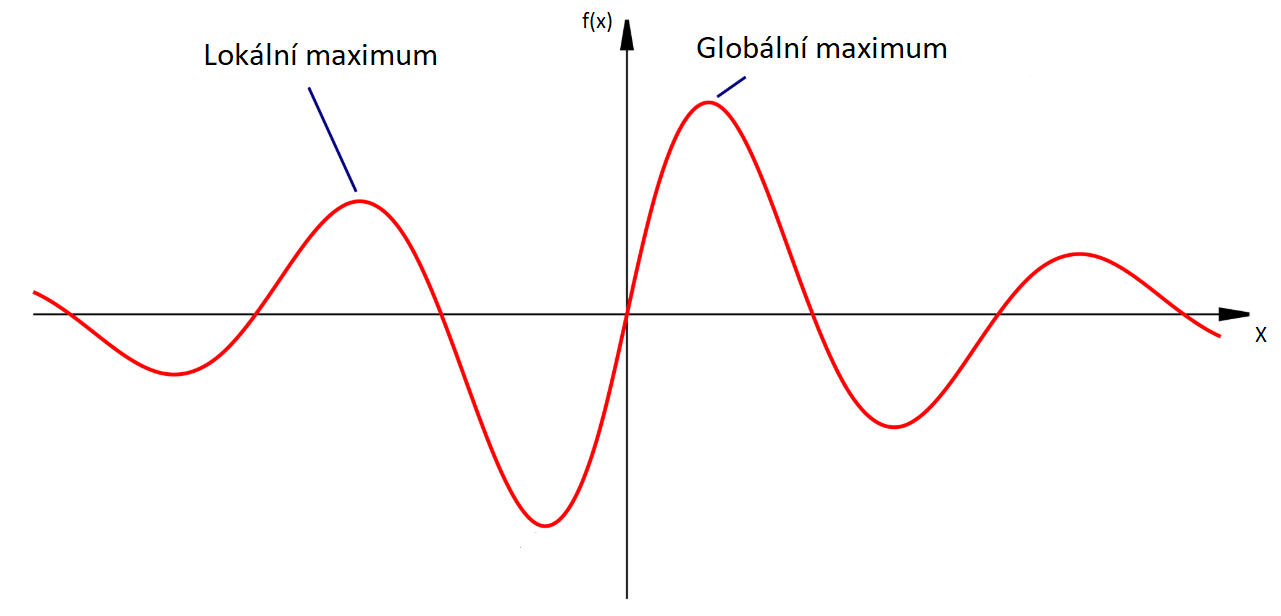
\includegraphics[width=\linewidth * 3/4]{obrazky-figures/localGlobal.png}
\caption{Ukázka globálního a lokálního minima na jednoduché matematické funkci. Zdrojem je internet.}
\label{fig:localGlobal}
\end{figure}


\subsection{Klasifikace optimalizačních úloh} \label{subsec:classific}
Dle definičního oboru prostoru \(\Omega\) účelové funkce se optimalizační úlohy klasifikují na:

\begin{itemize}
\item Úlohy volného extrému. Tento případ nastává, pokud \(\Omega = \mathbb{R}^n\).
\item Úlohy vázaného extrému - případ kdy \(\Omega \subset \mathbb{R}^n\). Zde nás zajímají pouze řešení, která splňují další podmínky, omezující buďto jeden nebo více vstupních parametrů \(x_0, ... x_n\) na interval, nebo funkcemi \(g_0(x_i, ... x_n) \geq 0 \). O~takto definovaných úlohách se mluví jako o~úlohách matematického programování. Jednoduché příklady omezení vázaného extrému jsou znázorněna na obrázcích~\ref{fig:BoxConstraint} a~\ref{fig:GeneralConstraint}.
\item Funkce jednoho extrému - tzv. \uv{unimodální}.
\item Funkce více extrémů stejné váhy - tzv. \uv{multimodální}.
\end{itemize}

\begin{figure}[!tbp]
\begin{minipage}[b]{0.450\linewidth}
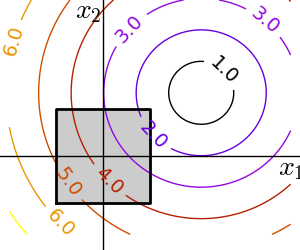
\includegraphics[width=\linewidth]{obrazky-figures/box_constraint.png}
\caption{Omezení intervalem.}
\label{fig:BoxConstraint}
\end{minipage}
\hfill
\begin{minipage}[b]{0.450\linewidth}
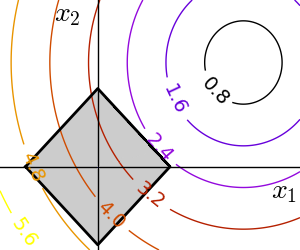
\includegraphics[width=\linewidth]{obrazky-figures/general_constraint.png}
\caption{Omezení funkcí.}
\label{fig:GeneralConstraint}
\end{minipage}
\end{figure}

\subsection{Operační výzkum} \label{subsec:OpRes}
Pojmem \emph{operační výzkum} (často označován také jako operační analýza) se všeobecně rozumí převod komplexní inženýrské úlohy reálného světa na matematický, či jiný, model a následné provádění experimentů pro získání informací. Problémy tohoto typu jsou často spojeny s~hledáním minima (např. provozní riziko), maxima (např. zisk), či jiného optimálního výsledku. Teoretickým základem operačního výzkumu je tedy matematická optimalizace a ke hledání řešení se využívá metody optimalizací, modelování a simulací~\cite{operResearch}.

Průběh operačního výzkumu je znázorněn na obrázku~\ref{fig:Operation_Research}. \\
\begin{figure}[h]
\centering
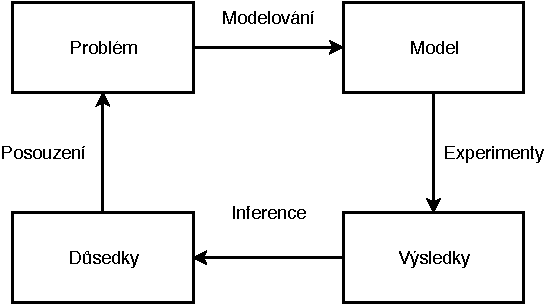
\includegraphics[width=\linewidth * 3/4]{obrazky-figures/operacniVyzkum.pdf}
\caption{Zjednodušený náhled na proces operačního výzkumu}
\label{fig:Operation_Research}
\end{figure}


\section{Fokusovaný ultrazvuk o~vysoké intenzitě}
\label{about:sec:hifu}
Fokusovaný ultrazvuk o~vysoké intenzitě je moderní technika pro ne-invazivní operace nádorových onemocnění, při které je maligní tkáň odstraněna kumulovanou tepelnou energií vyzářenou ultrazvukovými vysílači. Tato takzvaná termální ablace je provedena pod dohledem profesionála a úkolem je zvýšit teplotu v~cíleném místě o~několik desítek stupňů, čímž dojde ke zničení tkáně. Na rozdíl od standardních postupů léčby rakoviny se jedná o~ne-invazivní a ne-ionizující řešení, které již bylo aplikováno ve více než 100,000 případech.

Jedno toto ultrazvukové ozáření - tzv. sonikace - dokáže odstranit pouze malou oblast cílené tkáně. V~závislosti na velikosti oblasti ošetřované části může být potřeba absolvovat sérii těchto sonikací (běžně v~řádu desítek). Každá takováto sonikace může způsobit různá další zranění - od popálenin kůže až po možné vážné poškození tkáně poblíž fokálního místa a nebo někde mezi vysílačem a nádorem.

Hlavním problémem tohoto přístupu je tedy toto: jak rozmístit sérii ohnisek vysílačů v~prostoru tak, aby se minimalizovalo riziko zranění i počet sonikácí a zároveň byla zničena všechna nežádoucí tkáň. Navíc je třeba dát pozor na různé komplikace, jako například krevní řečiště sousedící s~cíleným tumorem, které může odvést velkou část indukované tepelné energie, nebo může být zářením poškozeno~\cite{BLOODOCCLUSION}. Série ohnisek sonikací poté vytváří trajektorii. Toto je optimalizační, přesněji minimalizační, problém, který svou povahou připomíná problém batohu - snažíme se co nejmenší vahou (zatížením těla sonikacemi) zaplnit co největší prostor (odstranit celou nežádoucí tkáň). Bohužel, běžné matematicko-fyzikální rovnice pro šíření zvukových vln a tepla spolu s~metodami optimalizace v~tak komplikovaném a heterogenním prostředí, jako může být i lidský mozek, a pro tak individuální systém selhávají, a je třeba přistoupit k~metodám operační analýzy a soft comuputingu - heuristiky a nebo algoritmy umělé inteligence. Tento přístup obětuje exaktní přesnost za rychlejší proces s~možností opakované, parametrizovatelné simulace spolu se zpětnou verifikací.



\begin{figure}[hbt]
	\centering
	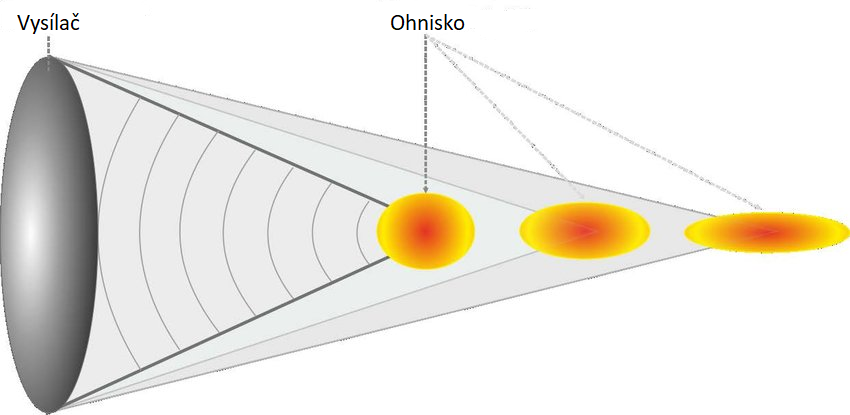
\includegraphics[width=0.7\textwidth]{obrazky-figures/ohnisko.png}
	\caption{Vizualizace regionů, ve kterém se indukuje teplo v~závislosti na vzdálenosti ohniska od vysílače. Převzato z~\cite{FITPUB11696}.}
	\label{focalRegion}
\end{figure}

\section{Rozšiřované řešení}
\label{about:sec:existSolution}
Jak již bylo nastíněno, k~řešení tohoto problému je třeba vytvořit model pro šíření tepla ve tkáních. Takovýto model byl již implementován v~nástroji k-Wave~\cite{HIFUTHERMALMODEL} a~využit v~řešení~\cite{FITPUB11696}.

\subsection*{Model} 
Průběh simulace modelu se skládá z~několika stádií. V~následujícím výpisu pouze nastíním jejich funkci, pro detailnější popis včetně referencí doporučuji již zmíněnou zdrojovou práci~\cite{FITPUB11696}:
\begin{itemize}
    \item \textit{Výpočet přidané tepelné energie ve tkáni} - v~závislosti na délce sonikace, pozici, velikosti a tvaru ohniska (znázorněno na obrázku~\ref{focalRegion}) je třeba zjistit, kolik tepelné energie bude vydáno zářením. Přesné výpočty jsou možné například za použití modelu ~\cite{HIFUPropagation}. Bohužel, tyto modely jsou příliš výpočetně náročné pro efektivní použití optimalizační metody, především pak pro použitou evoluční metodu. Proto bylo zavedeno několik zjednodušení a předpokladů. Tyto alternace jsou řádně ocitovány v~již zmíněném článku~\cite{FITPUB11696}.
    \item \textit{Šíření a rozptyl tepla ve tkáni} - dále je třeba zjistit, jak se všechno přidané teplo rozšířilo ve tkáních. Jedná se o~model Penneho biotepelné rovnice šíření, jejíž simulace je prováděna v~nástroji k-Wave~\cite{HIFUTHERMALMODEL}. Výstupem tohoto modelu je prostorová termální mapa (tzv. $CEM_{43}$ - Cumulative Equivalent Minutes at 43$^{\circ}$) kumulovaného tepla za sérii sonikací.
    \item \textit{Přesnost řešení}  - tato tepelná mapa je v~posledním kroku převedena na binární masku podle hranice. Následně je spočten integrál nad celou touto mapou, sčítající hodnoty oblastí, které byly ošetřeny a neměly být, spolu s~hodnotami oblastí, které neměly být ošetřeny a byly. Dále byla zavedena nevýznamná oblast - oblast ve které nás možná abraze nezajímá. Názorně zobrazeno na obrázku~\ref{fg:austinWoman}.
\end{itemize}

\subsection*{Plánování trajektorie}
K~návrhu a optimalizaci plánu byl použit algoritmus \uv{Covariance Matrix Adaptation - Evolutionary Strategy} - zkráceně CMA-ES. Jedná se o~moderní variantu evoluční strategie, pro nelineární nekonvexní systém černé skříňky definované na spojité veličině. Nevyžaduje náročné ladění parametrů - naopak výběr strategie vnitřních parametrů si algoritmus zvolí a postupně vylepšuje sám. Více se tímto algoritmem zabývá sekce~\ref{algs:cmaes}.

\subsection*{Kódování řešení}

Dále bylo také již navrženo kódování hledaných parametrů do chromozomu. Kandidátní řešení $I$ je poté trajektorie sonikací, kde $i$ odpovídá pořadí sonikací~\cite{FITPUB11696}: 
\begin{equation}
    \label{eq:trajectory}
     I~= (S_{1}, S_{2}, ..., S_{N})
\end{equation}kde
\begin{equation}
    \label{eq:S}
     S_{i} = (x(i), y(i), t_{on}(i), t_{off}(i)) 
\end{equation}
\begin{itemize}
    \item $S_i$ - parametry sonikace $i$
    \item $x(i), y(i)$ - 2D souřadnice ohniska sonikace $i$
    \item $t_{on}(i)$ - délka sonikace $i$
    \item $t_{off}(i)$ - interval ochlazení po dokončení sonikace $i$
\end{itemize}

\begin{figure}[hbt]
	\centering
	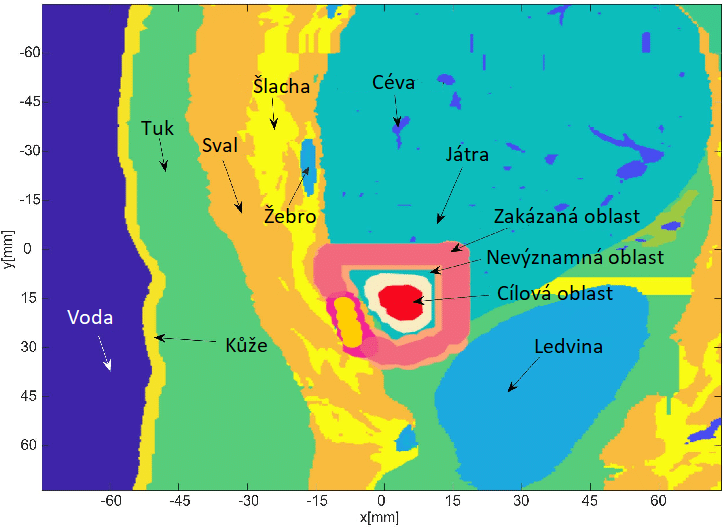
\includegraphics[width=0.7\textwidth]{obrazky-figures/austinWoman.png}
	\caption{Segmentová mapa AustinWoman s~vyznačenou cílovou, zakázanou a nevýznamnou oblastí. Převzato z~\cite{FITPUB11696}.}
	\label{fg:austinWoman}
\end{figure}


%https://www.kiv.zcu.cz/studies/predmety/uir/gen_alg2/E_alg.htm
%https://ieeexplore.ieee.org/stamp/stamp.jsp?tp=&arnumber=7955308
%https://www.vutbr.cz/www_base/zav_prace_soubor_verejne.php?file_id=31876
%https://wis.fit.vutbr.cz/FIT/st/cfs.php?file=%2Fcourse%2FEVO-IT%2Flectures%2F04-GenetickeAlg.pdf&cid=12093
\chapter{Evoluční algoritmy} 
\label{algs}
\textit{Evoluční algoritmy} (zkráceně EA) patří do kategorie přírodou inspirovaných algoritmů. Jedna se o~zastřešující množinu pro různé přístupy, které se inspirují v~evolučním procesu - pokud je populace jedinců vystavena dlouhodobě selekčnímu tlaku, začíná se v~následujících generací na tento tlak lépe adaptovat, aby druh přežil. Takto adaptovaní jedinci dále šíří své geny a neustále vylepšují zdatnost následujících populací. Z~technického pohledu je množina jedinců (generace) iterativně vystavována evolučním operacím (v~genetickém algoritmu jsou to operace selekce nejlepších jedinců, jejich křížení a případně mutace potomků) pro vytvoření generace nové. Zda-li se původní jedinci budou či nebudou nacházet v~nové populaci již záleží na implementaci samotné. 

Z~matematického hlediska se řadí mezi stochastické metody prohledávání stavového prostoru a \textit{metaheuristiky} - strategie, či procedura na nějaké vyšší úrovni, jejíž cílem je nalézt proceduru nebo heuristiku o~úroveň níže, která bude schopná řešit zadaný problém bez bližších údajů o~optimalizovaném systému~\cite{EA_OVERVIEW}.

Již mnohokrát se ukázalo, že EA dokáží najít inovativní či zcela nová řešení inženýrských úloh, která konvenční algoritmy nejsou schopna poskytnout~\cite{EVO}. \\

\noindent Oproti konvenčním optimalizačním metodám vykazují EA především tyto vlastnosti:
\begin{itemize}
    \item Výhody \begin{itemize}
         \item Jednodušší a flexibilnější návrh - není třeba pokročilých znalostí matematiky či fyzikálních principů k~použití těchto algoritmů.
         \item Umožňují optimalizovat systémy o~kterých nemají žádné informace. 
        \item Pokud ovšem tyto informace máme, jsme schopni je využít ke zrychlení/zefektivnění optimalizace.
        \item Robustnost a schopnost přizpůsobit se změnám v~prostředí či prostředí samotného a šumu.
        \end{itemize}
    \item Nevýhody \begin{itemize}
        \item Samotná povaha metod je stochastická a tedy nezaručuje optimálnost řešení.
        \item Algoritmy této rodiny jsou často velice náchylné na nastavené parametry a špatné zvolení těchto parametrů vede na selhání.
        \end{itemize}
\end{itemize}

Další rodina algoritmů, která se do skupiny evolučních algoritmů zařadila nedávno, se nazývá \textit{Memetické algoritmy}, nebo také kulturní algoritmy či genetické lokální prohledávání~\cite{EA_OVERVIEW}. Na rozdíl od evoluce celých populací se zaměřují na evoluci jedinců - selekčním tlakem zde není schopnost přežití v~přírodě nýbrž ve společnosti.

\begin{figure}[hbt]
	\centering
	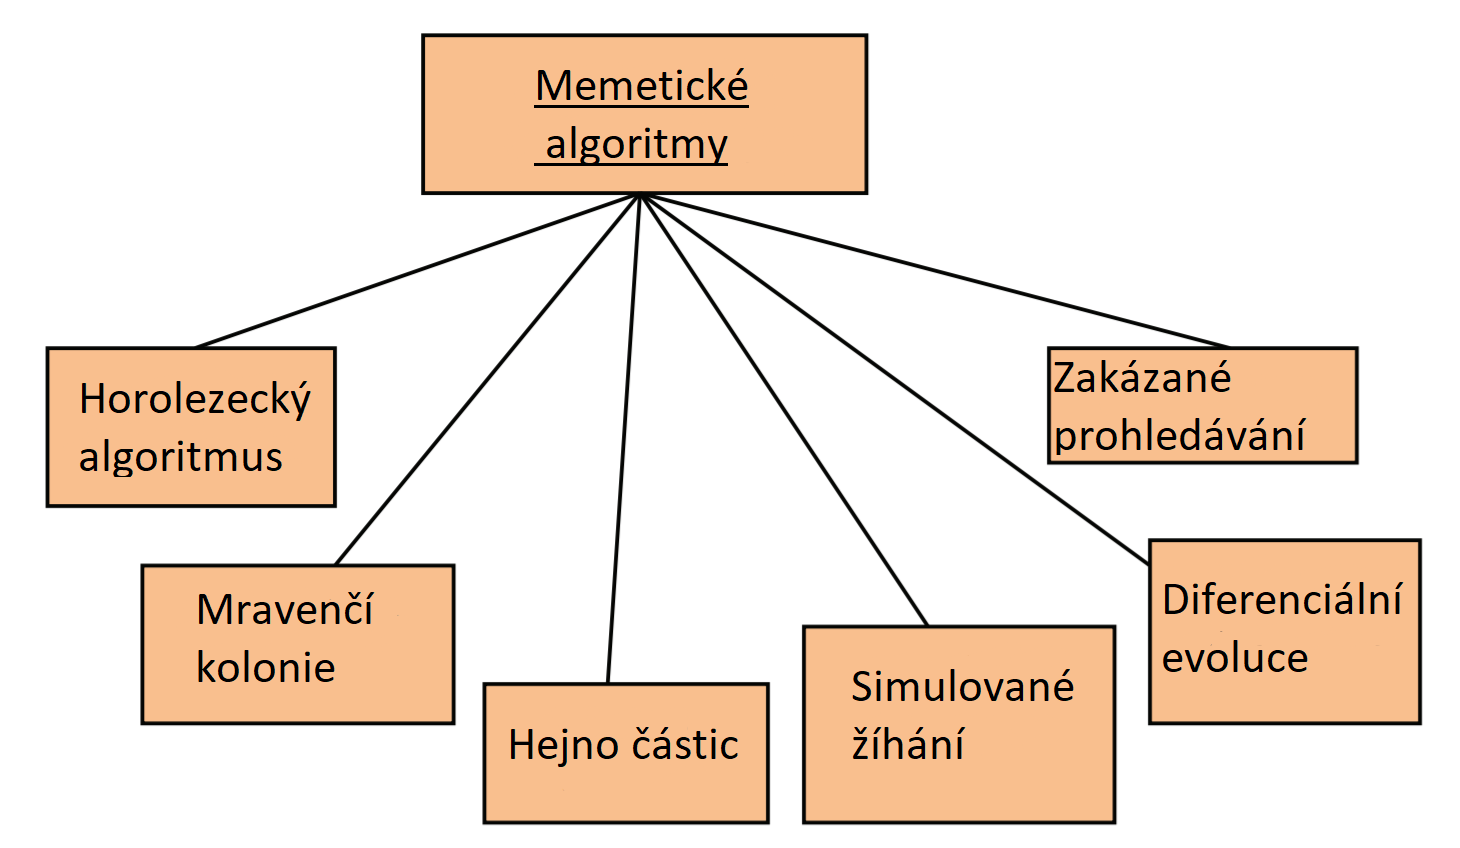
\includegraphics[width=0.85\textwidth]{obrazky-figures/memetic.png}
	\caption{Memetické algoritmy. Převzato z~\cite{EA_OVERVIEW}}
	\label{fg:memtic}
\end{figure}

\subsection*{Selekční tlak}
Při prohledávání stavového prostoru je neustále třeba hledat rovnováhu mezi prohledáváním a \uv{vykořisťováním}~\cite{EVO}. Prohledávání nutí jedince v~populaci pokrýt celou plochu prohledávaného prostoru a vykořisťování umožní jedincům specializovat se v~nějaké podoblasti prostoru a skutečně konvergovat k~optimálnímu řešení v~tomto podprostoru~\cite{Weisser2010}. Tato síla se nazývá selekční tlak a pohání každý EA. Velikost selekčního tlaku ovlivňuje tendence algoritmu prohledávat a vykořisťovat. Čím větší je selekční tlak, tím menší stavový prostor algoritmus prohledává a tím více je hnán ke konvergenci k~optimu v~tomto podprostoru a naopak~\cite{Weisser2010}.

\subsection*{Pojmy}
Následuje výčet a vysvětlení používaných pojmů v~evolučních algoritmech~\cite{EVO}. Tyto pojmy mají svůj základ v~biologii, přesněji v~DNA a RNA~\cite{EA_OVERVIEW}:
\begin{itemize}
    \item \textit{Fenotyp/jedinec} - objekt a potencionální řešení daného problému.
    \item \textit{Chromozom/genotyp} - struktura řešení pro algoritmus. Konkrétní podoba chromozomu představuje jeden stav prohledávaného prostoru. Jeho interpretací získáváme fenotyp.
    \item \textit{Gen} - element chromozomu .
    \item \textit{Alela} - hodnota genu.
    \item \textit{Lokus} - pozice genu v~chromozomu.
    \item \textit{Populace} - struktura $n$ chromozomů. Multimnožina.
    \item \textit{Generace} - jedna iterace. Každá generace má svou populaci, na kterou jsou v~průběhu generace aplikovány genetické operátory. Výsledkem těchto operací je nová populace.
    \item \textit{Genetické operátory} - způsob a postup tvorby potomků z~rodičovských chromozomů.
    \item \textit{Ukončovací podmínky} - podmínka, při které je evoluce prohlášena za dokončenou. Typicky dosažení požadovaného výsledku nebo dosažení maximálního počtu generací.
    \item \textit{Fitness funkce} - funkce vyhodnocující  stupeň adaptace jedince s~ohledem na kritéria a cíle evolučního procesu, zjednodušeně schopnost jedince přežít.
    \item \textit{Prohledávaný prostor} - množina všech potencionálních řešení problému. Každý bod v~tomto prostoru má jistý potenciál pro přežití; svou fitness. Velikost a tvar tohoto prostoru je závislý na množině potencionálních řešení optimalizovaného problému. Zároveň ze znalosti řešeného problému mohou vyplynout další podmínky, které tento prostor dále omezí - tzv. omezující podmínky. Tato omezení nemusí a často nebývají lineární - například omezení křivkou nelineární funkce derivace některé z~proměnných.
\end{itemize}

Příklad: Pokud je fenotypem ASCII znak, chromozomem bude struktura osmi bitů, genem bit, alela bude hodnota 1 či 0 a lokus bude pozice zvoleného genu v~rámci znaku (0 - 7).

\section{Genetický algoritmus}
\label{algs:ga}
Genetický algoritmus (GA) je jedním z~nejpopulárnějších z~rodiny EA. Byl inspirované Darwinovou teorii evoluce a jako první jej popsal John Holland v~roce 1975~\cite{GAIntro}. Často je používán při strojovém učení, rozpoznávání a klasifikace a pro optimalizace. GA je populačně zaměřený EA a jako evoluční operace používá křížení a mutaci. Genetický algoritmus je běžný ve dvou variantách:
\begin{itemize}
    \item \textit{Generační model}, v~literatuře často \uv{generation GA} - vždy je celá populace jedinců nahrazena následující populací.
    \item \textit{Ustálený model}, v~literatuře \uv{steady-state GA} - v~každé generaci je nahrazován jen nejhorší jedinec.
\end{itemize}

\bigskip

Algoritmus začíná s~nějakou, typicky náhodně vygenerovanou, populací chromozomů. Každý jedinec populace je jedním řešením daného problému a principem je postupně se v~průběhu generací za pomoci genetických operátorů dostávat k~novým a kvalitnějším jedincům. Ohodnocení kvality každého z~jedinců probíhá za pomoci fitness funkce, která je specifická pro řešený problém. Toto je prováděno do té doby, dokud není splněno nějaké ukončovací kritérium. Flowchart~\ref{fg:gaFlow} ukazuje rozhodovací proces algoritmu.\\

\begin{figure}[hbt]
	\centering
	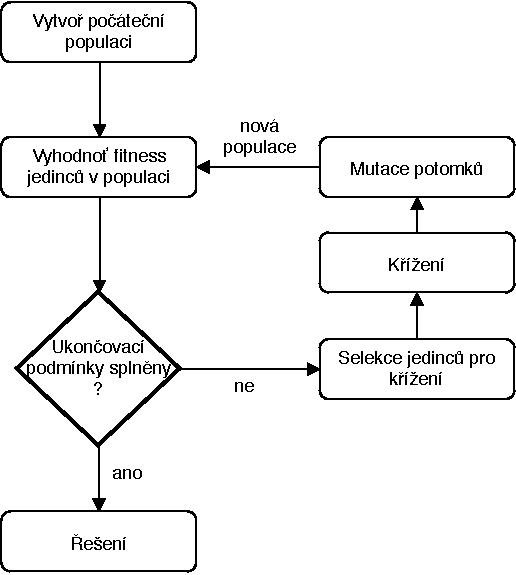
\includegraphics[width=0.6\textwidth]{obrazky-figures/gaFlow.pdf}
	\caption{Flowchart průběhu genetického algoritmu.}
	\label{fg:gaFlow}
\end{figure}

\subsection{Kódování chromozomu}
Jedná se o~způsob, jakým je reprezentována struktura chromozomu. Lze uvažovat například kódování binární - 8 bitů tvoří chromozom a každý bit je jedním genem. Nebo také ale bity nemusí být pro nás významnou hodnotou a chromozomem je například binární strom, či seznam prvků nebo i~obyčejné číslo (reálné nebo i přirozené). 

\subsubsection*{Binární kódování}
Původní varianta GA používala právě toto kódování. Typickým případem použití tohoto kódování jsou problémy, jejichž jedinci nejsou definováni na množině čísel, případně potřebujeme velkou kontrolu nad evolucí jedinců. Nevýhodou použití tohoto kódování pro číselné~typy, respektive typy, na nichž je definována relace uspořádání je tzv. \textit{Hammingova bariéra} - malá změna v~genotypu jedince může způsobit velké změny fenotypu. Například čísla $127d = 01111111b$ a $128d = 10000000b$. Toto může snižovat výkonnost algoritmu~\cite{Weisser2010}. Jedním z~možných řešení je tzv. \textit{Grayův kód} - binární kódování čísel, ve kterém se sousední hodnoty vždy liší pouze v~jednom bitu. Pro ukládání reálných čísel je nejdříve třeba tyto čísla převést na celá čísla. 

\subsubsection*{Číselné}
Typicky používáno pro optimalizační úlohy definované na množině $\mathbb{N}$ či $\mathbb{R}$. V~takovýchto úlohách se běžně pracuje s~číselnými fenotypy a není třeba nižší úrovně ukládání hodnot. Dalším příkladem použití celočíselných chromozomů je \textit{pořadové kódování}, které se používá pro úlohy hledání cest. Poté může být každý uzel reprezentován jedním číslem a~chromozom obsahovat seznam čísel, jejichž pořadí udává pořadí, ve kterém jsou uzly navštíveny.


\subsection{Selekce}
Představuje postup, jakým jsou vybírány chromozomy aktuální populace pro proces křížení~\cite{EVO, Weisser2010}. Následně jsou uvedeny nejběžněji používané selekční operátory.

\subsubsection*{Turnaj}
Náhodně vybráno $m$ jedinců, kteří se účastní turnaje. Vítěz tohoto turnaje je poté vybrán pro křížení. Podmínky pro vítězství v~turnaji se mohou lišit, typické je ovšem použít hodnotu fitness. 

\subsubsection*{Vážená ruleta}
Pravděpodobnost výběru každého jedince závisí na jeho fitness hodnotě a na fitness hodnotě zbytku populace. Představme si ruletu, kterou roztáčíme pokaždé, když chceme vybrat jedince. Čím lepší fitness má jedinec vzhledem ke zbytku populace, tím větší je jeho část rulety a tedy tím větší šanci má, že bude vybrán~\cite{EVO, Weisser2010}.

\subsubsection*{Rank}
Jedinci v~populaci jsou seřazení podle své fitness od nejlepšího k~nejhoršímu. Každému jedinci je přiřazeno číslo $k$, které například určuje, kolik jedinců v~populaci je horších, než je on sám. Následně je dle tohoto čísla spočítána pravděpodobnost každého jedince k~výběru~\cite{EVO, Weisser2010}.

\subsubsection*{Elitismus}
Nejlepšího jedinec (případně $n$ nejlepších) přežije svou generaci a dostane šanci uplatnit se v~následující. Takovýto jedince přeskakuje evoluční operátory. Elitismus má potenciál snižovat diverzitu populace a naklánět selekční tlak spíše k~vykořisťování~\cite{EVO}. Jedná se o~emergentní~\ref{def:emergence} vlastnost některých selekčních operátorů. V~případech, kdy nepoužíváme tyto operátory, můžeme tuto vlastnost algoritmu zavést explicitně. 

\subsubsection*{Incest}
Jedince s~podobnými chromozomy lze považovat za příbuzné a pokud by mělo dojít ke křížení takovýchto jedinců, nevznikne žádná nová vlastnost. Tento jev snižuje diverzitu populace a může vést k~předčasné konvergenci a je třeba se mu bránit. Tuto situaci lze detekovat za pomoci \textit{Hammingovy vzdálenosti}, případně \textit{Euklidovské metriky}. Pokud jsou dva jedinci vybraní k~páření příbuzní, je třeba zamezit křížení a provést selekci nového jedince~\cite{Weisser2010}.

\subsection{Křížení}
Je kombinací rodičovských genů za cílem vytvoření potomstva. Má význam pro zvýšení schopnosti explorace algoritmu a zajištění diverzity, ovšem také ke schopnosti algoritmu konvergovat. Spolu s~vhodnou selekční metodikou tlačí populaci k~jedincům s~lepšími vlastnostmi. V~základním provedení 2 rodiče produkují 2 potomky. Následující varianty operace křížení předpokládají standardní binární či celočíselnou reprezentaci. Pokročilejší zakódování vyžadují speciální návrhy těchto operátorů. V~případě číselných chromozomů je možné pro křížení použít například operace průměru či sečtení~\cite{EVO, Weisser2010}. 

\begin{figure}[!tbp]
\begin{minipage}[b]{0.485\linewidth}
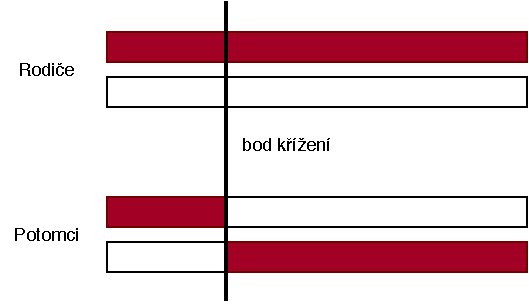
\includegraphics[width=\linewidth]{obrazky-figures/cross_onepoint.pdf}
\caption{Jednobodové křížení.}
\label{fig:EA_1Cross}
\end{minipage}
\hfill
\begin{minipage}[b]{0.485\linewidth}
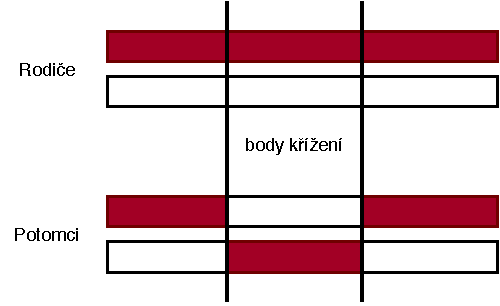
\includegraphics[width=\linewidth]{obrazky-figures/cross_multipoint.pdf}
\caption{Vícebodové křížení.}
\label{fig:EA_2Cross}
\end{minipage}
\end{figure}

\subsubsection*{Jednobodové}
V~chromozomech o~délce $n$ je náhodně zvolen index $i, 1 \leq i \leq n$. Prvních $i$ genů je poté získáno z~prvního rodiče, zatímco $i$ až $n$ z~druhého rodiče. Záměnou pořadí rodičů můžeme získat až dva potomky~\cite{Chlebik2017}. Znázorněno na obrázku~\ref{fig:EA_1Cross}.

\subsubsection*{Vícebodové}
Analogicky k~jednobodovému křížení, je vygenerováno až $k$ různých indexů $(i_0, ... i_k)$, pro které platí $(1 \leq i_1 \le i_2 \le ... \le i_k \le n)$. Poté se vybere náhodný rodič, ze kterého je zkopírována část $i_j$ až $i_{j+1}$, posune se index $j$ a rodiče alternují. Záměnou pořadí je i zde možné získat dva potomky~\cite{Chlebik2017}. Znázorněno na obrázku~\ref{fig:EA_2Cross}.
 
\subsubsection*{Uniformní}
Každému genu je vygenerována rovnoměrným rozložením zvoleno, ze kterého z~rodičů bude gen zkopírován. Záměna rodičů opět umožní získání druhého potomka.


\subsection{Mutace}
Klíčový genetický operátor z~pohledu přínosu nových vlastností jedinců~\cite{EVO, Weisser2010}. Obvyklým postupem je zcela náhodná změna několika náhodně vybraných genů u~náhodně vybraných jedinců. Smyslem mutace je zvyšovat diverzitu populace. Pravděpodobnost výskytu mutace se typicky volí jako nízká; při neúměrně vysoké mutaci totiž může docházet k~narušování dříve slibných řešení před konvergencí k~optimu. Ovšem příliš nízká mutace může vést na nedostatečnou diverzitu populace a s~tím spojené omezené schopnosti GA prohledávat stavový prostor.
V~binárních chromozomech můžeme náhodně měnit bity, v~číselných například náhodně přičíst konstantu nebo vynásobit chromozom nějakou váhou či maskou~\cite{Chlebik2017}.

\section{Simulované žíhání}
\label{alg:sa}
Metoda simulovaného žíhání patří mezi memetické algoritmy a její základ je v~metalurgii, přesněji ve fyzikálním jevu žíhání - procesu, při kterém je těleso umístěno do pece vyhřáté na vysokou teplotu a~postupným pomalým ochlazováním jsou odstraňovány vnitřní defekty tělesa. Po dokončení je ocel stejně pevná ovšem ohebnější a~odolnější vůči poškození.

Při vysokých teplotách je těleso v~tekutém stavu, krystalová mřížka náhodně uspořádána s~krystalky kmitajícími v~prostoru - systém je ve stavu vysoké entropie. Postupným ochlazováním se celková entropie systému snižuje - krystalky mřížky přestávají kmitat a~pomalu se usazují do pozic s~nižší energií. Celý systém se tak dostává do rovnovážného stavu s~pevnou mřížkou bez defektů.

Algoritmus simulovaného žíhání následuje tento princip. Tělesem je náš optimalizovaný systém, u~kterého se předpokládá, že začíná ve stavu vysoké entropie. Kandidátní řešení algoritmu je potom energie systému, přesněji uspořádání krystalků mřížky. 
Postupem času se systém ochlazuje dle nějakého předem zvoleného chladícího rozvrhu a~mřížka se ustaluje - v~každém kroku jsou zaváděny náhodné poruchy momentálního stavu (je prohledáváno blízké \uv{okolí} současného stavu) a~je porovnávána energie při těchto defektech s~energií momentální. V~případě, že některá z~poruch má nižší energii, než stav momentální, určí jej algoritmus za nejlepší řešení v~rámci této iterace a~přijme jej za nový výchozí stav. V~případě, že se nenašel lepšího kandidáta, je proveden test na \textit{Metropolisovo kritérium}. Pokud je test úspěšný je i~horší stav přijat za momentální. Toto kritérium je založeno na Boltzmannové pravděpodobnostním rozdělení a~šance na přijetí klesá spolu s~teplotou~\cite{fitWebSA}: 

\begin{equ}[!ht]
\begin{equation}
\label{eq:boltz1}
W_T(E_i) = \frac{1}{Z(T)}\exp(\frac{-E_i}{k_BT})
\end{equation}
\end{equ}
kde  $T$ je teplota žíhaného tělesa, $E_i$ je energie systému ve stavu $i$, $k_B$ je Boltzmannova konstanta. Partiční funkce Boltzmannova rozdělení $Z(T)$ je rovnice \ref{eq:boltz2}:
\begin{equ}[!ht]
\begin{equation}
\label{eq:boltz2}
Z(T) = \sum_{j}\exp(\frac{-E_j}{k_BT})
\end{equation}
\end{equ}
\\
Znázorněno na obrázku \ref{fg:cooling}.

\subsection{Boltzmannovo rozdělení}
Za podmínky, že proces ochlazování je dostatečně pomalý je žíhaný systém vždy rovnovážném stavu - tento jev popisuje \textit{Boltzmannovo rozdělení pravděpodobnosti} (rovnice \ref{eq:boltz1} a~\ref{eq:boltz2}). V~případě, kdy dochází k~ochlazování systému příliš rychle mohou defekty zamrznout a vzniknout tak metastabilní struktury - lokální minima - které SA nedokáže překonat ~\cite{fitWebSA}. Pro simulaci tohoto rozdělení lze použít, a~v~metodě simulovaného žíhání se používá, algoritmus \textit{Metropolis}, který je implementací metody \textit{MCMC - Markov Chain Monte-Carlo}~\cite{webMCMC}.


\subsection{Monte Carlo a Markovské řetězce}
Monte Carlo je stochastická numerická metoda pro získávání znalostí o~simulovaných systémech pracující s~teorií pravděpodobnosti. Metoda provádí $n$ náhodných pokusů se systémem a po dokončení statisticky odhaduje charakteristiku systému. Metoda \textbf{Monte Carlo} je modelování takové náhodné veličiny $X$, že její střední hodnota $E(X)$ je rovna hledané hodnotě $a$. Pak, jestliže vypočteme $n$ nezávislých realizací $X_1, ..., X_n$ náhodné veličiny $X$, můžeme odhadnout $a$ pomocí aritmetického průměru~\cite{MonteCarlo}.
\\\\
 Předpokládejme, že máme diskrétní množinu hodnot a jí odpovídající diskrétní množinu výsledků - stavů. Poté můžeme \textbf{Markovův řetězec} použít pro popis modelu tohoto systému~\cite{NahodneProcesy, EVO}. Zjednodušeně - jedná se o~model série událostí, které jsou v~nějakém pravděpodobnostním vztahu. Na základě statistiky tento model předpovídá, jaká událost nastane příště bez znalosti předchozích událostí - model nemá paměť. (tzv. \textit{Markovská vlastnost}).
 \\\\
 Spojením těchto dvou modelů získáváme \textbf{Markov Chain Monte-Carlo (MCMC)}. Metodu, která stejně jako Monte Carlo získává znalosti o~systému za pomoci náhodných pokusů, ovšem tyto náhodné pokusy vytváří stavy markovského řetězce, který vykazuje vlastnost zvanou \textit{ergodicita}~\cite{EVO}. Ergodicitní modely, mimo jiné, naleznou rovnováhu v~náhodném rozložení a ustálí se kolem tohoto stavu (tzv. stacionární rozdělení). Markovské řetězce také zavádějí závislosti mezi momentálním a následujícím stavem ve zkoumané distribuční funkci. Analýzou takto vzniklého řetězce jsme schopni získat informace o~systému, které obyčejné Monte Carlo nedokáže. MCMC je také mnohem vhodnější pro získávání vzorků z~více-dimenzionálních distribučních funkcí. Problémem tohoto přístupu je hlavně citlivost na zvolený počáteční stav. Dále pro ně platí \uv{halting problem} - nevíme, jestli řetěz již konvergoval~\cite{webMCMC}.

\begin{figure}[hbt]
	\centering
	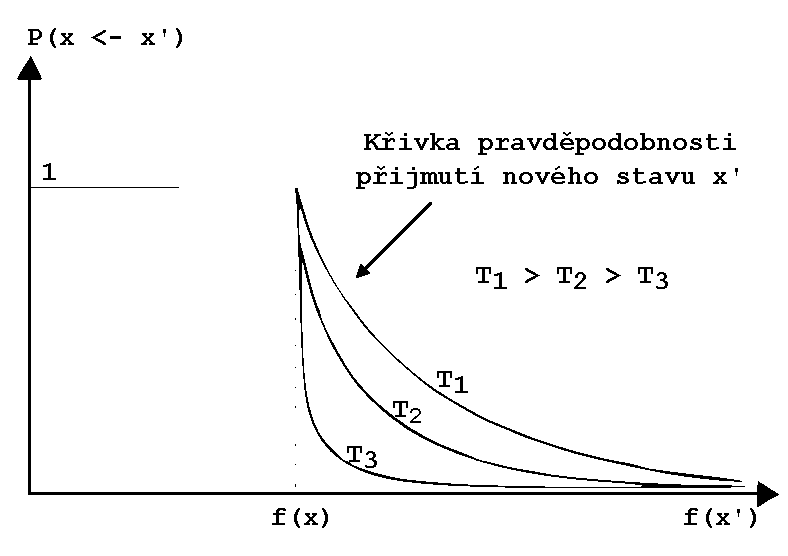
\includegraphics[width=0.5\textwidth]{obrazky-figures/cooling.pdf}
	\caption{Křivka pravděpodobnosti přijetí horšího řešení v~závislosti na teplotě systému. Zdroj: internet.}
	\label{fg:cooling}
\end{figure}

\subsection{Metropolis}
Algoritmus Metropolis~\cite{webMCMC} je MCMC metoda pro získávání náhodných vzorků z~pravděpodobnostní distribuce, u~které je toto vzorkování složité a nebo je distribuční funkce více-dimenzionální. Algoritmus vznikl jako způsob, jak počítačovou simulací zajistit vlastnosti termodynamického systému za pomoci MCMC metody. Pseudokód algoritmu je možné vidět na \ref{code:metropolis}. Algoritmus cyklicky provádí následující:
\begin{itemize}
    \item Vygeneruj kandidátní řešení za pomoci funkce zvané \uv{kernel}. Tato funkce je poskytnuta uživatelem a může být třeba i funkcí generující náhodné čísla. V~případě SA je to funkce \textbf{perturberance} - \ref{eq:perturb} - která je volená tak, aby byla symetrická; pravděpodobnost toho, že malou poruchou se ze stavu A~stane stav B je stejná, jako že ze stavu B se stane stav A. Symetričnost kernel funkce je podmínkou algoritmu Metropolis (ovšem SA funguje i bez splnění tohoto kritéria) 
    
    \item Vygeneruj akceptační kritérium - funkce pravděpodobnosti, která určuje, jak moc se navržené řešení liší od skutečného stavu navrženého Markovským řetězem (stacionární distribuce zmíněná dříve). v~případě SA se jedná o~\textbf{Metropolisovo kritérium}~\ref{eq:metropolisCriter}~\cite{fitWebSA}~\cite{webMCMC}.
    \item Pokud jsou si dostatečně podobné, vygenerovaný stav je přidán do Markovského řetězu~\cite{webMCMC}.
\end{itemize}

\begin{equ}[!ht]
\begin{equation}
\label{eq:perturb}
x_{i+1} = x_i + u~* |x^{max} - x^{min}| * \frac{T}{T^{max}}
\end{equation}
\caption{Funkce perturberance - výběru kandidátního stavu. }
\end{equ}
kde $u$ je náhodné číslo rovnoměrného rozložení mezi $-1$ a $1$, $x_i$ je fitness momentálního stavu, $x^{max}$ a $x^{min}$ jsou fitness hodnoty prozatím nejhoršího a nejlepšího nalezeného stavu resp., $T$ je momentální teplota systému a $T^{max}$ je počáteční teplota.

\begin{equ}[H]
\begin{equation}
\label{eq:metropolisCriter}
\exp(-(\frac{\Delta E}{T_i}))
\end{equation}
\caption{Metropolisovo kritérium pro přijetí horšího stavu v~simulovaném žíhání.}
\end{equ}

\subsection{Rozvrh chlazení}
Většina parametrů simulovaného žíhání - definiční obor, výběr následujícího stavu, atd. - jsou dány již v~definici a za běhu se nemění. O~to více důležitý je pro nalezení optima výběr správného chladícího rozvrhu. Běžně je nejpoužívanější lineární rozvrh chlazení. Ten lze vyjádřit následovně~\cite{Chlebik2017}:

\begin{equ}[H]
\begin{equation}
\label{eq:cooling}
T(i) = T_0 * \alpha^i
\end{equation}
\caption{Běžný lineární rozvrh chlazení systému SA. $(0 \le \alpha \le 1) $}
\end{equ}

Pro vhodně malé $\alpha$, je tento rozvrh dostatečně pomalý a umožní globální konvergenci.

\subsection{Algoritmus}
Pseudokód algoritmu simulovaného žíhaní \cite{Chlebik2017} využívající metodu Metropolis je definován v~algoritmech~\ref{code:SA} a~\ref{code:metropolis}. Je vhodné podotknout, že parametry funkcí například $Perturb$ se považují za proměnné v~globálním prostoru.

\floatname{algorithm}{Algoritmus}
\vspace{\baselineskip}
\begin{algorithm}[H]
\begin{algorithmic}
\State $T := T_{max};$ 
\State $x_{best} := $ náhodně vygenerovaný stav;
 \While{$T > T_{min}$}
 	\State $x_{best} := Metropolis();$
 	\State $T := T * \alpha;$
\EndWhile
\State \Return $x_{best};$
\end{algorithmic}
\caption{Algoritmus simulovaného žíhání}
\label{code:SA}
\end{algorithm}
\begin{algorithm}[H]
\caption{Metropolis}
\label{code:metropolis}
\begin{algorithmic}
  \State $k := 0;$ 
  \State $x_{new} := x_{best};$
 \While{$k < k_{max}$}
 \State $k := k + 1;$
 \State $x_{new} := Perturb();$
 \State $P := \min (1, \frac{exp(-(f(x_{new}) - f(x_{best}))}{T}));$
\If {$random() \leq P$} 
        \State $x := x_{new};$
\EndIf
\EndWhile
\State \Return $x_{new};$
\end{algorithmic}
\end{algorithm}



\section{Tabu prohledávání} %tabu search
\label{algs:ta}
Zakázané prohledávání - častěji v~originálním názvu \uv{Tabu prohledávání} či \uv{Tabu strategie} - je globální optimalizační metoda a meta-heuristika zastřešující rodinu metod, které vnášejí do optimalizačních algoritmů paměťové struktury pro překonání lokálního optima~\cite{Glover2006}. Tabu prohledávání je založeno na premise, že každé řešení problému, které lze klasifikovat jako inteligentní, musí začlenit do svého systému adaptivní paměť, a neslepé, reagující prohledávání. Poté, pokud systém s~pamětí udělá špatnou volbu, je možné se z~této volby díky paměti poučit a upravit strategii. To je v~kontrastu s~návrhem dalších optimalizačních metod založených na přírodních jevech, jakou je například \textit{Simulované žíhání}~\cite{Glover2006}. Tabu prohledávání dostalo své jméno od slova Tabu - \textit{zakázaný} - kvůli své inspiraci v~kulturní evoluci (tabu prohledávání je memotický a evoluční algoritmus). V~kontextu společnosti jsou \uv{tabu} věci taková témata, o~která společnost nestojí a jedinec, který na toto nedbá, bude na nižším společenském postavení a tedy nemusí přežít. 

\subsection{Horolezecká metoda}
\textit{Horolozecký algoritmus}, iterativně prochází stavový prostor. Vždy se z~momentálního stavu rozhlíží po okolí a~pokud je některý z~těchto okolních stavů lepší, přijme jej za současný. Tato logika je opakována po $k$~iterací nebo dokud není dosaženo některé z~ukončovacích podmínek. Takto nejlepší nalezený jedinec je prohlášen za optimum a~algoritmus ukončen. Tato metodika často vede na uváznutí v~oblastech lokálního optima - stav, kdy všechny relativně blízké stavy mají horší fitness. Tento problém je elegantně řešený Tabu strategií zavedením paměti - tzv. Tabu seznamu. Tabu úpravu běžného horolezeckého algoritmu je možné vidět na obrázku~\ref{fg:tabu}.

\begin{figure}[hbt]
	\centering
	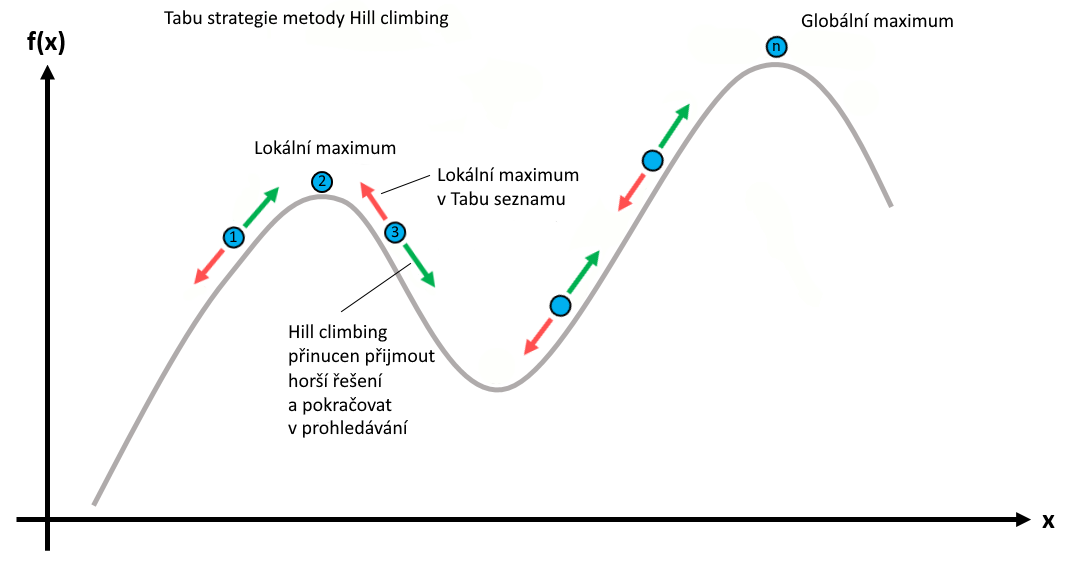
\includegraphics[width=0.8\textwidth]{obrazky-figures/tabu.png}
	\caption{Příklad využití strategie Tabu prohledávání nad lokální heuristikou Horolezecké metody (Hill climbing). Bez použití tabu strategie by se Hill climbing dopracoval do stavu $3$, ve kterém by lokálním prohledáním znovuobjevil stav $2$ a přesunul by se do něj.}
	\label{fg:tabu}
\end{figure}

\subsection{Adaptivní paměť}
Na rozdíl od běžných lokálních metod tedy Tabu strategie pracuje se skutečně dynamickým sousedstvím. Tabu prohledávání posouvá lokální heuristiky tak, že upravuje okolí $N(x)$ ($x$ je momentální stav), ze kterého mohou vybírat následující řešení. Toto nové okolí - $N*(x)$ - je omezováno třemi různými typy pamětí~\cite{gloverArt}: 
\begin{itemize}
    \item \textit{krátkodobá paměť} - jednoduchý seznam obsahující $n$ posledně navštívených stavů, kde $n$ je vstupním parametrem algoritmu. Všechny stavy v~tomto seznamu jsou vyloučeny ze sousedství.
    \item \textit{střednědobá paměť} - pravidla, jejichž účelem je vést vyhledávání ke slibným oblastem stavového prostoru. Zde se reálně budou nacházet omezující podmínky specifické pro řešený problém, případně pravidla urychlující konvergenci zakázáním jistých vzorů při vyhledávání.
    \item \textit{dlouhodobá paměť} - pravidla pro udržení diverzity.
\end{itemize}
Rozdíly, mezi těmito druhy pamětí jsou často velice mlhavé a co je pro jeden problém údaj střednědobý, může být v~jiné údajem dlouhodobým nebo naopak. Toto je navíc pouze zjednodušený náhled; koncept těchto pamětí je mnohem složitější a její rozbor pro tuto práci není podstatný. Je pouze vhodné dodat, že adaptivní paměť tabu strategie se dále dělí na nedávnou a opakující  -
\textit{nedávná} ukládá samotné vlastnosti řešení, které se změnily v~nedávné době (jedná se o~jistou úroveň granulity - nezakazujeme celé stavy ale například stavy, jejichž jedna vlastnost je omezena). \textit{Opakující} poté, jak název napovídá, zamezuje cesty, které vedou na cyklus či předčasné konvergenci jedné vlastnosti .
Pro zájemce doporučují například tento článek~\cite{gloverArt} samotného autora algoritmu, ve kterém se této problematice věnuje do hloubky.

\subsection{Algoritmus}
Pseudokód zakázaného prohledávání využívající Horolezeckou metodu je definován v~algoritmu~\ref{code:tabu}. Je vhodné podotknout, že se jedná o~vysokou abstrakci, která prezentuje pouze hlavní smyčku optimalizace a vynechává implementace metod pracujících s~tabu seznamem. $N(x)$ je sousední funkce tak, jak je definována optimalizovaným problémem, $StopCondition()$ je metoda ukončující optimalizace - například dosažením maximálního počtu iterací nebo nalezením optima, pokud je známé.
\begin{algorithm}[H]
\begin{algorithmic}
\State $TabuList := InicializujTabuList();$ 
\State $x_{best}$ := náhodně vygenerovaný stav;
 \While{$! UkoncovaciPodminka()$}
    \State $N^*(x) := Sousedstvi(N(x), TabuList)$
 	\State $x := HillClimbingKrok(x, N^*(x));$
 	\If{$Fitness(x) \leq Fitness(x_{best})$}
 	\State $x_{best} := x$
 	\EndIf
 	\State $AktualizujTabuList(TabuList, x)$
\EndWhile
\State \Return $x_{best};$
\end{algorithmic}
\caption{Strategie Tabu prohledávání využívající Hill-Climbing}
\label{code:tabu}
\end{algorithm}


\section{Diferenciální evoluce}
\label{algs:de}
Diferenciální evoluce, dále DE, je variantou genetického algoritmu specializovaná na problémy řešení spojitých problémů v~reálné doméně (existují ovšem i celočíselné varianty)~\cite{Weisser2010}. Snahou bylo vyvinout robustní, snadno použitelný evoluční algoritmus pro komplexní reálné problémy a to takové u~nichž neznáme přesný předpis účelové funkce~\cite{EVO}. Na rozdíl od ostatních evolučních algoritmů pro řešení úloh v~reálné doméně, se DE vzdává myšlenky, ve které je odvozování nových bodů \uv{slepou funkcí náhody} a namísto ní používá k~odvození informace z~bodů současných. Inspiraci nalézá v~deterministické metodě \textit{Nelder-Mead}.

DE vykazuje následující vlastnosti:
\begin{itemize}
    \item minimální počet řídicích parametrů.
    \item aplikovatelnost na nediferencovatelné funkce.
    \item dobrá a rychlá konvergence.
    \item snadná paralelizace.
\end{itemize}

\subsection{Nelder-Meadův algoritmus}
Jedná se o~známou lokální heuristickou optimalizačních metod pro více-dimenzionální neomezenou optimalizaci bez použití derivací. Myšlenkou metody je obalit stavový prostor do konvexní obálky - simplexu, kterému se postupně za pomocí heuristik budou posouvat body směrem k~optimu. Po dokončení optimalizace bude tento simplex ohraničovat lokální optimum systému. Body simplexu jsou posouvány podle pozice tzv. \textit{centroidu}, což je průměrná hodnota ohodnocení všech bodů simplexu. Dle této hodnoty a pozice nejhoršího bodu se dále vypočítá \textit{reflexní bod}. V~posledním kroku heuristika určí nejvhodnější z~akcí - reflexe, kontrakce, expanze, přiblížení - v~závislosti na fitness hodnotách nových a~dosavadních bodů~\cite{EVO}. Ukázka jednoho stavu a~fungování metody je znázorněn na obrázku~\ref{fg:nm}.

\begin{definition} {Simplex\\}
Simplex \(\mathbb{S} \in \mathbb{R}^n\) je definován jako konvexní obal o~\(n+1\) bodech \(x_0, ..., x_n\) \(x \in \mathbb{R}^n\). Pro \(\mathbb{R}^2\) se jedná o~trojúhelník, pro \(\mathbb{R}^3\) o~čtyřstěn.
\label{def:simplex}
\end{definition}

\begin{figure}[hbt]
	\centering
	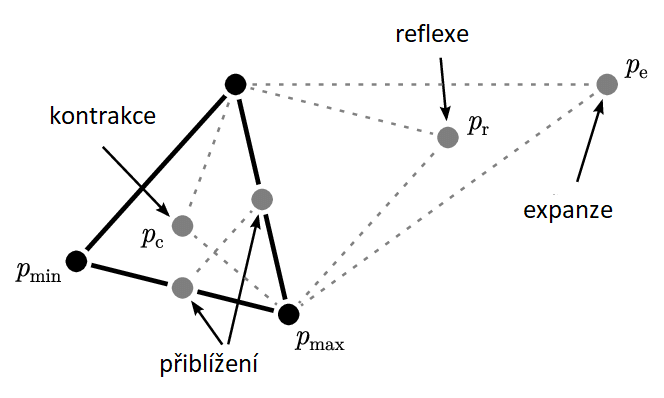
\includegraphics[width=0.8\textwidth]{obrazky-figures/nelderMead.png}
	\caption{Ukázka simplexu ve dvourozměrném prostoru a nelder-mead heuristik, které je možné nad tímto simplexem provést. Bod $p_{min}$ může být expandován na bod $p_e$, kontrakcí se z~něj stane centroid - bod $p_c$, reflexí bod $p_r$. Pokud ani jedna z~těchto operací nevylepší fitness hodnotu tohoto bodu v~prostoru, nastane operace přiblížení simplexu. Při této operaci je bod $p_{max}$ posunut na střed jedné ze sousedních hran, podle toho, která je lepším řešením. Body $p_{min}$ a $p_{max}$ označují (při minimalizaci) nejlepší a nejhorší bod v~rámci simplexu.}
	\label{fg:nm}
\end{figure}

\subsection{Řídící parametry a inicializace}
DE pracuje s~populací velikosti $N$, kde chromozom každého jedince je $D$-dimenzionální vektor $x_{i}$, kde $1 \leq i \leq N$ udává číslo jedince v~populaci. Velikost dimenze $D$ je dána dimenzí optimalizovaného problému. Dalšími parametry pro optimální fungování DE je \textit{faktor zesílení} $\beta$ a \textit{pravděpodobnost křížení} $CR$. Špatné zvolení těchto parametrů má detrimentální vliv na schopnost algoritmu nalézt optimum v~rozumném čase~\cite{Weisser2010}.
\begin{itemize}
    \item \textbf{Velikost populace} má přímý vliv na velikost prohledávaného prostoru. S~rostoucí velikostí populace roste pokrytí stavového prostoru, ale také časová složitost algoritmu. Empiricky bylo zjištěno, že velikost populace by měl být přibližně desetinásobek dimenze problému $D$ pro pokrytí celého stavového prostoru. Z~důvodu zrychlení konvergence algoritmu je ovšem častěji použit vztah $N \ge 2n_v + 1$, kde $n_v$ je parametrem selekčního schéma - počet diferenčních vektorů~\cite{Weisser2010}.
    \item \textbf{Faktor zesílení} určuje velikost mutace. Doporučená hodnota je $\beta = 0.5$. Příliš velká hodnota s~sebou přináší riziko přeskočení optima, zatímco příliš malá vede k~pomalé konvergenci a uváznutí. Velikost faktoru zesílení by měla být v~nepřímé úměře k~velikosti populace.
    \item \textbf{Pravděpodobnost křížení} má markantní vliv na diverzitu populace. Při operaci křížení určuje počet parametrů v~rámci jedince, které nebudou zděděny z~rodičovského vektoru. Velká hodnota vede na vysokou diverzitu a snížení schopností lokálního prohledávání prostoru~\cite{Weisser2010}.
    \item \textbf{Strategie} - poslední a velice důležitý parametr, určující jakým způsobem bude vytvářen vektor diferencí a jak bude probíhat křížení. Tato strategie je zapisována ve formátu $DE/x/y/z$, a platí že $x$ označuje způsob výběru bázového vektoru, $y$ počet vektorů pro výpočet vektoru diferencí a $z$ je typ křížení. Mezi nejpoužívanější (ovšem zdaleka ne jediné) strategie patří $DE/rand/1/bin$ nebo $DE/best/2/bin$~\cite{EVO}. Každá ze strategií s~sebou přináší výhody a nevýhody a jejich studium přesahuje rámec této práce. Pro zájemce doporučuji tento článek~\cite{DE_MUTATIONS}, který se této problematice věnuje.
\end{itemize}

Inicializace počáteční populace probíhá náhodně, pro každý parametr vždy v~rozmezí jeho definičního oboru.

\subsection{Mutace}
Mutace je v~kontextu DE chápána jako vytvoření tzv. vektoru diferencí (v~literatuře také šumový vektor) $\Vec{v_i}$, a je to základní stavební kámen celého algoritmu. Tento vektor slouží při křížení jako druhý rodič a způsob jeho vzniku je určen dříve zmíněným parametrem DE - strategie. Následující příklad popisuje vytvoření vektoru diferencí několika běžnými strategiemi~\cite{DE_IEEE, Weisser2010}. Parametr typu křížení nemá na generování mutací vliv a proto je zde vynechán.

\begin{itemize}
    \item \textbf{DE/rand/1} - šumový vektor je počítán ze tří náhodně vybraných jedinců z~aktuální populace. Váhovaný rozdíl (diference) mezi dvěma náhodně vybranými jedinci $\Vec{x_{r_2}}$ a $\Vec{x_{r_3}}$
    je připočten ke třetímu náhodnému jedinci $\Vec{x_{r_1}}$. Platí, že $r_1 \neq r_2 \neq r_3$. Graficky zobrazeno na obrázku~\ref{fg:de}. Rovnice tohoto vztahu:
    \begin{equation}
    \Vec{v_i} = \Vec{x_{r_1}} + \beta * (\Vec{x_{r_2}} - \Vec{x_{r_3}})
    \label{eq:de_rand_1}
    \end{equation} 

    \item \textbf{DE/rand/2} - modifikace $DE/rand/1/$. Vektor je počítán ze $4$ náhodných unikátních jedinců:
        \begin{equation}
    \Vec{v_i} = \Vec{x_{r_1}} + \beta * (\Vec{x_{r_2}} +\Vec{x_{r_3}} - \Vec{x_{r_4}} - \Vec{x_{r_5}})
    \label{eq:de_rand_2}
    \end{equation} 
    
    \item \textbf{DE/best/1} - je podobný $DE/rand/1/$; liší se pouze ve vektoru, ke kterému je připočítáván výsledek. V~této strategii se jedná o~$x_{best}$, tedy doposud nejlepší nalezený jedinec.
    \begin{equation}
    \Vec{v_i} = \Vec{x_{best}} + \beta * (\Vec{x_{r_2}} - \Vec{x_{r_3}})
    \label{eq:de_rand_1}
    \end{equation} 

    \item \textbf{DE/best/2} - analogicky k~$DE/rand/1$ a $DE/best/1$ vznikl $DE/best/2$ modifikací $DE/rand/2$.
    \begin{equation}
    \Vec{v_i} = \Vec{x_{best}} + \beta * (\Vec{x_{r_2}} +\Vec{x_{r_3}} - \Vec{x_{r_4}} - \Vec{x_{r_5}})
    \label{eq:de_rand_2}
    \end{equation} 
\end{itemize}

\noindent Jak je vidět, ve skutečnosti nic nebrání použití více než jednoho páru vektorů pro lineární kombinaci. Obecný tvar takové kombinace lze vyjádřit takto : 
 \begin{equation}
    \Vec{v_i} = \Vec{x_0} + \beta * \sum_{n=1}^{n_v}(\Vec{x_{r_{1}^{n}}} - \Vec{x_{r_{2}^{n}}})
    \label{eq:de_rand_2}
    \end{equation} 
kde $n_v$ bude počet dvojic vektorů, které si přejeme kombinovat a $x_0$ bude nějaký bázový vektor, který se liší od ostatních - nejlepší v~$best$ strategiích, náhodný v~$rand$~\cite{Weisser2010}.

Další známe strategie jsou~\cite{Weisser2010}:
\begin{itemize}
    \item \textbf{DE/current-to-best/$n_{v}$}, které pracuje s~momentálním řešením $i$ jako bázovým, ke kterému je připočítána váhovaná vzdálenost od nejlepšího $best$ spolu s~váhovanou vzdáleností dalších $n_v$ párů dvou náhodných unikátních $r_1$ a $r_2$.
     \begin{equation}
    \Vec{v_i} = \Vec{x_i} +  \beta * (\Vec{x_{best}} - \Vec{x_{i}}) + \beta * \sum_{n=1}^{n_v}(\Vec{x_{r_{1}^{n}}} - \Vec{x_{r_{2}^{n}}})
    \label{eq:de_rand_2}
    \end{equation} 
    \item \textbf{DE/rand-to-best/$n_{v}$}, které kombinuje přístup strategií $rand$ a $best$ - bázový vektor je poměr nejlepšího a náhodně vybraného vektoru udávaný náhodným parametrem $\gamma$.
     \begin{equation}
    \Vec{v_i} = \gamma * \Vec{x_{best}} + (1 - \gamma) * \Vec{x_{r_1}}  + \beta * \sum_{n=1}^{n_v}(\Vec{x_{r_{2}^{n}}} - \Vec{x_{r_{3}^{n}}})
    \label{eq:de_rand_2}
    \end{equation} 
    Opět zde platí, že náhodně generované vektory musí být unikátní a $0 \leq \gamma \leq 1$.
\end{itemize}


\subsection{Křížení a selekce}
Operace křížení následuje po vytvoření vektoru diferencí. Slouží k~vygenerování potomka - tzv. \textit{zkušebního vektoru} $x_{new}$~\cite{Weisser2010}. Ten je vytvořen za pomoci následujícího vztahu: 
     \begin{equation}
    \Vec{x_{new}}[k] = \begin{cases}
    \Vec{v_{i}}[k] & \text{ $N(0,1) \le CR$}\\
    \Vec{x_{i}}[k] &\text{jinak}
    \end{cases}
    \label{eq:de_rand_2}
    \end{equation} 
kde $\Vec{x_i[k]}$ je gen $k$ rodiče $\Vec{x_i}$, $\Vec{v_i[k]}$ je gen $k$ vektoru diferencí $\Vec{v_i}$ a $N(0,1)$ je náhodně vygenerované číslo od $0$ do $1$ normálním pravděpodobnostním rozložením.

Do nové populace je poté vybrán ten jedinec, který má lepší výsledky účelové funkce.

\begin{figure}[hbt]
	\centering
	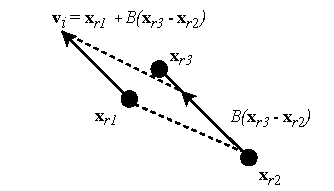
\includegraphics[width=0.8\textwidth]{obrazky-figures/de.pdf}
	\caption{Ukázka generování vektoru diferencí $v_i$ ve 2D prostoru strategií $DE/rand/1$. Převzato z~\cite{EVO}.}
	\label{fg:de}
\end{figure}

\section{Optimalizace hejnem částic}
\label{algs:pso}
Optimalizace hejnem částic~\cite{EVO}, anglicky Particle Swarm Optimization - PSO, je evoluční optimalizační technika inspirovaná pohybem zvířat v~hejnech, zejména ptáků. Bylo zjištěno, že schopnosti kolektivní spolupráce jedinců při vykonávaných činnostech (například hledání potravy) poskytuje těmto druhům evoluční výhodu. Metoda patří do skupiny zvané částicové systémy a od svého vzniku v~roce 1995 se pro tuto skupinu stala, společně s~metodou optimalizace mravenčí kolonií (ACO), hlavním představitelem. Na rozdíl od ACO, které je vhodnější spíše pro problémy diskrétního charakteru, je PSO navrženo pro problémy definované na spojité doméně. 

V~algoritmu je počet jednoduchých agentů - částic - umístěn do stavového prostoru optimalizovaného problému a každému z~nich je spočtena jeho fitness hodnota. Každý z~agentů poté spočítá svůj následující pohyb tak, že vezme v~potaz historii jeho vlastního pohybu, historii pohybu zbytku agentů v~hejnu a přidáním náhodné odchylky. Další iterace nastane poté, co se všechny částice pohnou na své nové pozice. Nakonec celé hejno, stejně jako hejno ptáků společně hledající jídlo, konverguje k~optimu~\cite{pso_article}. Princip zobrazen na obrázku~\ref{fg:pso_swarm}. 

Samotná částice by nebyla schopná nalézt optimum, jedná se o~emergentní vlastnost začlenění částic do společnosti a komunikovat. Tato společnost nemá vůdce ani žádnou centrální inteligence, přesto je schopna býti více než pouze součtem svých prvků.

\begin{definition} {Emergence\\}
Spontánní vznik makroskopických vlastností a struktur složitých systémů, jež není snadné odvodit z~vlastních jejich složek.
\label{def:emergence}
\end{definition}

\begin{figure}[hbt]
	\centering
	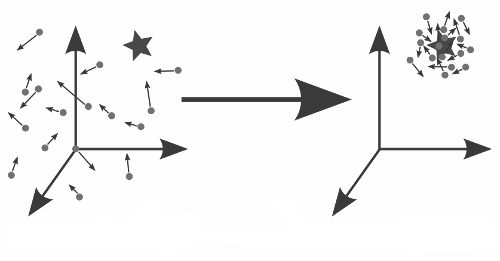
\includegraphics[width=0.8\textwidth]{obrazky-figures/pso.png}
	\caption{Vizualizace stavového prostoru s~částicemi na začátku (vlevo) a konci (vpravo) vykonávání PSO. Zdroj: internet.}
	\label{fg:pso_swarm}
\end{figure}

\subsection{Částice}
Každá částice v~hejnu se skládá ze tří D-dimenzionálních vektorů, kde $D$ je dimenze prohledávaného problému~\cite{pso_article}.
\begin{itemize}
    \item \textbf{Momentální pozice} \textbf{$\Vec{x}$.}
    \item \textbf{Dosavadní nejlepší pozice.} \textbf{$\Vec{p}$.}
    \item \textbf{Rychlost a směr pohybu.} \textbf{$\Vec{v}$.}
\end{itemize}
Momentální pozice je inicializována náhodnou hodnotou v~rámci stavového prostoru, dosavadní nejlepší pozice na zástupnou hodnotu, jejíž hodnota musí být horší než hodnota libovolného stavu ve stavovém prostoru. Rychlost a směr je inicializován náhodně ovšem v~rozumném rozmezí.


\subsection{Topologie}
Aby byla možná komunikace mezi jedinci, populace je uspořádána do jisté topologie~\cite{pso_article} - sociální sítě. Tuto síť si lze představit jako propojení dvou částic neorientovanou hranou, celou topologii si je poté možné představit jako neorientovaný graf. Částice má poté své \textit{sousedy}, kteří vytváří její \textit{sousedství} (nejedná se o~tranzitivní relaci). Toto rozdělení je důležité - částice ve stejném sousedství tíhnou k~prohledávání stejné oblasti. Každá částice objeví svou část prostoru a informuje o~tom sousedy. Ostatní částice o~této oblasti dostanou informaci až od svých sousedů - informační zpoždění. 

Originální PSO využívalo Euklidovského sousedství. To se ovšem prokázalo jako výpočetně náročná topologie s~nevhodnými konvergenčními vlastnostmi~\cite{pso_article}. V~současné době nejpoužívanější topologie jsou založeny na sociálním sousedství. Jedinci jsou sousedy bez ohledu na to, ve které části stavového prostoru se zrovna nacházejí. 

Typ sousedství se obecně rozděluje na dva druhy~\cite{pso_article}:

\begin{itemize}
    \item \textbf{Statická sousedství} - jak název napovídá, jedná se o~sousedství která se nemění v~průběhu vykonávání algoritmu. Typickým příkladem takového sousedství je tzv. \textit{gbest} -  úplná - topologie (obrázek~\ref{fg:pso_swarmTopo}). Dalším je \textit{lbest} topologie - kruh. Toto sousedství dovoluje paralelní prohledávání - rozdělení na regiony podle sousedství. Tato topologie konverguje pomaleji než gbest, ovšem lépe dokáže rozpoznat lokální optima a vyhnout se jim. Kompromisem mezi těmito topologiemi je \textit{von Neumann}, který dokáže kombinovat výhody obou. Obecně platí, že pro unimodální problémy jsou vhodnější gbest topologie, zatímco pro multimodální lbest.
    \item \textbf{Dynamická sousedství} - topologie měnící počet sousedů i sousedy samotné v~průběhu vykonávání algoritmu. Například uveďme techniku, při které se začíná s~lbest topologie pro podporu prohledávání a postupem času se přelíná do gbest pro podporu exploitace.
\end{itemize}


\begin{figure}[H]
	\centering
	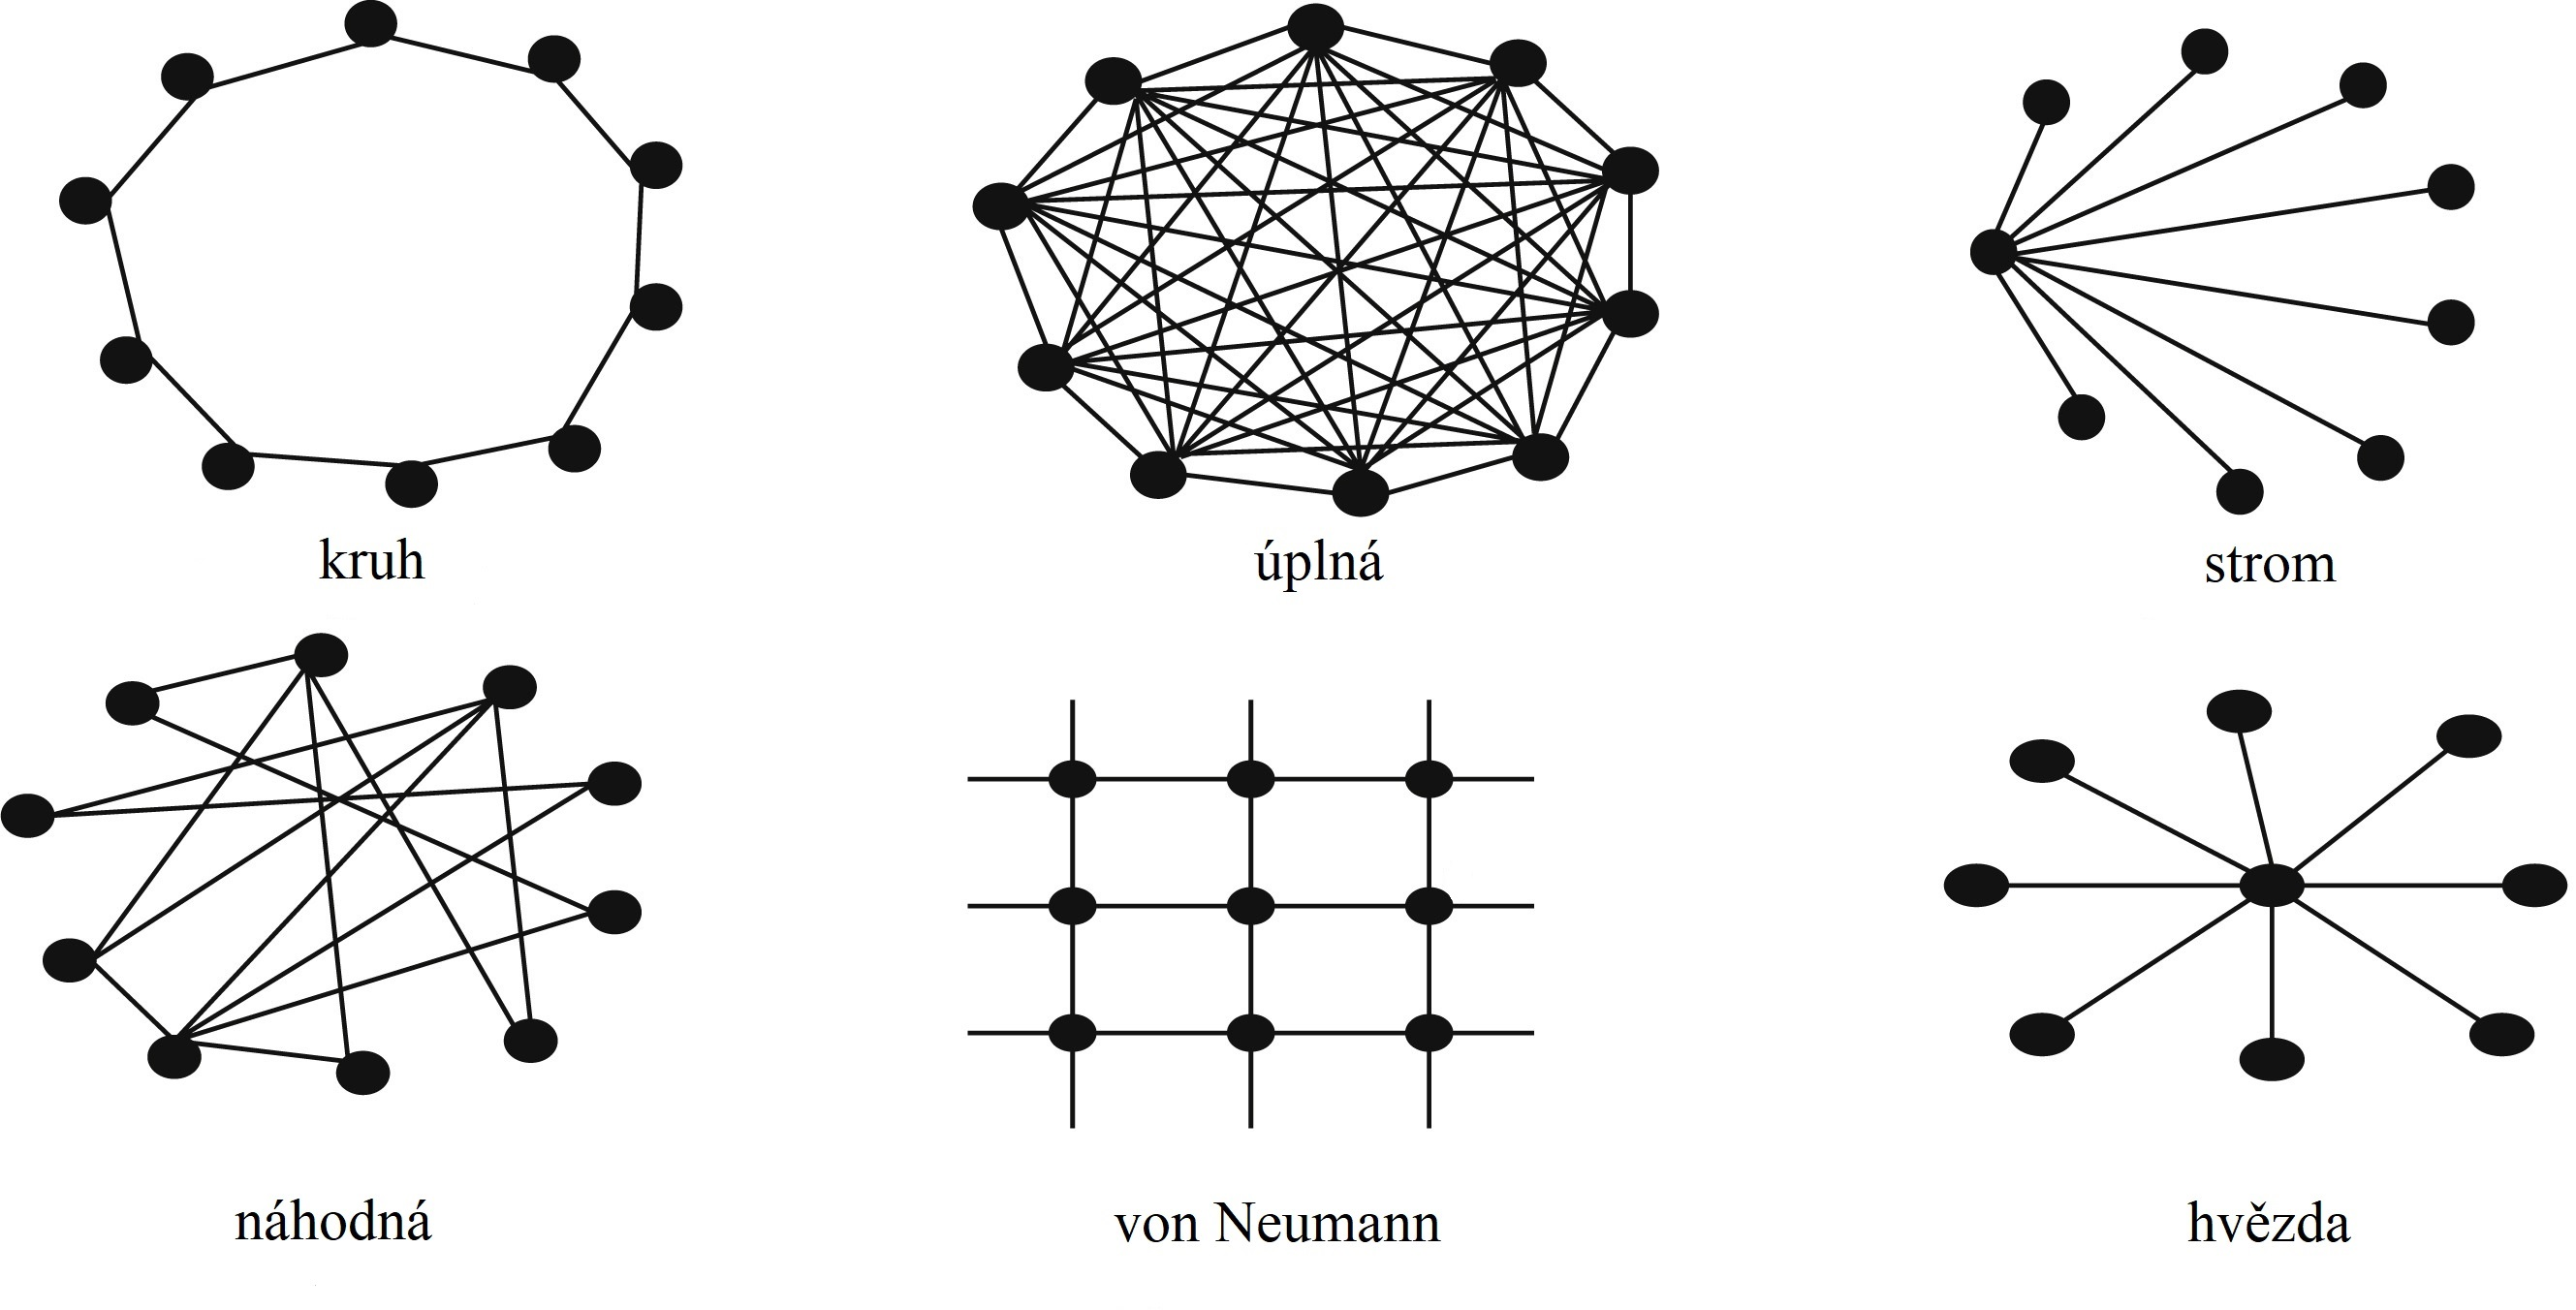
\includegraphics[width=0.6\textwidth]{obrazky-figures/psoTopo.jpg}
	\caption{Nejznámější PSO topologie.}
	\label{fg:pso_swarmTopo}
\end{figure}


\subsection{Výpočet směru}
 Nová pozice jedince je v~kanonickém PSO udána následující rovnicí~\cite{pso_article} (grafické znázornění je na obrázku~\ref{fg:pso_swarmProc}): 
    \begin{equation}
    \Vec{x_{i}}(g+1) = \Vec{x_{i}}(g) + \Vec{v_{i}}(g+1)
    \label{eq:pso1}
    \end{equation} 
kde $i$ udává jedince v~populaci, $\Vec{x_i}$ jeho pozici a $\Vec{v_i}$ jeho rychlost; $g$ je současná generace. Výpočet $\Vec{v_i}$ pro gen $j$ v~generaci $g$:

    \begin{equation}
    \Vec{v_{i}}[j](g+1) = \Vec{v_{i}}[j](g) + C_1 + C_2
        \label{eq:pso2}
    \end{equation} 
    
    \begin{equation}
     C_1 = c_1*N(0,1)* ( pBest_i[j](g) - \Vec{x_{i}}[j](g))
    \label{eq:pso3}
    \end{equation} 
    
    \begin{equation}
     C_2 = c_2*N(0,1)* ( gBest[j](g) - \Vec{x_{i}}[j](g))
    \label{eq:pso3}
    \end{equation} 
    

\begin{itemize}
    \item $pBest_i[j](g)$ je nejlepší nalezená pozice jedince $i$ pro gen $j$ v~generaci $g$.
    \item $gBest[j](g)$ je nejlepší nalezená pozice v~celém sousedství pro gen $j$ v~generaci $g$.
    \item $c_1$ a $c_2$ - akcelerační koeficienty.
    \item $N(0,1)$ - náhodně vygenerované číslo od $0$ do $1$ normálním pravděpodobnostním rozložením.
\end{itemize}


\begin{figure}[hbt]
	\centering
	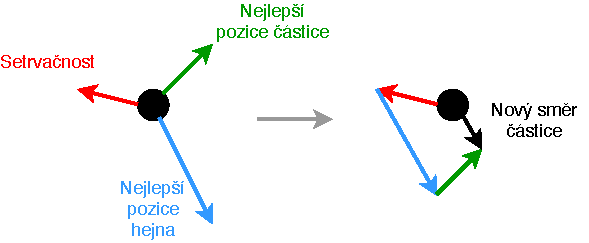
\includegraphics[width=0.8\textwidth]{obrazky-figures/pso2.pdf}
	\caption{Proces výpočtu následujícího směru pohybu částice. Dosavadní směr pohybu částice je přebit směrem pohybu hejna. Zdroj:~\cite{webPSO}.}
	\label{fg:pso_swarmProc}
\end{figure}



\subsection{Parametry}
PSO vyžaduje pro správné fungování nastavení při nejmenším následujících parametrů:

\subsubsection{Akcelerační koeficienty}
Koeficienty $c_1$ a $c_2$ určují, jak velkou váhu dává algoritmus nejlepším nalezeným pozicím agentem samotným ($pBest$ - $c_1$) a v~rámci sousedství ($gBest$ - $c_2$). Špatně nastavené koeficienty naruší rovnováhu prohledávání a vykořisťování a neumožní algoritmu konvergovat ke globálnímu optimu. Obecně se nastavuje $c_1 = c_2 = 2$ - částice přeletí optimum v~polovině případů. Čím vyšší je součet koeficientů, tím stoupá četnost oscilací kolem optima~\cite{pso_article}.

\subsubsection{Počet částic}
Vysoce závislé na typu problému, ovšem obecně se udává mezi 20 - 50 částicemi.

\subsubsection{Maximální rychlost částice}
Částicím je třeba omezit rychlost; při příliš velkých rychlostech by se mohlo stát, že částice bude provádět příliš velké kroky a optimum přeskakovat. Proto byla zaveden parametr $V_{max}$ a $V_{min}$, tedy minimální a maximální rychlost, kterou se může částice pohybovat. Dále se doporučuje, aby $V_{min} = - V_{max}$. V~případě, že částice povolenou rychlost překročí, je zastavena a je jí vygenerována nová náhodná rychlost ve stejném směru. I~zde je volba těchto parametrů závislá na problému, příliš nízká maximální rychlost omezuje prohledávání, zatímco příliš vysoká vykořisťování.



\subsection{Algoritmus}
Pseudokód algoritmu PSO vypadá následovně:

\begin{algorithm}[H]
\begin{algorithmic}
\State $InicializujHejnoCastic();$
\While{$! UkoncovaciPodminka()$}
\ForAll{$p \in Hejno$}
    \State $x = Pozice(p)$;
    \If{$Fitness(x) \leq Fitness(pBest(p)) $}
 	    \State $pBestUpdate(p, x)$
 	\EndIf
\EndFor
\State $gBestUpdate(pBest, Hejno)$
\ForAll{$p \in Hejno$}
     \State $VypocitejRychlostCastice(p)$
     \State $VypocitejPoziciCastice(p)$
\EndFor
\EndWhile
\State \Return $gBest;$
\end{algorithmic}
\caption{Optimalize hejnem částic}
\label{code:tabu}
\end{algorithm}

%%%%%%%%%%%%%%%%%%%%%%%%%%%%%%%%%%%%%%%%%%%%%%%%
\section{Evoluční strategie založená na adaptaci kovarianční \\\mbox{matice}}
\label{algs:cmaes}
Metoda známá pod zkratkou \uv{CMA-ES}, z~anglického \uv{Covariance Matrix Adaptation - Evolution Strategy}~\cite{CMAES}, je moderní state-of-the-art metoda pro optimalizaci v~doméně reálných čísel. Stejně jako ostatní EA, i ze je využíváno stochastických prvků. Základní kanonická verze \textit{evoluční strategie} využívá jako svůj hnací motor mutaci svých jedinců o~náhodnou hodnotu z~rozložení s~pevně danou směrodatnou odchylku $\sigma$. CMA-ES tento princip rozšiřuje použitím tzv. kovarianční matice, na základě které generuje nové jedince. Tato matice je neustále adaptována podle dosavadního stavu populace a umožňuje tak dynamicky upravovat velikost kroku a tím i prohledávaný stavový prostor. Tato adaptace poté udává tzv. cestu evoluce, kterou algoritmus používá k~učení a stanovení následujícího kroku směrem k~optimu. Algoritmus samotný nevyžaduje hluboké nastavování řídicích parametrů, což může být výhodou.

\subsection{Kovariance}
\label{ss:kovar}
Statistická charakteristika, určující míru lineární závislosti náhodných veličin $X$ a $Y$.
$$c(X,Y) = E[(X-E[X])*(Y-E[Y])]$$
kde $E[X]$ je střední hodnotou náhodné veličiny $X$.
\begin{itemize}
    \item $c(X,Y) > 0$ - veličiny se pohybují stejným směrem.
    \item $c(X,Y) < 0$ - veličiny se pohybují opačným směrem.
    \item $c(X,Y) = 0$ - veličiny jsou nezávislé.
\end{itemize}
Kovarianční matice $C$ pro $N$ proměnných je poté $N \times N$ matice, jejíž prvky jsou kovariance mezi proměnnými ($C_{ij}$ je spočtena jako $c(I,J)$). Na diagonále této matice je poté standardní odchylka náhodné veličiny $I$~\cite{CMAES}. Obecně lze vytvořit kovarianční matici pro libovolnou distribuční funkci, nejčastěji (jako i v~CMA-ES) se setkáme s~rozložením normálním.

\subsection{Adaptace}
Adaptace matice kovariancí zhruba odpovídá tzv. rekurzivní \textit{rank update} funkci. Jedná se o~přibližný, ovšem při vhodné volbě parametrů, dostatečně přesný odhad, abychom mohli považovat každou iteraci kovarianční matice za validní. Bylo zjištěno, že rank-one metoda je nejlepším estimátorem pro velké populace (obecně $\lambda/4 > 1 + \log n$)~\cite{CMAES}.

\subsubsection{Rank-One Update}
Základní operace nad maticí, odpovídající transformaci~\ref{eq:rankOneUpdate}. 
\begin{equation}
    A~+ \Vec{u}*\Vec{v}^T
    \label{eq:rankOneUpdate}
\end{equation}
kde $A$ je $K \times K$ matice a $u$ a $v$ dva $K \times 1$ vektory. Rank-One dostal svůj název kvůli hodnosti matice vzniklé vynásobením vektorů (matice hodnosti $1$).

Při adaptaci vypadá rank-one update následovně~\cite{CMAES}. Začínáme s~$m \in \mathbb{R}^n$, $C = \textbf{I}$, $\sigma = 1$, rychlost učení $c_{cov} \approx \frac{2}{n^2}$, $w_i$ je váha, která náleží vektoru $\Vec{y_i}$. Platí, že $\sum_{i=1}^{\mu}w_i = 1 $ a zároveň je $w_{i=1 \dots \lambda}$ nastaveno tak, aby platilo, že~\ref{eq:cmaes_muWeights} $\approx 0.4\lambda$. 
    \begin{subequations}
    \label{eq:cmaes}
    \begin{align}
        \Vec{x_i} &= \Vec{m} + \Vec{\sigma} \Vec{y_i}, \qquad \Vec{y_i} \sim N_i(\Vec{0}, C)  \label{eq:cmaes_sampling}\\
        \Vec{m} &\leftarrow \Vec{m} + \Vec{\sigma} \Vec{y_w}, \qquad \Vec{y_w} = \sum_{i=1}^{\mu}w_i\Vec{y_i} \label{eq:cmaes_mean}\\ 
        C &\leftarrow (1 - c_{cov})*C + c_{cov}* \mu_{w} * \underbrace{\Vec{y_{w}}\Vec{y_{w}}^{T}}_\text{rank-one}  \label{eq:cmaes_cUpdate} \\
        \mu_{w} &= \frac{1}{\sum_{i=0}^{\mu}w_{i}^{2}} \approx 0.4\lambda \label{eq:cmaes_muWeights} 
    \end{align}
    \label{eq:rankOne1}
    \end{subequations} 

V~těchto rovnicích je skryt téměř celý algoritmus CMA-ES. Zjednodušeně:
\begin{itemize}
    \item Je provedeno ohodnocení všech jedinců v~populaci, rovnice~\ref{eq:cmaes_sampling}.
    \item Je vybráno $\mu$ jedinců, jejichž váhová suma, společně se standardní odchylkou posouvá nový průměr příští generace. Přiřazování vah si lze představit jako selekční mechanismus tohoto algoritmu. Je nutno zmínit, že \textbf{je vybráno $\mu$ nejlepších řešení} (získáno fitness ohodnocením $\Vec{x_i}$), nikoliv náhodných. Rovnice~\ref{eq:cmaes_mean}.
    \item Za pomoci zmíněné sumy je adaptována kovarianční matice $C$.  Rovnice~\ref{eq:cmaes_cUpdate}.
\end{itemize}
\\
Adaptace matice způsobí, že CMA-ES~\cite{CMAES}
\begin{itemize}
    \item postupně zjistí všechny párové závislosti mezi proměnnými.
    \item provede analýzu hlavních komponent kroků $y_w$ tak, jak šli za sebou - rozložení na charakteristické vektory lineárních transformací kovarianční matice (rank update matice je symetrická, což zaručuje rozklad) - umožní rozpoznat libovolnou rotaci stavového prostoru proměnných a řešit takto rotovaný problém.
\end{itemize}
\\
a pokud je $\mu = 1$ poté je pro průměr nové generace vždy vybrán nejlepší jedinec v~populaci a CMA-ES provádí populační hill-climbing algoritus nad distribucí proměnných $N$.

Toto je v~krocích téměř celý algoritmus CMA-ES. Zásadní rozdíl mezi rovnicemi~\ref{eq:cmaes} a skutečným algoritmem je v~samotné adaptaci matice $C$. Pro její aktualizaci je ve skutečnosti vypočtena \emph{evoluční cesta}. Dále je třeba dát CMA-ES dříve zmíněnou dynamičnost postupnou úpravou standardní odchylky $\sigma$.

\subsubsection{Evoluční cesta}
Konceptuálně se jedná o~cestu, kterou se strategie vydala při hledání řešení. Znázorněno na obrázku~\ref{fg:evoPath}. Rekonstrukce této cesty se nazývá \textbf{kumulací} (nebo také například \uv{momentum} při fázi zpětné propagace umělých neuronových sítích - učení). Kumulace je v~CMA-ES spočtena dvakrát, tzv. \textbf{\uv{isotropická}}~\ref{eq:cmaes_po}, pro adaptaci zmíněné odchylky a~tím velikosti kroku algoritmu; a poté cesta \textbf{\uv{anisotropická}}~\ref{eq:cmaes_pc}. Tato cesta slouží k~adaptaci kovarianční matice a~směru, kterým se algoritmus vydá při zkoumání stavového prostoru~\cite{CMAES}. 


\begin{figure}[hbt]
	\centering
	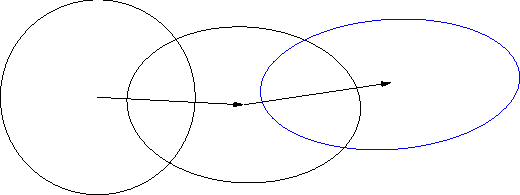
\includegraphics[width=0.65\textwidth]{obrazky-figures/evoPath.pdf}
	\caption{Názorná ukázka evoluční cesty. Elipsoidy znázorňují distribuční rozsah, tvar i střed je udán kovarianční maticí v~odpovídajícím kroku evoluce.}
	\label{fg:evoPath}
\end{figure}

Nechť $k$ označuje generaci
    \begin{subequations}
    \label{eq:cmaes}
    \begin{align}
        \Vec{p_\sigma}^{(k+1)} &\leftarrow (1 - c_{\sigma})\Vec{p_\sigma}^{k} + \sqrt{1 - (1 - c_{\sigma})^2} \sqrt{\mu_{w}}C^{-\frac{1}{2}}\Vec{y_w} \label{eq:cmaes_po}\\
        \Vec{p_c}^{(k+1)} &\leftarrow (1 - c_{c})\Vec{p_c}^{k} + h_{\sigma}*\sqrt{1 - (1 - c_{c})^2} \sqrt{\mu_{w}}\Vec{y_w} \label{eq:cmaes_pc}\\
        \mu_{w} &= \frac{1}{\sum_{i=0}^{\mu}w_{i}^{2}}, c_{cov} \ll c_c \approx c_{\sigma} \ll 1 \\
        h_{\sigma} &= 
        \begin{cases} 
            1       & pokud \quad \| p_{\sigma}\| < 1.5\sqrt{n}\\
            0       & jinak
        \end{cases}
    \end{align}
    \label{eq:pc}
    \end{subequations} 
\begin{itemize}
    \item $c_{c}$ a $c_{\sigma}$ jsou učící faktory pro anisotropickou a isotropickou cestu resp. Bylo ovšem zjištěno, že tyto hodnoty iterativně degradovaly přirozený rozptyl proměnných. Z~tohoto důvodu byly přidány normalizační výrazy (odmocnina $\sqrt{1-(1-c_{x})^2}$), které tento efekt zastavují (nastavením hodnot na 1 se z~rovnic vytratí i zmíněné mocniny).
    \item $C^{-\frac{1}{2}}$ - symmetrická odmocnina z~matice preciznosti (inverze kovarianční matice - obecně udává, jak moc je třeba transformovat originální data, aby byla nezávislá).
    \item $h_{\sigma}$ je zdržovací funkce. V~případě, že $\| p_{\sigma}\|$ je příliš vysoké, by docházelo k~příliš rychlému růstu elipsoidu daného maticí $C$ a tím i nechtěné diverzifikaci populace.
\end{itemize}


\subsubsection{Rank-$\mu$ update}
Pokud problém vyžaduje rychlou konvergenci (i za cenu globálního prohledávání), je třeba volit menší velikost populace. V~takovém případě ovšem již estimátor rank-one update není validní a je třeba využít jiné metodiky. Zde přichází na řadu \uv{Rank-$\mu$}. K~výpočtu následující kovariance je použita informace z~celé generace, na rozdíl od informace o~korelacích mezi generacemi.
\begin{subequation}
    \label{eq:rankMuC}
    \begin{align}
        C^{(k+1)} &= (1-c_{\mu}\sum w_i)C^k + c_{\mu}\sum_{i=1}^{\lambda}w_i \Vec{z_{i}}^{(k+1)}({\Vec{z_{i}}^{(k+1)}})^T \\
        z_{i}^{(k+1)} &= \frac{(y_{i}^{(k+1)} - m^k)}{\sigma_{i}^{k}}
    \end{align}
\end{subequation}

\subsection{Konečná podoba rovnic}
Kombinací rank-one a rank-$\mu$ metodik vzniká výsledná podoba adaptace kovarianční matice:
\begin{subequation}
    \label{eq:cmaes_rankMuC}
    \begin{align}
        C^{(k+1)} &\leftarrow (1-c_{cov}-c_{\mu}\sum w_i)C^k \nonumber \\ 
                &+ \underbrace{c_{cov}*\Vec{p_c}^{(k+1)}(\Vec{p_c}^{(k+1)})^T }_\text{rank-one} + \underbrace{c_{\mu}\sum_{i=1}^{\lambda}w_i \Vec{z_{i}}^{(k+1)}({\Vec{z_{i}}^{(k+1)}})^T}_\text{rank-$\mu$}
    \end{align}
\end{subequation}


\pagebreak
\noindent Přidáme-li i rovnici adaptace velikosti kroku $\sigma$, získáváme kompletní algoritmus \emph{CMA-ES}:

\begin{subequation}
\begin{gathered}
    \Vec{x_i} \leftarrow \Vec{m} + \Vec{\sigma} \Vec{y_i}, \qquad \Vec{y_i} \sim N_i(\Vec{0}, C)\vspace{4mm}\\
    sort(\Vec{y_i})\text{ podle hodnoty }f(\Vec{x_i})\\
    \Vec{m} \leftarrow \Vec{m} + \Vec{\sigma} \Vec{y_w}, \qquad \Vec{y_w} \leftarrow \sum_{i=1}^{\mu}w_i\Vec{y_i}\\ 
    \Vec{p_\sigma}^{(k+1)} \leftarrow (1 - c_{\sigma})\Vec{p_\sigma}^{k} + \sqrt{1 - (1 - c_{\sigma})^2} \sqrt{\mu_{w}}C^{-\frac{1}{2}}\Vec{y_w}\\
    \\
    \Vec{p_c}^{(k+1)} \leftarrow (1 - c_{c})\Vec{p_c}^{k} + h_{\sigma}*\sqrt{1 - (1 - c_{c})^2} \sqrt{\mu_{w}}\Vec{y_w}\\
    \\
    \mu_{w} \leftarrow \frac{1}{\sum_{i=0}^{\mu}w_{i}^{2}} \quad  h_{\sigma} \leftarrow 
        \begin{cases} 
            1       & \text{pokud} \quad \| p_{\sigma}\| < 1.5\sqrt{n}\\
            0       & \text{jinak}
        \end{cases}\\
        \\
        z_{i}^{(k+1)} = \frac{(y_{i}^{(k+1)} - m^k)}{\sigma_{i}^{k}}
        \\
        C^{(k+1)} \leftarrow (1-c_{cov}-c_{\mu}\sum w_i)*C^k \nonumber  + \underbrace{c_{cov}*\Vec{p_c}^{(k+1)}(\Vec{p_c}^{(k+1)})^T }_\text{rank-one} + \underbrace{c_{\mu}\sum_{i=1}^{\lambda}w_i \Vec{z_{i}}^{(k+1)}({\Vec{z_{i}}^{(k+1)}})^T}_\text{rank-$\mu$}\\
        \\
     \Vec{\sigma}^{(k+1)} \leftarrow  \Vec{\sigma}^{k} * \exp{\left(    \frac{c_{\sigma}}{1+\sqrt{\frac{\mu_w}{n}}}*\left[\frac{\|p_{\sigma}\|}{E\|N(\Vec{0}, \textbf{I})\|} - 1\right]\right)}
\end{gathered}
\end{subequation}
\\\\\\
\\
\\
\noindent
\begin{minipage}[t]{.33\textwidth}
Empiricky bylo zjištěno:
\begin{itemize}
    \item $\lambda \approx 4 + 3* \log N$ 
    \item $\mu \approx \frac{\lambda}{4}$
    \item $c_{cov} \approx \frac{2}{n^2}$
    \item $c_c \approx c_{\sigma} \approx \frac{4}{n}$
    \item $c_{\mu} \approx \min(\frac{\mu_w}{n^2}, 1-c_{cov})$
    \item $c_{cov} + c_{\mu} \le 1$
    \item $\sum w_i=\sum_{j=1}^{\lambda}w_j\approx\frac{-c_{cov}}{c_{\mu}}$
\end{itemize}
\end{minipage}
\hfill
\noindent
\begin{minipage}[t]{.32\textwidth}

Iniciální hodnoty:
\begin{itemize}
    \item $C = \textbf{I}$ 
    \item $p_c = \Vec{0}$
    \item $p_{\sigma} = \Vec{0}$
\end{itemize}
\end{minipage}
\begin{minipage}[t]{.32\textwidth}

Vstupy:
\begin{itemize}
    
    \item $\Vec{m} \in \mathbb{R}^n$ - počáteční průměrná hodnota 
    \item $\Vec{\sigma} \in \mathbb{R}_+$ - počáteční standardní odchylky jednotlivých proměnných
    \item $k_{max}$ - maximální počet generací
\end{itemize}
\end{minipage}

\chapter{Implementace a testování}
\label{impl}
Následující kapitola si nejprve klade za cíl představit vytvořený programový základ, který byl použit pro řešení problému hledání trajektorie sonikací. Následně představí několik běžných matematických funkcí pro testování optimalizačních metod, na kterých bude ověřena optimalizační schopnost vytvořeného řešení. Funkce nebyly vybrány náhodně, každá z~nich má odlišné vlastnosti a~testuje algoritmy podle jiných kritérií. V~poslední části budou prezentovány výsledky testovacích běhu, vedeny úvahy nad těmito výsledky a diskutována schopnost optimalizovat trajektorii sonikací \emph{HIFU}.
\section{Implementace}
Každý z~algoritmů představených v~kapitole~\ref{algs} byl implementován jako spustitelný optimalizér v~jazyce \emph{C++11} za pomoci externích knihoven \emph{GAUL}\footnote{\url{http://gaul.sourceforge.net/}} pro metody \emph{Genetického algoritmu}, \emph{Simulovaného žíhání}, \emph{Tabu prohledávání} a \emph{Diferenciální evoluce}, \emph{LibOPT}\footnote{\url{https://github.com/jppbsi/LibOPT}} pro metodu \emph{Optimalizace rojem částic} a \emph{CMA-ESpp}\footnote{\url{https://github.com/AlexanderFabisch/CMA-ESpp}} pro metodu \emph{CMA-ES}. Všechny tyto knihovny byly v~malé míře upraveny od jejich běžně dostupné varianty pro potřeby této práce. 

Dále vzniklo několik skriptů v~prostředí \emph{Bash} pro paralelní spuštění a sběr výsledků nezávislých optimalizací na clusterech \emph{IT4Innovation}. Skript v~jazyce \emph{Python3} pro generování relevantních statistických grafů z~těchto výsledků za pomoci balíčku \emph{MatplotLib}\footnote{\url{https://matplotlib.org/index.html}}. Pro překlad je poskytnut vzorový \texttt{Makefile} soubor. 

Implementované optimalizační programy a skripty pro kolekci dat vznikly pouze jako nezbytný nástroj pro potřeby této práce. Pro úpravy se předpokládá znalost programování, optimalizačních metod a alespoň mírná znalost rozhraní a datových struktur použitých externích knihoven. Všechen kód je řádně dokumentován v~doxygen komentářích ve zdrojových souborech.

\subsection{Sjednocení rozhraní externích knihoven}
Každá z~optimalizačních knihoven má výrazně odlišné rozhraní spuštění. Nastavení fitness funkce, podmínky konvergence a přerušení. I~výstupního protokol průběhových dat procesu optimalizace se výrazně liší. Z~toho důvodu bylo třeba vytvořit novou vrstvu mezi uživatelem a začátkem procesu optimalizace. Pro snadnou úpravu a jednotné spuštění procesu byl vytvořen modulární návrh využívající jednotných deklarací rozhraní v~hlavičkovém souboru. Tyto funkce jsou poté zakomponovány v~rámci unifikované mezivrstvy mezi spouštěnou aplikací a funkcí optimalizace externí knihovny. Samotná implementace metod je optimalizačnímu programu poskytnuta při linkovacím procesu v~průběhu překladu. Implementace nové fitness funkce je tedy možná definicí funkcí z~jednotného hlavičkového souboru a následné přilinkování tohoto souboru při překladu. Je nutné podotknout, že vzniklé optimalizační programy minimalizují.

\subsubsection{Modul fitness funkce}
Jak již bylo zmíněno, závazné deklarace pro implementaci nové účelové funkce jsou dostupné v~hlavičkovém souboru \texttt{FitnessFunction.h}. Soubor deklaruje následující funkce:
\begin{itemize}
    \item \verb|double fitnessFunction(int, double*)| pro výpočet fitness hodnoty. Funkce očekává na vstupu délku testovaného řešení a data ve formě ukazatele na typ double.
    \item \verb|int isInConstraints(int, double**)| pro ověření splnění omezujících podmínek. Pokud vstupní data splňují všechny uživatelem definované podmínky, funkce vrací $-1$, v~opačném případě pozici první proměnné, která omezení porušuje.
    \item \verb|void applyConstraints(int, double**)| pro aplikaci omezení a úpravu dat nalezeného řešení. I~zde je vstupem délka testovaného řešení a data tohoto řešení, které tato funkce může upravit. Tato funkce je vždy volána před funkcí ohodnocující fitness hodnotu řešení. Jedinou výjimkou je algoritmus CMA-ES, který tuto metodu nepoužívá.
    \item \verb|void getConstraints(int, double**, double**)| pro definici omezení stavového prostoru proměnných. Tato omezení jsou vrácena do optimalizace přes vstupní argumenty typu ukazatel na ukazatel na datový typ double. Jeden pro horní omezení, druhý pro spodní omezení. Funkce je zavolána před spuštěním optimalizace pro nastavení všech potřebných dat.
    \item \verb|bool isConverged(int, int, double, double, int, double**)| je volána na začátku každé generace pro kontrolu ukončovacích podmínek algoritmu. Vstupem metody jsou údaje o~počtu provedených generací, počtu evaluací fitness funkce, hledaná optimální fitness, nejlepší nalezená fitness, momentální velikost populace a fitness hodnoty celé dosavadní populace. Návratová hodnota indikuje, zda-li má být optimalizační proces ukončen.
\end{itemize}

\subsection{Mezivrstvy optimalizačních metod}
Samotný optimalizační algoritmus jednotlivých knihoven je volán z~mezivrstvy, která specializuje jednotné rozhraní účelové funkce na konkrétní požadavky externí knihovny. Tato vrstva je vstupním bodem každého vytvořeného programu.

\subsection*{GAUL optimalizační programy}
Knihovna \emph{GAUL - Genetic Algorightm Utility Library} je známou optimalizační knihovnou. Poskytuje několik běžně používaných optimalizačních algoritmu, z~nichž je v~této práci využito genetického algoritmu, simulovaného žíhání, tabu prohledávání a diferenciální evoluce. Zároveň je pro tyto metody (a nejvíce pro samotný genetický algoritmus) umožněna vysoká míra přizpůsobení - uživatel si může definovat vlastní genetické operátory. Toho bylo využito při implementaci mezivrstev zmíněných metod. Byl implementován vlastní operátor \texttt{randomUniformSeedInBounds(population*, entity*)} pro inicializaci populace. Tato inicializace respektuje omezeními pro každou z~dimenzí, namísto pouze jednoho globálního omezení, tak jak je to v~základu v~knihovně. Vstupní parametry jsou vnitřní datové struktury knihovny.

Dále vznikl mutační operátor \texttt{mutateDoubleMultipointCustomStddev(population*, entity*, entity*)}, který je schopen mutovat jedince v~populaci o~náhodně generované číslo z~normálního rozložení a vlastní standardní odchylkou, namísto standardních nabízených knihovnou, které mutují vždy s~odchylkou $1$. Tyto funkce se nachází v~souborech \texttt{CustomGaulFunctions.cc} a \texttt{CustomGaulFunctions.h}. Výpis textového výstupu a~předčasné ukončení obstarává funkce \texttt{generationHook(int, population*)}, případně \texttt{iterationHook(int, entity*)}. Knihovna maximalizuje, a funkce \texttt{scoreFunction(popu-\\lation*, entity*)} byla upravena adekvátně k~této skutečnosti. 
Vstupy pro spuštění optimalizace algoritmů z~knihovny GAUL jsou následující: 

\begin{itemize}
\item \textbf{Genetický algoritmus} -
v~implementované mezivrstvě je k~selekci použit \underline{turnaj}, křížení je prováděno \underline{dvoubodově} na náhodně vygenerovaných pozicích a mutace upravuje \underline{náhodný počet alel} za pomoci vlastního mutačního operátoru. Implementace této mezivrstvy se nachází v~souboru \texttt{GA\_Gaul.cc}. Pro spuštění optimalizace je nezbytné poskytnout následující hodnoty v~uvedeném pořadí:
\begin{itemize}
    \item maximální počet generací.
    \item velikost populace.
    \item dimenze problému.
    \item míra křížení - hodnoty $0$ až $1$.
    \item míra mutace - hodnoty $0$ až $1$.
    \item forma mezigeneračního přežití - celočíselné hodnoty $1$ až $3$ ($1$ - neudržuje se informace o~generaci, po vygenerování všech potomků jsou rodiče i děti seřazeny dle fitness a nejhorších $n$ je zabito, $2$ - lepší z~rodiče či dítěte je vybírán již při ohodnocení potomstva, $3$ - rodiče vždy umírají).
    \item optimální fitness - libovolné číslo z~$\mathbb{R}$.
    \item seed pro generátor náhodných čísel - libovolná posloupnost čísel.
    \item příznak, přejeme-li si výpis průběhu optimalizace.
\end{itemize}

\item \textbf{Simulované žíhání} - ke chlazení byl použit \underline{lineární rozvrh}, tedy v~každém kroku iterace je teplota snížena o~daný teplotní krok. Pro generování kandidátního řešení je využita perturberance, která posune každou hledanou proměnnou řešení o~náhodnou hodnotu. Tento náhodný posun je generován normálním rozložením s~průměrem $0$ a standardní odchylkou empiricky zvolenou na přibližně \textbf{$1/5$} rozmezí perturbované proměnné. I~zde je použit vlastní mutační operátor, popsaný na začátku sekce. Implementace mezivrstvy se nachází v~souboru \texttt{SA\_Gaul.cc}. Parametry spuštění v~uvedeném pořadí jsou následující:
\begin{itemize}
    \item maximální počet iterací.
    \item dimenze problému.
    \item počáteční teplota.
    \item teplotní krok.
    \item optimální fitness - libovolné číslo z~$\mathbb{R}$.
    \item seed pro generátor náhodných čísel - libovolná posloupnost čísel.
    \item příznak, přejeme-li si výpis průběhu optimalizace.
\end{itemize}

\item \textbf{{Tabu prohledávání}} - generování kandidátních řešení je zde provedeno stejnou metodou, jako u~simulovaného žíhání. Knihovna nepodporuje jinou, něž \underline{dlouhodobou paměť}. Zdrojovým souborem s~mezivrstvou je \texttt{Tabu\_Gaul.cc}. Pro spuštění optimalizace zakázaným prohledáváním je nutné poskytnout následující hodnoty v~uvedeném pořadí
\begin{itemize}
    \item maximální počet iterací.
    \item dimenze problému.
    \item délka tabu seznamu - maximální počet zakázaných stavů.
    \item počet testovaných kandidátních řešení.
    \item optimální fitness - libovolné číslo z~$\mathbb{R}$.
    \item seed pro generátor náhodných čísel - libovolná posloupnost čísel.
    \item příznak, přejeme-li si výpis průběhu optimalizace.
\end{itemize}

\item \textbf{{Diferenciální evoluce}} - knihovna GAUL nabízí $3$ níže uvedené strategie. Mezivrstva je implementována ve zdrojovém souboru \texttt{DE\_Gaul.cc}. Parametry spuštění v~uvedeném pořadí jsou tyto:
\begin{itemize}
    \item maximální počet generací.
    \item velikost populace.
    \item dimenze problému.
    \item počet generovaných diferenciálních vektorů.
    \item míra křížení - hodnoty $0$ až $1$.
    \item minimální faktor zesílení - libovolná kladná celočíselná hodnota.
    \item maximální faktor zesílení - hodnoty od minimálního faktoru dále.
    \item typ strategie - celočíselné hodnoty $1$ až $3$ ($1$ - strategie \emph{BEST}, $2$ - strategie \emph{RAND}, $3$ - strategie \emph{RAND-TO-BEST}).
    \item typ křížení - celočíselné hodnoty $1$ nebo $2$ ($1$ - křížení \emph{BIN}, $2$ - křížení \emph{EXP}).
    \item optimální fitness - libovolné číslo z~$\mathbb{R}$.
    \item seed pro generátor náhodných čísel - libovolná posloupnost čísel.
    \item příznak, přejeme-li si výpis průběhu optimalizace.
\end{itemize}
\end{itemize}

\subsection*{LibOpt optimalizační program}
Knihovna \emph{LibOpt} byla použita pro její realizaci optimalizace rojem částic. Pro využití této knihovny nebylo třeba příliš velkých úprav, pouze přizpůsobení rozhraní. Metoda využívá vlastních interních struktur \texttt{SearchSpace} a \texttt{Agent}. Stejně jako při GAUL optimalizačních programech, i zde byly implementovány funkce \texttt{scoreFunction(Agent*, ...)} a \texttt{generationHook(int, SearchSpace*)}, které plní stejné poslání. Knihovna minimalizuje.

\begin{itemize}
    \item \textbf{Optimalizace rojem částic} - knihovna poskytuje kanonickou verzi, která uvažuje \underline{jeden roj s~úplnou topologií}. Mezivrstva implementována souborem \texttt{PSO\_LibOpt.cc}. Pro spuštění optimalizace je nutné poskytnout následující hodnoty v~uvedeném pořadí
\begin{itemize}
    \item počet generací.
    \item počet částic.
    \item dimenze problému.
    \item akcelerační koeficient $c1$.
    \item akcelerační koeficient $c2$.
    \item faktor hybnosti.
    \item optimální fitness - libovolné číslo z~$\mathbb{R}$.
    \item seed pro generátor náhodných čísel - libovolná posloupnost čísel.
    \item příznak, přejeme-li si výpis průběhu optimalizace.
\end{itemize}
\end{itemize}

\subsection*{CmaESpp optimalizační program}
I~zde nebylo třeba větších úprav. Standardní funkce \texttt{scoreFunction(int, double*)} a \texttt{generationHook(CMAES)} jsou přítomny i zde. \texttt{CMAES} je interní datovou strukturou této knihovny. Dále byla přidána metoda, umožňující převzorkování jednotlivých genů, pro podporu hledání v~omezeném prostoru.
\emph{CmaESpp} je hlavičkovou knihovnou, což zjednodušilo sestavovací a linkovací proces. I~zde se jedná o~minimalizaci.

\begin{itemize}
    \item \textbf{CMA-ES} - mezivrstvu lze najít v~souboru \texttt{CMAES\_CmaESpp.cc}. Parametry spuštění v~uvedeném pořadí jsou následující:
\begin{itemize}
    \item maximální počet generací.
    \item dimenze problému.
    \item optimální fitness - libovolné číslo z~$\mathbb{R}$.
    \item seed pro generátor náhodných čísel - libovolná posloupnost čísel.
    \item příznak, přejeme-li si výpis průběhu optimalizace.
\end{itemize}
\noindent 
\end{itemize}
\subsection{Výstupní protokol}
Výstup každého z~optimalizačních algoritmů byl sjednocen. Text s~údaji je tištěn na standardní výstup a rozdělen do tří sekcí, oddělených posloupností symbolů \textbf{\texttt{"@@@"}}. Každá sekce se skládá z~posloupnosti dvojic \textbf{\texttt{klič:hodnota}}, kde jednotlivé dvojice jsou poté odděleny symbolem \textbf{\texttt{'\$'}} a libovolným počtem bílých znaků. V~případě, kdy \texttt{hodnota} je seznam, prvky tohoto seznamu jsou oddělený znakem \texttt{','}. Tento protokol byl zvolen, jelikož jej lze jednoduše převést do formátu \texttt{JSON}, čehož je následně využito ve skriptech generujících statistické grafy. Vzor pro ukázku struktury:

\begin{center}
\begin{tabular}{c}
\begin{lstlisting}[breaklines]
    $klíč:hodnota$klíč:hodnota$...$klíč:hodnota$
    @@@
    $klíč:hodnota$klíč:hodnota$...$klíč:hodnota1,hodnota2,...$
    $klíč:hodnota$klíč:hodnota$...$klíč:hodnota1,hodnota2,...$
    @@@
    $klíč:hodnota$klíč:hodnota$...$klíč:hodnota$
  
\end{lstlisting}
\end{tabular}
\end{center}
Obsah sekcí je následující:
\begin{itemize}
    \item První sekce je dedikována pro údaje o~spuštění. Zde se nachází všechny vstupní parametry, včetně omezení stavového prostoru.
    \item Druhá sekce obsahuje průběžné údaje o~prováděné optimalizaci (v~případě, že je výpis těchto údajů povolen při spuštění optimalizéru). Zde se, mimo jiné, nachází údaje o~nejlepším a nejhorším řešení v~populaci, statistická data o~populaci jako jsou kvartály, medián, průměr a dosavadní počet fitness vyhodnocení.
    \item V~poslední sekci jsou poté výsledky optimalizace. Nejlepší nalezená fitness, řešení a čas, po který optimalizace běžela.
\end{itemize}

Pro získání statistických dat vzniklo několik modulů, které jsou schopny extrahovat relevantní informace z~datových struktur jednotlivých knihoven. Tyto funkce jsou implementovány v~souborech \texttt{LoggingHooks\_[jméno knihovny].cc} a využity ve funkcích \texttt{iterationHook()}, případně \texttt{generationHook()}, která je volána vždy na začátku iterace, resp. generace.

\subsection{Skripty pro práci s~výsledky}
V~poslední řadě vznikly spolu s~optimalizačními programy i následující skripty:
\begin{itemize}
    \item \texttt{statsGenerator.py} - skript, který je schopen generovat statistické grafy z~textových výstupů několika běhů optimalizace. Grafy jsou generovány za pomoci knihovny \emph{matplotlib}. Veškeré výsledné grafy, které se nachází v~této a následující kapitole, byly generovány tímto souborem.
    \item \texttt{[opt]\_jobscript.pbs} - skripty pro systém PBS na clusterech \emph{IT4Innovation}. Umožňují automatizované masivní spuštění více běhů nezávislé optimalizace. Zkratka \textt{[opt]} představuje zkratku identifikující jednotlivé optimalizační metody - ga, sa, tabu, de, pso či cmaes.
    \item \texttt{paramOpt.py} - experimentální skript pro nalezení optimálních řídících parametrů jednotlivých optimalizačních metod za pomoci meta-optimalizace algoritmem Nelder-Mead. Ve finálním výsledku nebylo tohoto přístupu využito z~důvodu přílišné výpočetní náročnosti. Pro určení parametrů byl namísto toho zvolen empirický přístup.
\end{itemize}


\section{Sada testů}
\label{tests}
V~následující sekci bude představeno několik běžných matematických funkcí pro testování optimalizačních metod. Tyto funkce byly vybrány záměrně, každá z~nich má odlišné vlastnosti a testuje optimalizační algoritmus na jiné kritéria. Následně jsou ke každé funkci prezentovány statistické výsledky optimalizace provedené dříve představenými metodami. V~poslední části kapitoly budou zhodnoceny metody holisticky v~kontextu optimalizovaného systému \emph{HIFU}.

\subsection{Acleyho funkce}
První funkce v~testovací sadě je \textit{Acleyho funkce} - jedna z~snad o~nejznámější funkci pro testování optimalizačních metod. Je specifická svou podobou \textit{černé díře} - jedna hluboká propast ve středu funkce, ve které se nachází globální minimum, zatímco okolí této propasti je poseto lokálními minimy, ve kterých mohou optimalizační metody uváznout. Vizualizace ve dvou rozměrném prostoru je možné vidět na obrázcích~\ref{fg:acley} a~\ref{fg:acleyContour}. Funkční předpis:
\begin{equation}
f(\textbf{x}) = f(x_1, ..., x_n)= -a.exp(-b\sqrt{\frac{1}{n}\sum_{i=1}^{n}x_i^2})-exp(\frac{1}{n}\sum_{i=1}^{n}cos(cx_i))+ a + exp(1)
\label{eq:acley}
\end{equation}
Pro optimalizační účely jsou argumenty funkce omezeny intervalem $[-30, 30]$ a jejím globálním optimem je $f(0, \cdots, 0) = 0$. Konstanty $a$, $b$ a $c$ jsou běžně voleny jako $a = 20$, $b = 0.2$ a $c = 2\pi$

\begin{figure}[H]
	\centering
	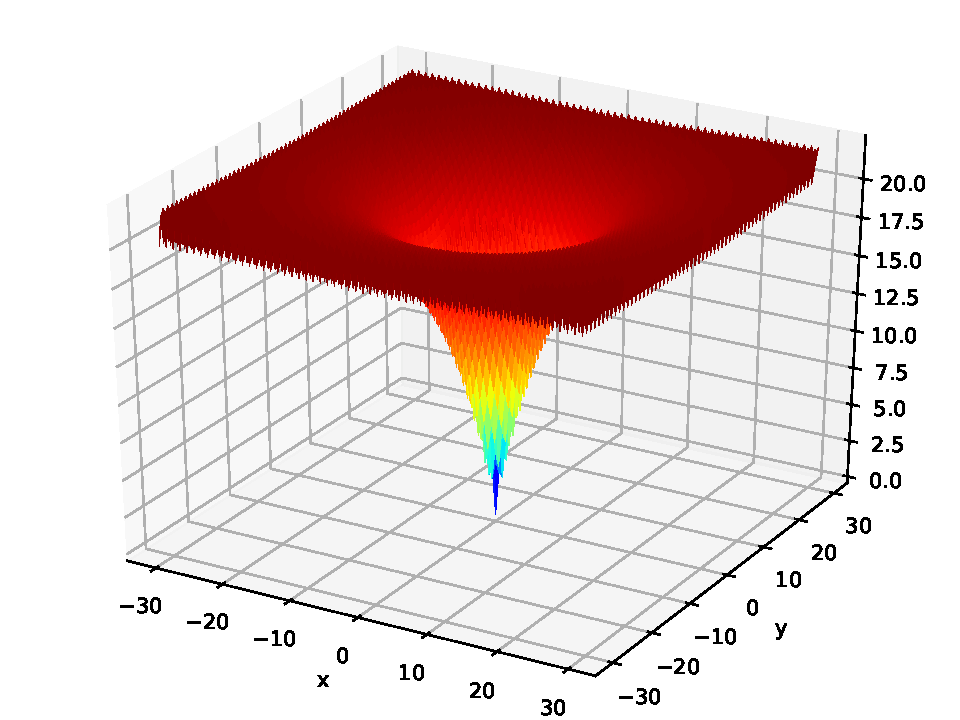
\includegraphics[width=0.7\textwidth]{obrazky-figures/ackley.pdf}
	\caption{Ackleyho funkce, vizualizace pro 2D.}
	\label{fg:acley}
\end{figure}
\begin{figure}[H]
	\centering
	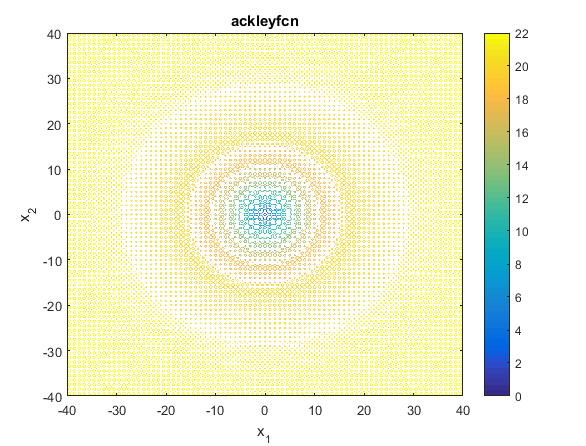
\includegraphics[width=0.7\textwidth]{obrazky-figures/ackleyfcn_contour.png}
	\caption{Ackleyho funkce, pohled na rovinu $x_1$,$x_2$.}
	\label{fg:acleyContour}
\end{figure}



\subsection{Griewankova funkce}
Další funkcí v~testovací sadě je \textit{Griewankova funkce} - jedna se o~funkci modelující šum. Celá funkce je poseta postupně se snižujícími lokálními minimy. Nejnižší z~nich se nachází ve středu; globální minimum. Tato funkce testuje především schopnost algoritmu prohledávat. Vizualizace ve dvou rozměrném prostoru je možné vidět na obrázcích~\ref{fg:griewank} a~\ref{fg:griewankContour}. Funkční předpis:
\begin{equation}
f(\textbf{x}) = f(x_1, ..., x_n) = 1 + \sum_{i=1}^{n} \frac{x_i^{2}}{4000} - \prod_{i=1}^{n}cos(\frac{x_i}{\sqrt{i}})
\label{eq:griew}
\end{equation}
Pro optimalizační účely jsou argumenty funkce omezeny intervalem $[-60, 60]$ a jejím globálním optimem je $f(0, \cdots, 0) = 0$.

\begin{figure}[H]
	\centering
	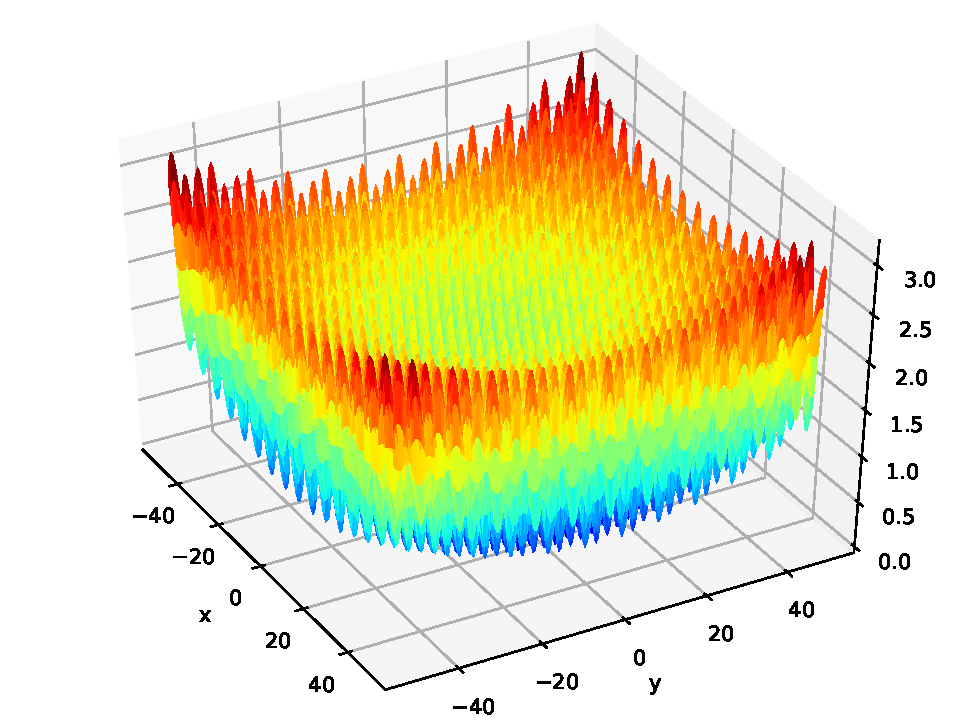
\includegraphics[width=0.7\textwidth]{obrazky-figures/griewank.pdf}
	\caption{Griewankova funkce, vizualizace pro 2D.}
	\label{fg:griewank}
\end{figure}

\begin{figure}[H]
	\centering
	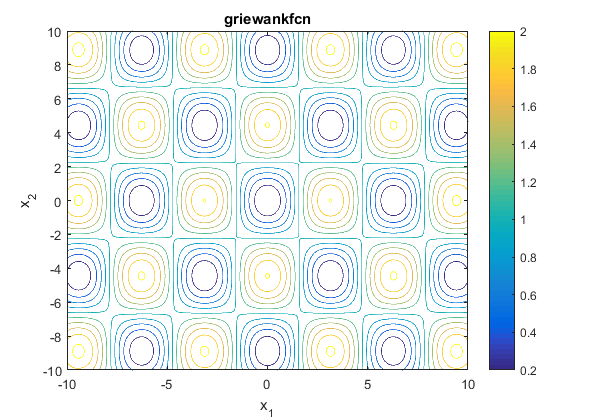
\includegraphics[width=0.7\textwidth]{obrazky-figures/griewankfcn_10_contour.png}
	\caption{Griewankova funkce, pohled na rovinu $x_1$,$x_2$.}
	\label{fg:griewankContour}
\end{figure}

\begin{figure}[H]
	\centering
	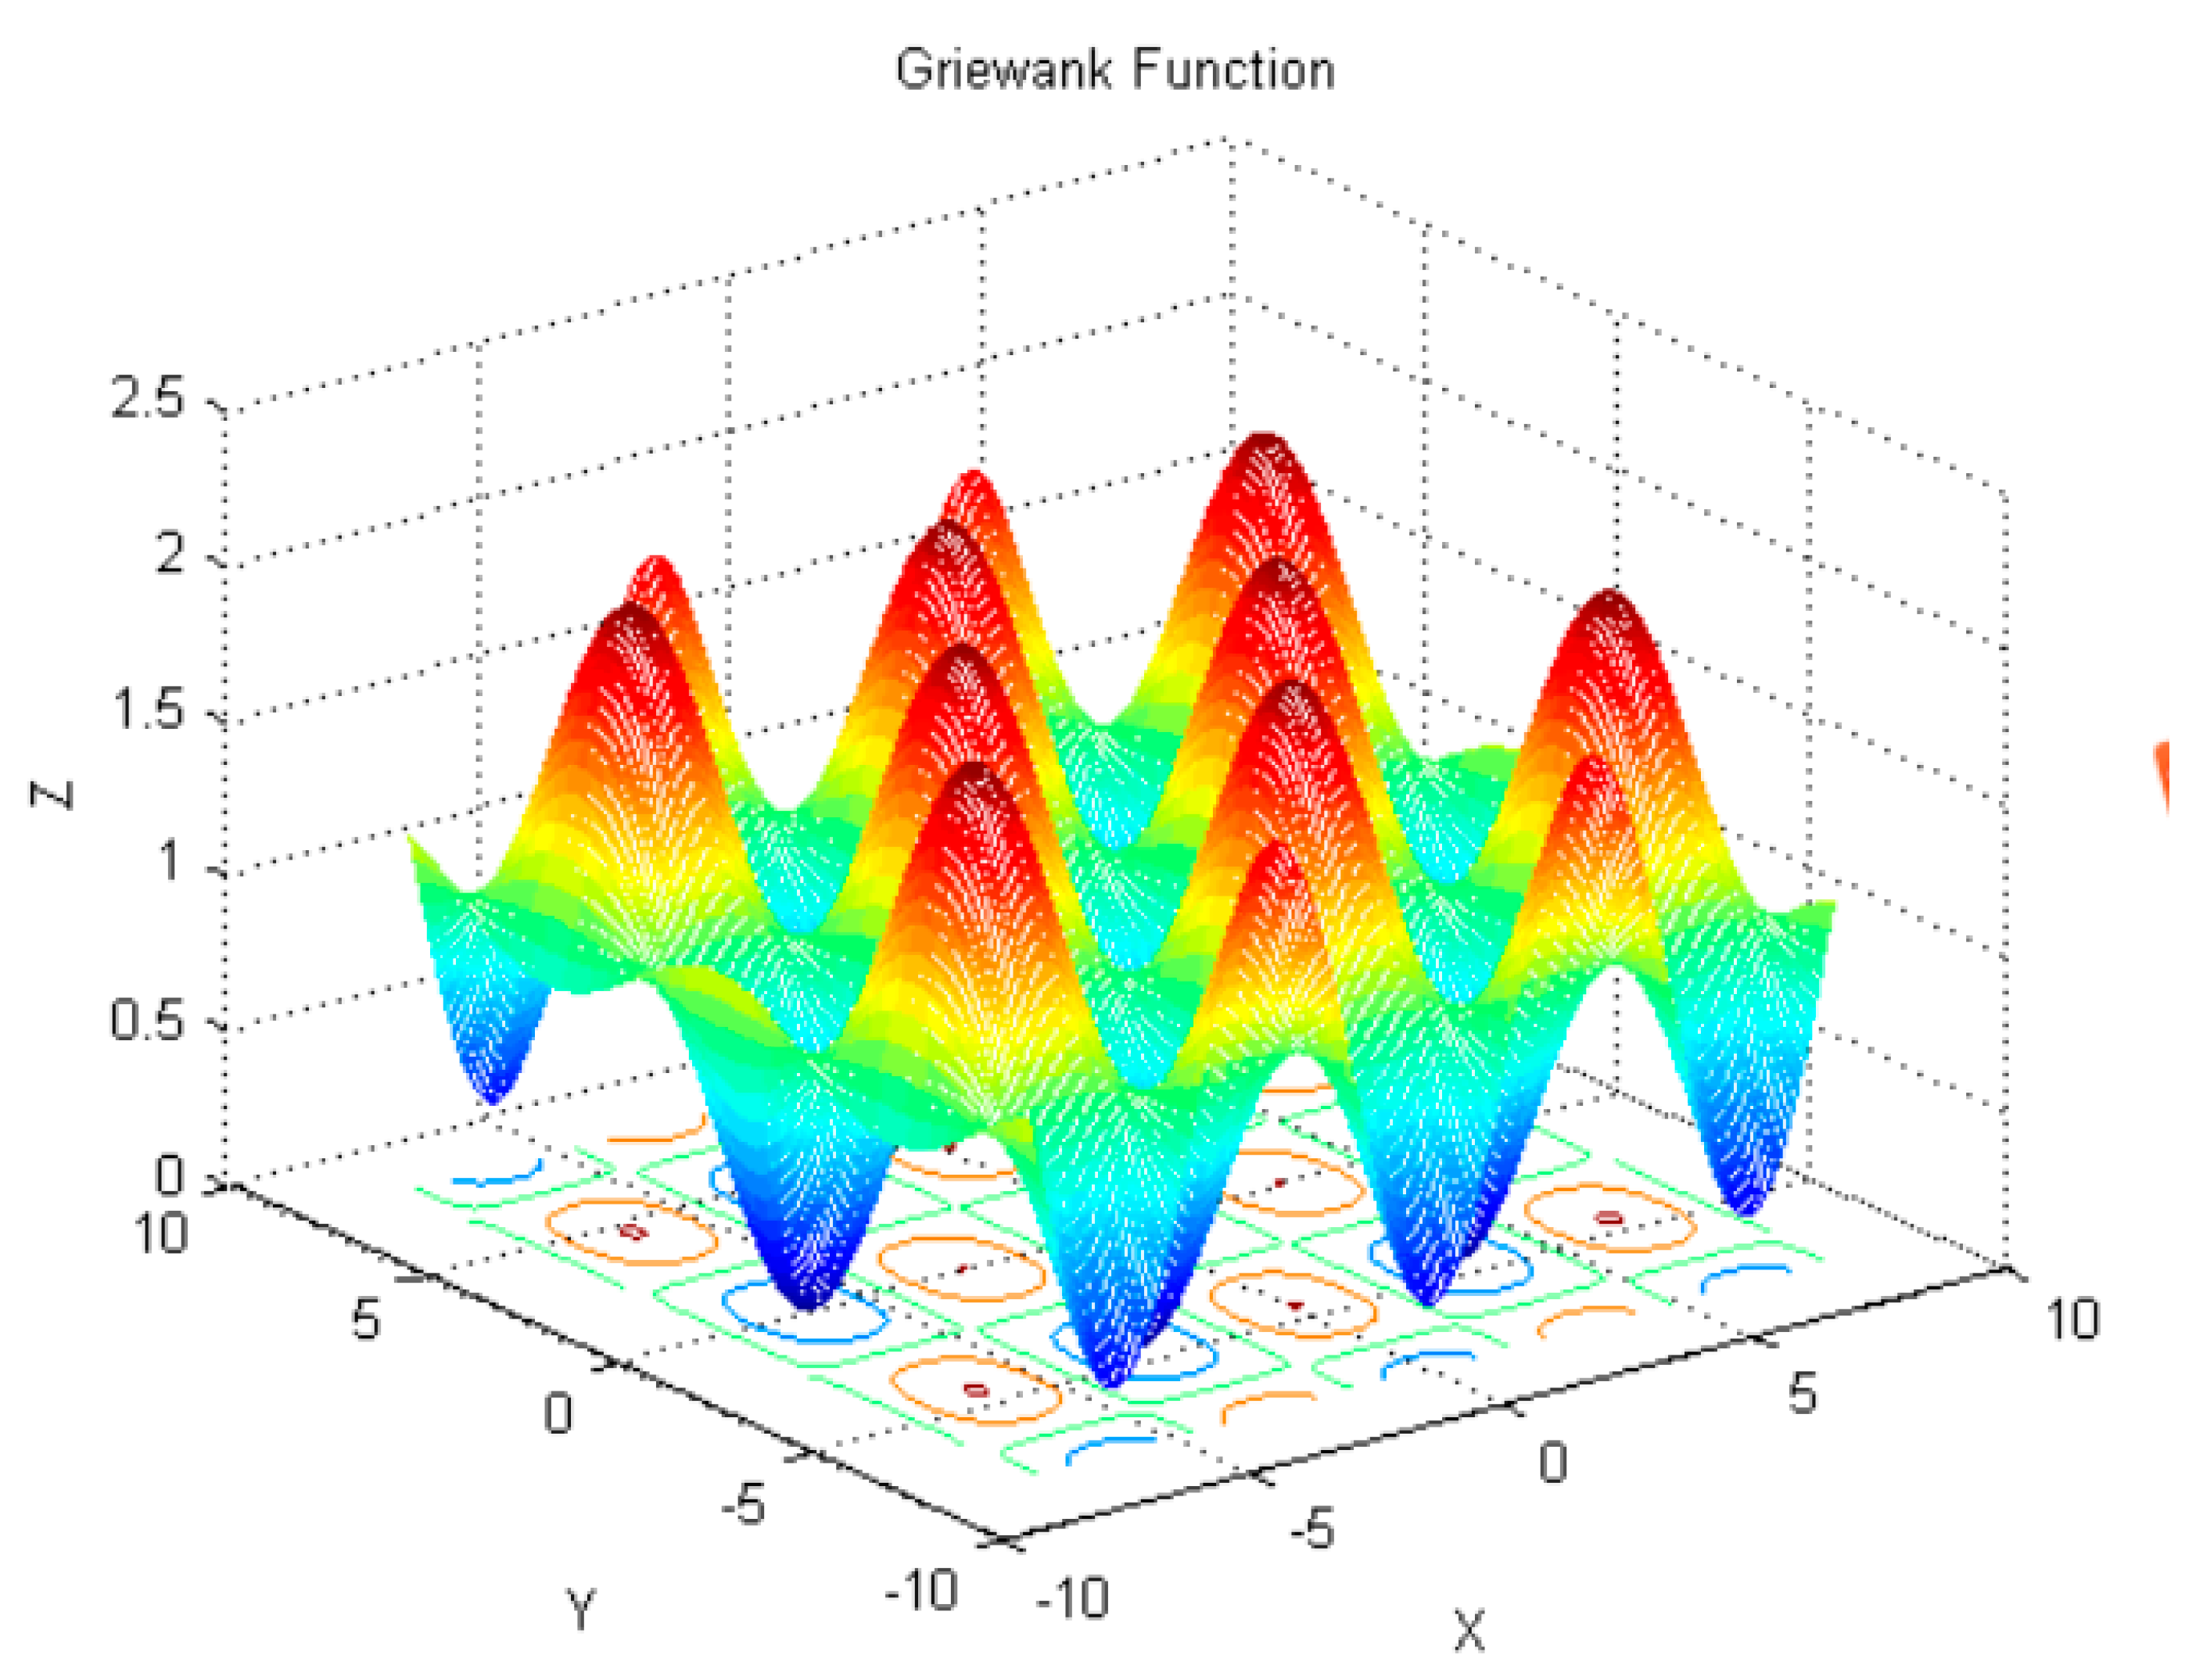
\includegraphics[width=0.7\textwidth]{obrazky-figures/griewank_zoom.png}
	\caption{Griewankova funkce, náhled na okolí optima.}
	\label{fg:griewankZoom}
\end{figure}



\subsection{Rosenbrockova funkce}
Poslední v~testovací sadě je \textit{Rosenbrockova funkce}, označována také za \uv{banánovou} funkci. Jedná se o~jednu z~nejpoužívanějších funkcí pro testování optimalizačních algoritmů. Funkce je unimodální, její globální minimum leží v~úzkém, parabolickém údolí. Toto údolí je většinou jednoduché najít, funkce testuje spíše schopnost metod konvergovat k~minimu. Vizualizace ve dvou rozměrném prostoru je možné vidět na obrázcích~\ref{fg:rosen} a~\ref{fg:rosenContour}. Funkční předpis:
\begin{equation}
f(\Vec{x}) = \sum_{i=1}^{d-1}[ 100*(x_{i+1} - x_{i}^2)^{2} + (x_{i} - 1)^{2}]
\label{eq:boha}
\end{equation}
Pro optimalizační účely jsou argumenty funkce omezeny intervalem $[-5, 10]$ a jejím globálním optimem je $f(1, \cdots, 1) = 0$.


\begin{figure}[H]
	\centering
	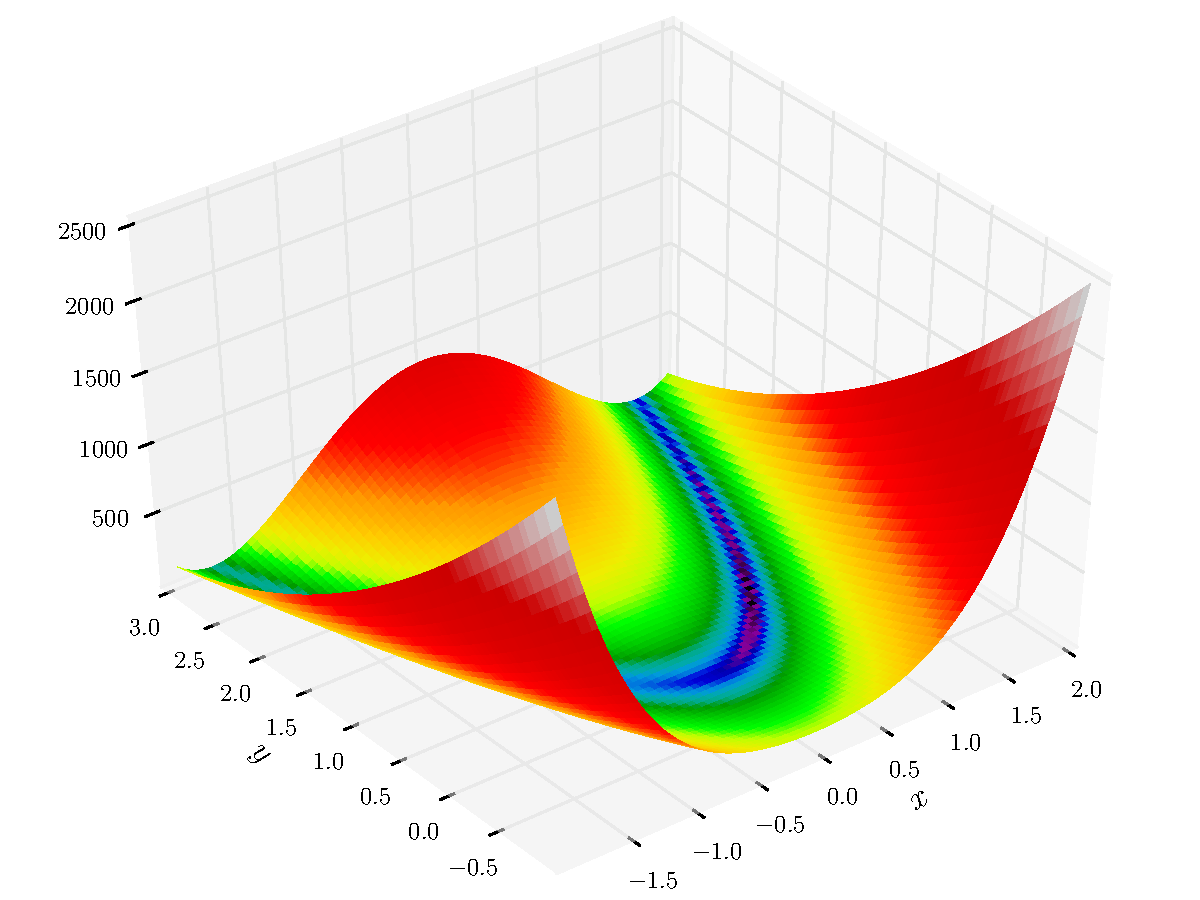
\includegraphics[width=0.7\textwidth]{obrazky-figures/rosenbrock.pdf}
	\caption{Rosenbrockova funkce, vizualizace pro 2D.}
	\label{fg:rosen}
\end{figure}
\begin{figure}[H]
	\centering
	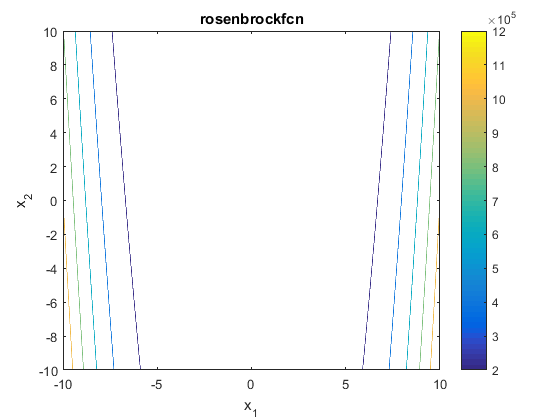
\includegraphics[width=0.7\textwidth]{obrazky-figures/rosenbrockfcn_contour.png}
	\caption{Rosenbrockova funkce, pohled na rovinu $x_1$,$x_2$.}
	\label{fg:rosenContour}
\end{figure}

%%%%%%%%%%
\section{Testování}
Následující sekce prezentuje výsledky optimalizace představené testovací sady. Nejprve je sada použita pro validaci jednotlivých implementovaných metod a následně jsou experimenty provedeny znovu, tentokrát s~ohledem na vybraná kritéria. V~poslední části jsou diskutovány výsledky těchto omezených běhů a přínos pro cíl této práce.
\subsection{Parametry spuštění}
V~předešle kapitole bylo nastíněno, že jedním z~hlavních problémů, které je třeba vyřešit při použití evolučních metod, je vhodné nastavení řídicích parametrů. K~tomu je třeba znalost metody i konkrétního optimalizovaného problému. V~případech, kdy je problém typu \emph{black-box} se dostáváme do situace, ve které je třeba experimentovat a parametry určit empiricky nebo za pomoci meta-optimalizačních technik. Tato technika popisuje využít další, nadřazené optimalizační metody (jsou typicky voleny ty, které nejsou na řídicí parametry příliš citlivé) pro nalezení vhodných parametrů. Tento přístup má svou stinnou stránku - počet vyhodnocení fitness funkce roste exponenciálně. Tohoto přístupu si ovšem práce nemůže dovolit. Vyhodnocení simulace šíření tepla je velice výpočetně náročné a extenzivně experimentovat, či využít jiných strojových metodik pro nalezení řídicích parametrů si nemůžeme dovolit. Z~tohoto důvodu si tato sekce klade za cíl i nalezení jisté vhodné \emph{redukce} tohoto modelu na některou (či kombinaci některých) z~testovacích funkcí. Odpovídající funkci můžeme považovat za formu aproximace a úvodní řídící parametry nastavit podle poznatků o~této metodě.

\subsection{Kritéria hodnocení}
Snahou práce je ovšem nalézt vhodný algoritmus pro optimalizaci systému HIFU (prezentován v~kapitole~\ref{about}). Pro tento cíl je nutné navrhnout kritéria, podle kterých budeme algoritmy posuzovat. Jak již bylo nastíněno, tyto kritéria musí vyjadřovat poměr mezi počtem evaluací simulace šíření tepla ve tkáních a přesností nalezení trajektorie. Tyto kritéria jsou reprezentována zavedeným omezením optimalizace na maximálně $2000$ vyhodnocení účelové funkce a tím i evaluací simulace (obecně jedna simulace se skládá z~provedení $n$ sonikací). Toto omezení se na první pohled může zdát relativně přísné, ovšem je třeba zvážit situaci. Pacient čekající na odstranění zhoubného nádoru si nemůže dovolit dlouho čekat, samotná simulace je přizpůsobena jeho případu, který se každým dnem vyvíjí. Zhoubná tkáň se den za dnem rozšiřuje, mění tvar nebo i otáčí a i malá změna znehodnotí nalezené výsledky. A~přesto, že jednomu vyhodnocení simulace nelze přiřadit časovou hodnotu - je vysoce závislá na počtu sonikací a i parametrech samotné sonikace, je třeba se pokusit o~včasnost výsledku. $2000$ je čistě empirická hodnota - jedná se o~$8$ hodin výpočtu $20$ sonikací pro relativně průměrné hodnoty dob pálení a čekáni. Výpočty byly navíc prováděny na clusterech $IT4Innovation$, což jsou vysoce výkonné výpočetní zařízení, na kterých je možné uplatnit masivního paralelizmu.

V~ideálním případě by pro minimalizaci rizika zranění pacienta hrálo roli i nezbytný počet sonikací. Toto je ovšem problém, jehož řešení se může výrazně lišit model od modelu a jakékoliv nalezení řešení pro jednu specifickou situaci nelze považovat za obecně odpovídající. Cílem je proto nalézt takový algoritmus, který zvládá nízké i vysoké počty sonikací. 

\subsection{Testy}
Nejprve byla pro ověření validity nastavena dimenze problému na $\textbf{5}$ proměnných bez dodatečných omezení. Výsledky této validace lze vidět v~přílohách na obrázcích~\ref{fg:validation:ackley:joined},~\ref{fg:validation:griewank:joined} a~\ref{fg:validation:rosenbrock:joined}. Následně byly testy provedeny znovu, tentokrát s~omezením na $2000$ evaluací účelové funkce a dimenzí problému nastavenou na $16$. Tato omezení odpovídají hledání trajektorie o~$4$ sonikacích. Běžně se při HIFU operacích používají desítky, $4$ slouží pouze pro ověření konceptu.


\pagebreak
\subsubsection*{Ackleyho funkce}
\label{subsub:ackley:res}
Následující výsledky jsou agregací 30 běhu každého algoritmu. Parametry spuštění byly následující:
\\
\begin{table}[H]
\centering
\resizebox{\textwidth}{!}{%
\begin{tabular}{|c|c|c|c|c|c|}
\hline
\multirow{3}{*}{\textbf{GA}} &
  \multirow{3}{*}{\begin{tabular}[c]{@{}c@{}}64 jedinců \\ v~populaci\end{tabular}} &
  \multirow{3}{*}{\begin{tabular}[c]{@{}c@{}}Turnajový \\ výběr\end{tabular}} &
  \multirow{3}{*}{\begin{tabular}[c]{@{}c@{}}Dvoubodové \\ křížení 80\%\end{tabular}} &
  \multirow{3}{*}{\begin{tabular}[c]{@{}c@{}}Mutace \\ 15\%\end{tabular}} &
  \multirow{3}{*}{\begin{tabular}[c]{@{}c@{}}Přežití nejlepších \\ bez ohledu \\ na generaci\end{tabular}} \\
 &
   &
   &
   &
   &
   \\
 &
   &
   &
   &
   &
   \\ \hline
\multirow{2}{*}{\textbf{SA}} &
  \multirow{2}{*}{\begin{tabular}[c]{@{}c@{}}Počáteční \\ teplota 2000\end{tabular}} &
  \multirow{2}{*}{Krok 1\%} &
  \multicolumn{3}{c|}{\multirow{2}{*}{Lineární chladící rozvrh}} \\
 &
   &
   &
  \multicolumn{3}{c|}{} \\ \hline
\textbf{Tabu} &
  \begin{tabular}[c]{@{}c@{}}20 prvků \\ v~tabu seznamu\end{tabular} &
  \multicolumn{4}{c|}{5 kandidátních řešení} \\ \hline
\textbf{DE} &
  \begin{tabular}[c]{@{}c@{}}40 jedinců \\ v~populaci\end{tabular} &
  \begin{tabular}[c]{@{}c@{}}Strategie \\ BEST/1/BIN\end{tabular} &
  \begin{tabular}[c]{@{}c@{}}Šance rekombinace \\ 80\%\end{tabular} &
  \multicolumn{2}{c|}{\begin{tabular}[c]{@{}c@{}}Faktor zesílení \\ 0.5 až 0.9\end{tabular}} \\ \hline
\textbf{PSO} &
  100 částic &
  \multicolumn{2}{c|}{\begin{tabular}[c]{@{}c@{}}Akcelerační koeficienty \\ c1 = c2 = 2\end{tabular}} &
  \multicolumn{2}{c|}{\begin{tabular}[c]{@{}c@{}}Koeficient \\ setrvačnosti 0.5\end{tabular}} \\ \hline
\textbf{\begin{tabular}[c]{@{}c@{}}CMA\\   ES\end{tabular}} &
  \multicolumn{5}{c|}{\textit{Nevyžaduje vstupní parametry.}} \\ \hline
\end{tabular}%
}
\label{tb:bench:ackley}
\caption{Řídící parametry jednotlivých optimalizačních metod pro omezenou optimalizaci Ackleyho funkce.}
\end{table}
Výsledky je možné vidět na grafech~\ref{fg:bench:ackley:joined} a~\ref{fg:bench:ackley:cmaes}. Je patrné, že až na \emph{CMA-ES} nebyl žádný z~algoritmů schopen dosáhnout skutečného optima. Zastavili se v~jednom z~mnohých lokálních extrémů při strmém sestupu a nedokázali jej překonat. Nejhůře dopadl genetický algoritmus, což není příliš překvapující; $2000$ vyhodnocení účelové funkce je obecně pro populačně založené algoritmy málo. Genetické algoritmy typicky vyžadují mnohonásobně vyšší počet vyhodnocení k~dosažení optima. Z~grafu posledních generací (přílohy, graf~\ref{fg:bench:ackley:ga:lastGen}) je možné vidět, že populace si nebyly schopny udržet diverzitu. Za zmínku stojí také metoda diferenciální evoluce, která se zdá být zdravá (grafy~\ref{fg:bench:ackley:de:evoProg}) a jednoduše nestihla dokončit evoluci. 

\begin{figure}[H]
\makebox[\textwidth][c]{
    \begin{tabular}{cc}
	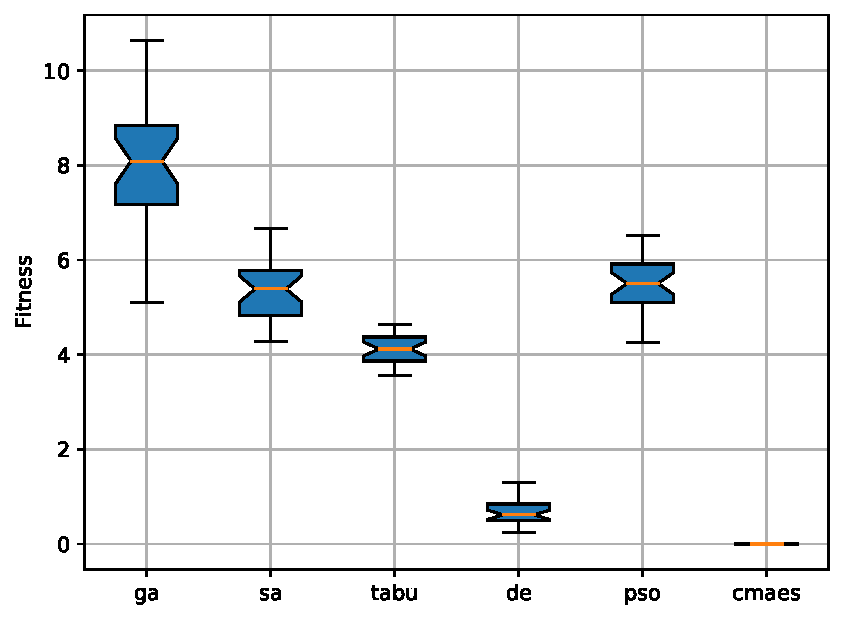
\includegraphics[width=75mm]{obrazky-figures/statistics/Benchmarks/Ackley/JOINED/solutionsPlotsComparasion.pdf}
    &
	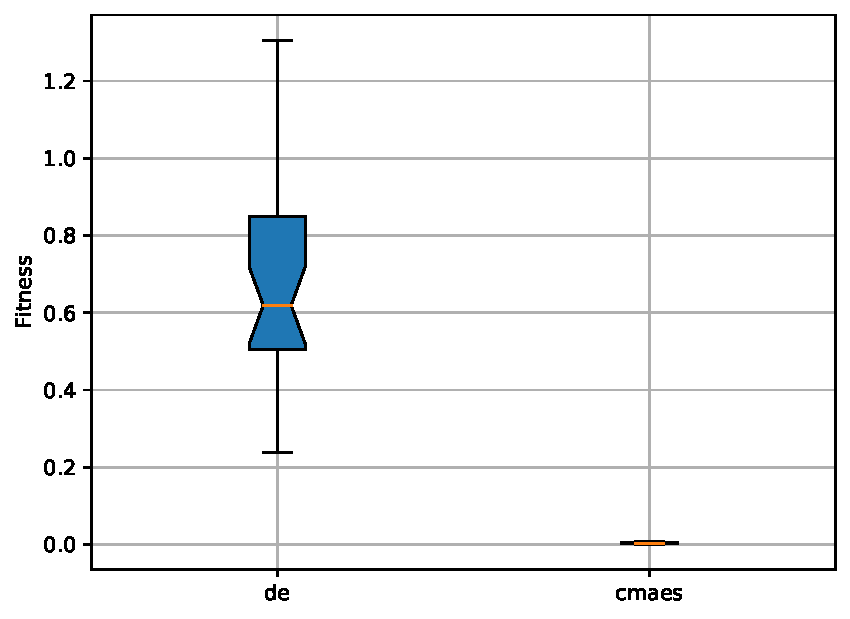
\includegraphics[width=75mm]{obrazky-figures/statistics/Benchmarks/Ackley/JOINED/detail_solutionsPlotsComparasion.pdf}
    \end{tabular}
    }
    \caption{Výsledky omezené optimalizace Ackleyho funkce. Vlevo všechny algoritmy, vpravo detail na diferenciální evoluci a CMA-ES.}
    \label{fg:bench:ackley:joined}
\end{figure}

\begin{figure}[H]
    \centering
	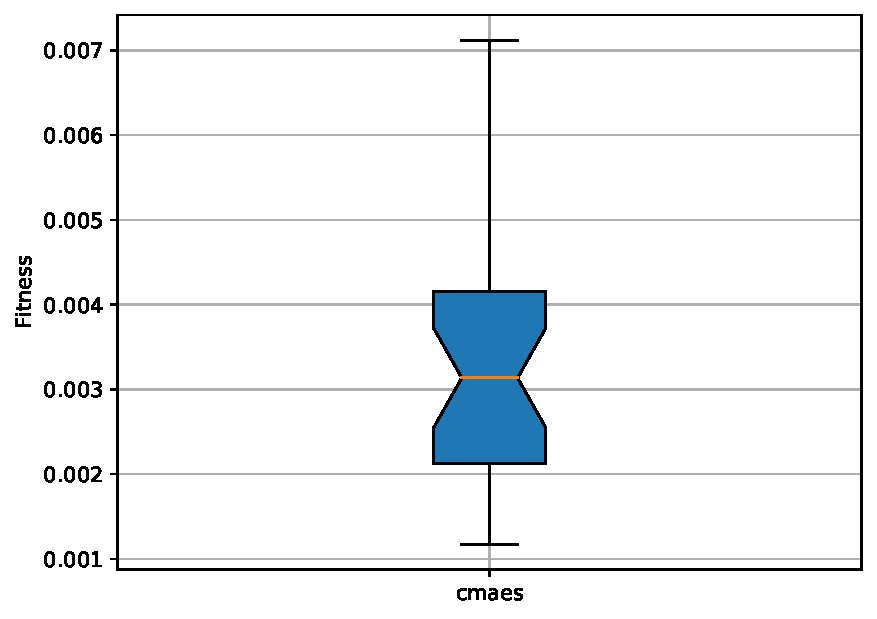
\includegraphics[width=75mm]{obrazky-figures/statistics/Benchmarks/Ackley/JOINED/cmaes_solutionsPlotsComparasion.pdf}
    \caption{Detail na výsledky algoritmu CMA-ES omezené optimalizace Ackleyho funkce.}
    \label{fg:bench:ackley:cmaes}
\end{figure}

\subsubsection*{Griwankova funkce}
\label{subsub:griewank:res}
Následující výsledky jsou agregací 30 běhu každého algoritmu. Parametry spuštění byly následující:
\begin{table}[H]
\centering
\resizebox{\textwidth}{!}{%
\begin{tabular}{|c|c|c|c|c|c|}
\hline
\multirow{3}{*}{\textbf{GA}} &
  \multirow{3}{*}{\begin{tabular}[c]{@{}c@{}}50 jedinců \\ v~populaci\end{tabular}} &
  \multirow{3}{*}{\begin{tabular}[c]{@{}c@{}}Turnajový \\ výběr\end{tabular}} &
  \multirow{3}{*}{\begin{tabular}[c]{@{}c@{}}Dvoubodové \\ křížení 80\%\end{tabular}} &
  \multirow{3}{*}{\begin{tabular}[c]{@{}c@{}}Mutace \\ 20\%\end{tabular}} &
  \multirow{3}{*}{\begin{tabular}[c]{@{}c@{}}Přežití nejlepších \\ bez ohledu \\ na generaci\end{tabular}} \\
 &
   &
   &
   &
   &
   \\
 &
   &
   &
   &
   &
   \\ \hline
\multirow{2}{*}{\textbf{SA}} &
  \multirow{2}{*}{\begin{tabular}[c]{@{}c@{}}Počáteční \\ teplota 2000\end{tabular}} &
  \multirow{2}{*}{Krok 1\%} &
  \multicolumn{3}{c|}{\multirow{2}{*}{Lineární chladící rozvrh}} \\
 &
   &
   &
  \multicolumn{3}{c|}{} \\ \hline
\textbf{Tabu} &
  \begin{tabular}[c]{@{}c@{}}20 prvků \\ v~tabu seznamu\end{tabular} &
  \multicolumn{4}{c|}{5 kandidátních řešení} \\ \hline
\textbf{DE} &
  \begin{tabular}[c]{@{}c@{}}40 jedinců \\ v~populaci\end{tabular} &
  \begin{tabular}[c]{@{}c@{}}Strategie \\ RAND-TO-BEST/1/BIN\end{tabular} &
  \begin{tabular}[c]{@{}c@{}}Šance rekombinace \\ 75\%\end{tabular} &
  \multicolumn{2}{c|}{\begin{tabular}[c]{@{}c@{}}Faktor zesílení \\ 0.5\end{tabular}} \\ \hline
\textbf{PSO} &
  75 částic &
  \multicolumn{2}{c|}{\begin{tabular}[c]{@{}c@{}}Akcelerační koeficienty \\ c1 = c2 = 2\end{tabular}} &
  \multicolumn{2}{c|}{\begin{tabular}[c]{@{}c@{}}Koeficient \\ setrvačnosti 0.5\end{tabular}} \\ \hline
\textbf{\begin{tabular}[c]{@{}c@{}}CMA\\   ES\end{tabular}} &
  \multicolumn{5}{c|}{\textit{Nevyžaduje vstupní parametry.}} \\ \hline
\end{tabular}%
}
\label{tb:bench:griewank}
\caption{Řídící parametry jednotlivých optimalizačních metod pro omezenou optimalizaci Griewankovi funkce.}
\end{table}
Výsledky je možné vidět na grafech~\ref{fg:bench:griewank:joined}. Funkce testuje globálnost metod a bylo tedy třeba podpořit tuto vlastnost vhodnými řídícími parametry algoritmů. Bohužel, i zde se omezení na $2000$ vyhodnocení ukázalo těžké. Diferenciální evoluce ani optimalizace rojem částic nestihli dokončit evoluci. Genetický algoritmus zdegeneroval, pravděpodobně nedostatečnou diverzitou způsobenou malou populací.

\begin{figure}[H]
\makebox[\textwidth][c]{
    \begin{tabular}{cc}
	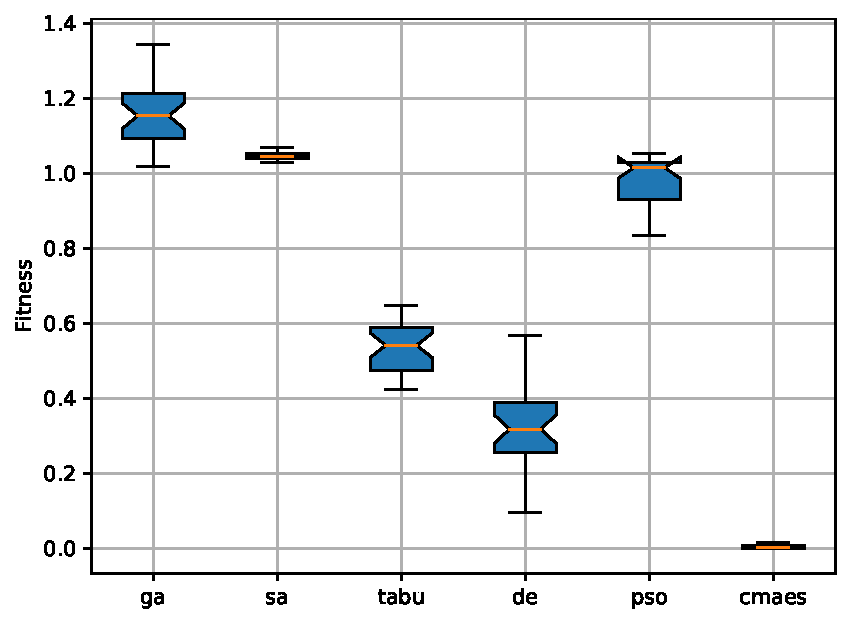
\includegraphics[width=75mm]{obrazky-figures/statistics/Benchmarks/Griewank/JOINED/solutionsPlotsComparasion.pdf}
    &
	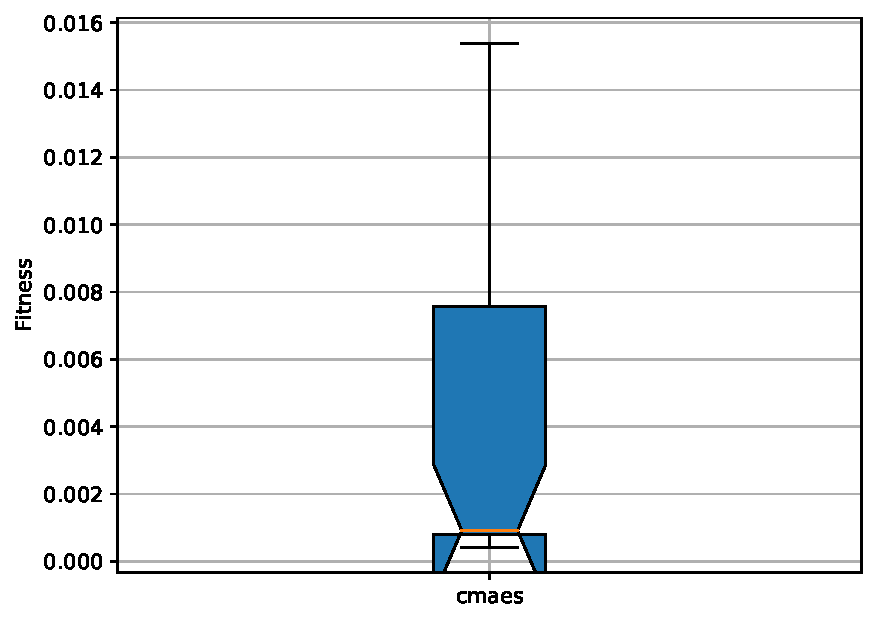
\includegraphics[width=75mm]{obrazky-figures/statistics/Benchmarks/Griewank/JOINED/cmaes_solutionsPlotsComparasion.pdf}
    \end{tabular}
    }
    \caption{Výsledky omezené optimalizace Griewankovi funkce. Vlevo výsledky všech algoritmů, vpravo detail na CMA-ES.}
    \label{fg:bench:griewank:joined}
\end{figure}
\subsubsection*{Rosenbrockova funkce}
\label{subsub:rosenbrock:res}
Následující výsledky jsou agregací 30 běhu každého algoritmu. Parametry spuštění byly následující:

\begin{table}[H]
\centering
\resizebox{\textwidth}{!}{%
\begin{tabular}{|c|c|c|c|c|c|}
\hline
\multirow{3}{*}{\textbf{GA}} &
  \multirow{3}{*}{\begin{tabular}[c]{@{}c@{}}64 jedinců \\ v~populaci\end{tabular}} &
  \multirow{3}{*}{\begin{tabular}[c]{@{}c@{}}Turnajový \\ výběr\end{tabular}} &
  \multirow{3}{*}{\begin{tabular}[c]{@{}c@{}}Dvoubodové \\ křížení 80\%\end{tabular}} &
  \multirow{3}{*}{\begin{tabular}[c]{@{}c@{}}Mutace \\ 5\%\end{tabular}} &
  \multirow{3}{*}{\begin{tabular}[c]{@{}c@{}}Přežití nejlepších \\ bez ohledu \\ na generaci\end{tabular}} \\
 &
   &
   &
   &
   &
   \\
 &
   &
   &
   &
   &
   \\ \hline
\multirow{2}{*}{\textbf{SA}} &
  \multirow{2}{*}{\begin{tabular}[c]{@{}c@{}}Počáteční \\ teplota 2000\end{tabular}} &
  \multirow{2}{*}{Krok 1\%} &
  \multicolumn{3}{c|}{\multirow{2}{*}{Lineární chladící rozvrh}} \\
 &
   &
   &
  \multicolumn{3}{c|}{} \\ \hline
\textbf{Tabu} &
  \begin{tabular}[c]{@{}c@{}}20 prvků \\ v~tabu seznamu\end{tabular} &
  \multicolumn{4}{c|}{5 kandidátních řešení} \\ \hline
\textbf{DE} &
  \begin{tabular}[c]{@{}c@{}}30 jedinců \\ v~populaci\end{tabular} &
  \begin{tabular}[c]{@{}c@{}}Strategie \\ BEST/1/BIN\end{tabular} &
  \begin{tabular}[c]{@{}c@{}}Šance rekombinace \\ 80\%\end{tabular} &
  \multicolumn{2}{c|}{\begin{tabular}[c]{@{}c@{}}Faktor zesílení \\ 0.5 až 0.7\end{tabular}} \\ \hline
\textbf{PSO} &
  75 částic &
  \multicolumn{2}{c|}{\begin{tabular}[c]{@{}c@{}}Akcelerační koeficienty \\ c1 = c2 = 2\end{tabular}} &
  \multicolumn{2}{c|}{\begin{tabular}[c]{@{}c@{}}Koeficient \\ setrvačnosti 0.5\end{tabular}} \\ \hline
\textbf{\begin{tabular}[c]{@{}c@{}}CMA\\   ES\end{tabular}} &
  \multicolumn{5}{c|}{\textit{Nevyžaduje vstupní parametry.}} \\ \hline
\end{tabular}%
}
\end{table}
Výsledky je možné vidět na grafech~\ref{fg:bench:rosen:joined},~\ref{fg:bench:rosen:joined} a~\ref{fg:bench:rosen:detail}. Optimum rosenbrockovi funkce leží v~hlubokém údolí, kde každý krok směrem k~optimu výrazně vylepšuje fitness. Na tomto testu ukázali svou sílu algoritmy využívající informace o~trasách či směru - diferenciální evoluce, pso a cma-es. Na druhou stranu je z~výsledků na první pohled patrné, že genetický algoritmus neuspěl. I~zde se ukázala jako problém diverzita (grafy~\ref{fg:bench:rosenbrock:ga:lastGen}, přestože jiným způsobem, než v~předchozích případech. Algoritmus neuvázl v~lokálním extrému; nedokázal dostatečně konvergovat, protože populace neobsahovala lepší jedince. Tabu prohledávání i simulované žíhání také nebyly schopný cíle dosáhnout, pravděpodobně z~důvodů špatně nastavené délky kroku. Optimalizace rojem částic a diferenciální evoluce opět nedokázali dokončit evoluci - v~momentě ukončení optimalizace stále vylepšovali svá řešení (patrné z~grafů~\ref{fg:bench:rosenbrock:pso:evoProg} a~\ref{fg:bench:rosenbrock:de:evoProg}).


Bohužel, i zde se omezení na $2000$ vyhodnocení ukázalo těžké. Diferenciální evoluce ani optimalizace rojem částic nestihli dokončit evoluci. Genetický algoritmus zdegeneroval, pravděpodobně nedostatečnou diverzitou způsobenou malou populací. Větší populace vyžadují více vyhodnocení a tím zase méně generací k~vylepšení řešení. Z~tohoto důvodu byla i nastavena nezvykle vysoká pravděpodobnost mutace; jako snaha o~podporu diverzity.

\begin{figure}[H]
\makebox[\textwidth][c]{
    \begin{tabular}{cc}
	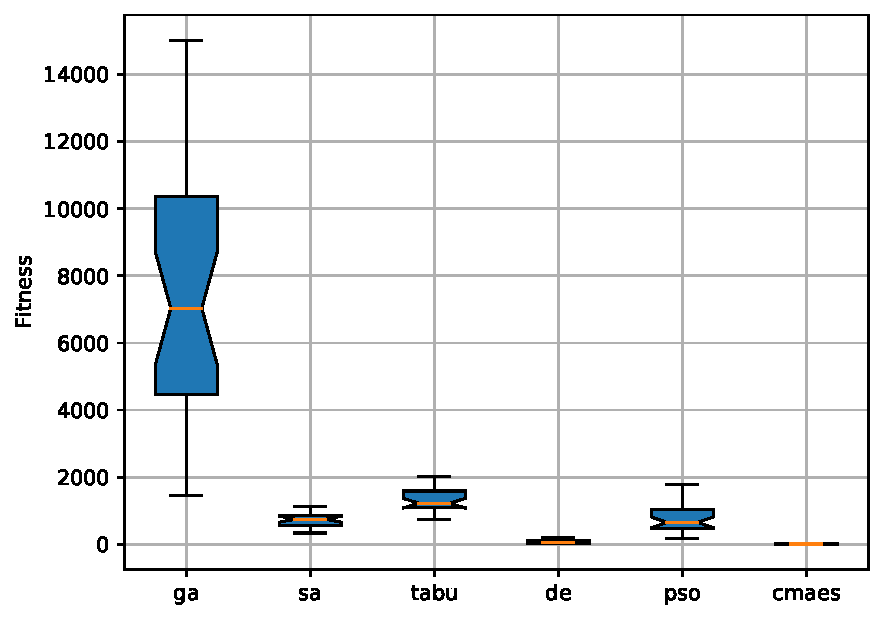
\includegraphics[width=75mm]{obrazky-figures/statistics/Benchmarks/Rosenbrock/JOINED/solutionsPlotsComparasion.pdf}
    &
	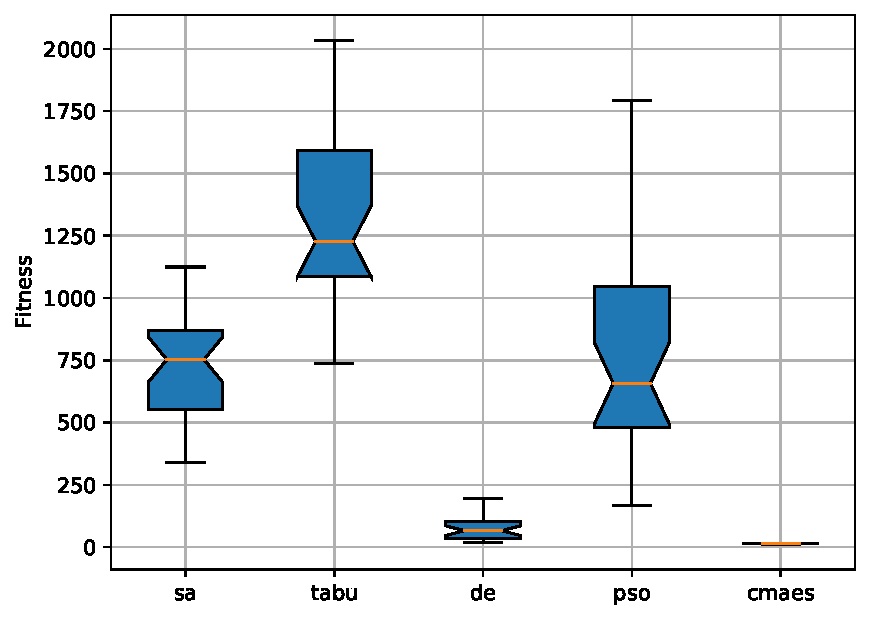
\includegraphics[width=75mm]{obrazky-figures/statistics/Benchmarks/Rosenbrock/JOINED/nonga_solutionsPlotsComparasion.pdf}
    \end{tabular}
    }
    \caption{Výsledky omezené optimalizace Rosenbrockovi funkce. Vlevo všechny algoritmy, vpravo vynechán genetický algoritmus.}
    \label{fg:bench:rosen:joined}
\end{figure}
\begin{figure}[H]
\makebox[\textwidth][c]{
    \begin{tabular}{cc}
	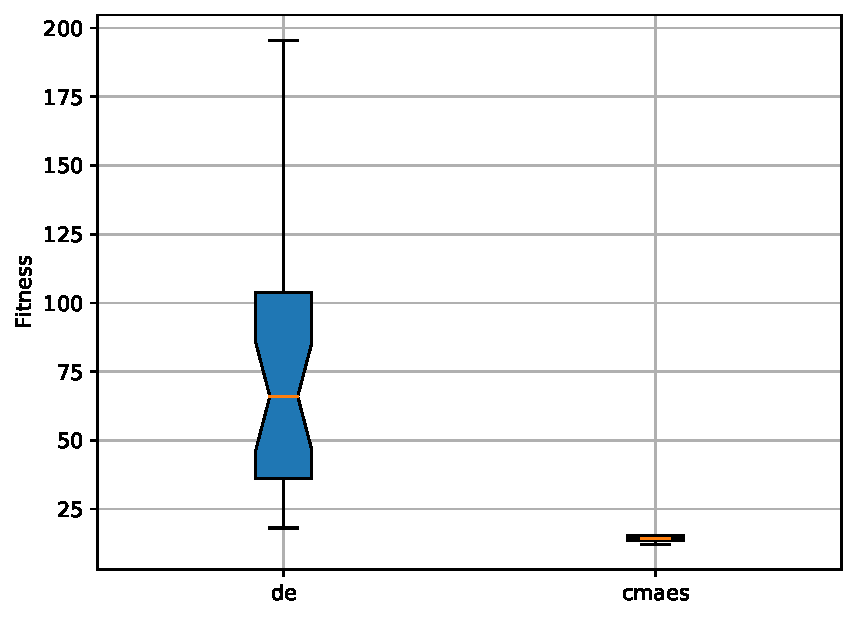
\includegraphics[width=75mm]{obrazky-figures/statistics/Benchmarks/Rosenbrock/JOINED/detail_solutionsPlotsComparasion.pdf}
    &
	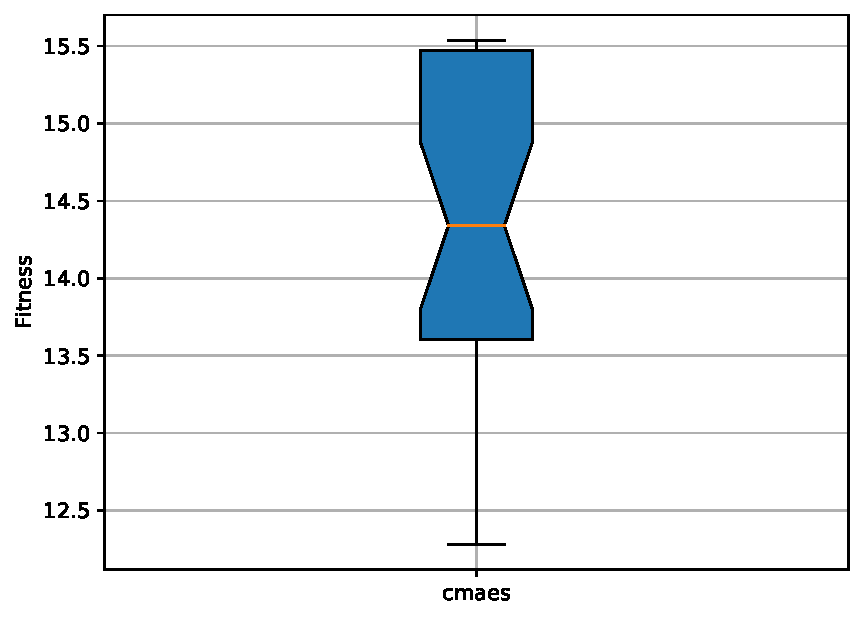
\includegraphics[width=75mm]{obrazky-figures/statistics/Benchmarks/Rosenbrock/JOINED/cmaes_solutionsPlotsComparasion.pdf}
    \end{tabular}
    }
    \caption{Výsledky omezené optimalizace Rosenbrockovi funkce. Vlevo detail na diferenciální evoluci a CMA-ES, vpravo CMA-ES samotná.}
    \label{fg:bench:rosen:detail}
\end{figure}

\subsection{Zhodnocení}
Testovací sada funkcí nebyla vybrána náhodně, každá vystavuje optimalizační metody jiným úskalím. Od konce: 
\begin{itemize}
    \item \textbf{Rosenbrockova funkce} testuje exploitační schopnosti metod - jak dobře dokáží konvergovat k~optimu.
    \item \textbf{Griewankova funkce} testovala explorační schopnost algoritmu. Funkce připomíná šum a algoritmus musel překonat množství lokálních optim, než se dostane ke globálnímu.
    \item \textbf{Ackleyho funkce} - první testovaná funkce měla za úkol otestovat obecnou schopnost optimalizačních metod. K~její optimalizaci je zapotřebí obou vlastností, exploraci i exploitace.
\end{itemize}
Cílem ovšem nebylo najít nejlepší obecný optimalizační algoritmus ale takovou evoluční metodu, která má největší potenciál řešit úlohu představenou v~kapitole~\ref{about} - plánování HIFU trajektorie. Platí tzv. \uv{No free lunch} teorém. 

\subsubsection{No free lunch teorém}
Teorém definovaný matematikem \textit{David H. Wolpert}. Všechny algoritmy, které hledají extrém účelové funkce, mají stejnou obecnou výkonost - pokud bychom zprůměrovaly jejich výsledky pro všechny možné účelové funkce, nenašli bychom rozdíl. Pokud je jeden algoritmus výkonnější nad množinou funkcí $A$, jiný bude výkonnější nad množinou funkcí $B$, která má stejnou kardinalitu.

\subsubsection{Závěry}
Z~výsledků~\ref{subsub:ackley:res},~\ref{subsub:griewank:res} a~\ref{subsub:rosenbrock:res} je patrné, že zavedená omezení a zvýšení dimenze problému jsou těžce překonatelné nástrahy. Genetický algoritmus trpí na problémy s~diverzitou populace, diferenciální evoluce a optimalizace rojem částic nedokáží dostatečně rychle konvergovat. Simulované žíhání i tabu prohledávání naopak nepoužívají populace řešení, nýbrž stále vylepšují své jedno nalezené. To jim dává jistou výhodu při omezeném množství vyhodnocení účelové funkce, ovšem i přes to nejsou díky povaze generování následujících stavů schopny konvergovat k~úzkému středu a nebo překonat lokální extrém v~pozdějších fázích optimalizace. Jako nejlepší algoritmus při řešení všech optimalizačních testů se ukázala metoda CMA-ES, jejíž flexibilní generování kandidátních řešení na základě předchozí evoluční cesty umožňuje dobrou konvergenci i škálovatelnost s~velikostí dimenze.



\subsubsection{Transformace problému}
Vhodný algoritmus pro řešení testovací množiny ovšem ještě nezaručuje jeho schopnost řešit i problém hledání trajektorie sonikací, stále platí \uv{No free lunch} teorém. Kvůli této skutečnosti je třeba zjistit, jestli se tento problém alespoň částečně nepodobá nějakému z~testovací sady.

Jak bylo popsáno v~kapitole~\ref{about}, systém HIFU je heterogenní systém, ve kterém se vyskytuje šum. Také bylo zmíněno, že cévy v~blízkosti cíleného místa odvádějí energii. Není příliš těžké si představit transformaci tohoto problému - pokud budeme tyto cévy považovat za lokální minima a šum a ne-homogennost za jisté \uv{spády} na povrchu takovéto funkce. Dále je přitěžující skutečnost, že hledané proměnné jsou na sobě závislé, a díky povaze kódování a průběhu simulace - sonikace jsou prováděny sekvenčně za sebou a pořadí těchto sonikací je důležité jen do jisté míry - lze prohlásit, že každé řešení problému má i svou variantu, která se liší pouze pořadím provedení. Sonikace jsou na sobě také velice závislé, malá změna v~parametrech jedné sonikace může mít za následek velké skoky v~hodnotách fitness - sonikace pokrývají kruhovou oblast, kterou je jednoduché přesáhnout okraje nebo například způsobit, že jiná sonikace, která doposud vylepšovala fitness, je najednou zbytečná. To vše má za následek obtížnou konvergenci k~optimu. V~poslední řadě jsou kraje stavového prostoru penalizovány (přesah na zdravou tkáň je nežádoucí). Tento popis není příliš podobný žádné z~funkcí. Testuje schopnost prohledávat i konvergovat ke skutečně optimální kombinaci. Těžká konvergence odpovídá nejlépe funkci \textbf{Rosenbrock}, zatímco případné lokální extrémy a strmý spád funkci odpovídá testu \textbf{Ackley}. 

%%%%%%%%%%%%%%%%%%%%%%%%%%%%%%%%%%%%%%%%%%%%%%%%%%%
%%%%%%%%%%%%%%%%%%%%%%%%%%%%%%%%%%%%%%%%%%%%%%%%%%%
\chapter{Model šíření tepla ve tkáních}
\label{chap:5}
Tato kapitola naváže na popis z~kapitoly~\ref{about} a více představí implementovaný model. Zdrojový článek~\cite{FITPUB11696} pracoval s~implementací v~prostředí MATLAB, která byla později přepsána do formy \emph{mex} funkce pro urychlení výpočtu za pomoci paralelizačních technik - \emph{multi-threadingu} a vektorizace za pomoci \emph{OMP}. Toto řešení bylo pro potřeby mé práce dále upraveno takto:
\begin{itemize}
    \item Definovaná funkce byla základem pro výpočetní model v~jádru účelové funkce. Pro potřeby této práce byl model zbaven \emph{mex} a tím i \emph{MATLAB} rozhraní, a upraven pro použití v~jazyce C++. 
    \item Přidáno načítání dat média ze souborů. Jedná se o~jednoduché čtení matice čísel z~několika souborů, kde každý soubor reprezentuje jinou relevantní informaci o~médii, jako například hustotu či tepelnou vodivost. 
    \item Implementováno podpůrné jádro pro práci s~maticemi, které slouží pro definice cílové a penalizační mapy. Za tímto účelem vzniklo několik výpočetních funkcí a obal, jehož vstupem jsou soubory \texttt{prohibitedMapCircles.dat} a \texttt{targetMapCircles.dat}, které definují své mapy ve formě libovolného množství geometrických kruhů. Tyto kruhy jsou popsány čtveřicí $(X,Y,R,V)$, kde $X$ a $Y$ jsou souřadnice středu, $R$ je poloměrem a $V$ je hodnotou váhy. Hodnoty jsou odděleny čárkou a jednotlivé kruhy odděleny novým řádkem. Váha kruhu reprezentuje hodnotu penalizace či závažnost cíle. Modul postupně tyto kruhy vykreslí do mřížky o~velikosti média a vyplní právě zadanou hodnotou. V~případě, že se kruhy překryjí, se hodnoty na těchto místech: \begin{itemize}
        \item při definici penalizační mapy sečtou
        \item při definici cíle je nad těmito hodnotami provedena funkce $max(...)$
    \end{itemize}
    Tím je možné vytvořit penalizační i cílenou mapu nad libovolným médiem.  
    Pro takto vytvořené mapy vznikly funkce umožňující jejich sečtení, produkt, či práhování hodnot aplikací filtru.
    \item Z~\emph{MATLAB} implementace přepsáno generování matice přidané tepelné energie. Tato matice reprezentuje jednu sonikaci a její tvar je aproximací za pomoci Gaussova rozložení ve $2D$ prostoru. Takto definované sonikace jsou následně vstupem samotné simulace.
    \item V~poslední řadě byla proveden analýza výpočetního výkonu samotné simulace za pomoci nástrojů \emph{Intel VTune™ Profiler}. Na základě těchto výsledků byly přepracovány již existující paralelizační techniky na modernější a čitelnější variantu direktiv \emph{OMP} pro překladač \emph{Intel Compiler 2019a}.
\end{itemize}


Tyto části, spolu se vstupním bodem splňujícím rozhraní \texttt{FitnessFunction.h} z~kapitoly~\ref{impl}, vytváří optimalizovanou účelovou funkci.


\section{Data}
Pro spuštění simulace sonikací jsou potřeba dva druhy dat. Za prvé data definující médium, ve kterém se teplo šíří, a za druhé segmentová mapa $D$, která každému bodu média přiřazuje hodnotu. Ta je po dokončení simulace použita pro výpočet fitness.

\subsection{Médium}
Médium, se kterým model pracuje, je reprezentováno jako soustava několika matic $X \times Y$ a hodnoty $dx$, která ukazuje skutečnou vzdálenost (v~$mm$) mezi jednotlivými body matice:
\begin{itemize}
    \item matice teploty $T$ - momentální teplota v~\degree C v~jednotlivých bodech média.
    \item matice hustoty $\rho$ - fyzikální hustota látek v~médiu (v~$kg*m^{-3}$ ).
    \item matice měrné tepelné kapacity $C$ - množství tepelné energie potřebné k~ohřátí 1$kg$ látky o~jeden teplotní stupeň ($J *kg^{-1}*K^{-1}$).
\end{itemize}
Jako médium byl využit open-source voxelový model \emph{Austin Woman}~\cite{austinwoman}. Jedná se o~dataset pořízený jako součást projektu \emph{Visible Human} ze \emph{U.S. National Library of Mediciny}. 
Model pracuje s~reprezentací tohoto média v~prostoru $495 \times 495$ a $dx = 0.2e-3$. Tyto data jsou umístěna ve vlastních souborech pro případnou snadnou úpravu či náhradu za jiný dataset.

\subsection{Omezení}
Jak již bylo zmíněno v~předchozí kapitole, z~důvodu výpočetní náročnosti bylo omezeno maximální počet vyhodnocení kompletní simulace na $2000$\footnote{Hodnota nebyla kontrolována před každým provedením simulace, nýbrž na začátku generací. Následkem je, že populační metody mohou tuto hodnotu přesáhnout pro dokončení generace} na jeden běh optimalizační metody. Kompletní simulací je myšleno provedení všech $n$ sonikací obsažených v~chromozomu (tedy dohromady $2000 * n$ výpočtů šíření tepla). Zároveň jsou pro každý z~vybraných problémů definována globální omezení tohoto typu:
\begin{itemize}
    \item Stavový prostor pro souřadnice sonikace byl omezen na hodnoty $x_l < x(i) < x_h$ a $y_l < y(i) < y_h$.
    \item Stavový prostor proměnných určujících dobu záření a chlazení byl omezen následovně : $0 < t_{on}$ a $0 < t_{off}$.
    \item Stavový prostor každé proměnné byl spojen do tvaru toroidu - překročením hranice se metoda dostává na druhou stranu.
    \item Optimalizace je prohlášena za dokončenou v~případě, kdy $f(I) < 10$ (fitness na začátku optimalizce se pohybuje v~řádech $10^3 - 10^4$ a vzhledem k~rasterizaci problému, nepřesnosti čísel s~plovoucí desetinou čárkou a použitým aproximacím, lze takto nízkou fitness považovat za optimum), nebo dosažením zmíněné hodnoty $2000$ fitness vyhodnocení.
\end{itemize}
 
\section{Průběh simulace}
V~momentě, kdy jsou k~dispozici data popisující médium, segmentová mapa i vektor sonikací, může začít simulace. Pro každou sonikaci se vytvoří matice přidaného tepla $Q$. Tato matice (opět $X \times Y$) je vygenerována za pomoci dvourozměrného normálního rozložení se středem v~bodě matice $Q_{x(i)y(i)}$\footnote{Tato distribuce je aproximací skutečnosti, jelikož modely schopny precizní simulace jsou výpočetně náročné a přidávat je do již dost výpočetně náročné simulace šíření by způsobilo rapidní zpomalení výpočtu}. Takto vytvořené matice se sekvenčně aplikují na model média tak, že pro každou sonikaci je spuštěna simulace šíření tepla v~médii a spočteno kumulované teplo - prostorová termální mapa $CEM{43}$. Na základě této mapy je poté provedeno práhování, které označí všechny body média, které byly zničeny termální ablací. Práhování, resp. výsledná maska, je popsána vztahem~\ref{eq:cemMat}. Rovnice převzaty ze~\cite{FITPUB11696}.
\begin{equation}
    C_{ij} = \begin{cases} 
            0       & \text{pokud } CEM43_{ij} \le 240\\
            1       & \text{jinak}
        \end{cases}\\
        \label{eq:cemMat}
\end{equation}{}

Fitness funkce je poté vypočtena vztahem~\ref{eq:hifuFitness}:
\begin{equation}
    f = \int_{0}^{X}\int_{0}^{Y}(D * \overline{C}) + (D * C)) dxdy
    \label{eq:hifuFitness}
\end{equation}

\section{Testované útvary}
V~následující sekci jsou popsány dva vybrané útvary pro pokus o~optimalizaci trajektorie. Útvary představují dva typické modely cílené tkáně při praktickém použití. Tyto útvary byly pojmenovány jako \uv{skvrna} a \uv{květina}, podle tvarů, které připomínají autorovi. Obě tyto mapy byly vytvořeny na médiu z~\emph{AustinWoman}.

\subsection{Skrvna}
Cíl, označený jako skvrna, je monolitická cílová oblast definována v~rozmezích $272 < x(i) < 342$ a $233 < y(i) < 293$. Spolu s~penalizační mapou je tento model zobrazen na obrázku~\ref{fg:hifu:usecase:blob}. Jedná se o~citelně jednodušší z~obou testů, především z~důvodu pozitivního efektu akumulovaného tepla ve tkáních. Ablace středu tohoto útvaru má prioritu před okraji. Útvar tohoto typu si není příliš těžké představit i v~reálném světě. 

\begin{figure}[H]
    \centering
	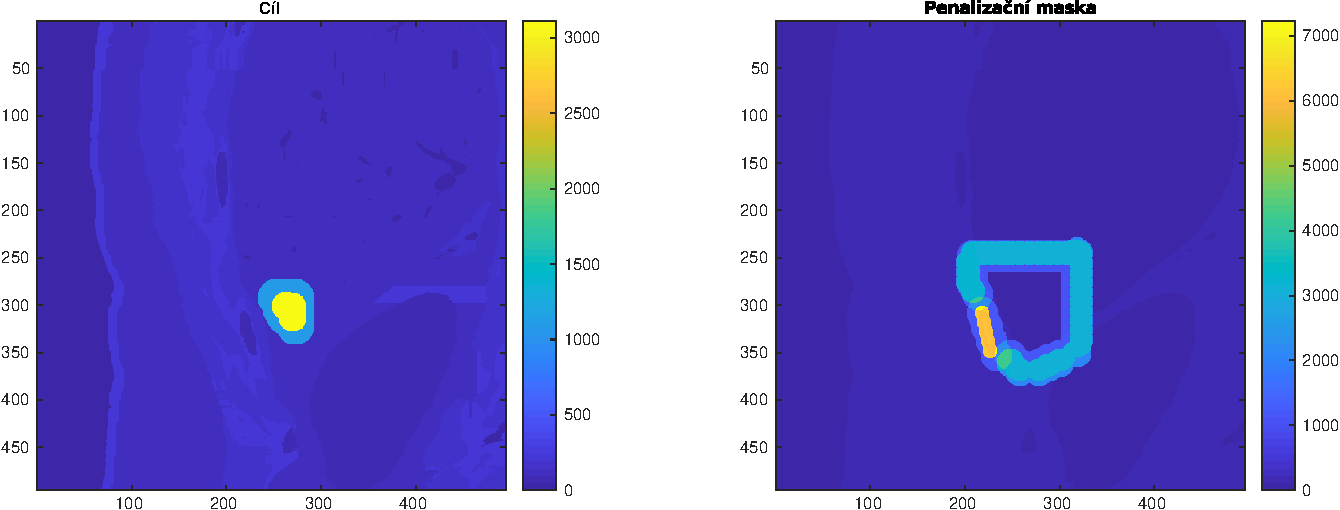
\includegraphics[width=0.8\textwidth]{obrazky-figures/hifuUseCase/blob_croped.pdf}
	\caption{Diskrétní barevná mapa útvaru skvrna pro testování optimalizace trajektorie HIFU sonikací. Vlevo mapa definující cíl, který je třeba vypálit. Vpravo mapa ukazující penalizovanou oblast, kterou je třeba uchránit.}
	\label{fg:hifu:usecase:blob}
\end{figure}

\subsection{Květina}
Cíl, označený jako květina, je pravidelný, symterický útvar, v~jehož středu se nachází zdravá tkáň, kterou je nutno ochránit. Celá cílová oblast je definována v~rozmezích $208 < x(i) < 288$ a $208 < y(i) < 288$. Spolu s~penalizační mapou je tento model zobrazen na obrázku~\ref{fg:hifu:usecase:flower}. Z~experimentů se ukazuje, že se jedná o~těžší z~modelů, především kvůli efektu akumulovaného tepla právě ve zdravém středu objektu. Prováděné sonikace se překrývají a v~okolí středu postupně akumulují teplo. Tím vzniká kladná zpětná vazba a vysoce se zvyšuje závislost na pořadí provedení řetězu sonikací. Tento jev existuje sice i v~případě problému typu skvrna, tam je ovšem pozitivním faktorem, jelikož je tvar ucelený a střed útvaru je cílem. V~reálném světě tento problém reprezentuje zhoubnou tkáň, obrostlou například okolo močové trubice.

\begin{figure}[H]
    \centering
	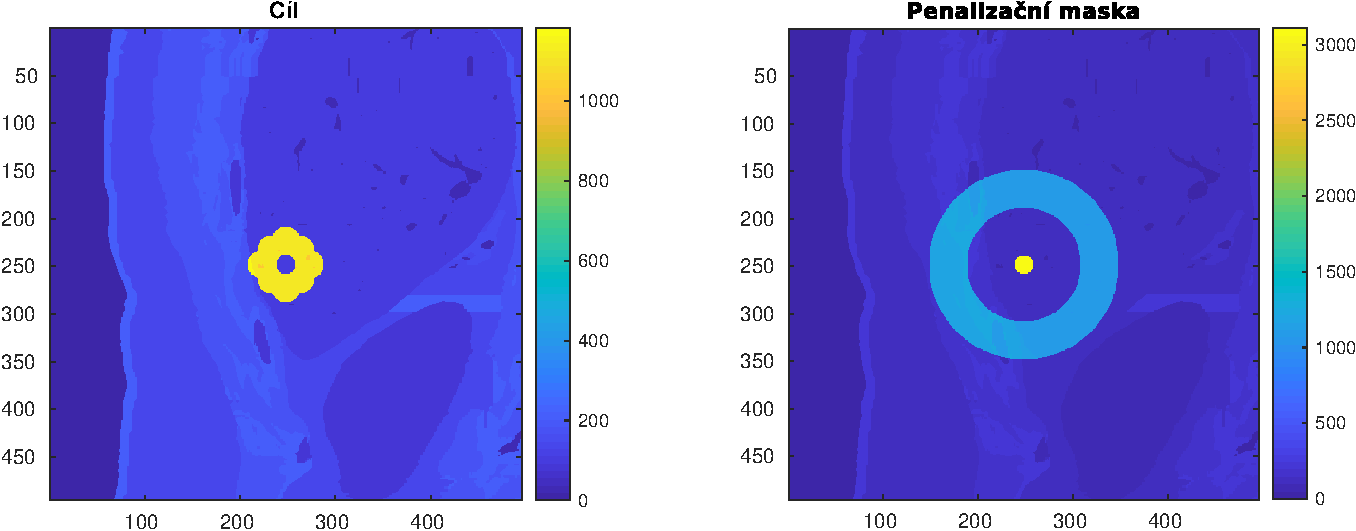
\includegraphics[width=0.8\textwidth]{obrazky-figures/hifuUseCase/flower_croped.pdf}
	\caption{Diskrétní barevná mapa útvaru květina pro testování optimalizace trajektorie HIFU sonikací. Vlevo mapa definující cíl, který je třeba vypálit. Vpravo mapa ukazující penalizovanou oblast, kterou je třeba uchránit.}
	\label{fg:hifu:usecase:flower}
\end{figure}
	
	

\section{Výsledky}
V~následující sekci jsou prezentovány agregované výsledky $15$ nezávislých běhů optimalizační metody. V~první části je ukázána schopnost algoritmů hledat optimum při malém počtu sonikací ($4$ sonikace). Tento test je prováděn na problému typu skvrna a není relevantní pro reálné případy, při kterých jsou použity desítky sonikací, nýbrž jako důkaz koncepce použití těchto metod.
Následně budou prezentovány výsledky na vyšších počtech sonikací. Skvrna bude vyžita znovu, tentokrát pro hledání trajektorie o~$20$ sonikacích. Dále pak bude ukázáno $15$ sonikací pro oblast typu květina. Tyto hodnoty byly vybrány empiricky s~ohledem na daný problém a časovou náročnost výpočtů.

Výpočty byly provedeny na superpočítači \emph{Salomon} v~rámci projektu \emph{IT4Innovations}. V~součtu, včetně experimentů s~parametry, bylo využito $\textbf{64956}$ \textbf{hodin} normovaného procesorového času. U~grafů prezentujících poslední generace, případně rozptyl běhu, lze pozorovat výřezy na stranách - tzv. \uv{notche}. Tento notch představuje interval spolehlivosti $95\%$ kolem mediánu. Pokud se notche dvou rozdílných generací \textit{nepřekrývají} (tedy spodní konec výřezu není níže, než svrchní konec jiného), lze s~$95\%$ důvěrou tvrdit, že se od sebe liší.

\subsection{Skvrna - malý počet sonikací}
Hledání optimální trajektorie pro HIFU operaci s~nízkým počtem sonikací bylo spuštěno s~následujícími parametry:
\begin{table}[H]
\centering
\resizebox{\textwidth}{!}{%
\begin{tabular}{|c|c|c|c|c|c|}
\hline
\multirow{3}{*}{\textbf{GA}} &
  \multirow{3}{*}{\begin{tabular}[c]{@{}c@{}}64 jedinců \\ v~populaci\end{tabular}} &
  \multirow{3}{*}{\begin{tabular}[c]{@{}c@{}}Turnajový \\ výběr\end{tabular}} &
  \multirow{3}{*}{\begin{tabular}[c]{@{}c@{}}Dvoubodové \\ křížení 80\%\end{tabular}} &
  \multirow{3}{*}{\begin{tabular}[c]{@{}c@{}}Mutace \\ 20\%\end{tabular}} &
  \multirow{3}{*}{\begin{tabular}[c]{@{}c@{}}Přežití nejlepších \\ bez ohledu \\ na generaci\end{tabular}} \\
 &
   &
   &
   &
   &
   \\
 &
   &
   &
   &
   &
   \\ \hline
\multirow{2}{*}{\textbf{SA}} &
  \multirow{2}{*}{\begin{tabular}[c]{@{}c@{}}Počáteční \\ teplota 2000\end{tabular}} &
  \multirow{2}{*}{Krok 1\%} &
  \multicolumn{3}{c|}{\multirow{2}{*}{Lineární chladící rozvrh}} \\
 &
   &
   &
  \multicolumn{3}{c|}{} \\ \hline
\textbf{Tabu} &
  \begin{tabular}[c]{@{}c@{}}20 prvků \\ v~tabu seznamu\end{tabular} &
  \multicolumn{4}{c|}{5 kandidátních řešení} \\ \hline
\textbf{DE} &
  \begin{tabular}[c]{@{}c@{}}25 jedinců \\ v~populaci\end{tabular} &
  \begin{tabular}[c]{@{}c@{}}Strategie \\ BEST/1/BIN\end{tabular} &
  \begin{tabular}[c]{@{}c@{}}Šance rekombinace \\ 90\%\end{tabular} &
  \multicolumn{2}{c|}{\begin{tabular}[c]{@{}c@{}}Faktor zesílení \\ 0.5 až 0.9\end{tabular}} \\ \hline
\textbf{PSO} &
  64 částic &
  \multicolumn{2}{c|}{\begin{tabular}[c]{@{}c@{}}Akcelerační koeficienty \\ c1 = c2 = 2\end{tabular}} &
  \multicolumn{2}{c|}{\begin{tabular}[c]{@{}c@{}}Koeficient \\ setrvačnosti 0.5\end{tabular}} \\ \hline
\textbf{\begin{tabular}[c]{@{}c@{}}CMA\\   ES\end{tabular}} &
  \multicolumn{5}{c|}{\textit{Nevyžaduje vstupní parametry.}} \\ \hline
\end{tabular}%
}
\caption{Tabulka řídících parametrů použitých při optimalizaci modelu skvrna malým počtem sonikací.}
\end{table}

\subsubsection{Genetický algoritmus}
Lze vidět, že genetický algoritmus nebyl příliš úspěšný při hledání optima. Populace většiny běhů degenerovala - graf~\ref{fg:hifu:ga:lastGen} - a ani přes nadmíru vysokou pravděpodobnost mutace se nepodařilo udržet diverzitu. Bohužel, jedním z~hlavních prvků pro udržení různorodosti v~GA je velikost populace v~kontextu dimenze problému. S~velikostí populace ovšem rychle roste počet kandidátních řešení a tím i počet evaluací. Zvětšením populace by mohla rozrůst diverzita, algoritmus by ale nemusel mít dostatečný počet evaluací ke konvergenci.
\begin{figure}[H]
\begin{minipage}[t]{0.475\linewidth}
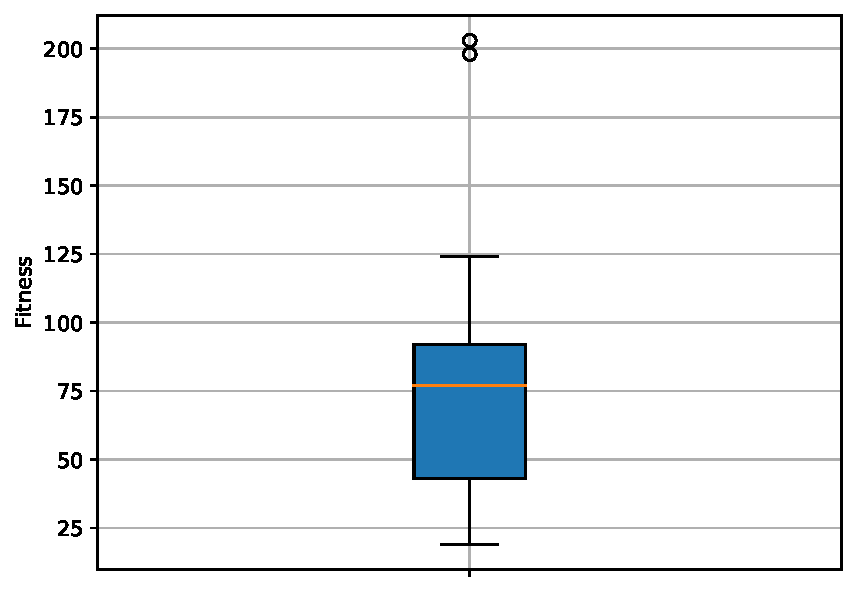
\includegraphics[width=\linewidth]{obrazky-figures/statistics/HIFU/blob/4/GA/bestsBoxplot_WithOutliers.pdf}
\caption{Boxplot nejlepších výsledků všech $15$ běhů GA.}
\label{fg:hifu:ga:best}
\end{minipage}
\hfill
\begin{minipage}[t]{0.475\linewidth}
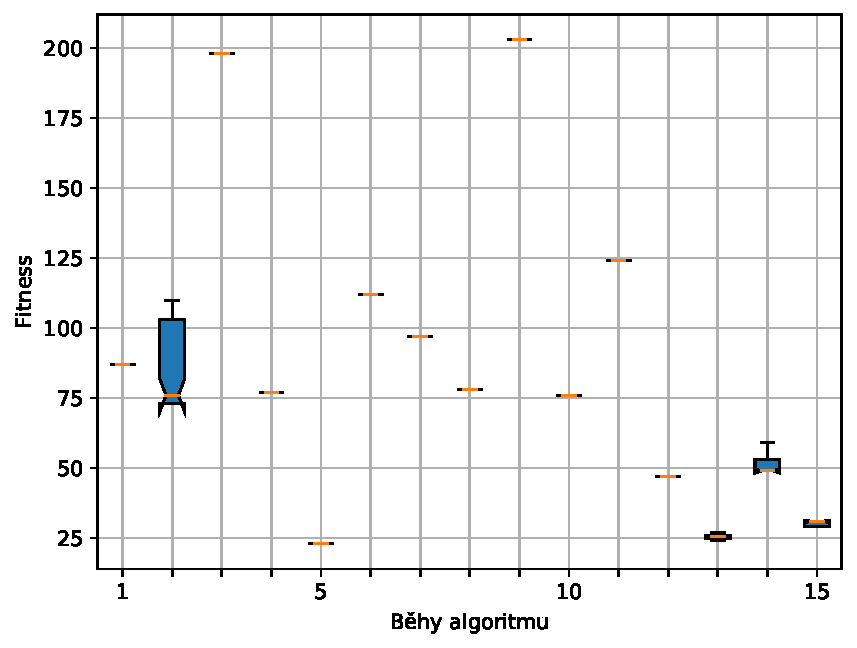
\includegraphics[width=\linewidth]{obrazky-figures/statistics/HIFU/blob/4/GA/lastGenBoxplots.pdf}
\caption{Boxplot stavu poslední generace všech $15$ běhů GA. Lze vidět, že docházelo k~degeneraci populace.}
\label{fg:hifu:ga:lastGen}
\end{minipage}
\end{figure}


\begin{figure}[H]
\begin{minipage}[t]{0.475\linewidth}
	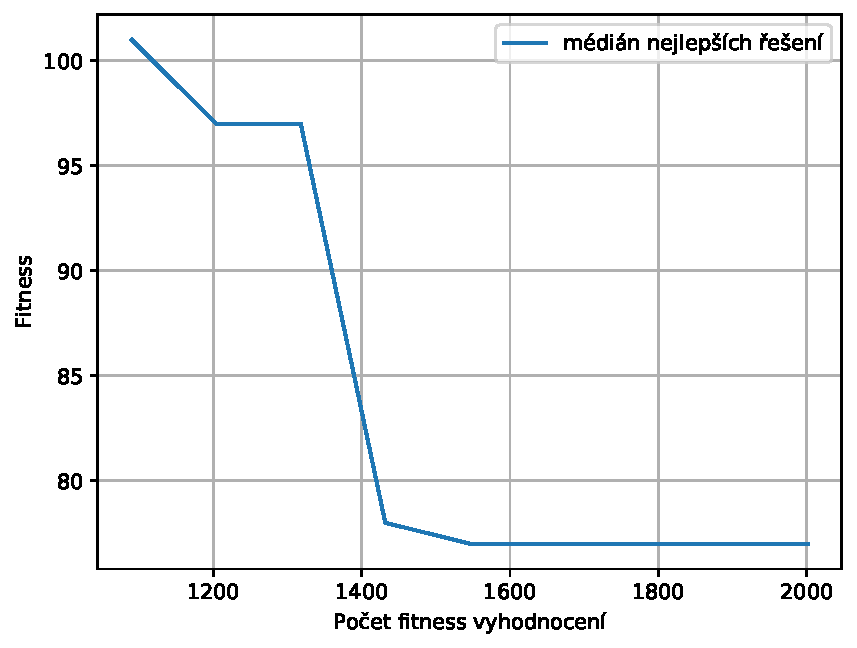
\includegraphics[width=\textwidth]{obrazky-figures/statistics/HIFU/blob/4/GA/bestsToFitness_1.pdf}
	\caption{Poměr mediánu nejlepších nalezených řešení vůči počtu evaluací fitness funkce. Zobrazena až druhá poloviny optimalizace.}
	\label{fg:hifu:ga:fitPerf}
\end{minipage}
\hfill
\begin{minipage}[t]{0.475\linewidth}
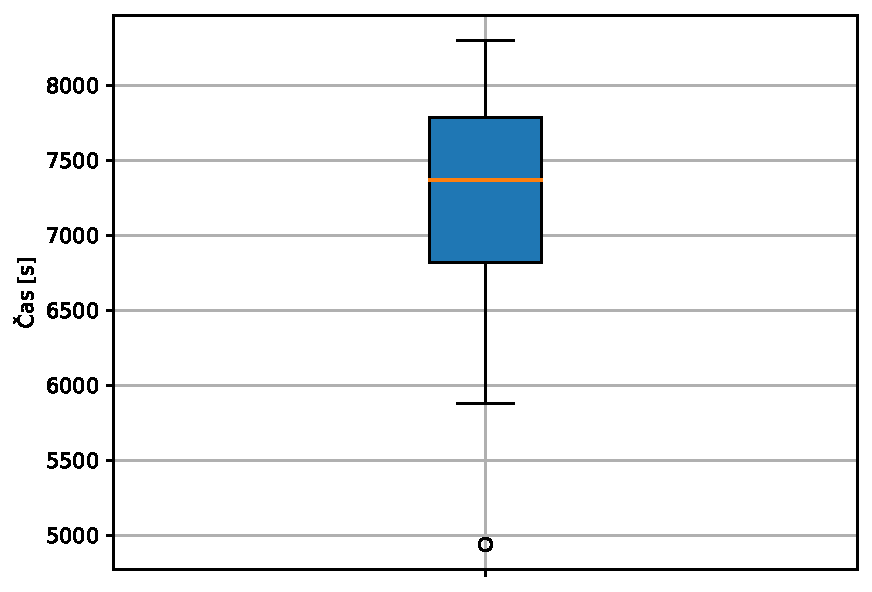
\includegraphics[width=\linewidth]{obrazky-figures/statistics/HIFU/blob/4/GA/timeBoxplot_WithOutliers.pdf}
\caption{Boxplot času potřebného k~dokončení optimalizace ve vteřinách. ($7200s = 2h$)}
\label{fg:hifu:ga:time}
\end{minipage}
\end{figure}

\begin{figure}[H]
    \makebox[\textwidth][c]{
    \begin{tabular}{cc}
	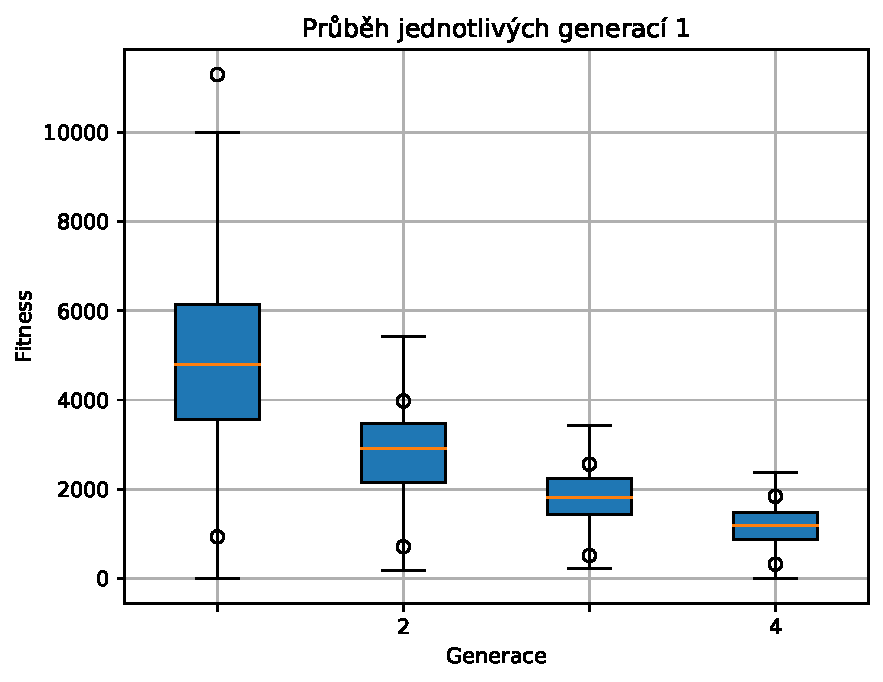
\includegraphics[width=75mm]{obrazky-figures/statistics/HIFU/blob/4/GA/evolutionProgress_0.pdf}
    &
	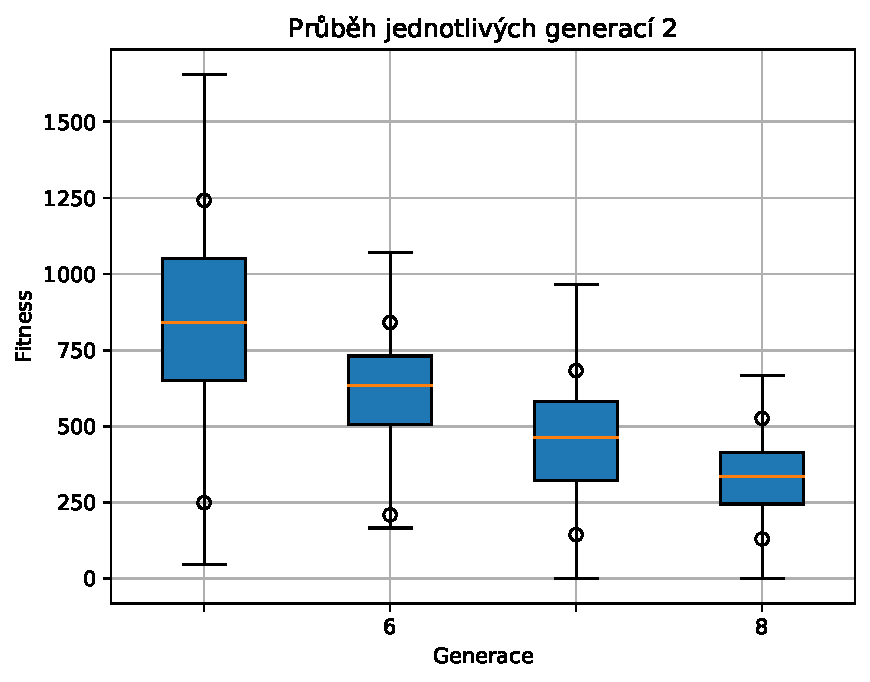
\includegraphics[width=75mm]{obrazky-figures/statistics/HIFU/blob/4/GA/evolutionProgress_1.pdf}
    &
	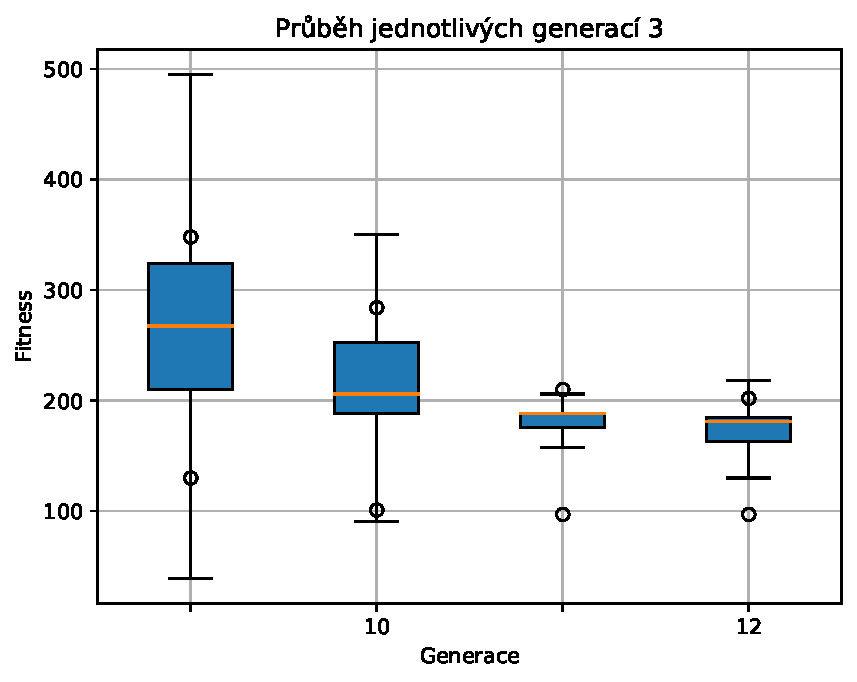
\includegraphics[width=75mm]{obrazky-figures/statistics/HIFU/blob/4/GA/evolutionProgress_2.pdf}
    &
	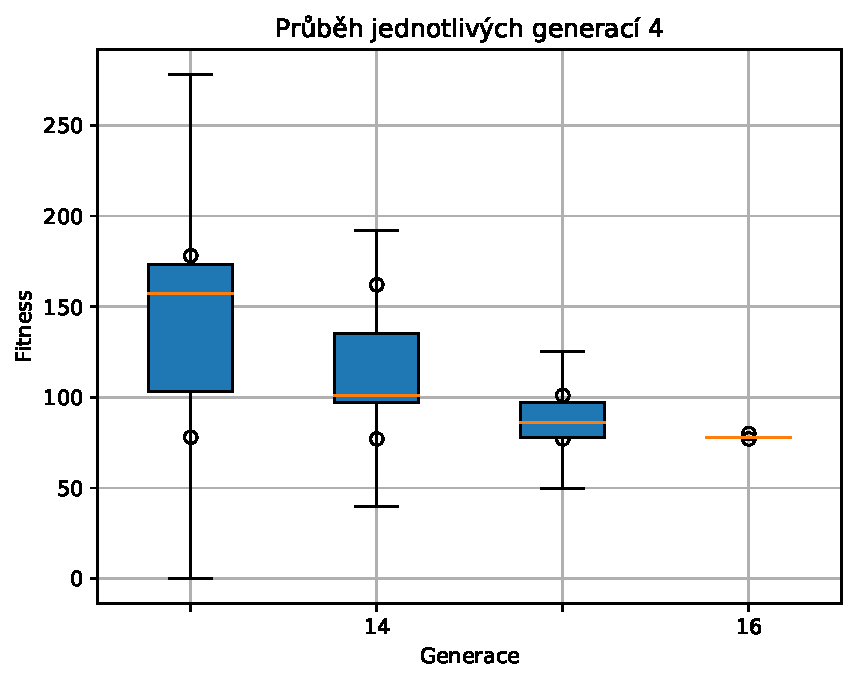
\includegraphics[width=75mm]{obrazky-figures/statistics/HIFU/blob/4/GA/evolutionProgress_3.pdf}
    \end{tabular}
    }
    \caption{Evoluční průběh GA. Data jsou mediány ze všech běhů v~konkrétních generacích. Graf rozdělen na čtvrtiny pro větší detail. Body ukazují medián nejlepších a nejhorších nalezených řešení v~dané generaci.}
    \label{fg:hifu:ga:evoProg}
\end{figure}



\subsubsection{Simulované žíhání}
Simulované žíhání bylo překvapivě úspěšné. Vzhledem k~tomu, že se nejedná o~populační algoritmus nebylo třeba řešit problémy s~diverzitou. Vyzdvihněme, že na mediánovou hodnotu $70$ se dostalo již za tisíc iterací~-~\ref{fg:hifu:sa:fitPerf}. V~případech, kdy by taková fitness byla dostatečná, by se SA dalo považovat za velice efektivní algoritmus pro optimalizaci problému hledání trajektorie.
\begin{figure}[H]
\begin{minipage}[t]{0.475\linewidth}
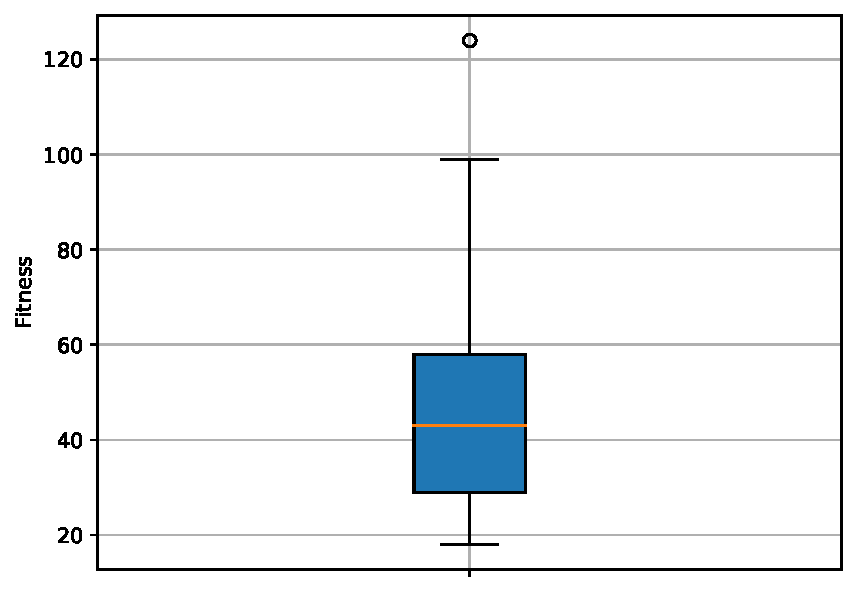
\includegraphics[width=\linewidth]{obrazky-figures/statistics/HIFU/blob/4/SA/bestsBoxplot_WithOutliers.pdf}
\caption{Boxplot nejlepších výsledků všech $15$ běhů SA.}
\label{fg:hifu:sa:best}
\end{minipage}
\hfill
\begin{minipage}[t]{0.475\linewidth}
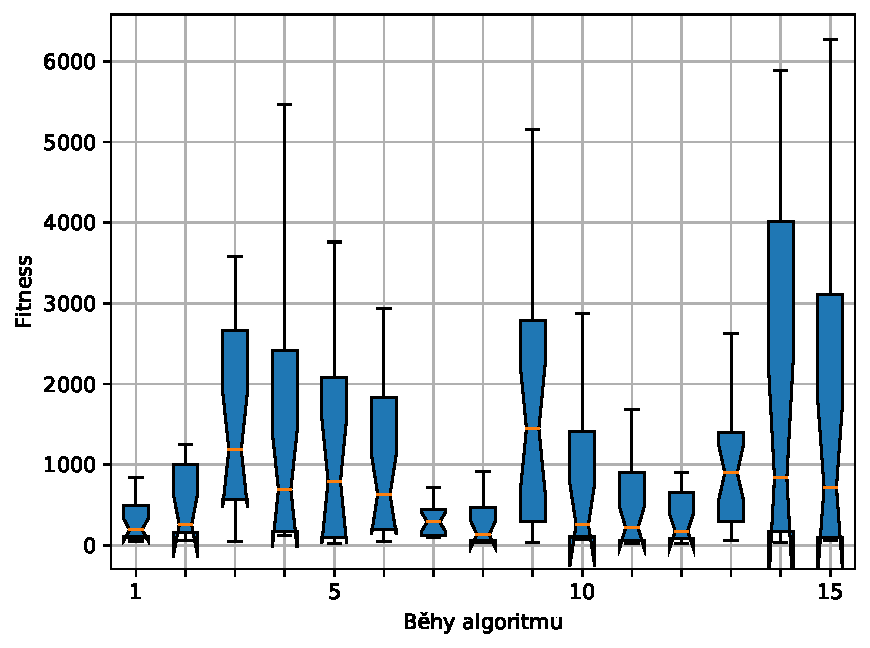
\includegraphics[width=\linewidth]{obrazky-figures/statistics/HIFU/blob/4/SA/lastGenBoxplots.pdf}
\caption{Boxplot ukazující rozptyl fitness, jaký každý běh SA prohledal.}
\label{fg:hifu:sa:lastGen}
\end{minipage}
\end{figure}

\begin{figure}[H]
\begin{minipage}[t]{0.475\linewidth}
	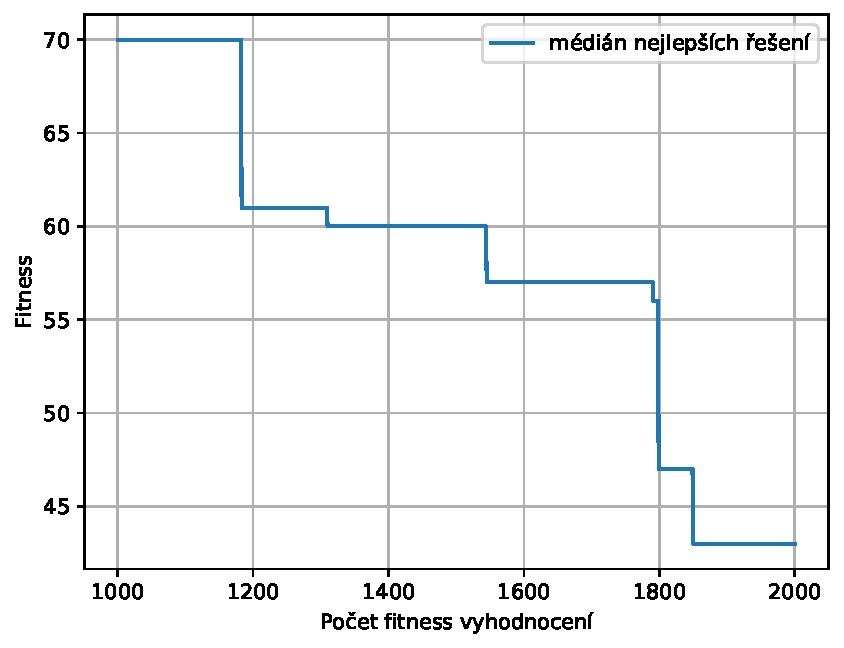
\includegraphics[width=\textwidth]{obrazky-figures/statistics/HIFU/blob/4/SA/bestsToFitness_1.pdf}
	\caption{Poměr médiánu nejlepších nalezených řešení vůči počtu evaluací fitness funkce.  Zobrazena až druhá poloviny optimalizace.}
	\label{fg:hifu:sa:fitPerf}
\end{minipage}
\hfill
\begin{minipage}[t]{0.475\linewidth}
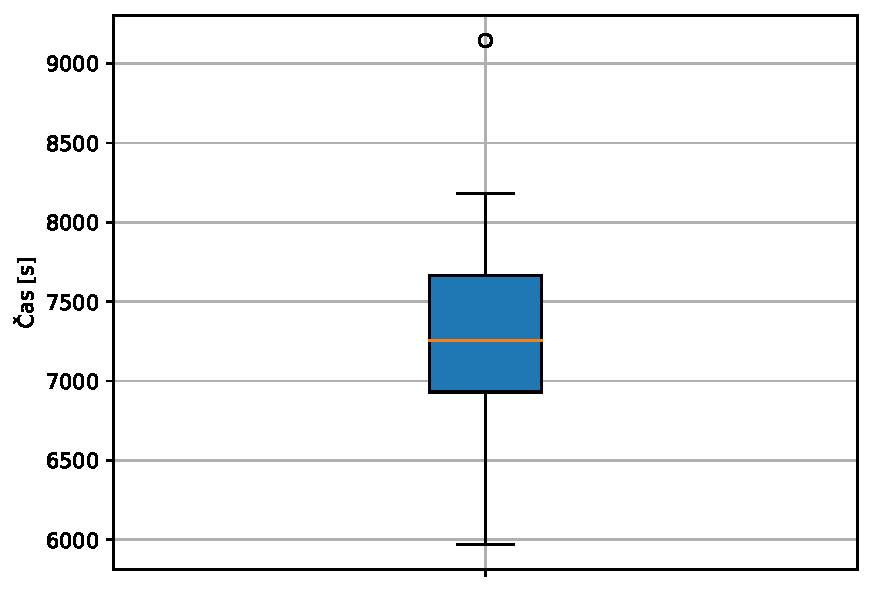
\includegraphics[width=\linewidth]{obrazky-figures/statistics/HIFU/blob/4/SA/timeBoxplot_WithOutliers.pdf}
\caption{Boxplot času potřebného k~dokončení optimalizace ve vteřinách. ($7200s = 2h$)}
\label{fg:hifu:sa:time}
\end{minipage}
\end{figure}



\subsubsection{Tabu prohledávání}
Výsledky tabu prohledávání se zdají být objektivně horší, než výsledky simulovaného žíhání; jediným dalším zkoumaným optimalizačním algoritmem, který nevyužívá populace. Zdá se, že TS vyžaduje více evaluací a nebo uvázlo v~lokálním minimu. Je nutné podotknout, že tato implementace pracuje pouze s~dlouhodobým seznamem. Přidání dalších paměťových struktur by pravděpodobně urychlilo konvergenci a~vylepšilo i~globálnost algoritmu. Na grafu~\ref{fg:hifu:tabu:lastGen} lze vidět rozdíl mezi SA a TS - tabu prohledávání nepokrylo ani zdaleka tak velký rozptyl fitness, jako simulované žíhání. 

\begin{figure}[H]
\begin{minipage}[t]{0.475\linewidth}
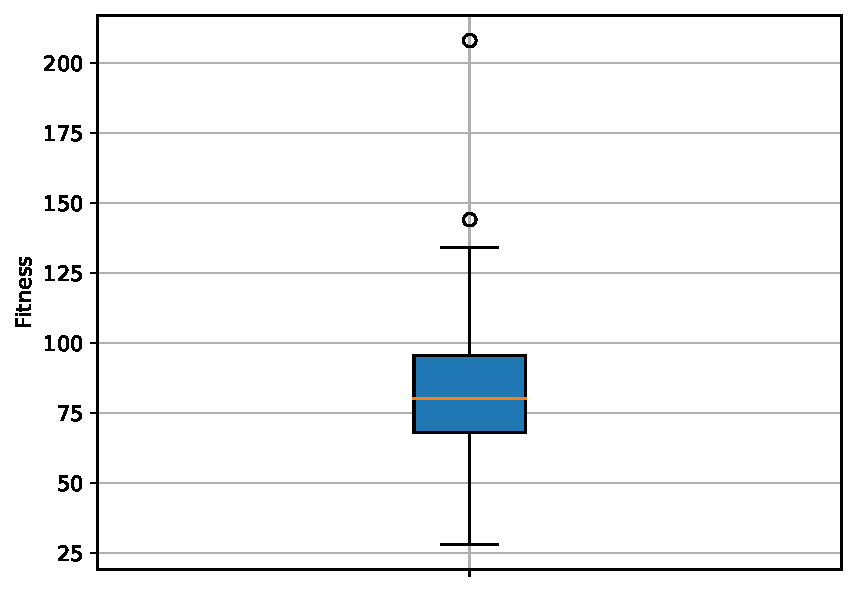
\includegraphics[width=\linewidth]{obrazky-figures/statistics/HIFU/blob/4/TABU/bestsBoxplot_WithOutliers.pdf}
\caption{Boxplot nejlepších výsledků všech $15$ běhů TABU.}
\label{fg:hifu:tabu:best}
\end{minipage}
\hfill
\begin{minipage}[t]{0.475\linewidth}
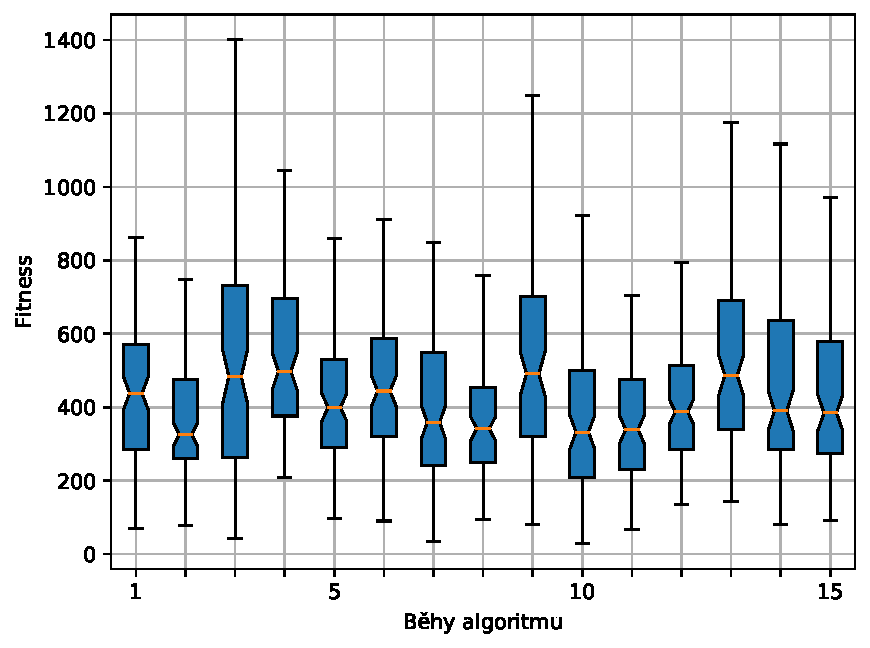
\includegraphics[width=\linewidth]{obrazky-figures/statistics/HIFU/blob/4/TABU/lastGenBoxplots.pdf}
\caption{Boxplot ukazující rozptyl fitness, jaký každý běh TABU prohledal.}
\label{fg:hifu:tabu:lastGen}
\end{minipage}
\end{figure}

\begin{figure}[H]
\begin{minipage}[t]{0.475\linewidth}
	\includegraphics[width=\textwidth]{obrazky-figures/statistics/HIFU/blob/4/TABU/bestsToFitness_1.pdf}
	\caption{Poměr mediánu nejlepších nalezených řešení vůči počtu evaluací fitness funkce.  Zobrazena až druhá poloviny optimalizace.}
	\label{fg:hifu:tabu:fitPerf}
\end{minipage}
\hfill
\begin{minipage}[t]{0.475\linewidth}
\includegraphics[width=\linewidth]{obrazky-figures/statistics/HIFU/blob/4/TABU/timeBoxplot_WithOutliers.pdf}
\caption{Boxplot času potřebného k~dokončení optimalizace ve vteřinách. ($7200s = 2h$)}
\label{fg:hifu:tabu:time}
\end{minipage}
\end{figure}


\subsubsection{Diferenciální evoluce}
Diferenciální evoluce se zdá být lepší, než simulované žíhání. Mohlo by se zdát, že se zde stále vyskytuje problém, který se objevil při optimalizace testovacích funkcí - algoritmus nedokončil konvergenci. Populace se jeví být po dokončení stále různorodá a docházelo k~pravidelnému vylepšení nejlepšího řešení i několik generací před ukončením - viz grafy~\ref{fg:hifu:de:evoProg}. Pokud budeme tento graf studovat detailněji, zjistíme, že je možné pozorovat vliv strategie \emph{best/1/bin} - algoritmus vylepšuje populaci za použití nejlepšího jedince a medián se tedy přibližuje nejlepšímu řešení. Šlo by tedy předpovědět, že by netrvalo příliš mnoho generací, než by populace degenerovala.

\begin{figure}[H]
\begin{minipage}[t]{0.475\linewidth}
\includegraphics[width=\linewidth]{obrazky-figures/statistics/HIFU/blob/4/DE/bestsBoxplot_WithOutliers.pdf}
\caption{Boxplot nejlepších výsledků všech $15$ běhů DE.}
\label{fg:hifu:de:best}
\end{minipage}
\hfill
\begin{minipage}[t]{0.475\linewidth}
\includegraphics[width=\linewidth]{obrazky-figures/statistics/HIFU/blob/4/DE/lastGenBoxplots.pdf}
\caption{Boxplot stavu poslední generace všech $15$ běhů DE. Zvláštní konce ve tvaru vidlice indikují, že medián je příliš blízko kvartálu. Typicky předzvěst degenerace či indikátor příliš malé velikosti populace. }
\label{fg:hifu:de:lastGen}
\end{minipage}
\end{figure}


\begin{figure}[H]
\begin{minipage}[t]{0.475\linewidth}
	\includegraphics[width=\textwidth]{obrazky-figures/statistics/HIFU/blob/4/DE/bestsToFitness_1.pdf}
	\caption{Poměr mediánu nejlepších nalezených řešení vůči počtu evaluací fitness funkce. Zobrazena až druhá poloviny optimalizace.}
	\label{fg:hifu:de:fitPerf}
\end{minipage}
\hfill
\begin{minipage}[t]{0.475\linewidth}
\includegraphics[width=\linewidth]{obrazky-figures/statistics/HIFU/blob/4/DE/timeBoxplot_WithOutliers.pdf}
\caption{Boxplot času potřebného k~dokončení optimalizace ve vteřinách. ($7200s = 2h$)}
\label{fg:hifu:de:time}
\end{minipage}
\end{figure}

\begin{figure}[H]
    \makebox[\textwidth][c]{
    \begin{tabular}{cc}
	\includegraphics[width=75mm]{obrazky-figures/statistics/HIFU/blob/4/DE/evolutionProgress_0.pdf}
    &
	\includegraphics[width=75mm]{obrazky-figures/statistics/HIFU/blob/4/DE/evolutionProgress_1.pdf}
    &
	\includegraphics[width=75mm]{obrazky-figures/statistics/HIFU/blob/4/DE/evolutionProgress_2.pdf}
    &
	\includegraphics[width=75mm]{obrazky-figures/statistics/HIFU/blob/4/DE/evolutionProgress_3.pdf}
    \end{tabular}
    }
    \caption{Data jsou mediány ze všech běhů v~konkrétních generacích. Graf rozdělen na čtvrtiny pro větší detail. Body ukazují medián nejlepších a nejhorších nalezených řešení v~dané generaci.}
    \label{fg:hifu:de:evoProg}
\end{figure}



\subsubsection{Optimalizace rojem částic}
Výkon PSO je dostatečný. Podle grafu poslední generace~\ref{fg:hifu:pso:lastGen} lze soudit, že populace byly dostatečně různorodé a metoda pouze ve většině případů nestihla konvergovat.
\begin{figure}[H]
\begin{minipage}[t]{0.475\linewidth}
\includegraphics[width=\linewidth]{obrazky-figures/statistics/HIFU/blob/4/PSO/bestsBoxplot_WithOutliers.pdf}
\caption{Boxplot nejlepších výsledků všech $15$ běhů PSO.}
\label{fg:hifu:pso:best}
\end{minipage}
\hfill
\begin{minipage}[t]{0.475\linewidth}
\includegraphics[width=\linewidth]{obrazky-figures/statistics/HIFU/blob/4/PSO/lastGenBoxplots.pdf}
\caption{Boxplot stavu poslední generace všech $15$ běhů PSO. Zvláštní konce ve tvaru vidlice indikují, že medián je příliš blízko kvartálu. Typicky předzvěst degenerace či indikátor příliš malé velikosti populace. }
\label{fg:hifu:pso:lastGen}
\end{minipage}
\end{figure}


\begin{figure}[H]

\begin{minipage}[t]{0.475\linewidth}
	\includegraphics[width=\textwidth]{obrazky-figures/statistics/HIFU/blob/4/PSO/bestsToFitness_1.pdf}
	\caption{Poměr mediánu nejlepších nalezených řešení vůči počtu evaluací fitness funkce. Zobrazena až druhá poloviny optimalizace.}
	\label{fg:hifu:pso:fitPerf}
\end{minipage}
\hfill
\begin{minipage}[t]{0.475\linewidth}
\includegraphics[width=\linewidth]{obrazky-figures/statistics/HIFU/blob/4/PSO/timeBoxplot_WithOutliers.pdf}
\caption{Boxplot času potřebného k~dokončení optimalizace ve vteřinách. ($7200s = 2h$)}
\label{fg:hifu:pso:time}
\end{minipage}
\end{figure}

\begin{figure}[H]
    \makebox[\textwidth][c]{
    \begin{tabular}{cc}
	\includegraphics[width=75mm]{obrazky-figures/statistics/HIFU/blob/4/PSO/evolutionProgress_0.pdf}
    &
	\includegraphics[width=75mm]{obrazky-figures/statistics/HIFU/blob/4/PSO/evolutionProgress_1.pdf}
    &
	\includegraphics[width=75mm]{obrazky-figures/statistics/HIFU/blob/4/PSO/evolutionProgress_2.pdf}
    &
	\includegraphics[width=75mm]{obrazky-figures/statistics/HIFU/blob/4/PSO/evolutionProgress_3.pdf}
    \end{tabular}
    }
    \caption{Data jsou mediány ze všech běhů v~konkrétních generacích. Graf rozdělen na čtvrtiny pro větší detail. Body ukazují medián nejlepších a nejhorších nalezených řešení v~dané generaci.}
    \label{fg:hifu:pso:evoProg}
\end{figure}



\subsubsection{CMA-ES}
CMA-ES jako jediné dokázalo najít hledané optimum~(~\ref{fg:hifu:cmaes:best}~). Navíc toho docílilo i před využitím všech $2000$ fitness evaluací~ (~\ref{fg:hifu:cmaes:fitPerf}~). Na grafu~\ref{fg:hifu:cmaes:fitPerf} je možné pozorovat ostré skoky způsobenou průměrovou povahu algoritmu. Metoda vytváří nové populace na základě doposud nalezených statistických distribucí pro jednotlivé proměnné, což může při příliš vysoké deviaci způsobit právě tento profil pohybu mediánu populace.

\begin{figure}[H]
    \begin{minipage}[t]{0.475\linewidth}
        \includegraphics[width=\linewidth]{obrazky-figures/statistics/HIFU/blob/4/CMAES/bestsBoxplot_WithOutliers.pdf}
        \caption{Boxplot nejlepších výsledků všech $15$ běhů CMA-ES.}
        \label{fg:hifu:cmaes:best}
        \end{minipage}
        \hfill
        \begin{minipage}[t]{0.475\linewidth}
        \includegraphics[width=\linewidth]{obrazky-figures/statistics/HIFU/blob/4/CMAES/lastGenBoxplots.pdf}
        \caption{Boxplot stavu poslední generace všech $15$ běhů CMA-ES. Zvláštní konce ve tvaru vidlice indikují, že medián je příliš blízko kvartálu. Typicky předzvěst degenerace či indikátor příliš malé velikosti populace. }
        \label{fg:hifu:cmaes:lastGen}
    \end{minipage}
\end{figure}

\begin{figure}[H]
    \begin{minipage}[t]{0.475\linewidth}
    	\includegraphics[width=\textwidth]{obrazky-figures/statistics/HIFU/blob/4/CMAES/bestsToFitness_1.pdf}
    	\caption{Poměr mediánu nejlepších nalezených řešení vůči počtu evaluací fitness funkce. Zobrazena až druhá poloviny optimalizace.}
    	\label{fg:hifu:cmaes:fitPerf}
    \end{minipage}
    \hfill
    \begin{minipage}[t]{0.475\linewidth}
        \includegraphics[width=\linewidth]{obrazky-figures/statistics/HIFU/blob/4/CMAES/timeBoxplot_WithOutliers.pdf}
        \caption{Boxplot času potřebného k~dokončení optimalizace ve vteřinách. ($7200s = 2h$)}
        \label{fg:hifu:cmaes:time}
    \end{minipage}
\end{figure}

\begin{figure}[H]
    \makebox[\textwidth][c]{
    \begin{tabular}{cc}
	\includegraphics[width=75mm]{obrazky-figures/statistics/HIFU/blob/4/CMAES/evolutionProgress_0.pdf}
    &
	\includegraphics[width=75mm]{obrazky-figures/statistics/HIFU/blob/4/CMAES/evolutionProgress_1.pdf}
    &


	\includegraphics[width=75mm]{obrazky-figures/statistics/HIFU/blob/4/CMAES/evolutionProgress_2.pdf}
    &

	\includegraphics[width=75mm]{obrazky-figures/statistics/HIFU/blob/4/CMAES/evolutionProgress_3.pdf}

    \end{tabular}
    }
    \caption{Data jsou mediány ze všech běhů v~konkrétních generacích. Graf rozdělen na čtvrtiny pro větší detail. Body ukazují medián nejlepších a nejhorších nalezených řešení v~dané generaci.}
    \label{fg:hifu:cmaes:evoProg}
\end{figure}

\subsubsection{Souhrn}
Tato sekce prezentuje grafy pro porovnání výsledků jednotlivých metod. Graf~\ref{fg:hifu:all:best} porovnává nejlepší výsledky nalezené jednotlivými metodami. Z~grafu je patrné, že nejlepším algoritmem se ukázala metoda \textbf{CMA-ES}. Jedním z~hlavních důvodů je pravděpodobně skutečnost, že nevyžaduje nastavování parametrů. Tato metoda navíc vznikla právě se zaměřením na optimalizaci více-dimenzionálních problémů. Nejhůře dopadlo tabu prohledávání a genetický algoritmus. \textbf{Tabu prohledávání} využívalo pouze dlouhodobé paměti předchozích stavů a je pravděpodobné, že $16$ dimenzí problému bylo příliš mnoho, aby byl takovýto seznam efektivní. \textbf{Genetický algoritmus} trpí problémy s~různorodostí populace a omezením maximálního počtu evaluací fitness funkce. \textbf{Simulované žíhání} se ukazuje jako efektivní kompromis. Zdá se, že lineární chladící rozvrh je vhodnou variantou. \textbf{Diferenciální evoluce} je i zde, stejně jako u~testovacích funkcí, na druhém místě. Spolu s~\textbf{PSO} má příliš pomalou konvergenci. Dále; přestože PSO má horší médián výsledků, notche zařadí tyto výsledky s~95\% jistotou na stejnou úroveň, jako DE a SA (a také GA, které je ovšem prokazatelně odlišné od SA a DE). 

Vizualizaci nejlepšího nalezeného výsledku je možné vidět v~přílohách na obrázku~\ref{fg:hifu:prog}.

\begin{figure}[H]
    \centering
    \includegraphics[width=0.6\linewidth]{obrazky-figures/statistics/HIFU/blob/4/JOINED/solutionsPlotsComparasion.pdf}
    \caption{Porovnání výsledků všech algoritmů pro malé množství sonikací.}
    \label{fg:hifu:all:best}
\end{figure}        

\subsection{Skvrna - vysoký počet sonikací}
Optimalizace byly spuštěny s~následujícími řídícími parametry. Došlo k~menším úpravám na základě znalostí získaných při optimalizaci s~malým počtem sonikací.

\begin{table}[H]
\centering
\resizebox{\textwidth}{!}{%
\begin{tabular}{|c|c|c|c|c|c|}
\hline
\multirow{3}{*}{\textbf{GA}} &
  \multirow{3}{*}{\begin{tabular}[c]{@{}c@{}}64 jedinců \\ v~populaci\end{tabular}} &
  \multirow{3}{*}{\begin{tabular}[c]{@{}c@{}}Turnajový \\ výběr\end{tabular}} &
  \multirow{3}{*}{\begin{tabular}[c]{@{}c@{}}Dvoubodové \\ křížení 80\%\end{tabular}} &
  \multirow{3}{*}{\begin{tabular}[c]{@{}c@{}}Mutace \\ 20\%\end{tabular}} &
  \multirow{3}{*}{\begin{tabular}[c]{@{}c@{}}Přežití nejlepších \\ bez ohledu \\ na generaci\end{tabular}} \\
 &
   &
   &
   &
   &
   \\
 &
   &
   &
   &
   &
   \\ \hline
\multirow{2}{*}{\textbf{SA}} &
  \multirow{2}{*}{\begin{tabular}[c]{@{}c@{}}Počáteční \\ teplota 2000\end{tabular}} &
  \multirow{2}{*}{Krok 1\%} &
  \multicolumn{3}{c|}{\multirow{2}{*}{Lineární chladící rozvrh}} \\
 &
   &
   &
  \multicolumn{3}{c|}{} \\ \hline
\textbf{Tabu} &
  \begin{tabular}[c]{@{}c@{}}60 prvků \\ v~tabu seznamu\end{tabular} &
  \multicolumn{4}{c|}{20 kandidátních řešení} \\ \hline
\textbf{DE} &
  \begin{tabular}[c]{@{}c@{}}25 jedinců \\ v~populaci\end{tabular} &
  \begin{tabular}[c]{@{}c@{}}Strategie \\ BEST/1/BIN\end{tabular} &
  \begin{tabular}[c]{@{}c@{}}Šance rekombinace \\ 90\%\end{tabular} &
  \multicolumn{2}{c|}{\begin{tabular}[c]{@{}c@{}}Faktor zesílení \\ 0.5 až 0.9\end{tabular}} \\ \hline
\textbf{PSO} &
  64 částic &
  \multicolumn{2}{c|}{\begin{tabular}[c]{@{}c@{}}Akcelerační koeficienty \\ c1 = c2 = 2\end{tabular}} &
  \multicolumn{2}{c|}{\begin{tabular}[c]{@{}c@{}}Koeficient \\ setrvačnosti 0.5\end{tabular}} \\ \hline
\textbf{\begin{tabular}[c]{@{}c@{}}CMA\\   ES\end{tabular}} &
  \multicolumn{5}{c|}{\textit{Nevyžaduje vstupní parametry.}} \\ \hline
\end{tabular}%
}
\caption{Tabulka řídících parametrů použitých při optimalizaci modelu skvrna vysokým počtem sonikací.}
\end{table}

\subsubsection{Genetický algoritmus}
S~rostoucí dimenzí roste i schopnost GA udržet si diverzitu. Genetický algoritmus byl schopný přiblížit se optimu a populace již nedegenerují - graf~\ref{fg:hifu:blob:ga:lastGen}. Nejlepší řešení se ovšem nacházelo mimo \uv{vousky} boxplotu poslední generace a nelze tedy vyloučit, že se jedná o~náhodu.
\begin{figure}[H]
\begin{minipage}[t]{0.475\linewidth}
\includegraphics[width=\linewidth]{obrazky-figures/statistics/HIFU/blob/20/GA/bestsBoxplot_WithOutliers.pdf}
\caption{Boxplot nejlepších výsledků všech $15$ běhů GA.}
\label{fg:hifu:blob:ga:best}
\end{minipage}
\hfill
\begin{minipage}[t]{0.475\linewidth}
\includegraphics[width=\linewidth]{obrazky-figures/statistics/HIFU/blob/20/GA/lastGenBoxplots.pdf}
\caption{Boxplot stavu poslední generace všech $15$ běhů GA.}
\label{fg:hifu:blob:ga:lastGen}
\end{minipage}
\end{figure}


\begin{figure}[H]
\begin{minipage}[t]{0.475\linewidth}
	\includegraphics[width=\textwidth]{obrazky-figures/statistics/HIFU/blob/20/GA/bestsToFitness_1.pdf}
	\caption{Poměr mediánu nejlepších nalezených řešení vůči počtu evaluací fitness funkce. Zobrazena až druhá poloviny optimalizace.}
	\label{fg:hifu:blob:ga:fitPerf}
\end{minipage}
\hfill
\begin{minipage}[t]{0.475\linewidth}
\includegraphics[width=\linewidth]{obrazky-figures/statistics/HIFU/blob/20/GA/timeBoxplot_WithOutliers.pdf}
\caption{Boxplot času potřebného k~dokončení optimalizace ve vteřinách. ($28800 = 8h$)}
\label{fg:hifu:blob:ga:time}
\end{minipage}
\end{figure}

\begin{figure}[H]
    \makebox[\textwidth][c]{
    \begin{tabular}{cc}
	\includegraphics[width=75mm]{obrazky-figures/statistics/HIFU/blob/20/GA/evolutionProgress_0.pdf}
    &
	\includegraphics[width=75mm]{obrazky-figures/statistics/HIFU/blob/20/GA/evolutionProgress_1.pdf}
    &
	\includegraphics[width=75mm]{obrazky-figures/statistics/HIFU/blob/20/GA/evolutionProgress_2.pdf}
    &
	\includegraphics[width=75mm]{obrazky-figures/statistics/HIFU/blob/20/GA/evolutionProgress_3.pdf}
    \end{tabular}
    }
    \caption{Evoluční průběh GA. Data jsou mediány ze všech běhů v~konkrétních generacích. Graf rozdělen na čtvrtiny pro větší detail. Body ukazují medián nejlepších a nejhorších nalezených řešení v~dané generaci.}
    \label{fg:hifu:blob:ga:evoProg}
\end{figure}



\subsubsection{Simulované žíhání}
Simulované žíhání bylo i zde úspěšné. Zdá se, že zvýšení dimenze problému nemělo příliš velký vliv na schopnosti algoritmu. Navíc vylepšení fitness probíhalo i těsně před ukončením optimalizace - graf~\ref{fg:hifu:blob:sa:fitPerf} - a lze tedy předpokládat, že přidáním dalších evaluací by bylo nalezeno lepší řešení.

\begin{figure}[H]
\begin{minipage}[t]{0.475\linewidth}
\includegraphics[width=\linewidth]{obrazky-figures/statistics/HIFU/blob/20/SA/bestsBoxplot_WithOutliers.pdf}
\caption{Boxplot nejlepších výsledků všech $15$ běhů SA.}
\label{fg:hifu:blob:sa:best}
\end{minipage}
\hfill
\begin{minipage}[t]{0.475\linewidth}
\includegraphics[width=\linewidth]{obrazky-figures/statistics/HIFU/blob/20/SA/lastGenBoxplots.pdf}
\caption{Boxplot ukazující rozptyl fitness, jaký každý běh SA prohledal.}
\label{fg:hifu:blob:sa:lastGen}
\end{minipage}
\end{figure}

\begin{figure}[H]
\begin{minipage}[t]{0.475\linewidth}
	\includegraphics[width=\textwidth]{obrazky-figures/statistics/HIFU/blob/20/SA/bestsToFitness_1.pdf}
	\caption{Poměr mediánu nejlepších nalezených řešení vůči počtu evaluací fitness funkce.  Zobrazena až druhá poloviny optimalizace.}
	\label{fg:hifu:blob:sa:fitPerf}
\end{minipage}
\hfill
\begin{minipage}[t]{0.475\linewidth}
\includegraphics[width=\linewidth]{obrazky-figures/statistics/HIFU/blob/20/SA/timeBoxplot_WithOutliers.pdf}
\caption{Boxplot času potřebného k~dokončení optimalizace ve vteřinách. ($28800s = 8h$)}
\label{fg:hifu:blob:sa:time}
\end{minipage}
\end{figure}



\subsubsection{Tabu prohledávání}
Tabu prohledávání byla jedna z~metod, které byly upraveny řídící parametry, jako pokus vylepšit výkon. Z~výsledků~\ref{fg:hifu:blob:tabu:lastGen} a~\ref{fg:hifu:blob::fitPerf} se ovšem zdá, že bez většího efektu. Stále nevykazuje tak dobré výsledky, jako přímý rival v~algoritmu Simulovaného žíhání. Závěr o~TS z~předchozího testu stále platí - vyžaduje více evaluací a nebo uvázlo v~lokálním minimu. Také stále platí dodatek, že tato implementace pracuje pouze s~dlouhodobým seznamem. Jedná se o~omezení samotné implementace.

\begin{figure}[H]
\begin{minipage}[t]{0.475\linewidth}
\includegraphics[width=\linewidth]{obrazky-figures/statistics/HIFU/blob/20/TABU/bestsBoxplot_WithOutliers.pdf}
\caption{Boxplot nejlepších výsledků všech $15$ běhů TABU.}
\label{fg:hifu:blob:tabu:best}
\end{minipage}
\hfill
\begin{minipage}[t]{0.475\linewidth}
\includegraphics[width=\linewidth]{obrazky-figures/statistics/HIFU/blob/20/TABU/lastGenBoxplots.pdf}
\caption{Boxplot ukazující rozptyl fitness, jaký každý běh TABU prohledal.}
\label{fg:hifu:blob:tabu:lastGen}
\end{minipage}
\end{figure}

\begin{figure}[H]
\begin{minipage}[t]{0.475\linewidth}
	\includegraphics[width=\textwidth]{obrazky-figures/statistics/HIFU/blob/20/TABU/bestsToFitness_1.pdf}
	\caption{Poměr mediánu nejlepších nalezených řešení vůči počtu evaluací fitness funkce.  Zobrazena až druhá poloviny optimalizace.}
	\label{fg:hifu:blob::fitPerf}
\end{minipage}
\hfill
\begin{minipage}[t]{0.475\linewidth}
\includegraphics[width=\linewidth]{obrazky-figures/statistics/HIFU/blob/20/TABU/timeBoxplot_WithOutliers.pdf}
\caption{Boxplot času potřebného k~dokončení optimalizace ve vteřinách. ($28800s = 8h$)}
\label{fg:hifu:blob:tabu:time}
\end{minipage}
\end{figure}


\subsubsection{Diferenciální evoluce}
Diferenciální evoluce vykazuje markantní zhoršení výsledků se zvýšením dimenze. Z~grafu~\ref{fg:hifu:blob:de:fitPerf} a~\ref{fg:hifu:blob:de:evoProg} se zdá, že došlo k~uváznutí ještě před $1300$ evaluacemi účelové funkce. Jak bylo dříve zmíněno, řetěz sonikací v~různých pořadích mohou mít stejnou fitness. Například řetěz, který vypálí všechny cílené body ovšem zároveň s~nimi i část penalizované mapy. Dokážeme si představit, že takových řetězů může být v~populací obecně více, každý zasahující na jinou část penalizační mapy. Rekombinací těchto řešení pravděpodobně vznikne řešení horší, což značně stěžuje schopnost algoritmu konvergovat při strategiích využívajících pouze fitness jako selekční tlak. Je možné, že strategie \emph{rand}, či jiná, pracující s~náhodnými prvky, by mohla zvýšit globálnost.

\begin{figure}[H]
\begin{minipage}[t]{0.475\linewidth}
\includegraphics[width=\linewidth]{obrazky-figures/statistics/HIFU/blob/20/DE/bestsBoxplot_WithOutliers.pdf}
\caption{Boxplot nejlepších výsledků všech $15$ běhů DE.}
\label{fg:hifu:blob:de:best}
\end{minipage}
\hfill
\begin{minipage}[t]{0.475\linewidth}
\includegraphics[width=\linewidth]{obrazky-figures/statistics/HIFU/blob/20/DE/lastGenBoxplots.pdf}
\caption{Boxplot stavu poslední generace všech $15$ běhů DE.}
\label{fg:hifu:blob:de:lastGen}
\end{minipage}
\end{figure}


\begin{figure}[H]
\begin{minipage}[t]{0.475\linewidth}
	\includegraphics[width=\textwidth]{obrazky-figures/statistics/HIFU/blob/20/DE/bestsToFitness_1.pdf}
	\caption{Poměr mediánu nejlepších nalezených řešení vůči počtu evaluací fitness funkce. Zobrazena až druhá poloviny optimalizace.}
	\label{fg:hifu:blob:de:fitPerf}
\end{minipage}
\hfill
\begin{minipage}[t]{0.475\linewidth}
\includegraphics[width=\linewidth]{obrazky-figures/statistics/HIFU/blob/20/DE/timeBoxplot_WithOutliers.pdf}
\caption{Boxplot času potřebného k~dokončení optimalizace ve vteřinách. ($28800s = 8h$)}
\label{fg:hifu:blob:de:time}
\end{minipage}
\end{figure}

\begin{figure}[H]
    \makebox[\textwidth][c]{
    \begin{tabular}{cc}
	\includegraphics[width=75mm]{obrazky-figures/statistics/HIFU/blob/20/DE/evolutionProgress_0.pdf}
    &
	\includegraphics[width=75mm]{obrazky-figures/statistics/HIFU/blob/20/DE/evolutionProgress_1.pdf}
    &
	\includegraphics[width=75mm]{obrazky-figures/statistics/HIFU/blob/20/DE/evolutionProgress_2.pdf}
    &
	\includegraphics[width=75mm]{obrazky-figures/statistics/HIFU/blob/20/DE/evolutionProgress_3.pdf}
    \end{tabular}
    }
    \caption{Data jsou mediány ze všech běhů v~konkrétních generacích. Graf rozdělen na čtvrtiny pro větší detail. Body ukazují medián nejlepších a nejhorších nalezených řešení v~dané generaci.}
    \label{fg:hifu:blob:de:evoProg}
\end{figure}



\subsubsection{Optimalizace rojem částic}
Dalším zklamáním po zvýšení dimenze problému je metoda PSO. Optimalizace rojem částic má spolu s~metodou DE ve strategii \emph{best} společnou důležitou vlastnost - svou populaci přibližuje k~nějakému podprostoru, na základě směru vypočteném z~nejlepších řešení. V~případě, že v~populaci existuje více přibližně stejných nejlepších řešení zakódovaných výrazně odlišně, algoritmus postrádá schopnost konvergovat. Multi-swarm by mohl tento problém vyřešit.

\begin{figure}[H]
\begin{minipage}[t]{0.475\linewidth}
\includegraphics[width=\linewidth]{obrazky-figures/statistics/HIFU/blob/20/PSO/bestsBoxplot_WithOutliers.pdf}
\caption{Boxplot nejlepších výsledků všech $15$ běhů PSO.}
\label{fg:hifu:blob:pso:best}
\end{minipage}
\hfill
\begin{minipage}[t]{0.475\linewidth}
\includegraphics[width=\linewidth]{obrazky-figures/statistics/HIFU/blob/20/PSO/lastGenBoxplots.pdf}
\caption{Boxplot stavu poslední generace všech $15$ běhů PSO.}
\label{fg:hifu:blob:pso:lastGen}
\end{minipage}
\end{figure}


\begin{figure}[H]

\begin{minipage}[t]{0.475\linewidth}
	\includegraphics[width=\textwidth]{obrazky-figures/statistics/HIFU/blob/20/PSO/bestsToFitness_1.pdf}
	\caption{Poměr mediánu nejlepších nalezených řešení vůči počtu evaluací fitness funkce. Zobrazena až druhá poloviny optimalizace.}
	\label{fg:hifu:blob:pso:fitPerf}
\end{minipage}
\hfill
\begin{minipage}[t]{0.475\linewidth}
\includegraphics[width=\linewidth]{obrazky-figures/statistics/HIFU/blob/20/PSO/timeBoxplot_WithOutliers.pdf}
\caption{Boxplot času potřebného k~dokončení optimalizace ve vteřinách. ($28800s = 8h$)}
\label{fg:hifu:blob:pso:time}
\end{minipage}
\end{figure}

\begin{figure}[H]
    \makebox[\textwidth][c]{
    \begin{tabular}{cc}
	\includegraphics[width=75mm]{obrazky-figures/statistics/HIFU/blob/20/PSO/evolutionProgress_0.pdf}
    &
	\includegraphics[width=75mm]{obrazky-figures/statistics/HIFU/blob/20/PSO/evolutionProgress_1.pdf}
    &
	\includegraphics[width=75mm]{obrazky-figures/statistics/HIFU/blob/20/PSO/evolutionProgress_2.pdf}
    &
	\includegraphics[width=75mm]{obrazky-figures/statistics/HIFU/blob/20/PSO/evolutionProgress_3.pdf}
    \end{tabular}
    }
    \caption{Data jsou mediány ze všech běhů v~konkrétních generacích. Graf rozdělen na čtvrtiny pro větší detail. Body ukazují medián nejlepších a nejhorších nalezených řešení v~dané generaci.}
    \label{fg:hifu:blob:pso:evoProg}
\end{figure}



\subsubsection{CMA-ES}
I~zde se CMA-ES ukázala jako jediná metoda, schopná konzistentně najít, nebo se alespoň přiblížit, ke hledanému optimu~(~\ref{fg:hifu:cmaes:best}~).

\begin{figure}[H]
    \begin{minipage}[t]{0.475\linewidth}
        \includegraphics[width=\linewidth]{obrazky-figures/statistics/HIFU/blob/20/CMAES/bestsBoxplot_WithOutliers.pdf}
        \caption{Boxplot nejlepších výsledků všech $15$ běhů CMA-ES.}
        \label{fg:hifu:blob:cmaes:best}
        \end{minipage}
        \hfill
        \begin{minipage}[t]{0.475\linewidth}
        \includegraphics[width=\linewidth]{obrazky-figures/statistics/HIFU/blob/20/CMAES/lastGenBoxplots.pdf}
        \caption{Boxplot stavu poslední generace všech $15$ běhů CMA-ES.}
        \label{fg:hifu:blob:cmaes:lastGen}
    \end{minipage}
\end{figure}

\begin{figure}[H]
    \begin{minipage}[t]{0.475\linewidth}
    	\includegraphics[width=\textwidth]{obrazky-figures/statistics/HIFU/blob/20/CMAES/bestsToFitness_1.pdf}
    	\caption{Poměr mediánu nejlepších nalezených řešení vůči počtu evaluací fitness funkce. Zobrazena až druhá poloviny optimalizace.}
    	\label{fg:hifu:blob:cmaes:fitPerf}
    \end{minipage}
    \hfill
    \begin{minipage}[t]{0.475\linewidth}
        \includegraphics[width=\linewidth]{obrazky-figures/statistics/HIFU/blob/20/CMAES/timeBoxplot_WithOutliers.pdf}
        \caption{Boxplot času potřebného k~dokončení optimalizace ve vteřinách. ($28800s = 8h$)}
        \label{fg:hifu:blob:cmaes:time}
    \end{minipage}
\end{figure}

\begin{figure}[H]
    \makebox[\textwidth][c]{
    \begin{tabular}{cc}
	\includegraphics[width=75mm]{obrazky-figures/statistics/HIFU/blob/20/CMAES/evolutionProgress_0.pdf}
    &
	\includegraphics[width=75mm]{obrazky-figures/statistics/HIFU/blob/20/CMAES/evolutionProgress_1.pdf}
    &


	\includegraphics[width=75mm]{obrazky-figures/statistics/HIFU/blob/20/CMAES/evolutionProgress_2.pdf}
    &

	\includegraphics[width=75mm]{obrazky-figures/statistics/HIFU/blob/20/CMAES/evolutionProgress_3.pdf}

    \end{tabular}
    }
    \caption{Data jsou mediány ze všech běhů v~konkrétních generacích. Graf rozdělen na čtvrtiny pro větší detail. Body ukazují medián nejlepších a nejhorších nalezených řešení v~dané generaci.}
    \label{fg:hifu:blob:cmaes:evoProg}
\end{figure}

\subsubsection{Souhrn}
Grafy~\ref{fg:hifu:blob:joined} jasně ukazují, že i zde vyhrává metoda \textbf{CMA-ES}. Jak již bylo zmíněno, metoda nevyžaduje vstupní řídící parametry a optimalizace více-dimenzionálních problémů je její \uv{forte}. Nejhůře dopadlo \textbf{PSO} a \textbf{Diferenciální evoluce}, pravděpodobně z~důvodu pomalé, nebo i zamrzlé konvergence. Jak bylo zmíněno, obě metody posouvají svou populaci směrem, který je udáván nejlepšími jedinci v~populaci. Pokud je takto silných jedinců v~populaci mnoho a každý udává jiný/opačný směr, algoritmy nekonvergují. Lze předpokládat, že tato situace nastala - algoritmus dokázal odstranit celou cílenou část, ovšem za cenu velké penalizace zasažením zakázaných oblastí. \textbf{Tabu prohledávání} je i nadále horší než \textbf{Simulované žíhání}, které se zdá být invariantní vůči dimenzi problému. Naopak \textbf{Genetický algoritmus} byl díky zvýšení dimenze schopen překonat problémy s~diverzitou a~velice rychle se posunul směrem k~optimu. 
Vizualizaci nejlepšího nalezeného výsledku je možné vidět v~přílohách na obrázku~\ref{fg:hifu:blob:prog}.

\begin{figure}[H]
    \makebox[\textwidth][c]{
    \begin{tabular}{cc}
	\includegraphics[width=75mm]{obrazky-figures/statistics/HIFU/blob/20/JOINED/solutionsPlotsComparasion.pdf}
    &
	\includegraphics[width=75mm]{obrazky-figures/statistics/HIFU/blob/20/JOINED/detail_solutionsPlotsComparasion.pdf}
    \end{tabular}
    }
    \caption{Porovnání výsledků všech algoritmů pro $20$ sonikací. Vlevo všechny metody, vpravo detail na úspěšnější z~nich.}
    \label{fg:hifu:blob:joined}
\end{figure}


\subsection{Květina}
Pro optimalizaci tvaru květina bylo přistoupeno k~ústupkům vzhledem k~časové náročnosti a předchozím poznatkům. Hlavním z~těchto ústupků je vynechání \textbf{Tabu prohledávání} a \textbf{Optimalizace rojem částic}. Ani jeden z~těchto algoritmů nebyl schopen překonat svého přímého konkurenta (Simulované žíhání a Diferenciální evoluci resp.). Další z~ústupků plyne ze znalosti kvality výsledků a časové náročnosti výpočtů - každému algoritmu bylo provedeno pouze $10$ nezávislých běhů, namísto předchozích $15$, z~důvodu šetření procesorových hodin. Model květina je složitějším problémem, než skrvna především z~důvodu reziduálního akumulovaného tepla ve středu modelu. Pro úsporu času bylo také použito $15$, namísto předešlých $20$ sonikací. Částečné řešení problému reziduálního tepla je možné za pomoci vysokých hodnot proměnné $t_{off}$ v~rámci sonikací. Vysoké hodnoty mají ovšem za následek delší simulace, které při původních $20$ sonikacích přesáhli hranici $12$ hodin na superpočítači. Takto nalezené řešení by nesplnilo dříve představena kritéria na včasnost výsledků.

Optimalizace byly spuštěny s~následujícími řídícími parametry.

\begin{table}[H]
\centering
\resizebox{\textwidth}{!}{%
\begin{tabular}{|c|c|c|c|c|c|}
\hline
\multirow{3}{*}{\textbf{GA}} &
  \multirow{3}{*}{\begin{tabular}[c]{@{}c@{}}64 jedinců \\ v~populaci\end{tabular}} &
  \multirow{3}{*}{\begin{tabular}[c]{@{}c@{}}Turnajový \\ výběr\end{tabular}} &
  \multirow{3}{*}{\begin{tabular}[c]{@{}c@{}}Dvoubodové \\ křížení 80\%\end{tabular}} &
  \multirow{3}{*}{\begin{tabular}[c]{@{}c@{}}Mutace \\ 20\%\end{tabular}} &
  \multirow{3}{*}{\begin{tabular}[c]{@{}c@{}}Přežití nejlepších \\ bez ohledu \\ na generaci\end{tabular}} \\
 &
   &
   &
   &
   &
   \\
 &
   &
   &
   &
   &
   \\ \hline
\multirow{2}{*}{\textbf{SA}} &
  \multirow{2}{*}{\begin{tabular}[c]{@{}c@{}}Počáteční \\ teplota 2000\end{tabular}} &
  \multirow{2}{*}{Krok 1\%} &
  \multicolumn{3}{c|}{\multirow{2}{*}{Lineární chladící rozvrh}} \\
 &
   &
   &
  \multicolumn{3}{c|}{} \\ \hline
\textbf{DE} &
  \begin{tabular}[c]{@{}c@{}}25 jedinců \\ v~populaci\end{tabular} &
  \begin{tabular}[c]{@{}c@{}}Strategie \\ BEST/1/BIN\end{tabular} &
  \begin{tabular}[c]{@{}c@{}}Šance rekombinace \\ 90\%\end{tabular} &
  \multicolumn{2}{c|}{\begin{tabular}[c]{@{}c@{}}Faktor zesílení \\ 0.5 až 0.9\end{tabular}} \\ \hline
\textbf{\begin{tabular}[c]{@{}c@{}}CMA\\   ES\end{tabular}} &
  \multicolumn{5}{c|}{\textit{Nevyžaduje vstupní parametry.}} \\ \hline
\end{tabular}%
}
\caption{Tabulka řídících parametrů použitých při optimalizaci modelu květina větším počtem sonikací.}
\end{table}

\subsubsection{Genetický algoritmus}
Genetický algoritmus nedokázal nalézt optimální řešení při omezeném množství evaluací, dokázal ovšem překonat lokální extrémy a přiblížit se. Při pohledu na grafy~\ref{fg:hifu:flower:ga:lastGen} a~\ref{fg:hifu:flower:ga:evoProg} lze ovšem předpokládat, že při případném uvolnění tohoto omezení by GA bylo schopno dále pokračovat a~řešení upřesnit. 
\begin{figure}[H]
\begin{minipage}[t]{0.475\linewidth}
\includegraphics[width=\linewidth]{obrazky-figures/statistics/HIFU/flower/15/GA/bestsBoxplot_WithOutliers.pdf}
\caption{Boxplot nejlepších výsledků všech $10$ běhů GA.}
\label{fg:hifu:flower:ga:best}
\end{minipage}
\hfill
\begin{minipage}[t]{0.475\linewidth}
\includegraphics[width=\linewidth]{obrazky-figures/statistics/HIFU/flower/15/GA/lastGenBoxplots.pdf}
\caption{Boxplot stavu poslední generace všech $10$ běhů GA.}
\label{fg:hifu:flower:ga:lastGen}
\end{minipage}
\end{figure}


\begin{figure}[H]
\begin{minipage}[t]{0.475\linewidth}
	\includegraphics[width=\textwidth]{obrazky-figures/statistics/HIFU/flower/15/GA/bestsToFitness_1.pdf}
	\caption{Poměr mediánu nejlepších nalezených řešení vůči počtu evaluací fitness funkce. Zobrazena až druhá poloviny optimalizace.}
	\label{fg:hifu:flower:ga:fitPerf}
\end{minipage}
\hfill
\begin{minipage}[t]{0.475\linewidth}
\includegraphics[width=\linewidth]{obrazky-figures/statistics/HIFU/flower/15/GA/timeBoxplot_WithOutliers.pdf}
\caption{Boxplot času potřebného k~dokončení optimalizace ve vteřinách. ($28800 = 8h$)}
\label{fg:hifu:flower:ga:time}
\end{minipage}
\end{figure}

\begin{figure}[H]
    \makebox[\textwidth][c]{
    \begin{tabular}{cc}
	\includegraphics[width=75mm]{obrazky-figures/statistics/HIFU/flower/15/GA/evolutionProgress_0.pdf}
    &
	\includegraphics[width=75mm]{obrazky-figures/statistics/HIFU/flower/15/GA/evolutionProgress_1.pdf}
    &
	\includegraphics[width=75mm]{obrazky-figures/statistics/HIFU/flower/15/GA/evolutionProgress_2.pdf}
    &
	\includegraphics[width=75mm]{obrazky-figures/statistics/HIFU/flower/15/GA/evolutionProgress_3.pdf}
    \end{tabular}
    }
    \caption{Evoluční průběh GA. Data jsou mediány ze všech běhů v~konkrétních generacích. Graf rozdělen na čtvrtiny pro větší detail. Body ukazují medián nejlepších a nejhorších nalezených řešení v~dané generaci.}
    \label{fg:hifu:flower:ga:evoProg}
\end{figure}



\subsubsection{Simulované žíhání}
Simulované žíhání bylo nejúspěšnější z~testovaných metod, ovšem samotné výsledky jsou stále neuspokojivé - algoritmus se pohybuje v~okolí optima ale nedokáže konvergovat. Toto chování algoritmus vyznačoval již při předchozích testech. Na vinně je pravděpodobně velikost kroku, která je generována normální distribuční funkcí s~standardní odchylkou $1/5$ rozmezí proměnné, která je právě perturbována. Tento krok se zdá být příliš velký v~pozdějších fázích prohledávání.

\begin{figure}[H]
\begin{minipage}[t]{0.475\linewidth}
\includegraphics[width=\linewidth]{obrazky-figures/statistics/HIFU/flower/15/SA/bestsBoxplot_WithOutliers.pdf}
\caption{Boxplot nejlepších výsledků všech $10$ běhů SA.}
\label{fg:hifu:flower:sa:best}
\end{minipage}
\hfill
\begin{minipage}[t]{0.475\linewidth}
\includegraphics[width=\linewidth]{obrazky-figures/statistics/HIFU/flower/15/SA/lastGenBoxplots.pdf}
\caption{Boxplot ukazující rozptyl fitness, jaký každý běh SA prohledal.}
\label{fg:hifu:flower:sa:lastGen}
\end{minipage}
\end{figure}

\begin{figure}[H]
\begin{minipage}[t]{0.475\linewidth}
	\includegraphics[width=\textwidth]{obrazky-figures/statistics/HIFU/flower/15/SA/bestsToFitness_1.pdf}
	\caption{Poměr mediánu nejlepších nalezených řešení vůči počtu evaluací fitness funkce. Zobrazena až druhá poloviny optimalizace.}
	\label{fg:hifu:flower:sa:fitPerf}
\end{minipage}
\hfill
\begin{minipage}[t]{0.475\linewidth}
\includegraphics[width=\linewidth]{obrazky-figures/statistics/HIFU/flower/15/SA/timeBoxplot_WithOutliers.pdf}
\caption{Boxplot času potřebného k~dokončení optimalizace ve vteřinách. ($28800s = 8h$)}
\label{fg:hifu:flower:sa:time}
\end{minipage}
\end{figure}


\subsubsection{Diferenciální evoluce}
Diferenciální evoluce vykazuje stejné tendence, jako při předchozím testu. Problém reziduálního tepla způsobí, že stavový prostor je plný lokálních extrémů, které se od ostatních jedinců liší především pořadím provedení sonikací. Na grafu~\ref{fg:hifu:flower:de:fitPerf} je vidět, že přibližně od $1500$ evaluací již nedocházelo ke změnám. Pravděpodobně se jedná o~stav, který jako jeden z~mála nezničí prostřední penalizovanou oblast, ovšem ani nedokáže pokrýt cíl.

\begin{figure}[H]
\begin{minipage}[t]{0.475\linewidth}
\includegraphics[width=\linewidth]{obrazky-figures/statistics/HIFU/flower/15/DE/bestsBoxplot_WithOutliers.pdf}
\caption{Boxplot nejlepších výsledků všech $10$ běhů DE.}
\label{fg:hifu:flower:de:best}
\end{minipage}
\hfill
\begin{minipage}[t]{0.475\linewidth}
\includegraphics[width=\linewidth]{obrazky-figures/statistics/HIFU/flower/15/DE/lastGenBoxplots.pdf}
\caption{Boxplot stavu poslední generace všech $10$ běhů DE.}
\label{fg:hifu:flower:de:lastGen}
\end{minipage}
\end{figure}


\begin{figure}[H]
\begin{minipage}[t]{0.475\linewidth}
	\includegraphics[width=\textwidth]{obrazky-figures/statistics/HIFU/flower/15/DE/bestsToFitness_1.pdf}
	\caption{Poměr mediánu nejlepších nalezených řešení vůči počtu evaluací fitness funkce. Zobrazena až druhá poloviny optimalizace.}
	\label{fg:hifu:flower:de:fitPerf}
\end{minipage}
\hfill
\begin{minipage}[t]{0.475\linewidth}
\includegraphics[width=\linewidth]{obrazky-figures/statistics/HIFU/flower/15/DE/timeBoxplot_WithOutliers.pdf}
\caption{Boxplot času potřebného k~dokončení optimalizace ve vteřinách. ($28800s = 8h$)}
\label{fg:hifu:flower:de:time}
\end{minipage}
\end{figure}

\begin{figure}[H]
    \makebox[\textwidth][c]{
    \begin{tabular}{cc}
	\includegraphics[width=75mm]{obrazky-figures/statistics/HIFU/flower/15/DE/evolutionProgress_0.pdf}
    &
	\includegraphics[width=75mm]{obrazky-figures/statistics/HIFU/flower/15/DE/evolutionProgress_1.pdf}
    &
	\includegraphics[width=75mm]{obrazky-figures/statistics/HIFU/flower/15/DE/evolutionProgress_2.pdf}
    &
	\includegraphics[width=75mm]{obrazky-figures/statistics/HIFU/flower/15/DE/evolutionProgress_3.pdf}
    \end{tabular}
    }
    \caption{Data jsou mediány ze všech běhů v~konkrétních generacích. Graf rozdělen na čtvrtiny pro větší detail. Body ukazují medián nejlepších a nejhorších nalezených řešení v~dané generaci.}
    \label{fg:hifu:flower:de:evoProg}
\end{figure}

\subsubsection{CMA-ES}
Tento problém se ukázal jako příliš náročný i pro CMA-ES. Zdá se, že metoda se přeučí na stavy na počátku hledání a není následně schopna řešit pozdější lokální extremy. V~počátečních fázích jsou nalezena lepší řešení kolem hodnot, které jsou dlouho lokálním optimem a metoda bohužel upraví kovariance do stavů, které nejsou schopny při případném úniku nalézt globální optimum.

\begin{figure}[H]
    \begin{minipage}[t]{0.475\linewidth}
        \includegraphics[width=\linewidth]{obrazky-figures/statistics/HIFU/flower/15/CMAES/bestsBoxplot_WithOutliers.pdf}
        \caption{Boxplot nejlepších výsledků všech $10$ běhů CMA-ES.}
        \label{fg:hifu:flower:cmaes:best}
        \end{minipage}
        \hfill
        \begin{minipage}[t]{0.475\linewidth}
        \includegraphics[width=\linewidth]{obrazky-figures/statistics/HIFU/flower/15/CMAES/lastGenBoxplots.pdf}
        \caption{Boxplot stavu poslední generace všech $10$ běhů CMA-ES.}
        \label{fg:hifu:flower:cmaes:lastGen}
    \end{minipage}
\end{figure}

\begin{figure}[H]
    \begin{minipage}[t]{0.475\linewidth}
    	\includegraphics[width=\textwidth]{obrazky-figures/statistics/HIFU/flower/15/CMAES/bestsToFitness_1.pdf}
    	\caption{Poměr mediánu nejlepších nalezených řešení vůči počtu evaluací fitness funkce. Zobrazena až druhá poloviny optimalizace.}
    	\label{fg:hifu:flower:cmaes:fitPerf}
    \end{minipage}
    \hfill
    \begin{minipage}[t]{0.475\linewidth}
        \includegraphics[width=\linewidth]{obrazky-figures/statistics/HIFU/flower/15/CMAES/timeBoxplot_WithOutliers.pdf}
        \caption{Boxplot času potřebného k~dokončení optimalizace ve vteřinách. ($28800s = 8h$)}
        \label{fg:hifu:flower:cmaes:time}
    \end{minipage}
\end{figure}

\begin{figure}[H]
    \makebox[\textwidth][c]{
    \begin{tabular}{cc}
	\includegraphics[width=75mm]{obrazky-figures/statistics/HIFU/flower/15/CMAES/evolutionProgress_0.pdf}
    &
	\includegraphics[width=75mm]{obrazky-figures/statistics/HIFU/flower/15/CMAES/evolutionProgress_1.pdf}
    &


	\includegraphics[width=75mm]{obrazky-figures/statistics/HIFU/flower/15/CMAES/evolutionProgress_2.pdf}
    &

	\includegraphics[width=75mm]{obrazky-figures/statistics/HIFU/flower/15/CMAES/evolutionProgress_3.pdf}

    \end{tabular}
    }
    \caption{Data jsou mediány ze všech běhů v~konkrétních generacích. Graf rozdělen na čtvrtiny pro větší detail. Body ukazují medián nejlepších a nejhorších nalezených řešení v~dané generaci.}
    \label{fg:hifu:flower:cmaes:evoProg}
\end{figure}

\subsubsection{Souhrn}
Grafy~\ref{fg:hifu:blob:joined} ukazují, že ani jeden z~algoritmů nebyl úspěšný při řešení tohoto typu problému. Největším zákoutím je nutnost a tlak na algoritmy vyhnout se střednímu bodu, který je velice snadno spálen díky kladné zpětné vazbě vznikajícího reziduálního tepla při pálení okolí. Genetický algoritmus je příliš omezen kritériem $2000$ evaluací, Diferenciální evoluce uvázne v~lokálním minimu, Simulované žíhání nemá dostatečně flexibilní krok pro přesnou konvergenci a CMA-ES se přeučí na neoptimální počátečním prostředí. Vhodným řešením by mohla být kombinace SA a CMA-ES, při které je prvních $1000$ evaluací použito k~nalezení přibližné pozice optima algoritmem SA a následně výsledek předán CMA-ES jako počáteční stav.
Vizualizaci nejlepšího nalezeného výsledku je možné vidět v~přílohách na obrázku~\ref{fg:hifu:flower:prog}.

\begin{figure}[H]
    \centering
	\includegraphics[width=0.6\linewidth]{obrazky-figures/statistics/HIFU/flower/15/JOINED/solutionsPlotsComparasion.pdf}

    \caption{Porovnání výsledků všech algoritmů pro problém květiny.}
    \label{fg:hifu:flower:joined}
\end{figure}


\section{Shrnutí a přínos pro klinickou praxi}
Bylo bezesporu ukázáno, že pro problém připomínající typ \uv{skvrna} je nejvhodnějším kandidátem algoritmus \textbf{CMA-ES}. Splňuje kritéria včasnosti výpočtu i přesnosti - jako jediný byl schopen nalézt optimum ve vymezeném rozsahu evaluací. Problém typu \uv{květina} nebyl řešitelný v~rámci definovaných kritérii - nepodařilo se nalézt optimum. Pro přibližné řešení tohoto typu oblasti je ovšem možné využít algoritmu \textbf{Simulované žíhání}.

Hlavním rysem obou metod je menší množství vstupních parametrů, případně citlivost metody na tyto parametry. Přejeme-li si najít vhodnou evoluční metodu pro řešení problému hledání trajektorie HIFU operací, jedná se o~žádaný efekt. Platí \uv{no-free-lunch} teorém a problém je závislý na mnoha externích faktorech.

Stále je nutno dalších experimentů s~dodatečnými typy prostorů a pokusy k~ověření teorií prezentovaných při hodnocení výsledků jednotlivých algoritmů.



%%%%%%%%%%%%%%%%%%%%%%%%%%%%%%%%%%%%%%%%%%%%%%%%%%%
%%%%%%%%%%%%%%%%%%%%%%%%%%%%%%%%%%%%%%%%%%%%%%%%%%%
\chapter{Závěr}
\label{zaver}
Byla představena problematika optimalizace obecně a optimalizace plánování trajektorie HIFU operací. Následně bylo podrobně prostudováno několik známých evolučních metod optimalizace systémů a procesu operačního výzkumu. O~těchto evolučních algoritmech je pojednáno v~kapitole~\ref{algs}. 

Vzniklo několik optimalizačních programů s~jednotným rozhraním pro využití implementací externích knihoven. Dále několik skriptů transformujících data popisující průběh optimalizace do podoby statistických grafů. Rozhraní těchto vzniklých programů a skriptů je popsáno v~kapitole~\ref{imp}. Následně byly tyto programy otestovány na navržené testovací sadě, která byla vybrána tak, aby vhodně reprezentovala základní rozdělení spektra optimalizačních problémů. Nakonec byla představena kritéria pro výběr vhodné metody s~ohledem na tzv. \uv{no-free-lunch} teorém. Tyto kritéria jsou reprezentována jako omezení počtu evaluací simulace šíření tepla a přesnost v~bezpečném rozmezí. Následně bylo pro porovnání metod a ověření hypotéz vykonáno $30$ experimentů nad každou z~navržených funkcí a~výsledná data prezentována v~této práci - kapitola~\ref{impl}. Ve stejné části byla následně diskutována povaha modelu šíření tepla v~kontextu \uv{tvaru} fitness funkce, a provedena přibližná redukce na jeden z~problému prezentovaných v~testovací sadě - \textit{Rosenbrockovu funkci}. V~poslední kapitole~-~\ref{chap:5}~-~byla podrobněji popsána implementace simulace šíření tepla ve tkáních. Na základě znalostí implementace modelu a datasetu byla představena omezení a úpravy pro převod na vzniklé rozhraní optimalizačních programů. Posléze byly definovány dva odlišné modely cíle pro optimalizaci - model \uv{skvrny} a model \uv{květiny}. Následně byly provedeny experimenty, které využívají poznatků získaných z~navržené testovací sady a empirických dat získaných při studii modelu. Následně bylo na modelu \uv{skvrny} provedeno $15$ nezávislých běhů pro každý algoritmus, pro malé i vysoké počty sonikací - $4$ a $20$ resp. Tím bylo ukázáno, že algoritmy jsou funkční i pro problémy připomínající reálné případy. Výsledky jednotlivých metod byly diskutovány v~kontextu samotného modelu i vlastností metod samotných a navržena případná vylepšení.
V~další části kapitoly~\ref{chap:5} bylo na základě těchto výsledků vybráno několik nejlepších algoritmu pro pokus o~optimalizaci trajektorie v~modelu tvaru \uv{květina}, který byl předpokládán jako složitější k~nalezení trajektorie vyhovující podmínkám. Bohužel, pro tento model se nepodařilo nalézt optimum, nýbrž pouze přibližnou aproximaci. V~kontextu \emph{no-free-lunch} teorému byly poté pro další studium a úpravy doporučeny metody \textbf{CMA-ES} a \textbf{Simulované žíhání}.

Všechny experimenty  byly prováděny na superpočítači $Salomon$ projektu $IT4Innovation$.





%===============================================================================

  \fi
  
  % Kompilace po částech (viz výše, nutno odkomentovat)
  % Compilation piecewise (see above, it is necessary to uncomment it)
  %\subfile{projekt-01-uvod-introduction}
  % ...
  %\subfile{chapters/projekt-05-conclusion}


  % Pouzita literatura / Bibliography
  % ----------------------------------------------
\ifslovak
  \makeatletter
  \def\@openbib@code{\addcontentsline{toc}{chapter}{Literatúra}}
  \makeatother
  \bibliographystyle{bib-styles/Pysny/skplain}
\else
  \ifczech
    \makeatletter
    \def\@openbib@code{\addcontentsline{toc}{chapter}{Literatura}}
    \makeatother
    \bibliographystyle{bib-styles/Pysny/czplain}
  \else 
    \makeatletter
    \def\@openbib@code{\addcontentsline{toc}{chapter}{Bibliography}}
    \makeatother
    \bibliographystyle{bib-styles/Pysny/enplain}
  %  \bibliographystyle{alpha}
  \fi
\fi
  \begin{flushleft}
  \bibliography{xchleb07-20-literatura-bibliography}
  \end{flushleft}

  % vynechani stranky v oboustrannem rezimu
  % Skip the page in the two-sided mode
  \iftwoside
    \cleardoublepage
  \fi

  % Prilohy / Appendices
  % ---------------------------------------------
  \appendix
\ifczech
  \renewcommand{\appendixpagename}{Přílohy}
  \renewcommand{\appendixtocname}{Přílohy}
  \renewcommand{\appendixname}{Příloha}
\fi
\ifslovak
  \renewcommand{\appendixpagename}{Prílohy}
  \renewcommand{\appendixtocname}{Prílohy}
  \renewcommand{\appendixname}{Príloha}
\fi
%  \appendixpage

% vynechani stranky v oboustrannem rezimu
% Skip the page in the two-sided mode
%\iftwoside
%  \cleardoublepage
%\fi
  
\ifslovak
%  \section*{Zoznam príloh}
%  \addcontentsline{toc}{section}{Zoznam príloh}
\else
  \ifczech
%    \section*{Seznam příloh}
%    \addcontentsline{toc}{section}{Seznam příloh}
  \else
%    \section*{List of Appendices}
%    \addcontentsline{toc}{section}{List of Appendices}
  \fi
\fi
  \startcontents[chapters]
  \setlength{\parskip}{0pt} 
  % seznam příloh / list of appendices
  % \printcontents[chapters]{l}{0}{\setcounter{tocdepth}{2}}
  
  \ifODSAZ
    \setlength{\parskip}{0.5\bigskipamount}
  \else
    \setlength{\parskip}{0pt}
  \fi
  
  % vynechani stranky v oboustrannem rezimu
  \iftwoside
    \cleardoublepage
  \fi
  
  % Přílohy / Appendices
  \ifenglish
    % Tento soubor nahraďte vlastním souborem s přílohami (nadpisy níže jsou pouze pro příklad)
% This file should be replaced with your file with an appendices (headings below are examples only)

% Umístění obsahu paměťového média do příloh je vhodné konzultovat s vedoucím
% Placing of table of contents of the memory media here should be consulted with a supervisor
%\chapter{Obsah přiloženého paměťového média}

%\chapter{Manuál} % Manual

%\chapter{Konfigurační soubor} % Configuration file

%\chapter{RelaxNG Schéma konfiguračního souboru} % Scheme of RelaxNG configuration file

%\chapter{Plakat} % poster

\chapter{How to use this template}
\label{jak}

This chapter describes individual parts of the template, followed by a brief instructions on how to use it. If you have any questions, comments etc, feel free to email them to me at sablona@fit.vutbr.cz.

\section*{Template parts description}

Once you extract the template, you will find the following files and directories:
\begin{DESCRIPTION}
  \item [bib-styles] Literature styles (see below). 
  \item [obrazky-figures] Directory for your images. Currently contains placeholder.pdf (a.k.a TODO image -- see below) and image keep-calm.png to demonstrate inserting raster images (you don't submit these images with your thesis). It is advised to use shorter directory name, so that it is only in your chosen language.
  \item [template-fig] Template images (BUT logo).
  \item [fitthesis.cls] Template (design definition).
  \item [Makefile] Makefile used to compile the project, count standard pages etc. (see below).
  \item [projekt-01-kapitoly-chapters.tex] File for Your text (replace it's contents).
  \item [projekt-20-literatura-bibliography.bib] Reference list (see below).
  \item [projekt-30-prilohy-appendices.tex] File for your enclosures (replace it's contents).
  \item [projekt.tex] Main project file -- definitions of formal parts.
\end{DESCRIPTION}

Eng. Martínek provided the default literatuter style (czechiso), and english version (englishiso) is it's slightly modified translation. It differs from the standard in some aspects, but it is accepted at FIT for a long time now. Alternatively, you can use a style provided by Eng. Radim Loskot or Eng. Radek Pyšný\footnote{BP Ing. Radka Pyšného \url{http://www.fit.vutbr.cz/study/DP/BP.php?id=7848}}. Alternative styles have certain improvements, but they weren't yet properly tested by a larger quantity of users. They can be considered beta versions for those interested in making their thesis perfect, that comes with the need to study proper citation formatting.

Aside from compilation to PDF, the Makefile also offers additional functions:
\begin{itemize}
  \item rename files (see below),
  \item count standard pages,
  \item run a wave that adds unbreakable spaces,
  \item compress (zip) the result, ready to be sent to your supervisor and checked (make sure that all the files you've added are included, if not, add them manually).
\end{itemize}

Keep in mind that the wave is not perfect. You always need to check whether or not there is something inappropriate at the end of a line manually -- see Online language handbook\footnote{Internetová jazyková příručka \url{http://prirucka.ujc.cas.cz/?id=880}}.

% Některá typografická doporučení uvádí, že na koncích řádků nevypadají dobře ani jednoslabičné spojky a předložky jako \uv{do}, \uv{od}, \uv{po} apod. Obdobná pravidla se uplatňují také v angličtině -- viz např. článek Run Ragged\footnote{Run Ragged\url{https://24ways.org/2013/run-ragged/}}, dle kterého na koncích řádků nemají být předložky, pomlčka ani krátká slova (2--3 písmena), dva následující řádky nemají končit čárkou a nemají se zalamovat zvýrazněné fráze z 2 -- 3 slov. 

\paragraph {Pay attention to page numbering!} If the table of contents is 2 pages long and the second page contains only \uv{Enclosures} and \uv{List of enclosures} (but there is no enclosure), the page numbering is changed by 1 (table of contents and contents \uv{mismatch}). The same thing happens if the second or third page contains only \uv{References} and there's a chance that this can occur in other situations too. There are multiple solutions to this (from editing the table of contents, setting the page counter all the way to more sophisticated methods). \textbf{Check the page numbering before you submit your thesis!}

\section*{Recommendations for working with the template}

\begin{enumerate}
  \item \textbf{Make sure you have the latest version of template.} If you have a template from last year, there should be a newer version (updated information, fixed errors etc.) available at the faculty or study advisor web pages.  
  \item \textbf{Choose a language}, that you want to use for your technical report (czech, slovak or english) and consult your supervisor about your choice (unless it was agreed upon in advance). If your language of choice is not czech, set the respective template parameter in file projekt.tex (e.g.: \verb|documentclass[english]{fitthesis}| and translate the declaration and acknowledgement to english or slovak).
  \item \textbf{Rename the files.} When you extract the files, there should be a file named projekt.tex. If you compile it, it will create a PDF with technical report named projekt.pdf. If multiple students send their supervisor projekt.pdf to have it checked, they have to rename them. For that reason, it is advised to rename the file so that it contains your login and (if needed, abbreviated) work topic. Avoid using spaces, diacritic and special symbols. An appropriate name for your file can look like this: \uv{xlogin00-Cleaning-and-extraction-of-text.tex}. You can use the included Makefile to rename it: 
\begin{verbatim}
make rename NAME=xlogin00-Cleaning-and-extraction-of-text
\end{verbatim}
  \item Fill in the required information in file, that was originally named projekt.text, that means type, year (of submission), thesis title, author's name, department (according to specification), supervisor's titles and name, abstract, keywords and other formal requirements.
  \item Replace the contents of thesis chapters, references and enclosures files with the contents of your technical report. Individual enclosures or thesis chapters can be saved to separate files -- if you choose this approach, it is advised to comply with the file naming convention, and the number will be followed by the chapter title.
  \item If you don't need enclosures, comment the respective part in projekt.tex and erase everything from the corresponding file or delete it. Don't try to come up with an aimless enclosures just to have something in that file. An appropriate enclosure can be the contents of included memory medium.
  \item Save the scanned specification to specification.pdf and allow it to be inserted into the thesis project using the (\verb|documentclass[zadani]{fitthesis}|) template parameter in projekt.tex.
  \item If you don't want to print references in color (red contents -- i cannot recommend this without consulting your supervisor), you'll need to create a second PDF for printing and set the template printing parameter:\\ (\verb|documentclass[english,zadani,print]{fitthesis}|). Colored logo must not be printed in black and white.
  \item The binder templace where the thesis will be typeset can be generated in faculty IS at specification. Can be enabled for dissertation using the \tt cover \rm parameter in template.
  \item Don't forget that source files and (both versions) PDF has to be on a CD or other medium included in the technical report.
\end{enumerate}

\subsection*{Instructions for double-sided printing}
\begin{itemize}
\item \textbf{It is advised to consult your supervisor about double-sided printing.}
\item If you used double-sided printing for your thesis and it's thickness is smaller than the thickness of the binder, it doesn't look too good.
\item Enabled using the following template parameter:\\ \verb|\documentclass[twoside]{fitthesis}|
\item After printing a double-sided sheet, make sure that the canon of page construction is in the same position on both pages. Inferior printers with duplex printing unit usually cause a shift by 1--3 mm. This can be solved with some printers. Print the odd pages first, put them back into the same tray and print the even pages.
\item Leave a blank page after title page, table of contents, references, list of enclosures and other lists to make sure that the following part starts on an odd page (\textbackslash cleardoublepage).
\item Check the final result thoroughly.
\end{itemize}


\subsection*{Useful tools} 
\label{nastroje}

The following list is not a list of all useful tools. If you have experience with a certain tool, feel free to use it. However, if you don't know which tool to choose, consider the ones listed below:

\begin{description}
	\item[\href{http://miktex.org/download}{MikTeX}] \LaTeX{} for Windows -- a distribution with simple installation and great automated package downloading. MikTeX even has it's own editor, but I highly recommend TeXstudio.
	\item[\href{http://texstudio.sourceforge.net/}{TeXstudio}] Portable opensource GUI for \LaTeX{}. Ctrl+click switches between source text and PDF. Integrated spell checker\footnote{Spell checker for czech version can be installed from \url{https://extensions.openoffice.org/de/project/czech-dictionary-pack-ceske-slovniky-cs-cz}}, syntax highlighter etc. To use this tool, you need to first install MikTeX or another \LaTeX{} distribution.
    \item[\href{http://www.winedt.com/}{WinEdt}] A good combination for Windows is WinEdt + MiKTeX. WinEdt is a GUI for Windows, and if you want to use it, you need to first install \href{http://miktex.org/download}{MikTeX} or \href{http://www.tug.org/texlive/}{TeX Live}.
    \item[\href{http://kile.sourceforge.net/}{Kile}] Editor for KDE (Linux) desktop environment. Real-time preview. To use this tool, you need to have \href{http://www.tug.org/texlive/}{TeX Live} and Okular installed.
	\item[\href{http://jabref.sourceforge.net/download.php}{JabRef}] Neat and simple Java program for bibliography (references) file management. No need to learn anything -- provides a simple window and a form for entry editing.
	\item[\href{https://inkscape.org/en/download/}{InkScape}] Portable opensource vector graphic (SVG and PDF) editor. Excellent tool to use to create images for technical text. Difficult to master, but the results are worth it.
	\item[\href{https://git-scm.com/}{GIT}] Great tool for teamwork when it comes to projects, but can be incredibly useful even to a single author. Simple version control system, backup options and transfer between multiple computers.
	\item[\href{http://www.overleaf.com/}{Overleaf}] Online \LaTeX{} tool. A real-time compilation of source text that allows for simple collaboration (supervisor can continuously keep an eye on the progress made), move to a place in source file just by clicking in the PDF preview, spell checker etc. There are some limitations to what you can do if you want to use it for free (some people are comfortable with it for dissertation, others can run into it while they write a~bachelor's thesis) and it is rather slow for long texts. FIT has a license for supervisors and if a~student encounters an issue, it can be solved with the help of their supervisor.
\end{description}

Note: Overleaf does not use template Makefile -- to get compilation to work, you need to right-click \tt projekt.tex \rm and select \uv{Set as Main File}.

\chapter{Writing english texts}
\label{anglicky}
This chapter is taken from web pages of Jan Černocký \cite{CernockyEnglish}.

A lot of people write their technical reports in english (which is good!), but they make a~lot of unnecesary mistakes (which is bad!). I'm not an english export myself, but I've been using this language for a while now to write, read and even communicate -- this chapter contains a handful of important things. If you want to be certain that your thesis or article is 100\,\% correct, your best bet is to hire a native speaker (preferably someone who is technically capable and understands what you write about \ldots).


\section*{In general}

\begin{itemize}
  \item{Before you jump into it head first, I suggest you read a handful of technical articles written in english and try to remember or preferably understand how you should approach writing one yourself.}
  \item{Always use a spell checking tools -- built in tools in Word, or in OpenOffice. If you work on Linux, I suggest you use ISPELL. Some spell checking (I think it's the one in PSPad) are not very good and ignore a lot of mistakes.}
  \item{Use grammer checking tools. I'm not entirely sure if there is one available for Linux, but the one in Word is fairly decent and if it underlines anything with green color, it's probably wrong. You can even copy and paste Latex source code here, fix any and all grammar errors and save it as a clean text again. If you use vim, there's a~built in grammar checking tool too, and it's capable of detecting typos and errors in basic grammar. Write this in the first line of your thesis tex file:
  \begin{verbatim}
    % vim:spelllang=en_us:spell
  \end{verbatim}
  (alternatively \texttt{en\_gb} for OED english) \textit{Editor's note:} There is a very good online tool Grammarly\footnote{\url{https://www.grammarly.com/}}, with free basic version.
  }
  \item{Online dictionaries are good, but don't rely on them in every situation. Usually you get multiple choices and not all of them are correct for the given context.}
  \item{\begin{samepage}You can probably figure out what the correct option is by looking each option up and seeing the context in which they're used, example given: ``advantage/privilege/facility of approach''. Online dictionaries give you a handful of results. Look them up one by one using google search:
  \begin{verbatim}
    "advantage of this approach" 1100000 hits
    "privilege of this approach" 6 hits
    "facility of this approach"  16 hits
  \end{verbatim}
  I'm not saying it's 100\,\% correct, but at least you have something to go on. This can be used to find the correct connectives (e.g. ``among two cases'' or ``between two cases''?)\end{samepage}}
\end{itemize}
       
\section*{SVOMPT and concord}

The structure of an english sentence is SVOPMT: SUBJECT VERB OBJECT MANNER PLACE TIME and there's no other way around it. It is not a flexible structure. There are possibly exceptions in things like a theater play, where something needs to be emphasized. Subject must be present in every single single sentence, people tend to forget as some languages have a sentence structure where the subject can be implicit and not mentioned. SVOMPT applies to dependent clauses too!
\begin{verbatim}
  BAD: We have shown that is faster than the other function. 
  GOOD: We have shown that it is faster than the other function. 
\end{verbatim}

\noindent Concord or grammatical agreement between two words in a sentence -- it sounds silly, but people make countless mistakes here.

\begin{verbatim}
  he has 
  the users have 
  people were 
\end{verbatim}

\section*{Articles}

Articles in english are a nightmare and almost all of us fail to use them correctly. The basic rule is, that if there's a particular noun, it's preceeded by ``the''. Definite articles must be in following phrases:
\begin{verbatim}
  the first, the second, ...
  the last
  the most (superlatives and adverbs) ...
  the whole 
  the following 
  the figure, the table. 
  the left, the right - on the left pannel, from the left to the right ... 
\end{verbatim}

\noindent On the contrary, there can't be an article when you're referring to a specific figure, chapter, etc.
\begin{verbatim}
  in Figure 3.2
  in Chapter 7
  in Table 6.4
\end{verbatim}

\begin{samepage}
\noindent The use of ``a'' and ``an'' is based on the pronounciation, rather than how the word is written:
\begin{verbatim}
  an HMM
  an XML
  a universal model
  a user
\end{verbatim}
\end{samepage}

\section*{Verbs}

Passive voice can be tricky -- regular verbs are usually not a problem, irregular verbs however are a common source of errors, typically
\begin{verbatim}
  packet was sent (rather than send)
  approach was chosen (rather than choosed)
\end{verbatim}
\noindent \ldots most of the time, the spell checker will correct it, but it's not guaranteed.

Tenses are a mess at times. If something just is in general, use present tense. If you did something, use past tense. If you got results that already exist and you just discuss them, use present tense. Try to avoid complicated tenses such as present perfect or worse past perfect if you're not 100\,\% sure.
\begin{verbatim}
  JFA is a technique that works for everyone in speaker recognition. 
  We implemented it according to Kenny's recipe in \cite{Kenny}. 
  12000 segments from NIST SRE 2006 were processed. When compared 
  with a GMM baseline, the results are completely bad. 
\end{verbatim}

\section*{Sentence length and structure}

\begin{itemize}
  \item{Try to write shorter sentences. If you sentence is 5 lines long, it's probably a pain to read, if it can even be done.}
  \item{Comma is a powerful tool and you should use it for your sentence structure. Use a~comma to seperate the initial dependent clause from the main independent clause. Sometimes it is appropriate to put a comma just before ``and'' (unlike other languages)!}
\end{itemize}
\begin{verbatim}
  In this chapter, we will investigate into ... 
  The first technique did not work, the second did not work as well, 
  and the third one also did not work. 
\end{verbatim}

\section*{The specifics of a technical text}

When writing a technical text, don't use common phrases such as
\begin{verbatim}
  he's
  gonna
  Petr's working on ...
\end{verbatim}
\noindent and others. The only tolerated thing is ``doesn't'', but you can never go wrong with ``does not''.

\begin{samepage}
\noindent Technical texts utilize passive voice a lot more than active voice: 
\begin{verbatim}
  BAD: In this chapter, I describe used programming languages. 
  GOOD: In this chapter, used programming languages are described.
\end{verbatim}
\end{samepage}

If you want to use active voice, it's more common to use ``we'', even though you work alone. ``I'', ``my'', etc. are only used when you need to emphasize that you are the person of utmost importance, for example in the conclusion or when discussing ``original claims'' in disertation.


\paragraph{Common erros in words}

\begin{itemize}
  \item{Pay attention to his/hers, it's not ``it's'' but ``its''}
  \item{Image is not picture, it's figure.}
  \item{The connective is ``than'', not ``then'' -- bigger than this, smaller than this \ldots very common error! ``Then'' is used in the context of time.}
\end{itemize}


\chapter{Checklist}
\label{checklist}
This checklist was taken from a template for academic work, that is available on Adam Herout's blog \cite{Herout}, based on the ideas of Igor Szöke\footnote{\url{http://blog.igor.szoke.cz/2017/04/predstartovni-priprava-letu-neni.html}}, with their permission.

A big part of the safety of air transport are checklists. They have checklists for basically anything and everything, even the most cut-and-dry procedures. If a pilot can get over the tedious process of marking off every single checkbox of a procedure, you can as well. Make a checklist of your own before you submit your thesis. \bf Yes, really: \rm print it, grab a pencil and check every single item on the list. It will make your life easier –- avoid unnecessary errors that can be fixed within a couple minutes –- as well as others', at very least your supervisor and reviewer of your thesis.

\subsection*{Structure}
\begin{checklist}
	\item You can tell that the assignment was completed just by looking at the chapter titles as well as their structures.
    \item There is no chapter with less than four pages (except for introduction and conclusion). And if so, I discussed this with my supervisor and they gave me a green light.
\end{checklist}

\subsection*{Figures and charts}
\begin{checklist}
	\item Every single image and table was checked and their position is close to the text that references them. In other words, they’re easy to find.
    \item Every single image and table has a good enough caption, to ensure that the figure makes sense on it’s own, without the necessity to read the text. (There’s no harm in a long caption.)
    \item If an image is taken from somewhere, it is mentioned in the caption: “Taken from [X].”
    \item Texts in all images have a font size similar to the surrounding text (neither signifficantly larger, nor signifficantly smaller).
    \item Charts and schemes are vector graphics (eg. in PDF).
    \item Screenshots don‘t use lossy compression (they‘re in PNG).
    \item All images are referenced in the text.
    \item Axes in charts have their captions (name of the axis, units of measurement, values) and a grind if need be.
\end{checklist}

\subsection*{Equations}
\begin{checklist}
	\item Identifiers and their indexes in equations are single letters (except for rather uncommon cases like $t_{max}$).
    \item Equations are numbered.
    \item All the variables and functions that haven‘t been explained yet are explained below (or rarely above) the equation.
\end{checklist}

\subsection*{Citations}
\begin{checklist}
	\item \bf All used sources are cited. \rm
	\item URL adresses referencing services, projects, sources, github, etc. are referenced using \verb|\footnote{\url{…}}|.
    \item URL adresses in citations are only present, if necessary – article is cited like an article (author, title, where and when was it published), not using URL.
    \item Citations have author, title, publisher (conference title), year of publishing. If a~citation does not have either of these, there is a good explanation for this special case and my supervisor agreed.
\end{checklist}

\subsection*{Typography}
\begin{checklist}
	\item No line extends past the right margin.
    \item There is no single-letter preposition at the end of a line (fixed using unbreakable space \verb|~|).
    \item Number of image, table, equation, citation is never a first item of a new line (fixed using unbreakable space \verb|~|).
    \item There is no space before a numeric reference to a footnote (like this\footnote{footnote example}, not like this \footnote{another footnote example}).
\end{checklist}

\subsection*{Language}
\begin{checklist}
	\item I used spellchecker and there were no typos in the text.
    \item I had someone else read my thesis (at least one person), that knows czech / slovak / english well.
    \item Someone who knows english well checked the abstract  in a czech or slovak written abstract thesis.
    \item No part of the text is written in second person (you).
    \item If first person is used (i, we), a subjective matter is being described (i decided, i~designed, i focused on, i found out, etc.).
    \item There are no colloquialisms in the text.
    \item There are no {\it default} words in the text.
\end{checklist}

\subsection*{Result is on a data medium, i.e. software}
\begin{checklist}
	\item I have a non-rewritable data medium ready.
    \begin{itemize}
    	\item CD-R,
        \item DVD-R,
        \item DVD+R in ISO9660 format (with RockRidge and/or Jolliet extension) or UDF,
        \item SD (Secure Digital) card in FAT32 or exFAT format, the card is set to write-protected mode
    \end{itemize}
    \item If the result is online (service, application, …), URL is visible in introduction and conclusion.
    \item The medium contains the following mandatory items:
    \begin{itemize}
    	\item source codes (e.g. Matlab, C/C++, Python, \ldots)
        \item libraries necessary for compilation,
        \item compiled solution,
        \item PDF containing a technical report,
        \item text source code (\LaTeX{}),
    \end{itemize}
    and the following optional items after consulting your supervisor:
    \begin{itemize}
    	\item relevant (e.g. testing) data,
        \item demo video,
        \item poster in PDF
        \item \ldots
    \end{itemize}
    \item Source codes are refactorized, commented and labelled with an authorship header so that others can tell what they actually are.
    \item Any and all snippets of code taken from another sources are properly cited -- differentiated using a opening and in case of multiple lines of code a closing comment. Comments contain everything that the license on web (always try to find out what the license is -- for example, Stack Overflow\footnote{\url{https://stackoverflow.blog/2009/06/25/attribution-required/}} has a very strict citation policy).
\end{checklist}

\subsection*{Submission}
\begin{checklist}
	\item Do I want to delay (by at most 3 years) the publication ? If so, I will submit an application (in IS) at least a month prior to the submission of the academic work, and I'll include attitude of the company that the intellectual property belongs to and needs to be protected.
    \item I have at least minimum number of standard pages (can be calculated using Makefile and by adding number of pages that images translate to). If I'm just under the minimum, I consulted my supervisor about it.
   	\item If I want a two-sided print, I consulted my supervisor about it and I've used correct template settings for two-sided printing. Chapters begin on odd pages.
    \item Technical report is bound in a bookbindery (at least one print, both prints if I'm delaying the publishing).
    \item Title page is followed by the specification (in other words, downloaded from IS and inserted into the template)
    \item Abstract and keywords are uploaded in IS.
    \item PDF of thesis (with clickable links) is in IS.
    \item Both prints are signed.
    \item One (both if I'm delaying the publishing) of the prints contains a data medium with my login written on it using a CD marker (CD marker can be borrowed in library, at Student affairs or when I'm submitting the work).
\end{checklist}

\chapter{\LaTeX{} for beginners}
\label{latex}

This chapter contains commonly used \LaTeX{} packages and commands, that you might need when you're developing a thesis.

\subsection*{Useful packages}

Students usually encounter the same issues. Some of them can be solved using the following \LaTeX{} packages:

\begin{itemize}
  \item \verb|amsmath| -- additional equation typesetting options,
  \item \verb|float, afterpage, placeins| -- image placement,
  \item \verb|fancyvrb, alltt| -- change the properties of Verbatim environment, 
  \item \verb|makecell| -- additional table options,
  \item \verb|pdflscape, rotating| -- rotate a page by 90 degress (for image or table),
  \item \verb|hyphenat| -- change how words break,
  \item \verb|picture, epic, eepic| -- direct image drawing.
\end{itemize}

Some packages are used in this very template (in the lower section of fitthesis.cls file). It is also advised to read the documentation for individual packages.

A table column aligned to left with a fixed width is defined as "L" in the template (used as "p").

To reference a place within text, use command \verb|\ref{label}|. Depending on the placement of this label, it will be a number of chapter, subchapter, image, table or a similar numbered element. If you want to reference a specific page, use command \verb|\pageref{label}|. To cite a literature reference, use command \verb|\cite{identifier}|. To reference an equation, you can use command \verb|\eqref{label}|.

Symbol -- (dash) is used generated using two minus signs (like this: \verb|--|) in \LaTeX.

\subsection*{Commonly used \LaTeX{} commands}
\label{sec:Fragments}

I highly recommend you check the source text of this chapter and see how the following examples are created. The source text even contains helpful comments.

% Sloupec zarovnaný vlevo s pevnou šířkou je v šabloně definovaný "L" (používá se jako p)

Example table:
\begin{table}[H]
	\vskip6pt
	\caption{Assessment table}
    \vskip6pt
	\centering
	\begin{tabular}{llr}
		\toprule
		\multicolumn{2}{c}{Name} \\
		\cmidrule(r){1-2}
		Name & Surname & Assessment \\
		\midrule
		Jan & Novák & $7.5$ \\
		Petr & Novák & $2$ \\
		\bottomrule
	\end{tabular}
	\label{tab:ExampleTable}
\end{table}

% Ohraničení lze upravit dle potřeby:
% http://latex-community.org/forum/viewtopic.php?f=45&t=24323
% http://tex.stackexchange.com/questions/58163/problem-with-multirow-and-table-cell-borders
% http://tex.stackexchange.com/questions/79369/formatting-table-border-and-text-alignment-in-latex-table

\noindent Example equation:
\begin{equation}
\cos^3 \theta =\frac{1}{4}\cos\theta+\frac{3}{4}\cos 3\theta
\label{rovnice2}
\end{equation}
and two horizontally aligned equations: % znak & řídí zarovnání
\begin{align} \label{eq:soustava}
	3x &= 6y + 12 \\
	x &= 2y + 4 
\end{align}

If you need to reference an equation from the text, you can use command \texttt{eqref}. For example, to reference the equations above \eqref{rovnice2}. If you want to align the equation number vertically, you can use command \texttt{split}:

\begin{equation} \label{eq:soustavaSrovnana}
\begin{split}
	3x &= 6y + 12 \\
	x &= 2y + 4
\end{split}
\end{equation}

Mathematical symbols ($\alpha$) and expressions can be placed even in text $\cos\pi=-1$ and can also be in a footnote%
\footnote{Formula in a footnote: $\cos\pi=-1$}.

Image~\ref{sirokyObrazek} displays a wide image comprised of multiple smaller images. Standard raster image is inserted in the same way as image \ref{keepCalm}.

% Využití \begin{figure*} způsobí, že obrázek zabere celou šířku stránky. Takový obrázek dříve mohl být pouze na začátku stránky, případně na konci s využitím balíčku dblfloatfix (případné [h] se ignorovalo a [H] obrázek odstraní). Nové verze LaTeXu už umí i [h].
\begin{figure*}[h]\centering
  \centering
  \includegraphics[width=\linewidth,height=1.7in]{obrazky-figures/placeholder.pdf}\\[1pt]
  \includegraphics[width=0.24\linewidth]{obrazky-figures/placeholder.pdf}\hfill
  \includegraphics[width=0.24\linewidth]{obrazky-figures/placeholder.pdf}\hfill
  \includegraphics[width=0.24\linewidth]{obrazky-figures/placeholder.pdf}\hfill
  \includegraphics[width=0.24\linewidth]{obrazky-figures/placeholder.pdf}
  \caption{\textbf{Wide image.} Image can be comprised of multiple smaller images. If you want to address the partial images from text, use packagae \texttt{subcaption}.}
  \label{sirokyObrazek}
\end{figure*}

\begin{figure}[hbt]
	\centering
	\includegraphics[width=0.3\textwidth]{obrazky-figures/keep-calm.png}
	\caption{Good text is a bad text, that has been changed countless times. You have to start somewhere.}
	\label{keepCalm}
\end{figure}

Other frequently used commands can be found above in the text, because a single practical example of correct use is better than ten pages of examples.
  \else
    % Tento soubor nahraďte vlastním souborem s přílohami (nadpisy níže jsou pouze pro příklad)
% This file should be replaced with your file with an appendices (headings below are examples only)

% Umístění obsahu paměťového média do příloh je vhodné konzultovat s vedoucím
% Placing of table of contents of the memory media here should be consulted with a supervisor
%\chapter{Obsah přiloženého paměťového média}

%\chapter{Manuál}

%\chapter{Konfigurační soubor} % Configuration file

%\chapter{RelaxNG Schéma konfiguračního souboru} % Scheme of RelaxNG configuration file

%\chapter{Plakát} % poster


\chapter{Výsledky optimalizace testovacích funkcí}
Tato kapitola obsahuje kompletní výsledky optimalizací testovacích funkcí Ackley, Griewank a Rosenbrock.

\section{Validace}
Tato sekce obsahuje výsledné grafy validace optimalizačních algoritmů nad testovací sadou.
\label{app:validation}
\begin{figure}[H]
    \makebox[\textwidth][c]{
    \begin{tabular}{cc}
	\includegraphics[width=75mm]{obrazky-figures/statistics/Validation/Ackley/JOINED/solutionsPlotsComparasion.pdf}
    &
	\includegraphics[width=75mm]{obrazky-figures/statistics/Validation/Ackley/JOINED/best_solutionsPlotsComparasion.pdf}
    \end{tabular}
    }
    \caption{Výsledky optimalizace Ackleyho funkce.}
    \label{fg:validation:ackley:joined}
\end{figure}

\begin{figure}[H]
    \makebox[\textwidth][c]{
    \begin{tabular}{cc}
	\includegraphics[width=75mm]{obrazky-figures/statistics/Validation/Griewank/JOINED/solutionsPlotsComparasion.pdf}
    &
	\includegraphics[width=75mm]{obrazky-figures/statistics/Validation/Griewank/JOINED/best_solutionsPlotsComparasion.pdf}
    \end{tabular}
    }
    \caption{Výsledky optimalizace Griewankovi funkce.}
    \label{fg:validation:griewank:joined}
\end{figure}

\begin{figure}[H]
    \makebox[\textwidth][c]{
    \begin{tabular}{cc}
	\includegraphics[width=75mm]{obrazky-figures/statistics/Validation/Rosenbrock/JOINED/solutionsPlotsComparasion.pdf}
    &
	\includegraphics[width=75mm]{obrazky-figures/statistics/Validation/Rosenbrock/JOINED/best_solutionsPlotsComparasion.pdf}
    \end{tabular}
    }
    \caption{Výsledky optimalizace Rosenbrockovi funkce.}
    \label{fg:validation:rosenbrock:joined}
\end{figure}

\section{Omezené testy}
Tato sekce obsahuje statisticky zpracované data popisující průběh testů omezené optimalizace Ackleyho funkce.
\label{app:bench}
\subsection{Ackleyho funkce}
\label{app:bench:ackley}

Následující výsledky jsou agregací $30$ běhů každého optimalizačního algoritmu.
\subsubsection{Genetický algoritmus}
Pro optimalizaci byly zvoleny parametry:
\begin{itemize}
    \item Velikost populace - $64$.
    \item Turnajová selekce.
    \item Dvoubodové křížení - $80\%$.
    \item Mutace - $15\%$.
    \item Mezigenerační přežití povoleno.
\end{itemize}
Počet generací byl omezen maximálním počtem vyhodnocení fitness funkce.

\begin{figure}[H]
\begin{minipage}[t]{0.475\linewidth}
\includegraphics[width=\linewidth]{obrazky-figures/statistics/Benchmarks/Ackley/GA/bestsBoxplot_WithOutliers.pdf}
\caption{Boxplot nejlepších výsledků všech $30$ běhů GA.}
\label{fg:bench:ackley:ga:best}
\end{minipage}
\hfill
\begin{minipage}[t]{0.475\linewidth}
\includegraphics[width=\linewidth]{obrazky-figures/statistics/Benchmarks/Ackley/GA/lastGenBoxplots.pdf}
\caption{Boxplot stavu poslední generace všech $30$ běhů GA. Lze vidět, že populace často degenerovali.}
\label{fg:bench:ackley:ga:lastGen}
\end{minipage}
\end{figure}

\begin{figure}[H]
    \makebox[\textwidth][c]{
    \begin{tabular}{cc}
	\includegraphics[width=75mm]{obrazky-figures/statistics/Benchmarks/Ackley/GA/evolutionProgress_0.pdf}
    &
	\includegraphics[width=75mm]{obrazky-figures/statistics/Benchmarks/Ackley/GA/evolutionProgress_1.pdf}
    &
	\includegraphics[width=75mm]{obrazky-figures/statistics/Benchmarks/Ackley/GA/evolutionProgress_2.pdf}
    &
	\includegraphics[width=75mm]{obrazky-figures/statistics/Benchmarks/Ackley/GA/evolutionProgress_3.pdf}
    \end{tabular}
    }
    \caption{Evoluční průběh GA. Data jsou mediány ze všech běhů v konkrétních generacích. Graf rozdělen na čtvrtiny pro větší detail. Body ukazují medián nejlepších a nejhorších nalezených řešení v dané generaci.}
    \label{fg:bench:ackley:ga:evoProg}
\end{figure}

\subsubsection{Simulované žíhání}
Pro nalezení řešení byly zvoleny následující parametry:
\begin{itemize}
    \item Počáteční teplota - $2000$.
    \item Chladící krok - $1\%$.
\end{itemize}
Teplotní rozvrh byl zvolen jako lineární. Perturberance maximálně o pětinu z rozsahu.

\begin{figure}[H]
\begin{minipage}[t]{0.475\linewidth}
\includegraphics[width=\linewidth]{obrazky-figures/statistics/Benchmarks/Ackley/SA/bestsBoxplot_WithOutliers.pdf}
\caption{Boxplot nejlepších výsledků všech $30$ běhů SA.}
\label{fg:bench:ackley:sa:best}
\end{minipage}
\hfill
\begin{minipage}[t]{0.475\linewidth}
\includegraphics[width=\linewidth]{obrazky-figures/statistics/Benchmarks/Ackley/SA/lastGenBoxplots.pdf}
\caption{Boxplot fitness hodnot navštívených stavů u všech $30$ běhů SA.}
\label{fg:bench:ackley:sa:lastGen}
\end{minipage}
\end{figure}

\subsubsection{Tabu prohledávání}
Pro nalezení řešení byly zvoleny následující parametry:
\begin{itemize}
    \item Velikost tabu seznamu - $20$ stavů.
    \item Velikost prohledávaného sousedství - $5$ stavů
\end{itemize}
Použita pouze dlouhodobá paměť.

\begin{figure}[H]
\begin{minipage}[t]{0.475\linewidth}
\includegraphics[width=\linewidth]{obrazky-figures/statistics/Benchmarks/Ackley/TABU/bestsBoxplot_WithOutliers.pdf}
\caption{Boxplot nejlepších výsledků všech $30$ běhů Tabu prohledávání.}
\label{fg:bench:ackley:ts:best}
\end{minipage}
\hfill
\begin{minipage}[t]{0.475\linewidth}
\includegraphics[width=\linewidth]{obrazky-figures/statistics/Benchmarks/Ackley/TABU/lastGenBoxplots.pdf}
\caption{Boxplot fitness hodnot navštívených stavů u všech $30$ běhů Tabu prohledávání.}
\label{fg:bench:ackley:ts:lastGen}
\end{minipage}
\end{figure}

\subsubsection{Diferenciální evoluce}
Pro nalezení řešení byly zvoleny následující parametry: 
\begin{itemize}
    \item Velikost populace - $40$.
    \item Rekombinace $80\%$.
    \item Strategie - \emph{best/1/bin}.
    \item Faktor zesílení - $0.5 - 0.9$.
\end{itemize}
Počet generací nadhodnocen tak, aby zastavení proběhlo nalezením optima nebo dosažením maximálního množství vyhodnocení fitness.

\begin{figure}[H]
\begin{minipage}[t]{0.475\linewidth}
\includegraphics[width=\linewidth]{obrazky-figures/statistics/Benchmarks/Ackley/DE/bestsBoxplot_WithOutliers.pdf}
\caption{Boxplot nejlepších výsledků všech $30$ běhů DE.}
\label{fg:bench:ackley:de:best}
\end{minipage}
\hfill
\begin{minipage}[t]{0.475\linewidth}
\includegraphics[width=\linewidth]{obrazky-figures/statistics/Benchmarks/Ackley/DE/lastGenBoxplots.pdf}
\caption{Boxplot stavu poslední generace všech $30$ běhů DE. Lze vidět, že populace jsou různorodé.}
\label{fg:bench:ackley:de:lastGen}
\end{minipage}
\end{figure}
\begin{figure}[H]
    \makebox[\textwidth][c]{
    \begin{tabular}{cc}
	\includegraphics[width=75mm]{obrazky-figures/statistics/Benchmarks/Ackley/DE/evolutionProgress_0.pdf}
    &
	\includegraphics[width=75mm]{obrazky-figures/statistics/Benchmarks/Ackley/DE/evolutionProgress_1.pdf}
    &
	\includegraphics[width=75mm]{obrazky-figures/statistics/Benchmarks/Ackley/DE/evolutionProgress_2.pdf}
    &
	\includegraphics[width=75mm]{obrazky-figures/statistics/Benchmarks/Ackley/DE/evolutionProgress_3.pdf}
    \end{tabular}
    }
    \caption{Evoluční průběh DE. Data jsou mediány ze všech běhů v konkrétních generacích. Graf rozdělen na čtvrtiny pro větší detail. Body ukazují medián nejlepších a nejhorších nalezených řešení v dané generaci.}
    \label{fg:bench:ackley:de:evoProg}
\end{figure}
\subsubsection{Optimalizace rojem částic}
Pro optimalizaci byly použity tyto parametry:
\begin{itemize}
    \item Velikost populace - $100$ částic.
    \item Akcelerační koeficienty $c1 = c2 = 2$.
    \item Koeficient setrvačnosti $0.5$.
    \item Úplná topologie.
\end{itemize}
Počet generací nadhodnocen, aby zastavení proběhlo nalezením optima nebo dosažením maximálního množství vyhodnocení fitness.
\begin{figure}[H]
\begin{minipage}[t]{0.475\linewidth}
\includegraphics[width=\linewidth]{obrazky-figures/statistics/Benchmarks/Ackley/PSO/bestsBoxplot_WithOutliers.pdf}
\caption{Boxplot nejlepších výsledků všech $30$ běhů PSO.}
\label{fg:bench:ackley:pso:best}
\end{minipage}
\hfill
\begin{minipage}[t]{0.475\linewidth}
\includegraphics[width=\linewidth]{obrazky-figures/statistics/Benchmarks/Ackley/PSO/lastGenBoxplots.pdf}
\caption{Boxplot stavu poslední generace všech $30$ běhů PSO. Lze vidět, že populace jsou různorodé.}
\label{fg:bench:ackley:pso:lastGen}
\end{minipage}
\end{figure}
\begin{figure}[H]
    \makebox[\textwidth][c]{
    \begin{tabular}{cc}
	\includegraphics[width=75mm]{obrazky-figures/statistics/Benchmarks/Ackley/PSO/evolutionProgress_0.pdf}
    &
	\includegraphics[width=75mm]{obrazky-figures/statistics/Benchmarks/Ackley/PSO/evolutionProgress_1.pdf}
    &
	\includegraphics[width=75mm]{obrazky-figures/statistics/Benchmarks/Ackley/PSO/evolutionProgress_2.pdf}
    &
	\includegraphics[width=75mm]{obrazky-figures/statistics/Benchmarks/Ackley/PSO/evolutionProgress_3.pdf}
    \end{tabular}
    }
    \caption{Evoluční průběh PSO. Data jsou mediány ze všech běhů v konkrétních generacích. Graf rozdělen na čtvrtiny pro větší detail. Body ukazují medián nejlepších a nejhorších nalezených řešení v dané generaci.}
    \label{fg:bench:ackley:pso:evoProg}
\end{figure}

\subsubsection{CMA-ES}
Výhodou \emph{CMA-ES} je skutečnost, že téměř všechny vstupní parametry jsou závislé pouze na dimenzi problému, který je předem daný. Maximální počet generací nadhodnocen, aby zastavení proběhlo nalezením optima nebo dosažením maximálního množství vyhodnocení fitness. Počáteční průměrná hodnota byla určena jako střední hodnota v mezích proměnných, standardní odchylka jako třetina absolutní hodnoty tohoto rozmezí.

\begin{figure}[H]
\begin{minipage}[t]{0.475\linewidth}
\includegraphics[width=\linewidth]{obrazky-figures/statistics/Benchmarks/Ackley/CMAES/bestsBoxplot_WithOutliers.pdf}
\caption{Boxplot nejlepších výsledků všech $30$ běhů CMA-ES.}
\label{fg:bench:ackley:cmaes:best}
\end{minipage}
\hfill
\begin{minipage}[t]{0.475\linewidth}
\includegraphics[width=\linewidth]{obrazky-figures/statistics/Benchmarks/Ackley/CMAES/lastGenBoxplots.pdf}
\caption{Boxplot stavu poslední generace všech $30$ běhů CMA-ES. Lze vidět, že populace jsou různorodé.}
\label{fg:bench:ackley:cmaes:lastGen}
\end{minipage}
\end{figure}
\begin{figure}[H]
    \makebox[\textwidth][c]{
    \begin{tabular}{cc}
	\includegraphics[width=75mm]{obrazky-figures/statistics/Benchmarks/Ackley/CMAES/evolutionProgress_0.pdf}
    &
	\includegraphics[width=75mm]{obrazky-figures/statistics/Benchmarks/Ackley/CMAES/evolutionProgress_1.pdf}
    &
	\includegraphics[width=75mm]{obrazky-figures/statistics/Benchmarks/Ackley/CMAES/evolutionProgress_2.pdf}
    &
	\includegraphics[width=75mm]{obrazky-figures/statistics/Benchmarks/Ackley/CMAES/evolutionProgress_3.pdf}
    \end{tabular}
    }
    \caption{Evoluční průběh CMA-ES. Data jsou mediány ze všech běhů v konkrétních generacích. Graf rozdělen na čtvrtiny pro větší detail. Body ukazují medián nejlepších a nejhorších nalezených řešení v dané generaci.}
    \label{fg:bench:ackley:cmaes:evoProg}
\end{figure}






\subsection{Griewankova funkce}
\label{app:bench:griew}

Statisticky zpracované výsledky $30$ běhů každého optimalizačního algoritmu.
\subsubsection{Genetický algoritmus}
Pro optimalizace byly použity následující parametry:
\begin{itemize}
    \item Velikost populace - $50$.
    \item Turnajový výběr.
    \item Dvoubodové křížení - $80\%$.
    \item Mutace - $20\%$.
    \item Přežití nejlepších bez ohledu na generaci.
\end{itemize}
Maximální počet generací nadhodnocen, aby zastavení proběhlo nalezením optima nebo dosažením maximálního množství vyhodnocení fitness.

\begin{figure}[H]
\begin{minipage}[t]{0.475\linewidth}
\includegraphics[width=\linewidth]{obrazky-figures/statistics/Benchmarks/Griewank/GA/bestsBoxplot_WithOutliers.pdf}
\caption{Boxplot nejlepších výsledků všech $30$ běhů GA.}
\label{fg:bench:griewank:ga:best}
\end{minipage}
\hfill
\begin{minipage}[t]{0.475\linewidth}
\includegraphics[width=\linewidth]{obrazky-figures/statistics/Benchmarks/Griewank/GA/lastGenBoxplots.pdf}
\caption{Boxplot stavu poslední generace všech $30$ běhů GA.}
\label{fg:bench:griewank:ga:lastGen}
\end{minipage}
\end{figure}

\begin{figure}[H]
    \makebox[\textwidth][c]{
    \begin{tabular}{cc}
	\includegraphics[width=75mm]{obrazky-figures/statistics/Benchmarks/Griewank/GA/evolutionProgress_0.pdf}
    &
	\includegraphics[width=75mm]{obrazky-figures/statistics/Benchmarks/Griewank/GA/evolutionProgress_1.pdf}
    &
	\includegraphics[width=75mm]{obrazky-figures/statistics/Benchmarks/Griewank/GA/evolutionProgress_2.pdf}
    &
	\includegraphics[width=75mm]{obrazky-figures/statistics/Benchmarks/Griewank/GA/evolutionProgress_3.pdf}
    \end{tabular}
    }
    \caption{Evoluční průběh GA. Data jsou mediány ze všech běhů v konkrétních generacích. Graf rozdělen na čtvrtiny pro větší detail. Body ukazují medián nejlepších a nejhorších nalezených řešení v dané generaci.}
    \label{fg:bench:griewank:ga:evoProg}
\end{figure}

\subsubsection{Simulované žíhání}
Pro nejoptimálnější řešení byly nalezeny parametry 
\begin{itemize}
    \item Počáteční teplota - $2000$
    \item Chladící krok - $1\%$
\end{itemize}
Teplotní rozvrh byl zvolen jako lineární. Perturberance stavu je o číslo z Gaussova rozložení s průměrem 0 a odchylkou pětina rozmezí prostoru proměnné.

\begin{figure}[H]
\begin{minipage}[t]{0.475\linewidth}
\includegraphics[width=\linewidth]{obrazky-figures/statistics/Benchmarks/Griewank/SA/bestsBoxplot_WithOutliers.pdf}
\caption{Boxplot nejlepších výsledků všech $30$ běhů SA.}
\label{fg:bench:griewank:sa:best}
\end{minipage}
\hfill
\begin{minipage}[t]{0.475\linewidth}
\includegraphics[width=\linewidth]{obrazky-figures/statistics/Benchmarks/Griewank/SA/lastGenBoxplots.pdf}
\caption{Boxplot stavu poslední generace všech $30$ běhů SA.}
\label{fg:bench:griewank:sa:lastGen}
\end{minipage}
\end{figure}

\subsubsection{Tabu prohledávání}
Pro nalezení řešení byly zvoleny následující parametry:
\begin{itemize}
    \item Velikost tabu seznamu - $20$
    \item Velikost prohledávaného sousedství - $5$
\end{itemize}
Použita pouze dlouhodobá paměť.

\begin{figure}[H]
\begin{minipage}[t]{0.475\linewidth}
\includegraphics[width=\linewidth]{obrazky-figures/statistics/Benchmarks/Griewank/TABU/bestsBoxplot_WithOutliers.pdf}
\caption{Boxplot nejlepších výsledků všech $30$ běhů Tabu prohledávání.}
\label{fg:bench:griewank:tabu:best}
\end{minipage}
\hfill
\begin{minipage}[t]{0.475\linewidth}
\includegraphics[width=\linewidth]{obrazky-figures/statistics/Benchmarks/Griewank/TABU/lastGenBoxplots.pdf}
\caption{Boxplot stavu poslední generace všech $30$ běhů Tabu prohledávání.}
\label{fg:bench:griewank:tabu:lastGen}
\end{minipage}
\end{figure}

\subsubsection{Diferenciální evoluce}
Pro optimalizaci byly použity tyto parametry:
\begin{itemize}
    \item Velikost populace - $40$.
    \item Rekombinace - $75\%$.
    \item Strategie \emph{rand-to-best/1/bin}.
    \item Faktor zesílení $0.5$.
\end{itemize}
I zde byl počet generací nadhodnocen tak, aby zastavení proběhlo nalezením optima nebo dosažením maximálního množství vyhodnocení fitness.

\begin{figure}[H]
\begin{minipage}[t]{0.475\linewidth}
\includegraphics[width=\linewidth]{obrazky-figures/statistics/Benchmarks/Griewank/DE/bestsBoxplot_WithOutliers.pdf}
\caption{Boxplot nejlepších výsledků všech $30$ běhů DE.}
\label{fg:bench:griewank:de:best}
\end{minipage}
\hfill
\begin{minipage}[t]{0.475\linewidth}
\includegraphics[width=\linewidth]{obrazky-figures/statistics/Benchmarks/Griewank/DE/lastGenBoxplots.pdf}
\caption{Boxplot stavu poslední generace všech $30$ běhů DE.}
\label{fg:bench:griewank:gdea:lastGen}
\end{minipage}
\end{figure}

\begin{figure}[H]
    \makebox[\textwidth][c]{
    \begin{tabular}{cc}
	\includegraphics[width=75mm]{obrazky-figures/statistics/Benchmarks/Griewank/DE/evolutionProgress_0.pdf}
    &
	\includegraphics[width=75mm]{obrazky-figures/statistics/Benchmarks/Griewank/DE/evolutionProgress_1.pdf}
    &
	\includegraphics[width=75mm]{obrazky-figures/statistics/Benchmarks/Griewank/DE/evolutionProgress_2.pdf}
    &
	\includegraphics[width=75mm]{obrazky-figures/statistics/Benchmarks/Griewank/DE/evolutionProgress_3.pdf}
    \end{tabular}
    }
    \caption{Evoluční průběh DE. Data jsou mediány ze všech běhů v konkrétních generacích. Graf rozdělen na čtvrtiny pro větší detail. Body ukazují medián nejlepších a nejhorších nalezených řešení v dané generaci.}
    \label{fg:bench:griewank:de:evoProg}
\end{figure}

\subsubsection{Optimalizace rojem částic}
Pro nejoptimálnější řešení byly nalezeny parametry 
\begin{itemize}
    \item Velikost populace - $75$.
    \item Akcelerační koeficienty $c1 = c2 =2$.
    \item Váhový faktor setrvačnosti $0.5$.
    \item Roj s úplnou topologií.
\end{itemize}
Počet generací nadhodnocen, aby zastavení proběhlo nalezením optima nebo dosažením maximálního množství vyhodnocení fitness.

\begin{figure}[H]
\begin{minipage}[t]{0.475\linewidth}
\includegraphics[width=\linewidth]{obrazky-figures/statistics/Benchmarks/Griewank/PSO/bestsBoxplot_WithOutliers.pdf}
\caption{Boxplot nejlepších výsledků všech $30$ běhů PSO.}
\label{fg:bench:griewank:pso:best}
\end{minipage}
\hfill
\begin{minipage}[t]{0.475\linewidth}
\includegraphics[width=\linewidth]{obrazky-figures/statistics/Benchmarks/Griewank/PSO/lastGenBoxplots.pdf}
\caption{Boxplot stavu poslední generace všech $30$ běhů PSO.}
\label{fg:bench:griewank:pso:lastGen}
\end{minipage}
\end{figure}

\begin{figure}[H]
    \makebox[\textwidth][c]{
    \begin{tabular}{cc}
	\includegraphics[width=75mm]{obrazky-figures/statistics/Benchmarks/Griewank/PSO/evolutionProgress_0.pdf}
    &
	\includegraphics[width=75mm]{obrazky-figures/statistics/Benchmarks/Griewank/PSO/evolutionProgress_1.pdf}
    &
	\includegraphics[width=75mm]{obrazky-figures/statistics/Benchmarks/Griewank/PSO/evolutionProgress_2.pdf}
    &
	\includegraphics[width=75mm]{obrazky-figures/statistics/Benchmarks/Griewank/PSO/evolutionProgress_3.pdf}
    \end{tabular}
    }
    \caption{Evoluční průběh PSO. Data jsou mediány ze všech běhů v konkrétních generacích. Graf rozdělen na čtvrtiny pro větší detail. Body ukazují medián nejlepších a nejhorších nalezených řešení v dané generaci.}
    \label{fg:bench:griewank:pso:evoProg}
\end{figure}

\subsubsection{CMA-ES}
Výhodou \emph{CMA-ES} je skutečnost, že téměř všechny vstupní parametry jsou závislé pouze na dimenzi problému, který je předem daný. Maximální počet generací nadhodnocen, aby zastavení proběhlo nalezením optima nebo dosažením maximálního množství vyhodnocení fitness. Počáteční průměrná hodnota byla určena jako střední hodnota v mezích proměnných, standardní odchylka jako třetina absolutní hodnoty tohoto rozmezí.

\begin{figure}[H]
\begin{minipage}[t]{0.475\linewidth}
\includegraphics[width=\linewidth]{obrazky-figures/statistics/Benchmarks/Griewank/CMAES/bestsBoxplot_WithOutliers.pdf}
\caption{Boxplot nejlepších výsledků všech $30$ běhů CMA-ES.}
\label{fg:bench:griewank:pso:best}
\end{minipage}
\hfill
\begin{minipage}[t]{0.475\linewidth}
\includegraphics[width=\linewidth]{obrazky-figures/statistics/Benchmarks/Griewank/CMAES/lastGenBoxplots.pdf}
\caption{Boxplot stavu poslední generace všech $30$ běhů CMA-ES.}
\label{fg:bench:griewank:pso:lastGen}
\end{minipage}
\end{figure}

\begin{figure}[H]
    \makebox[\textwidth][c]{
    \begin{tabular}{cc}
	\includegraphics[width=75mm]{obrazky-figures/statistics/Benchmarks/Griewank/CMAES/evolutionProgress_0.pdf}
    &
	\includegraphics[width=75mm]{obrazky-figures/statistics/Benchmarks/Griewank/CMAES/evolutionProgress_1.pdf}
    &
	\includegraphics[width=75mm]{obrazky-figures/statistics/Benchmarks/Griewank/CMAES/evolutionProgress_2.pdf}
    &
	\includegraphics[width=75mm]{obrazky-figures/statistics/Benchmarks/Griewank/CMAES/evolutionProgress_3.pdf}
    \end{tabular}
    }
    \caption{Evoluční průběh CMA-ES. Data jsou mediány ze všech běhů v konkrétních generacích. Graf rozdělen na čtvrtiny pro větší detail. Body ukazují medián nejlepších a nejhorších nalezených řešení v dané generaci.}
    \label{fg:bench:griewank:pso:evoProg}
\end{figure}


\subsection{Rosenbrockova funkce}
\label{app:bench:rosen}

Následující grafy jsou kolekcí výsledků $30$ běhů každého optimalizačního algoritmu.
\subsubsection{Genetický algoritmus}
Pro optimalizaci byly použity následující parametry:
\begin{itemize}
    \item Velikost populace - $64$.
    \item Turnajový výběr.
    \item Dvoubodové křížení - $80\%$
    \item Mutace - $5\%$
    \item Vždy přežívají nejlepší řešení bez ohledu na to, ze které generace pochází.
\end{itemize}
Vzhledem k omezení na maximální počet evaluací byl počet generací fixně nadhodnocen, aby nebyl nikdy důvodem k zastavení algoritmu. 

\begin{figure}[H]
\begin{minipage}[t]{0.475\linewidth}
\includegraphics[width=\linewidth]{obrazky-figures/statistics/Benchmarks/Rosenbrock/GA/bestsBoxplot_WithOutliers.pdf}
\caption{Boxplot nejlepších výsledků všech $30$ běhů GA.}
\label{fg:bench:rosenbrock:ga:best}
\end{minipage}
\hfill
\begin{minipage}[t]{0.475\linewidth}
\includegraphics[width=\linewidth]{obrazky-figures/statistics/Benchmarks/Rosenbrock/GA/lastGenBoxplots.pdf}
\caption{Boxplot stavu poslední generace všech $30$ běhů GA.}
\label{fg:bench:rosenbrock:ga:lastGen}
\end{minipage}
\end{figure}

\begin{figure}[H]
    \makebox[\textwidth][c]{
    \begin{tabular}{cc}
	\includegraphics[width=75mm]{obrazky-figures/statistics/Benchmarks/Rosenbrock/GA/evolutionProgress_0.pdf}
    &
	\includegraphics[width=75mm]{obrazky-figures/statistics/Benchmarks/Rosenbrock/GA/evolutionProgress_1.pdf}
    &
	\includegraphics[width=75mm]{obrazky-figures/statistics/Benchmarks/Rosenbrock/GA/evolutionProgress_2.pdf}
    &
	\includegraphics[width=75mm]{obrazky-figures/statistics/Benchmarks/Rosenbrock/GA/evolutionProgress_3.pdf}
    \end{tabular}
    }
    \caption{Evoluční průběh GA. Data jsou mediány ze všech běhů v konkrétních generacích. Graf rozdělen na čtvrtiny pro větší detail. Body ukazují medián nejlepších a nejhorších nalezených řešení v dané generaci.}
    \label{fg:bench:rosenbrock:ga:evoProg}
\end{figure}


\subsubsection{Simulované žíhání}
Pro optimalizace řešení byly zvoleny následující parametry:
\begin{itemize}
    \item Počáteční teplota $2000$.
    \item Chladící krok $1\%$.
\end{itemize}
Teplotní rozvrh byl zvolen jako lineární. Perturberance maximálně o pětinu rozsahu.

\begin{figure}[H]
\begin{minipage}[t]{0.475\linewidth}
\includegraphics[width=\linewidth]{obrazky-figures/statistics/Benchmarks/Rosenbrock/SA/bestsBoxplot_WithOutliers.pdf}
\caption{Boxplot nejlepších výsledků všech $30$ běhů SA.}
\label{fg:bench:rosenbrock:sa:best}
\end{minipage}
\hfill
\begin{minipage}[t]{0.475\linewidth}
\includegraphics[width=\linewidth]{obrazky-figures/statistics/Benchmarks/Rosenbrock/SA/lastGenBoxplots.pdf}
\caption{Boxplot stavu poslední generace všech $30$ běhů SA.}
\label{fg:bench:rosenbrock:sa:lastGen}
\end{minipage}
\end{figure}

\subsubsection{Tabu prohledávání}
Optimalizace spouštěna s těmito parametry:
\begin{itemize}
    \item Velikost tabu seznamu - $20$.
    \item Velikost prohledávaného sousedství - $5$.
\end{itemize}
Využita byla pouze dlouhodobá paměť.

\begin{figure}[H]
\begin{minipage}[t]{0.475\linewidth}
\includegraphics[width=\linewidth]{obrazky-figures/statistics/Benchmarks/Rosenbrock/TABU/bestsBoxplot_WithOutliers.pdf}
\caption{Boxplot nejlepších výsledků všech $30$ běhů tabu prohledávání.}
\label{fg:bench:rosenbrock:tabu:best}
\end{minipage}
\hfill
\begin{minipage}[t]{0.475\linewidth}
\includegraphics[width=\linewidth]{obrazky-figures/statistics/Benchmarks/Rosenbrock/TABU/lastGenBoxplots.pdf}
\caption{Boxplot stavu poslední generace všech $30$ běhů tabu prohledávání.}
\label{fg:bench:rosenbrock:tabu:lastGen}
\end{minipage}
\end{figure}

\subsubsection{Diferenciální evoluce}
Pro optimalizaci byly použity tyto parametry:
\begin{itemize}
    \item Velikost populace - $30$.
    \item Rekombinace - $80\%$.
    \item Strategie \emph{best/1/bin}.
    \item Faktor zesílení $0.5$ až $0.7$.
\end{itemize}
I zde byl počet generací nadhodnocen tak, aby zastavení proběhlo nalezením optima nebo dosažením maximálního množství vyhodnocení fitness.

\begin{figure}[H]
\begin{minipage}[t]{0.475\linewidth}
\includegraphics[width=\linewidth]{obrazky-figures/statistics/Benchmarks/Rosenbrock/DE/bestsBoxplot_WithOutliers.pdf}
\caption{Boxplot nejlepších výsledků všech $30$ běhů DE.}
\label{fg:bench:rosenbrock:de:best}
\end{minipage}
\hfill
\begin{minipage}[t]{0.475\linewidth}
\includegraphics[width=\linewidth]{obrazky-figures/statistics/Benchmarks/Rosenbrock/DE/lastGenBoxplots.pdf}
\caption{Boxplot stavu poslední generace všech $30$ DE.}
\label{fg:bench:rosenbrock:de:lastGen}
\end{minipage}
\end{figure}

\begin{figure}[H]
    \makebox[\textwidth][c]{
    \begin{tabular}{cc}
	\includegraphics[width=75mm]{obrazky-figures/statistics/Benchmarks/Rosenbrock/DE/evolutionProgress_0.pdf}
    &
	\includegraphics[width=75mm]{obrazky-figures/statistics/Benchmarks/Rosenbrock/DE/evolutionProgress_1.pdf}
    &
	\includegraphics[width=75mm]{obrazky-figures/statistics/Benchmarks/Rosenbrock/DE/evolutionProgress_2.pdf}
    &
	\includegraphics[width=75mm]{obrazky-figures/statistics/Benchmarks/Rosenbrock/DE/evolutionProgress_3.pdf}
    \end{tabular}
    }
    \caption{Evoluční průběh DE. Data jsou mediány ze všech běhů v konkrétních generacích. Graf rozdělen na čtvrtiny pro větší detail. Body ukazují medián nejlepších a nejhorších nalezených řešení v dané generaci.}
    \label{fg:bench:rosenbrock:de:evoProg}
\end{figure}


\subsubsection{Optimalizace rojem částic}
Pro nejoptimálnější řešení byly nalezeny parametry 
\begin{itemize}
    \item $75$ částic v roji.
    \item Akcelerační koeficienty $c1 = c2 = 1$ 
    \item Váhový faktor akcelerace - $0.5$
\end{itemize}
Počet generací nadhodnocen, aby zastavení proběhlo nalezením optima nebo dosažením maximálního množství vyhodnocení fitness.

\begin{figure}[H]
\begin{minipage}[t]{0.475\linewidth}
\includegraphics[width=\linewidth]{obrazky-figures/statistics/Benchmarks/Rosenbrock/PSO/bestsBoxplot_WithOutliers.pdf}
\caption{Boxplot nejlepších výsledků všech $30$ běhů PSO.}
\label{fg:bench:rosenbrock:pso:best}
\end{minipage}
\hfill
\begin{minipage}[t]{0.475\linewidth}
\includegraphics[width=\linewidth]{obrazky-figures/statistics/Benchmarks/Rosenbrock/PSO/lastGenBoxplots.pdf}
\caption{Boxplot stavu poslední generace všech $30$ PSO.}
\label{fg:bench:rosenbrock:pso:lastGen}
\end{minipage}
\end{figure}

\begin{figure}[H]
    \makebox[\textwidth][c]{
    \begin{tabular}{cc}
	\includegraphics[width=75mm]{obrazky-figures/statistics/Benchmarks/Rosenbrock/PSO/evolutionProgress_0.pdf}
    &
	\includegraphics[width=75mm]{obrazky-figures/statistics/Benchmarks/Rosenbrock/PSO/evolutionProgress_1.pdf}
    &
	\includegraphics[width=75mm]{obrazky-figures/statistics/Benchmarks/Rosenbrock/PSO/evolutionProgress_2.pdf}
    &
	\includegraphics[width=75mm]{obrazky-figures/statistics/Benchmarks/Rosenbrock/PSO/evolutionProgress_3.pdf}
    \end{tabular}
    }
    \caption{Evoluční průběh PSO. Data jsou mediány ze všech běhů v konkrétních generacích. Graf rozdělen na čtvrtiny pro větší detail. Body ukazují medián nejlepších a nejhorších nalezených řešení v dané generaci.}
    \label{fg:bench:rosenbrock:pso:evoProg}
\end{figure}

\subsubsection{CMA-ES}
Výhodou \emph{CMA-ES} je skutečnost, že téměř všechny vstupní parametry jsou závislé pouze na dimenzi problému, který je předem daný. Maximální počet generací nadhodnocen, aby zastavení proběhlo nalezením optima nebo dosažením maximálního množství vyhodnocení fitness. Počáteční průměrná hodnota byla určena jako střední hodnota v mezích proměnných, standardní odchylka jako třetina absolutní hodnoty tohoto rozmezí.

\begin{figure}[H]
\begin{minipage}[t]{0.475\linewidth}
\includegraphics[width=\linewidth]{obrazky-figures/statistics/Benchmarks/Rosenbrock/CMAES/bestsBoxplot_WithOutliers.pdf}
\caption{Boxplot nejlepších výsledků všech $30$ běhů CMA-ES.}
\label{fg:bench:rosenbrock:cmaes:best}
\end{minipage}
\hfill
\begin{minipage}[t]{0.475\linewidth}
\includegraphics[width=\linewidth]{obrazky-figures/statistics/Benchmarks/Rosenbrock/CMAES/lastGenBoxplots.pdf}
\caption{Boxplot stavu poslední generace všech $30$ CMA-ES.}
\label{fg:bench:rosenbrock:cmaes:lastGen}
\end{minipage}
\end{figure}

\begin{figure}[H]
    \makebox[\textwidth][c]{
    \begin{tabular}{cc}
	\includegraphics[width=75mm]{obrazky-figures/statistics/Benchmarks/Rosenbrock/CMAES/evolutionProgress_0.pdf}
    &
	\includegraphics[width=75mm]{obrazky-figures/statistics/Benchmarks/Rosenbrock/CMAES/evolutionProgress_1.pdf}
    &
	\includegraphics[width=75mm]{obrazky-figures/statistics/Benchmarks/Rosenbrock/CMAES/evolutionProgress_2.pdf}
    &
	\includegraphics[width=75mm]{obrazky-figures/statistics/Benchmarks/Rosenbrock/CMAES/evolutionProgress_3.pdf}
    \end{tabular}
    }
    \caption{Evoluční průběh CMA-ES. Data jsou mediány ze všech běhů v konkrétních generacích. Graf rozdělen na čtvrtiny pro větší detail. Body ukazují medián nejlepších a nejhorších nalezených řešení v dané generaci.}
    \label{fg:bench:rosenbrock:cmaes:evoProg}
\end{figure}

\chapter{Vizualizace výsledků hledání HIFU trajektorie}
Tato kapitola detailně zobrazuje nalezená nejlepší řešení při hledání trajektorie HIFU sonikací.

\section{Skvrna - malý počet sonikací}
Obrázek \ref{fg:hifu:prog} vizualizuje průběh simulace nejlepší nalezené trajektorie nad modelem skvrna o $4$ sonikacích. Nejlepší nalezená trajektorie $I_{best}$ skončila simulaci s následujícími výsledky:
\begin{center}
\begin{itemize}
    \item $0.30349\%$ cílené tkáně přežilo - $3$ body matice
    \item $0.0071788\%$ necílené tkáně bylo zničeno - $1$ bod matice
\end{itemize}
\end{center}


\begin{figure}[H]
    \makebox[\textwidth][c]{
    \begin{tabular}{}
	\includegraphics[width=\linewidth]{obrazky-figures/hifuSimProgress/blob20/blob20_0_croped.pdf}
	&
	\includegraphics[width=\linewidth]{obrazky-figures/hifuSimProgress/son1.pdf}
    &
	\includegraphics[width=\linewidth]{obrazky-figures/hifuSimProgress/son2.pdf}
    &
	\includegraphics[width=\linewidth]{obrazky-figures/hifuSimProgress/son3.pdf}
    &
	\includegraphics[width=\linewidth]{obrazky-figures/hifuSimProgress/son4.pdf}
    \end{tabular}
    }
    \caption{Postupný průběh simulace nejlepšího nalezeného řešení. První řádek ukazuje počáteční stav modelu, každý další řádek poté reprezentuje stav po provedení jedné sonikace. Levý sloupec zobrazuje tkáň, která nebyla cílena a přesto proběhla ablace (při poslední sonikaci byl zasažen jeden bod, proto došlo ke změně kontury bez zřejmého důvodu). Prostřední sloupec ukazuje cílenou tkáň, která je stále naživu. Pravý sloupec ukazuje zničenou oblast na pozadí CT snímku použitého média.}
    \label{fg:hifu:prog}
\end{figure}


\section{Skvrna - velký počet sonikací}
Obrázek \ref{fg:hifu:blob:prog} vizualizuje průběh simulace nejlepší nalezené trajektorie nad modelem skvrna o $20$ sonikacích. Nejlepší nalezená trajektorie $I_{best}$ skončila simulaci s následujícími výsledky:
\begin{center}
\begin{itemize}
    \item $0\%$ cílené tkáně přežilo
    \item $0.035894\%$ necílené tkáně bylo zničeno - $5$ bodů matice
\end{itemize}
\end{center}


\begin{figure}[H]
    \makebox[\textwidth][c]{
    \begin{tabular}{}
	\includegraphics[width=\linewidth]{obrazky-figures/hifuSimProgress/blob20/blob20_0_croped.pdf}
    &
	\includegraphics[width=\linewidth]{obrazky-figures/hifuSimProgress/blob20/blob20_5_croped.pdf}
    &
	\includegraphics[width=\linewidth]{obrazky-figures/hifuSimProgress/blob20/blob20_10_croped.pdf}
    &
	\includegraphics[width=\linewidth]{obrazky-figures/hifuSimProgress/blob20/blob20_15_croped.pdf}
    &
	\includegraphics[width=\linewidth]{obrazky-figures/hifuSimProgress/blob20/blob20_20_croped.pdf}
    \end{tabular}
    }
    \caption{Postupný průběh simulace nejlepšího nalezeného řešení HIFU operace. První řádek ukazuje stav modelu před začátkem operace, každý další řádek poté reprezentuje stav modelu po provedení následujících $5$ti sonikací. Levý sloupec zobrazuje tkáň, která nebyla cílena a přesto proběhla ablace (při poslední sonikaci byl zasaženo několik bod, proto došlo ke změně kontury bez zřejmého důvodu). Prostřední sloupec ukazuje cílenou tkáň, která je stále naživu. Pravý sloupec ukazuje zničenou oblast na pozadí CT snímku použitého média.}
    \label{fg:hifu:blob:prog}
\end{figure}


\section{Květina}
Obrázek \ref{fg:hifu:flower:prog} vizualizuje průběh simulace nejlepší nalezené trajektorie nad modelem skvrna o $20$ sonikacích. Nejlepší nalezená trajektorie $I_{best}$ skončila simulaci s následujícími výsledky:
\begin{center}
\begin{itemize}
    \item $2.7664\%$ cílené tkáně přežilo - $108$ bodů matice
    \item $0.36112\%$ necílené tkáně bylo zničeno - $160$ bodů matice
\end{itemize}
\end{center}


\begin{figure}[H]
    \makebox[\textwidth][c]{
    \begin{tabular}{}
	\includegraphics[width=\linewidth]{obrazky-figures/hifuSimProgress/flower15/flower15_0_croped.pdf}
    &
    	\includegraphics[width=\linewidth]{obrazky-figures/hifuSimProgress/flower15/flower15_5_croped.pdf}
    &
    	\includegraphics[width=\linewidth]{obrazky-figures/hifuSimProgress/flower15/flower15_10_croped.pdf}
    &
    	\includegraphics[width=\linewidth]{obrazky-figures/hifuSimProgress/flower15/flower15_15_croped.pdf}
    &
    \end{tabular}
    }
    \caption{Postupný průběh simulace nejlepšího nalezeného řešení HIFU operace. První řádek je počáteční stav modelu před začátkem operace, každý další řádek reprezentuje provedení následujících $5$ti sonikací. Levý sloupec zobrazuje tkáň, která nebyla cílena a přesto proběhla ablace. Prostřední sloupec ukazuje cílenou tkáň, která je stále naživu. Pravý sloupec ukazuje zničenou oblast na pozadí CT snímku použitého média.}
    \label{fg:hifu:flower:prog}
\end{figure}
  \fi
  
  % Kompilace po částech (viz výše, nutno odkomentovat)
  % Compilation piecewise (see above, it is necessary to uncomment it)
  %\subfile{projekt-30-prilohy-appendices}
  
\end{document}
